\listfiles
\documentclass[a4paper,12pt,oneside]{book}

\usepackage{amsmath}
\usepackage{amsfonts}
\usepackage{amssymb}
\usepackage{lscape}
\usepackage[a4paper,left=3.5cm,top=2.5cm,right=2.5cm,bottom=2.5cm]{geometry}
\usepackage[nooneline]{caption}
\usepackage[subfigure]{tocloft} 
\usepackage{subfigure}
\usepackage{indentfirst}
\usepackage[natbibapa]{apacite}
\setlength{\bibsep}{12pt}
\usepackage{natbib}
\usepackage{booktabs}
\usepackage[hidelinks]{hyperref} % Use this to hide links. Delete [hidelinks] to unhide
\usepackage{setspace}
\usepackage{titlesec}
\usepackage{fancyhdr}
\usepackage[nottoc]{tocbibind}
\usepackage{afterpage}
\usepackage{titling}
\usepackage{nomencl}
\usepackage{glossaries}
\usepackage{enumitem} 
\usepackage{makeidx}
\usepackage{graphicx}
\usepackage{fontspec}
\usepackage{tabularx}
\usepackage{rotating} %delete this if you don't need sideways table
\usepackage[toc,page,header]{appendix}
\usepackage{minitoc}
\usepackage{times}
\usepackage{tocbasic}
\usepackage{blindtext}
\usepackage{tikz}
\usetikzlibrary{shapes,arrows}
 
\setmainfont{Times New Roman}
\parindent=0.5in
\pagestyle{plain}
\titleformat{\chapter}[display]{\bfseries\normalfont\bfseries}{\vspace{-12ex}\filcenter\MakeUppercase{\chaptertitlename} \normalfont\bfseries\thechapter}{1ex}{\vspace{8ex}\filcenter}
\titleformat{\section}{\vspace{2ex}\normalfont\bfseries}{\thesection}{0.25in}{}[\vspace{2ex}]
\titleformat{\subsection}{\vspace{2ex}\normalfont\bfseries}{\thesubsection}{0.10in}{}[\vspace{2ex}]
\titleformat{\subsubsection}{\vspace{2ex}\normalfont\bfseries}{\thesubsection}{0.10in}{}[\vspace{2ex}]

% Centering titles for the ToC, Lof and Lot
\renewcommand{\cfttoctitlefont}{\centering\normalfont\MakeUppercase}
\renewcommand{\cftaftertoctitle}{\hfill}
\setlength{\cftbeforetoctitleskip}{-1.5em}
\renewcommand{\cftloftitlefont}{\hfill\normalfont\MakeUppercase}
\renewcommand{\cftafterloftitle}{\hfill}
\setlength{\cftbeforeloftitleskip}{-1.5em}
\renewcommand{\cftlottitlefont}{\hfill\normalfont\MakeUppercase}
\renewcommand{\cftafterlottitle}{\hfill}
\setlength{\cftbeforelottitleskip}{-1.5em}

%definition of the list of appendices
\makeatletter
   \newcommand\tableofappendices
     {\section*{LIST OF APPENDICES}\@starttoc{toa}}
   \newcommand\l@appendix[2]
     {\par\noindent\bfseries{#1}\hfill\bfseries{#2}\par}
\makeatother

%changingformatoflof
\newlength\mylen
\renewcommand\cfttabpresnum{\tablename~}
\renewcommand\cfttabaftersnum{:}
\settowidth\mylen{\cfttabpresnum\cfttabaftersnum}
\addtolength\cfttabnumwidth{\mylen}

%changingformatoflot
\newlength\mylength
\renewcommand\cftfigpresnum{\figurename~}
\renewcommand\cftfigaftersnum{:}
\settowidth\mylength{\cftfigpresnum\cftfigaftersnum}
\addtolength\cftfignumwidth{\mylength}

% Chapter entries formatting for frontmatter chapters
\newcommand\frontmatterchaptoc{%
\titlecontents{chapter}
  [1.5em]{\addvspace{\baselineskip}}
  {\contentslabel{1.5em}\MakeUppercase}
  {\hspace*{-1.5em}\MakeUppercase}
  {\titlerule*[1pc]{.}\contentspage}
}

% Chapter entries formatting for mainmatter chapters
\newcommand\mainmatterchaptoc{%
\titlecontents {chapter}
  [5em]{\addvspace{\baselineskip}}
  {\contentslabel{3em}\hspace*{-1em}\MakeUppercase}
  {\MakeUppercase}
  {\titlerule*[1pc]{.}\contentspage}
}

% Adjust the TOC horizontal spacing
\cftsetindents{section}{0em}{3em}
\cftsetindents{subsection}{3em}{3em}

% Add word CHAPTER in toc
\let\oldcftchappresnum\cftchappresnum
\renewcommand*{\cftchappresnum}{CHAPTER \oldcftchappresnum} % change the chapter number to include the word "Chapter"
\setlength{\cftchapnumwidth}{6.5em}

%% ==============================================================

\begin{document}

\onehalfspacing

\thispagestyle{empty}

\begin{center}
	\textbf{UNIVERSITI MALAYSIA PAHANG}\\
	\vspace{0.5cm}
\end{center}

\begin{onehalfspacing}
\centering
\framebox{\begin{minipage}{15cm}
\begin{flushleft}
\bf{DECLARATION OF THESIS AND COPYRIGHT}
\end{flushleft}

%% \begin{tabular}{lc}
\begin{tabular}{p{4cm}p{15cm}}	
	
Author's Full Name &: WAN RUSLAN BIN W YUSOFF\\
Date of Birth &: 11 SEPTEMBER 1956\\
Title &: REALTIME INTERPOLATION OF PARAMETRIC\\
 &: CURVES WITH CHORD-ERROR AND\\ 
 &: FEEDRATE CONSTRAINTS.\\ 
 %&: \rule{10cm}{0.4pt}\\
Academic session &: SEMESTER II 2022/2023\\
\end{tabular}

\vspace{1cm}

I declare that this thesis is classified as:
\vspace{0.5cm}

\begin{tabular}[h]{p{4cm}p{10cm}}
$\square$ CONFIDENTIAL & (Contains confidential information under the Official Secret Act 1997)*\\
$\square$ RESTRICTED & (Contains restricted information as specified by the organization where research was done)*\\
$\square$ OPEN ACCESS & I agree that my thesis to be published as online open access (Full Text)\\
\end{tabular}

\vspace{1cm}

I acknowledge that Universiti Malaysia Pahang reserves the following right:
\begin{enumerate}
\item{The Thesis is the Property of Universiti Malaysia Pahang}
\item{The Library of Universiti Malaysia Pahang has the right to make copies of the thesis for the purpose of research only.}
\item{The Library has the right to make copies of the thesis for academic exchange.}
\end{enumerate}
\begin{flushleft}

Certified by:
\vspace{0.5cm}
\end{flushleft}

\begin{tabular}[h]{p{1cm}p{5cm}p{1cm}p{5cm}}
& \rule{5cm}{0.4pt} & & \rule{5cm}{0.4pt}\\
& (Student's Signature) & & (Supervisor's Signature)\\
\end{tabular}

\vspace{0.5cm}

\begin{tabular}[h]{p{1cm}p{5cm}p{1cm}p{5cm}}
& \rule{5cm}{0.4pt} & & \rule{5cm}{0.4pt}\\
& New IC: 560911035067 & & Assoc Prof Fadhlur Rahman bin Mohd Romlay\\
& Date: \today & & Date: \today
\end{tabular}

\end{minipage}}
{.}\\
{NOTE: *If the thesis is CONFIDENTIAL or RESTRICTED, please attach a thesis declaration letter.}
\end{onehalfspacing}
\thispagestyle{empty}

\begin{center}
	\textbf{THESIS DECLARATION LETTER (OPTIONAL)}\\
	\vspace{0.5cm}
\end{center}

\begin{onehalfspacing}
\begin{flushleft}

Librarian,\\
\textit{Perpustakaan Universiti Malaysia Pahang,}\\
Universiti Malaysia Pahang,\\
Lebuhraya Tun Razak,\\
26300, Gambang, Kuantan.
\vspace{0.5cm}

Dear Sir,\\
\vspace{0.5cm}
CLASSIFICATION OF THESIS AS RESTRICTED\\
\end{flushleft}

\noindent
Please be informed that the following thesis is classified as RESTRICTED for a period of three (3) years from the date of this letter. The reasons for this classification are as listed below.

\begin{tabular}{p{2.8cm}p{17cm}}	
	Author's Name &: WAN RUSLAN BIN W YUSOFF\\
	Thesis Title  &: Realtime interpolation of parametric curves with chord-error \\
	 & and feedrate constraints.\\ 
\end{tabular}
\vspace{6pt}

% Put your name here.
%% Author's Name : 
% Put your thesis title here.
%% \indent{Thesis Title} : Realtime interpolation of parametric curves with chord-error and feedrate constraints.\\ 

\newenvironment{Reasons}
    {\text{Reasons:}\begin{minipage}[t]{0.8\linewidth}\begin{enumerate}[leftmargin=-.4in]}
    {\end{enumerate}\end{minipage}}

% Put your reasons here after \item
\begin{Reasons}
\vspace{6pt}
\item 
\item 
\item 
\end{Reasons}

\begin{flushleft}
Thank you.\\

Yours faithfully,\\
\vspace{2cm}
\noindent\rule{5cm}{0.4pt}\\
(Supervisor's Signature)\\

% Put the date here
Date:\\
Stamp:\\

\end{flushleft}
Note: This letter should be written by the supervisor, addressed to the Librarian, \textit{Perpustakaan Universiti Malaysia Pahang} with its copy attached to the thesis.
\end{onehalfspacing}
% For Fakulti Komputeran enable this to include panels information
%\thispagestyle{empty}

\begin{center}
	\textbf{MAKLUMAT PANEL PEMERIKSA PEPERIKSAAN LISAN}\\
	\vspace{0.5cm}
\end{center}

\begin{onehalfspacing}
\begin{flushleft}

Thesis ini telah diperiksa dan diakui oleh\\
\textit{This thesis has been checked and verified by}
\vspace{2cm}


Nama dan Alamat Pemeriksa Dalam/Luar*:\\
\textit{Name and Address Internal/External* Examiner}\\
\vspace{2cm}

Nama dan Alamat Pemeriksa Dalam/Luar*:\\
\textit{Name and Address Internal/External* Examiner}\\
\vspace{2cm}

Nama dan Alamat Pemeriksa Dalam/Luar*:\\
\textit{Name and Address Internal/External* Examiner}\\
\vspace{2cm}

Disahkan oleh Penolong Pendaftar IPS:\\
\textit{Verified by Assistant Registrar IPS}\\
\vspace{1.5cm}

\begin{tabular}[h]{p{5cm}p{1cm}p{5cm}}
Tandatangan: & & Tarikh:\\
\textit{Signature} & & \textit{Date}\\
\end{tabular}

\vspace{1cm}

\begin{tabular}[h]{p{5cm}p{1cm}p{5cm}}
Nama: & &\\
\textit{Name} & &\\
\end{tabular}

\end{flushleft}

\thispagestyle{empty}

\begin{figure}[h]
\begin{center}
	
\includegraphics[width=12pc]{Image0/UMPLogo.jpg}
\end{center}
\end{figure}

\begin{center}
	\textbf{SUPERVISOR'S DECLARATION}\\
\end{center}

\begin{onehalfspacing}
\noindent
We hereby declare that we have checked this thesis and in our opinion, this thesis is adequate in terms of scope and quality for the award of the degree of Doctor of Philosophy of Engineering in Mechatronics and System Design.
\\
\\
\\
\\
\noindent\rule{5cm}{0.4pt}\\
(Supervisor's Signature)\\
Name of Supervisor: Fadhlur Rahman bin Mohd Romlay\\
Position: Associate Professor\\
Date: \today \\
\\
\\
\\
\\
\noindent\rule{5cm}{0.4pt}\\
(Co-supervisor's Signature)\\
Name of Supervisor: Yashwant Prasad Singh\\
Position: Professor\\
Date: \today \\
\end{onehalfspacing}
\thispagestyle{empty}

\begin{figure}[h]
\begin{center}
	
\includegraphics[width=12pc]{Image0/UMPLogo.jpg}
\end{center}
\end{figure}

\begin{center}
	\textbf{STUDENTS'S DECLARATION}\\
\end{center}

\begin{onehalfspacing}
\noindent
I hereby declare that the work in this thesis is my own for quotations and summaries which have been duly acknowledged. I also declare that it has not been previously or concurrently submitted for any other degree at Universiti Malaysia Pahang or any other institutions.
\\
\\
\\
\\
\noindent\rule{5cm}{0.4pt}\\
(Student's Signature)\\
Name: Wan Ruslan bin W Yusoff\\
ID number: PFD18001\\
Date: \today \\
\end{onehalfspacing}
\addcontentsline{toc}{chapter}{\protect\textbf{DECLARATION}}
\addtocontents{toc}{\protect\vskip-10pt} % to create single spacing between Decl and Title Page
\addcontentsline{toc}{chapter}{\protect\textbf{TITLE PAGE}}
\addtocontents{toc}{\protect\vskip-10pt} % to create single spacing between Title Page and Ackn
\pagenumbering{gobble}
\begin{titlepage}

\begin{center}
\bigskip
\end{center}

\begin{center}
\bigskip
\end{center}

\begin{center}
\bigskip
\end{center}

\begin{center}
% Put your thesis title here.
REALTIME INTERPOLATION OF PARAMETRIC CURVES WITH CHORD-ERROR AND FEEDRATE CONSTRAINTS\par\vskip3cm

% Put your name here.
WAN RUSLAN BIN W YUSOFF\par\vskip3cm

Thesis submitted in fulfilment of the requirements\par
for the award of the degree of\par
% Put your Degree type here
Doctor of Philosophy of Engineering in Mechatronics and System Design\par
\vskip3cm

% Put your faculty here
Faculty of Automotive and Mechanical Engineering\par
UNIVERSITI MALAYSIA PAHANG\par
\vskip3cm

% Put the date here.
XXXX====> OCTOBER 2024 (TO CHANGE)
\end{center}
\end{titlepage}
{\protect\pagestyle{empty}}
\titlespacing*{\chapter}{0pt}{-60pt}{40pt}
\setcounter{page}{2}

%%% HERE 1 

\frontmatter
\renewcommand{\contentsname}{\hspace*{\fill}\normalfont\normalsize\textbf {TABLE OF CONTENTS}\hspace*{\fill}} 
\renewcommand{\cftdot}{} % empty {} for no dots. you can have any symbol inside. 
\addtocontents{toc}{\protect\vskip-10pt} % to create single spacing between Ackn and Abstrak
\chapter{ACKNOWLEDGEMENTS}

\begin{singlespace}

\noindent

%% \textit{Bismillahir-Rahmanir-Rahim. Innal hamdulillah, wa nahmaduhu, wa nasta'ienuhu, wa nastaghfiruhu. Wa na'udzubihi, min syururi anfusina, wa min sayyita a'qmalina. Man yahdhihillahu, fala mudhillalah. Wa man yudhlil, fala ha diyalah. Assalamualaikum Warahmatullah Hiwabarokatuh.}

\noindent	
In the name of Allah, Most Gracious and Most Merciful. Indeed all praises be unto Allah, and we praise Him, and we seek help from Him, and we seek forgiveness from Him. We seek refuge from Him from the evil of ourselves, and from the evil of our actions. Whomsoever Allah guides, none can misguide. And whomsoever He leaves astray, none can guide. May the Peace, Mercy and Blessings of Allah be upon you.\\  

\noindent
Foremost, I thank Allah, the Most Glorious and Most High, for granting me the opportunity to tread down the unknown trail on this research journey. I wish to also convey my sincerest gratitude to all people who have directly or indirectly, or will be involved with me on this journey. There are just too many people to mention.   \\

\noindent
Specially to Prof. Yashwant Prasad Singh, perceived as many personalities to me: As my guru, teacher, mentor, advisor, supervisor and a dear friend, I am very grateful to him for his unimaginable faith, persistence and enthusiasm in encouraging, guiding, and sharing with me knowledge throughout the many wonderful years of our academic acquaintance. As my Supervisor, his advice was simple, "Your PhD study should be exciting and fun." And that is true. We spent long hours and fruitful discussions on almost unlimited topics, from philosophy, politics, religion, and family to the hard sciences, computer science, and engineering. We also made a pact to remain as lifelong friends, Insya Allah, God Willing. With internet facilities today, we are constantly in communication.\\

\noindent
As a tribute to Assoc. Prof. Dr. Fadhlur Rahman, my direct supervisor, I am eternally indebted to him for his sincere trust, unbelievable patience, constant guidance and timely assistance with all matters, including research equipment, resources and many other administrative needs of the university. To my brother, Prof. Ir. Dr. Wan Azhar, I undyingly appreciate his challenge that I should eventually get a doctorate. To my son, Abdulazeez, I thank him adoringly for his unequivocal faith, continuous encouragement and financial assistance in my endeavor.\\

\noindent
To my family, especially my wife, my sons and daughter, I thank them affectionately for their unshakable love, utmost patience, undivided support and unwavering understanding during the long hours and sleepless nights I went through. The coffee and snacks were never interrupted. For smooth English writing, my wife is also my bouncer and editor. \\

\noindent
To those in my extended family with PhDs, I thank them admiringly for their strange looks and jokes. One senior poked fun with a comment at me. He said, "Considered to be the most intelligent among us, he does not have a doctorate. Hahaha." My cynical response was, "Is it not inspiring that for many years I have been doing work of people with PhDs, but without a doctorate myself? I feel, it is certainly humbling but yet assuring being accorded that level of believe in my ability."\\

\noindent
To my friends, I kindly thank them for all support and encouragement rendered to me during my research journey. To Multimedia University (MMU), I thank them for the opportunity provided to me for teaching, research and those unforgettable interactions with Prof Singh and staff at the university. To University Malaysia Pahang (UMP), I thank them for accepting me as a research student (at the age of mid 60s) and for the generosity of providing research equipment and resources.\\

\noindent
Finally, I again praise Allah, for the invaluable gifts of health, time and clear state of mind, without which, I would not have been able to go through this arduous and exhausting journey. There is always a purpose in everything. Thinking of it, I recalled the motto of a local university, "To Allah and Mankind". Without hesitation, I say, this is exactly the one for me. God Willing, may Allah grant me this deserving wish. In closing, I wish to share the following passages from Allah, the All-Knowing and All-Mighty. \\

\noindent
\textit{And in His Providence are the keys of the Unseen; none knows them except He. And He knows whatever is in the land and the sea. And in no way does a leaf fall down, except that He knows it, and not a grain in the darkness of the earth, not a thing wet or dry, except that it is in an evident Book. Whoever submits his whole self to God and is a doer of good, he has grasped indeed the most trustworthy handhold. And with God rests the end and decision of all affairs. Verily, When He (Allah) intends a thing, his command is "Be ! and it is !".}  \\

\noindent
(\textit{Combined verses Al-Quran, Chapters Al-An'am 6:59, Lukman 31:22 and Ya-Sin 36:82})\\
	
%% (\textit{Al-Quran, Al-An'am 6:59, Lukman 31:22 and Ya-Sin 36:82})

\noindent
A recruiter once told this famous story. He was invited to attend a college team competition where autonomous underwater vehicles must avoid obstacles before reaching the finish line. The competition was held in a swimming pool. After the competition, seeing that the runner up team was sad, he approached them and asked a question, "How much did you spend on your project?" The answer he got was 20K. He remarked, "Oh yeah. But the champion spent 100K. Now who is better?" \\

\noindent
Alhamdulillah. With all my love. Always.\\

\noindent
Wan Ruslan Yusoff\\
UMP Pekan, Pahang\\
\today \\
\end{singlespace}


\addtocontents{toc}{\protect\vskip-10pt} % to create single spacing between Abstrak and Abstract
\chapter{ABSTRAK}

\begin{singlespace}

%% https://lingvanex.com/translation/english-to-malay	
	
\noindent
Mengakui bahawa trend pemesinan CNC adalah ke arah lengkung NURBS, makalah ini menyajikan interpolasi masa nyata bagi kelas lengkung NURBS yang sememangnya parametrik. Sepuluh lengkung NURBS 2-dimensi yang berbeza dipilih berdasarkan pelbagai ciri, bentuk dan dimensi. Ciri lengkung merangkumi variasi, ukuran dimensi x dan y, asal atau tidak berpusat, lengkung tertutup atau terbuka, dengan bilangan gelung yang berbeza, dengan segmen cembung atau cekung, dengan putaran tajam atau licin, dan simetri pantulan yang berbeza mengenai paksi x dan y.\\

\noindent
Algoritma interpolasi masa nyata apabila diterapkan pada semua lengkung yang dipilih secara eksklusif dan serentak memenuhi kedua-dua kekangan yang dirancang, yang meliputi, kadar suapan dan toleransi kord-errornya. Profil feedrate yang dihasilkan di seluruh jalan lengkung berterusan dan lancar. Kekangan feedrate merangkumi persamaan dinamik untuk parameter mesin CNC yang dibenarkan seperti halaju paksi maksimum dan minimum, dan pecutan paksi maksimum dan minimum. Kekangan kord-error terdiri daripada sifat geometri dan kinematik dari sepuluh (10) lengkung parametrik yang berbeza, seperti selekoh dan putaran tajam. Algoritma yang dihasilkan dapat dijalankan baik dalam mod dalam talian masa nyata dengan menggerakkan mesin CNC secara langsung, atau dalam mod luar talian dengan menggunakan fail G-kod RS274/NGC. 


\end{singlespace}
\addtocontents{toc}{\protect\vskip-10pt} % to create single spacing between Abstract and TOC
\chapter{ABSTRACT}

\begin{singlespace}
	
\noindent
Acknowledging that the trend in CNC machining is toward NURBS curves, this paper presents the realtime interpolation of a class of NURBS curve which is inherently parametric. Ten different 2-dimensional NURBS curves were selected based on varying features, shapes and dimensions. The curve characteristics cover variations, in size of x and y dimensions, of origin or not-origin centered, of closed or open ended curves, with different number of loops, with convex or concave segments, with sharp or smooth turns, and different reflection symmetry about the x and y axes.\\

\noindent
The realtime interpolation algorithm when applied to all of the selected curves exclusively and simultaneously satisfy both of its designed constraints, that covers, its feedrate and its chord-error tolerance. The resulting feedrate profiles throughout the entire path of the curves are continuous and smooth. The feedrate constraints comprise dynamic equations for allowable CNC machine parameters like the maximum and minimum axial velocities, and the maximum and minimum axial accelerations. The chord-error constraints comprise geometric and kinematic properties of the ten(10) different parametric curves, like bends and sharp turns. The resulting algorithm can be executed both in a realtime, online mode by driving the CNC machine directly, or in an offline mode by using a stored RS274/NGC G-code file.

\end{singlespace}

\doublespacing
\addcontentsline{toc}{chapter}{TABLE OF CONTENTS}
\addtocontents{toc}{\protect\vskip-10pt} % to create single spacing between TOC and LOT
\tableofcontents
\cleardoublepage
%\addtocontents{lot}{\lotheading}% add heading to the first page in LoT
\renewcommand\listtablename{\textbf{LIST OF TABLES}}
\listoftables
\cleardoublepage
%\addtocontents{lof}{\lofheading}% add heading to the first page in LoF
\addtocontents{toc}{\protect\vskip-10pt} % to create single spacing between LOT and LOF
\renewcommand\listfigurename{\textbf{LIST OF FIGURES}}
\listoffigures
\addtocontents{toc}{\protect\vskip-10pt} % to create single spacing between LOF and LOS
\cleardoublepage
\addtocontents{toc}{\protect\vskip-10pt} % to create single spacing between LOS and LOAb
\include{Frontmatter/symbols}
\addtocontents{toc}{\protect\vskip-10pt} % to create single spacing between LOAb and LOAp
%\renewcommand*\chappic{}
\chapter{LIST OF ABBREVIATIONS}

\onehalfspacing
\noindent
\begin{tabular}{p{3.0cm}p{10.0cm}} 

%% TECHNICAL TERMS	
CNC       & Computerized Numerical Control\\
NURBS     & Non Uniform Rational B-Splines\\
EMC       & Enhanced Machine Controller\\
NIST      & National Institute of Standards and Technology (USA)\\
IEEE      & Institute of Electrical and Electronics Engineers\\
NGC       & Next Generation Controller\\

IEEE-1284 & Standard for bi-directional parallel port communications between computers\\
RS274/NGC & CNC control language Recommended Standard 274\\
OS        & Operating System\\
GPOS      & General Purpose Operating System\\
RTOS      & RealTime Operating System\\
NRTOS     & Non-RealTime Operating System\\
CPU       & Central Processing Unit\\
OMAP      & Open Multimedia Applications Platform CPU processor\\
FPGA      & Field Programmable Gate Arrays\\

RS232     & Recommended Standard 232 Serial port communication protocol\\
PTP       & Point To Point\\
SBC       & Single Board Computer\\
RAM       & Random Access Memory\\
IoT       & Internet of Things\\
VHDL      & Verilog Hardware Description Language for FPGA\\
USB       & Universal Serial Bus\\
UART      & Universal Asynchronous Receiver Transmitter\\
SVG       & Scalar Vector Graphics\\
STL       & STereoLithography\\
\end{tabular}

\onehalfspacing
\noindent
\begin{tabular}{p{3.0cm}p{10.0cm}} 


%% SOFTWARE
LinuxCNC & Linux CNC Control System software\\
DAQNavi  & Data Acquisition Navigator software\\
Panaterm & Panasonic Terminal servo-motor controller software\\

%% ALGORITHM
FC  & Feedrate Command\\
NFC & Nominal Feedrate Command\\
LSF & Lamda Safety Factor\\
V \& V & Validation and Verification\\
SRV & Simulation Run Validation\\
RRV & Real Run Validation\\
TIP & Total Interpolated Points\\
SAL & Sum Arc Length\\
SCL & Sum Chord Length\\
SCE & Sum Chord Error\\
CEE & Chord Error Efficiency\\
SAA & Sum Arc Area\\
AEE & Arc Area Efficiency\\

NAL & Next Arc Length\\
NCL & Next Chord Length\\
NAA & Next Arc Area\\
CSAL & Cumulative Sum Arc Length\\
CSCL & Cumulative Sum Chord Length\\
CNAA & Cumulative Next Arc Area\\

%% OTHERS
UMP & Universiti Malaysia Pahang\\
MMU & Multimedia University\\

\end{tabular}


\renewcommand{\nomname}{LIST OF APPENDICES}
\titlespacing*{\chapter}{0pt}{-60pt}{40pt}
\printnomenclature
\chapter{LIST OF APPENDICES}

\begin{tabular}{p{3.0cm}p{9.0cm}p{2.0cm}} 
APPENDIX A & Research publications & xx\\ %manually typed page
\\
APPENDIX B & Conference presentations & xx\\ %manually typed page
\end{tabular}
\\

TESTING TESTING\\

Go to Introduction [\ref{sec:App1-Introduction}] 
\titlespacing*{\chapter}{0pt}{50pt}{40pt}

% This is the main body of your thesis. Put your chapters here. Make sure you create a specific folder for each chapter.
\mainmatter
\chapter{INTRODUCTION}

\section{What is {\LaTeX}}

{\LaTeX} is a document preparation system for high-quality typesetting. It is most often used for medium-to-large technical or scientific documents but it can be used for almost any form of publishing \citep{Carvalho-etal-2008}.  {\LaTeX} is not a word processor! Instead,  {\LaTeX} encourages authors not to worry too much about the appearance of their documents but to concentrate on getting the right content. Let say an author type their work in most typesetting or word-processing systems, he would have to decide what layout to use, for example select:

\begin{itemize}
\item {\Large18pt Times Roman} for the {\Large TITLE}
\item 12pt Times \emph{Italic} for the \emph{NAME}
\item \textbf{bold} for the \textbf{TITLE}
\item Adding or deleting figures or tables
\item Adding or deleting references and formulae
\item and so on...
\end{itemize}

This has two results: authors wasting their time with designs; and a lot of badly designed documents! Especially when it comes to writing a lengthly document such as thesis, books or monograph. {\LaTeX} is based on the idea that it is better to leave document design to document designers, and to let authors get on with writing documents.

In {\LaTeX}:
\begin{itemize}
\item You don't (usually) see the final version of the document when editing it.
\item You generally need to know the necessary commands for LaTeX markup.
\item It can sometimes be difficult to obtain a certain look for the document.
\end{itemize}

On the other hand, there are certain advantages to the {\LaTeX} approach:
\begin{itemize}
\item Document sources can be read with any text editor and understood, unlike the complex binary and XML formats used with WYSIWYG programs.
\item You can concentrate purely on the structure and contents of the document, not get caught up with superficial layout issues.
\item You don't need to manually adjust fonts, text sizes, line heights nor text flow for readability, as {\LaTeX} takes care of them automatically.
\item In {\LaTeX} the document structure is visible to the user, and can be easily copied to another document. In WYSIWYG applications it is often not obvious how a certain formatting was produced, and it might be impossible to copy it directly for use in another document.
\item The layout, fonts, tables and so on are consistent throughout the document.
\item Mathematical formulae can be easily typeset.
\item Indexes, footnotes, citations and references are generated easily.
\item You are forced to structure your documents correctly.
\end{itemize}

{\LaTeX} is based on Donald E. Knuth's {\TeX} typesetting language or certain extensions. {\LaTeX} was first developed in 1985 by Leslie Lamport, and is now being maintained and developed by the \LaTeX3 Project. {\LaTeX}  is available for free by anonymous ftp. The best source for news on {\TeX} and {\LaTeX} is the {\TeX} Users Group. A lot of documentation, and references to even more material, can be found in this documentation section. And in case you were wondering, {\LaTeX} is pronounced Lah-tech or Lay-tech, to rhyme with blech or Bertolt Brecht (almost).

\section{Basic concepts}

An author writes a {\LaTeX} input file in a text editor and then compiles this using {\LaTeX}. An input file contains text and commands for processing the text. There are some conceptual similarities to a markup language such as HTML. However, a fundamental difference is that {\LaTeX} is designed as a page layout language, unlike HMTL which is functional markup. The whole point of {\LaTeX} is to achieve perfect typographic output, which is not the purpose of HTML. {\LaTeX} produces device-independent DVI files,from which you can generate PDF and PostScript files using the utilities that usually come with a {\LaTeX} installation. Typically, you can also create a PDF file directly, as shown in the next section. However, {\LaTeX} is very fussy. A trivial mistake may mean that no output is generated and many error messages are displayed. You will need to check the error logs, fix the problem and recompile. Obtaining more information {\LaTeX} is far more powerful and far more complex than this simple introduction suggests. The Comprehensive TeX Archive Network (CTAN) is the authority for materials that relate to TeX and {\LaTeX} (www.ctan.org).

\section{Working with MiKTex}

MiKTeX is a typesetting system for Microsoft Windows that is developed by Christian Schenk. It consists of an implementation of {\TeX} and a set of related programs. MiKTeX provides the tools necessary to prepare documents using the \TeX/\LaTeX markup language, as well a simple tex editor (TeXworks). MiKTeX can update itself by downloading new versions of previously installed components and packages, and has an easy installation process. Additionally, it can ask users whether they wish to download any packages that have not yet been installed but are requested by the current document. The current version of MiKTeX is 2.9 and is available at the MiKTeX homepage. Since version 2.7, MiKTeX has support for XeTeX, MetaPost and pdfTeX and compatibility with Windows 7.

\subsection{Installation}

Before installing make sure you have a compatible operating systems. MiKTeX 2.8 is compatailbe with the following OS: 

\begin{itemize}
\item Windows 7
\item Windows Server 2008
\item Windows Vista
\item Windows Server 2003
\item Windows XP
\item Windows 2000
\end{itemize}

Please note that MiKTeX 2.8 does not work on legacy Windows platforms (Windows 9x/Me/NT).

\subsubsection{How do I download MiKTeX?}	

It is recommended that you download the “Basic MiKTeX Installer”. This allows you set up a basic MiKTeX system. Download the “MiKTeX Net Installer”, if you want to set up a complete MiKTeX system.

\subsubsection{How do I install MiKTeX?}	

You use one of the installers to set up a a MiKTeX system: Basic MiKTeX Installer (basic-miktex-2.8.xxxx.exe). The “Basic MiKTeX” installer can be used to set up a basic MiKTeX system.

MiKTeX Net Installer (setup-2.8.xxxx.exe). The “MiKTeX Net Installer” can be used to set up a complete MiKTeX system. For more information, read the section Installing MiKTeX in the MiKTeX manual.

\subsubsection{What is the “Basic MiKTeX” installer?}	

The “Basic MiKTeX Installer” sets up a basic MiKTeX system. Additional packages can be installed on-the-fly. This has the advantage of keeping a minimal MiKTeX system.	

\subsubsection{What is the MiKTeX Net Installer?}	

This installer serves two purposes; It downloads all available package archive files to your computer and it installs MiKTeX.

\section{Preamble file}

The source file of a LaTeX broadly consists of two parts, the preamble and the document itself. The preamble is everything from the start of the LaTeX source file until the \verb+\begin{document}+ command. It normally contains commands that affect the entire document. Things like margin settings, document style definitions, paragraph spacing settings, custom function definition and page numeration style are items that are set in the preamble. Often, much of the preamble is placed in a separate file and included using the \verb+\usepackage{subfigure}+ statement. This allows you to use the same code in many source files by just including a single line in each source file.\\

In the \verb+UMP LaTeX User Manual+ folder the preamble file is named \verb+UMP template+. All the codes in the preamble is done to produce your thesis according to the UMP format. To have a consistent result do not change the preamble code except in the \verb+\mainmatter+ section.  

\subsection{Installing userpackage}

Add-on features for {\LaTeX} are known as packages. Dozens of these are pre-installed with {\LaTeX} and can be used in your documents immediately. They should all be stored in subdirectories of texmf/tex/latex named after each package. To find out what other packages are available and what they do, you should use the CTAN search page which includes a link to Graham Williams' comprehensive package catalogue.\\ 

A package is a file or collection of files containing extra LaTeX commands and programming which add new styling features or modify those already existing. Installed package files all end with .sty (there may be ancillary files as well). When you try to typeset a document which requires a package which is not installed on your system, {\LaTeX} will warn you with an error message that it is missing, and you can then download the package and install it using the instructions in the installing extra packages section. You can also download updates to packages you already have (both the ones that were installed along with your version of {\LaTeX} as well as ones you added). If your are using MiKTeX and {\LaTeX} gives you a warning that some userpackage is missing you can download it using Package Manager (Figure \ref{fig2:package_manager}).

\begin{figure}
	\centering
	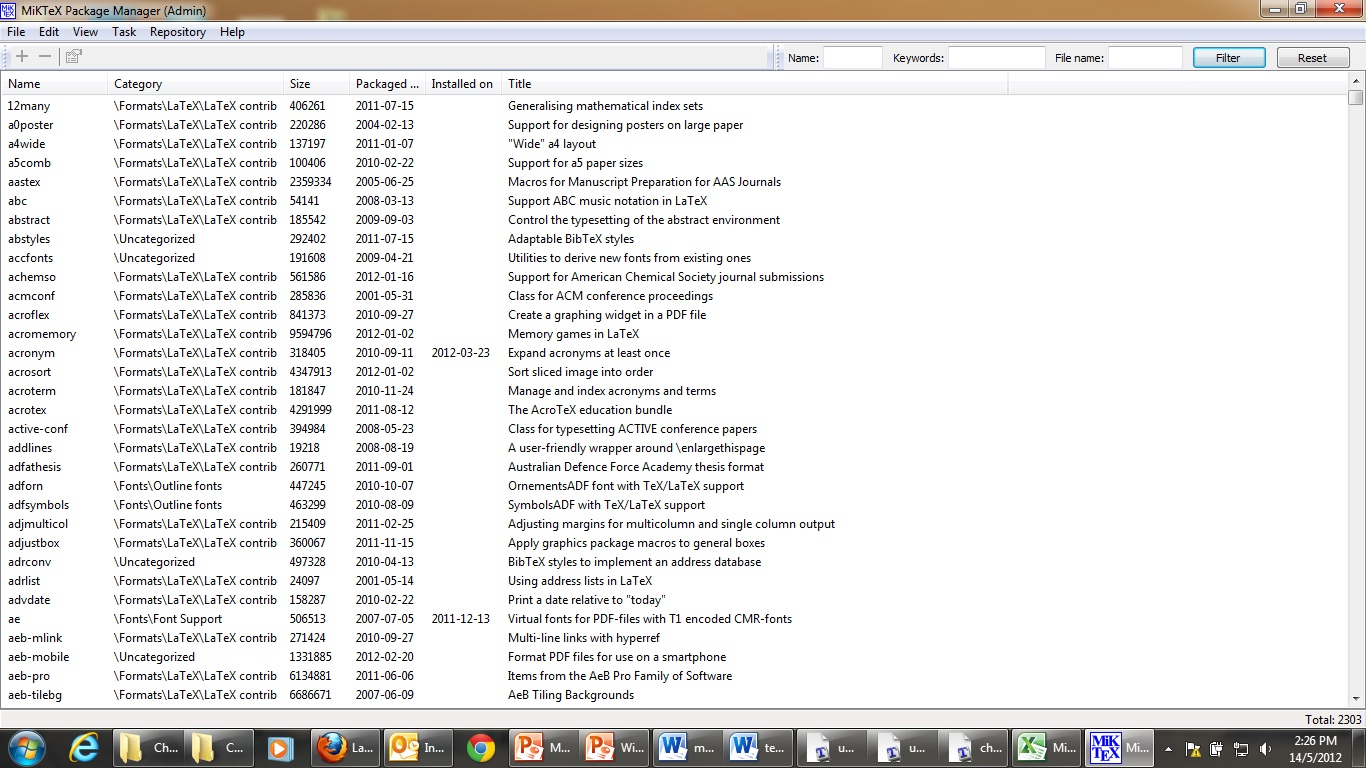
\includegraphics[width=1.00\textwidth]{admin_package} 
	\caption{Package Manager GUI}
	\label{fig2:package_manager}
\end{figure}

\section{Document file}

Using any text editor you can make a document file. Such raw text is referred to as {\LaTeX} source. Using the LaTeX program, it is converted to a beautifully formatted document. The content of the document is typed as plain text into one or more \verb+.tex+ files. Raw bibliographic databases are in plain text files named with the suffix \verb+.bib+ which we name it as \verb+rujukan_ump+.\\

In this work, the user only need to create different \verb+.tex+ file for each chapter and the file is located in a separate folder. For example, \verb+chap1.tex+ is located in the \verb+Chap1+ folder while \verb+chap2.tex+ is located in \verb+Chap2+ folder and so on. Note that in the preamble file, in the \verb+\mainmatter+ section only two chapters are included. If you have more just add \verb+\chapter{METHODOLOGY}
\label{ch:tocloft}

\section{Parametric Representation of curves and surfaces}


[1] Rogers. David F., An introduction to NURBS with historical perspective. 2001 by Academic Press.


The standard for describing and modeling curves and surfaces in computer aided design (CAD) and computer graphics is NURBS, or NonUniform Rational B-Splines. Essentially, NURBS describe parametric curves and surfaces. Curves and surfaces are mathematically represented either explicitly, implicitly or parametrically.

In practice, curves and surfaces are generally bounded. When either an explicit or implicit representation is used, imposing the boundaries is awkward. In contrast, the boundaries for a parametrically represented curve or surface are provided by the restective parameter ranges. In addition, the parameter range for a parametric curve also specifies a natural traversal direction along the curve. For example, specifying a curve requires one parameter while specifying a surface requires 2 parameters.

In general, a parametric curve representation of a 3D curve takes the mathematical functional form of x=f(t), y=g)t), and z=h(t), where t is the independent parameter. By extension, a parametric surface representation takes the form of x=f(u,w), y=g(u,w), z=h(u,w), where u and w are independent parameters. When compared to either explicit or implicit formulations, this parametric representation is extremely flexible. The representation is axis independent, easily represented by multiple-valued functions, can have infinite derivatives, and extended degrees of freedom.  To have more degrees of freedom additional independent parameters can be added.

\section{Continuity of curves and surfaces}

There are two kinds of continuity, or smoothness, associated with parametric curves and surfaces known as geometric continuity and parametric continuity. Simplistically, you can think of geometric continuity as physical and parametric continuity as mathematical. Geometric continuity is less restrictive than parametric continuity.




\section{Advantages of Parametric Representations in CNC}



\section{Parametric representation to CNC G-Codes}






All auto-numbered headings get entered in the Table of Contents (ToC) automatically. Entries for the ToC are recorded each time you process your document, and reproduced the next time you process it, so you need to re-run {\LaTeX} one extra time to ensure that all ToC page number references are correctly calculated. The commands \verb+\listoffigures+ and \verb+\listoftables+ work in exactly the same way as \verb+\tableofcontents+ to automatically list all your tables and figures. Note that, to have your figures or tables listed in list of figures or tables the command \verb+\ref{}+ must be used for referring the designated figure or table. Details on this will be given the following chapters.\\

The primary way to build a table is to use the tabular environment. Here's an example:

\begin{tabular}[t]{|l|ccccc|c|}
\multicolumn{7}{c}{USAMTS Scores Round 1}\\\hline
Name&\#1&\#2&\#3&\#4&\#5&Total\\\hline
John Doe&5&5&3&2&1&16\\
Jane Doe&5&5&5&4&5&24\\
Richard Feynman&5&5&5&5&5&25\\\hline
\end{tabular}

When you typeset that code, you should see a simple table like this one. Read through the following general description of the tabular environment to understand how the code above produced the table.\\

General form of the tabular environment:
\verb+\begin{tabular}[alignment]{columns}+
\verb+rows+
\verb+\end{tabular}+\\

\textbf{alignment} - put either b or t, or omit this completely. This determines how your table is vertically positioned with the text around it. This entry is not too important - experiment using different values (or omitting it) when you have a table in the midst of a document to get a better feel for it.\\

\textbf{columns} - this describes the number of columns and the alignment of each column. Put r for a right-justified column, c for a centered column, and l for a left-justified column. Put a | if you want a vertical line between columns. For example, the column declaration \verb+{||rr|cc|l}+ will produce a table that has 2 vertical lines on the left, then two columns that are right-justified, then a vertical line, then 2 columns that are centered, then another vertical line, then a left-justified column. There are more complicating things that you can do, and even more complicated things if you include the array packing in your document (check a good LaTeX book for more details), but for most tables, the options we've described here are sufficient.\\

\textbf{rows} - You can have as many rows as you like. For each row, you need an entry for each column. Each of these entries is separated by an \verb+&+. Use \verb+\\+ to indicate that your input for that row is finished. Hence, if your column declaration was \verb+{cccc}+, a possible row entry could be \verb+5&5&5&5\\+
\\

If you wish for one row to have fewer columns (i.e. one column takes up several of the usual table columns), use the command \verb+\multicolumn+. In the example above, we had as our first row\\

\verb+\multicolumn{7}{c}{USAMTS Scores Round 1}\\+

The first \verb+{ }+ indicates how many regular columns this entry will take up. The second \verb+{ }+ indicates whether the text in this entry is right (r), left (l) or center (c) justified. The final \verb+{ }+ contains our entry. As with the regular column declaration, use | if you want a vertical line before or after the entry of \verb+\multicolumn+.\\

In general, you can use \verb+\vline+ to introduce a vertical line anywhere in a table (try putting one between John and Nash in the example below and see what happens).\\

Finally, at the end of some of the rows in our example, we have the command \verb+\hline+. This produces a horizontal line after the row it follows. If you want a horizontal line atop a table, use \verb+\hline+ right before the first row. If you only want a horizontal line under a portion of the row, use \verb+\cline{start column-end column}+ as indicated in the example below:\\

\begin{tabular}[t]{|l|l|cccc|c|}\hline
\multicolumn{7}{|c|}{USAMTS Final Scores by Round}\\\hline
Medal&Name&\#1&\#2&\#3&\#4&Total\\\hline\hline
&Richard Feynman&25&25&25&25&100\\\cline{3-7}
Gold&Albert Einstein&25&25&25&25&100\\\cline{3-7}
&Marie Curie&25&24&24&25&98\\\hline
Silver&John Nash&20&20&25&24&89\\\hline
&Jane Doe&23&\multicolumn{2}{c}{None}&25&48\\\cline{3-7}
None&John Doe&\multicolumn{2}{c}{None}&25&20&45\\\cline{3-7}
&Lazy Person&5&\multicolumn{3}{c|}{None}&5\\\hline
\end{tabular}

When you typeset this, you should get output like this. Note how we made a double horizontal line after the table headings.\\

Finally, sometimes you'll want to create a table that consists solely of items in math mode. For such a table, use the array environment. The array environment works exactly like tabular, except that all its entries are rendered in math mode:

\[\begin{array}[b]{ccc}
x&y&z\\
y&x&z\\
1&2&3
\end{array}\]

Change both array declarations to tabular and delete the \verb+\[+ and \verb+\]+ and see what happens. You can do a number of other things with the array and tabular environments, but the above should cover most of what you'll want to do with them.\\

If you build a table in which some entries are text that will take up multiple lines, you'll probably want to learn about boxes (below).

+ to the list. Make sure you have created the designated folder and file for that chapter. \\

To keep thing simple so that user can directly use the application, open the \verb+chap1.tex+ in \verb+Chap1+ folder. Initially you will have a blank document. This document will contain all your writing for a chapter. For subsequent chapter create another document file. An example of completed document file is shown in Figure \ref{fig1:example_file}.

\begin{figure}
	\centering
	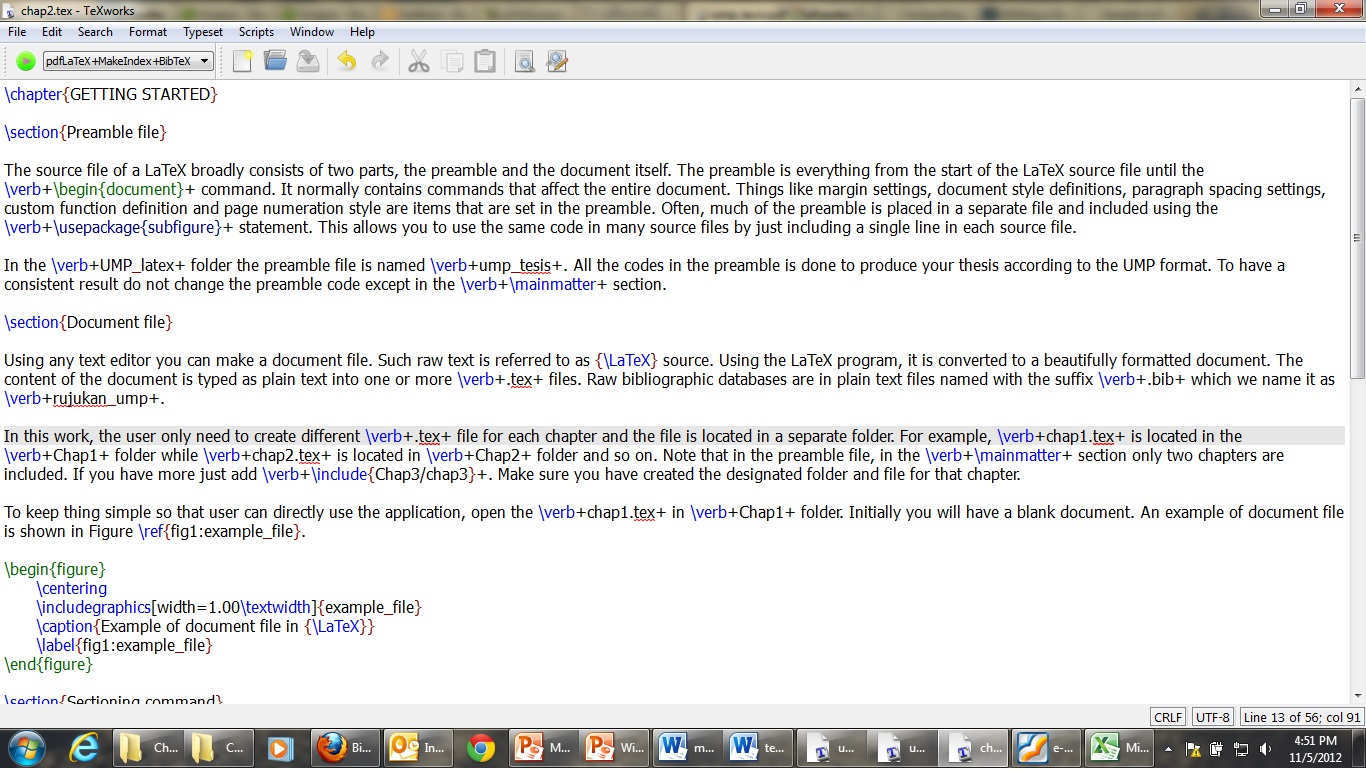
\includegraphics[width=1.00\textwidth]{example_file} 
	\caption{Example of document file in {\LaTeX}}
	\label{fig1:example_file}
\end{figure}

\section{Typesetting your file and viewing output pdf file}
Once you are ready to take a look at how your document will appear you typeset it with the default engine, pdflatex out of the box, by simply using the \verb+Typeset+ command.\\

Assuming the document was successfully typeset the pdf file will automatically open in a separate preview window.








\chapter{LITERATURE SURVEY}

\section{Introduction}

By default {\LaTeX} has its own standard format. This include paragraph alignment, paragraph indents, line spacing, abstracts, references and appendixes.  To comply with UMP thesis standards we have developed a custom coding to the preamble file that enable {\LaTeX} to produce  document according to the UMP standard formatting. This will make sure a uniform and error free format of your thesis. This chapter will cover techniques to format material in the document you create.

\section{Sectioning command}

For producing large documents such as thesis it is more easier to split the content into parts using {\LaTeX} sectioning commands. {\LaTeX} provides 7 levels of depth for defining sections as in Table \ref{tab1:section_depth}. For getting started, start each document with \verb+\chapter{title}+. This will make sure your thesis is well organized. Notice that you do not need to specify section numbers; LaTeX will sort that out for you. In addition, all the titles of the sections are added automatically to the table of contents. Moreover, the link to each chapter, section, tables, figures etc. are also provided automatically by {\LaTeX}.

% Table generated by Excel2LaTeX from sheet 'Sheet1'

\begin{table}[htbp]
\caption{Comparison of \LaTeX-based or \LaTeX-supporting Equation Editors} 
\centering
\begin{tabularx}{1\linewidth}{lll}    \addlinespace
    \toprule
    Command & Level & Comment \\
    \toprule
    \verb+\part{part}+ & -1    & not in letters \\
    \verb+\chapter{section}+ & 0     & only books and reports \\
    \verb+\section{section}+ & 1     & not in letters \\
    \verb+\subsection{subsection}+ & 2     & not in letters \\
    \verb+\subsubsection{subsubsection}+ & 3     & not in letters \\
    \verb+\paragraph{paragraph}+ & 4     & not in letters \\
    \verb+\subparagraph{subparagraph}+ & 5     & not in letters \\
    \bottomrule
    \end{tabularx}%
  \label{tab1:section_depth}%
\end{table}%

\section{Font Sizes and Styles}

To change the font size, use any one of the following commands. To change it for just a portion of the page, enclose that potion in \verb+{ }+ and have the relevant font size command occur right at the beginning of the text inside the curly braces. In order from smallest to largest, the font sizes you can use are:
\\
{\tiny{\verb+\tiny+}} \\
{\scriptsize{\verb+\scriptsize+}} \\
{\footnotesize{\verb+\footnotesize+}} \\
{\small{\verb+\small+}} \\
{\normalsize{\verb+\normalsize+}} \\
{\large{\verb+\large+}} \\
{\Large{\verb+\Large+}} \\
{\LARGE{\verb+\LARGE+}} \\
{\huge{\verb+\huge+}} \\ 
{\Huge{\verb+\Huge+}} \\

Try this out; the effects should be pretty clear:\\

When I was born, I was {\small small}. Actually, {\scriptsize I was very small}. When I got older, I thought some day {\Large I would be large}, {\Huge maybe even gigantic}. But instead, I'm not even normalsize. {\small I'm still small.}\\

Here is a simple example that will probably show you all you need to know about bold, italics, and underlining.\\

When something is \emph{really}, \textbf{really} important, you can \underline{underline it}, \emph{italicize it}, \textbf{bold it}. If you \underline{\textbf{\emph{must do all three}}}, then you can nest them.\\

Here is another example that demonstrates font families:\\

You may want to write things \textsf{in a sans-serif font}, or \texttt{in a typewriter font}, or \textsl{in a slanted font} (which is \emph{slightly different} than italics). Sometimes it pays \textsc{to write things in small capitals}. You can next go to \textbf{bold and then \textsl{bold and slanted} and then back to just bold} again.

\section{Spacing}

There are a few spacing items you'll find useful in {\LaTeX}. First, you can force a normal-size space (as between words) by using a single backslash followed by a space. This is particularly useful after periods: LaTeX interprets periods as ends of sentences, so it puts extra space after them, but if a period doesn't in fact end a sentence, you don't want that extra space. Try this to see an example.\\

When Mr. Rogers read this, he was confused because the first sentence was only two words long. Mrs.\ Rogers wasn't confused at all.\\

In math mode, it's a little different. LaTeX ignores normal spaces in math mode, so all three of the following will come out the same:\\

Spacing in math mode:

$x + y$

$x     +       y$

$x+y$
\\
Notice that the three math expressions come out all exactly the same. In general, you can trust math mode to space things out right rather than forcing any special spacing. This means that you should write formulas in your source document to be easily readable (by you), and trust LaTeX to do the right spacing.\\

However, if you do need to tweak the spacing in math mode, there are some special commands:
\, 	a small space
\: 	a medium space
\; 	a large space
\quad 	a really large space
\qquad 	a huge space
\! 	a negative space (moves things back to the left)\\

Here are examples of these in action:

$x+y$

$x+\,y$

$x+\:y$

$x+\;y$

$x+\quad y$

$x+\qquad y$

$x+\!y$

\subsection{Justification (Centering, etc)}

We can center text using
\\
\\
\verb+\begin{center}+\\
text\\
\verb+\end{center}+
\\
\\
and can justify it left or right with
\\
\\
\verb+\begin{flushleft}+\\
text\\
\verb+\end{flushleft}+\\
\\
\verb+\begin{flushright}+\\
text\\
\verb+\end{flushright}+\\
\\
\begin{center}
Fourscore and seven years ago our fathers brought forth on this continent a new nation, conceived in liberty and dedicated to the
proposition that all men are created equal.
\end{center}

\begin{flushleft}
Now we are engaged in a great civil war, testing whether that nation or any nation so conceived and so dedicated can long endure. We are met on a great battlefield of that war. We have come to dedicate a portion of it as a final resting place for those who died here that the nation might live. This we may, in all propriety do. But in a larger sense, we cannot dedicate, we cannot consecrate, we cannot hallow this ground. The brave men, living and dead who struggled here have hallowed it far above our poor power to add or detract. The world will little note nor long remember what we say here, but it can never forget what they did here.
\end{flushleft}

\begin{flushright}
It is rather for us the living, we here be dedicated to the great task remaining before us--that from these honored dead we take
increased devotion to that cause for which they here gave the last full measure of devotion--that we here highly resolve that these dead shall not have died in vain, that this nation shall have a new birth of freedom, and that government of the people, by the people, for the people shall not perish from the earth.
\end{flushright}


\chapter{METHODOLOGY}
\label{ch:tocloft}

\section{Parametric Representation of curves and surfaces}


[1] Rogers. David F., An introduction to NURBS with historical perspective. 2001 by Academic Press.


The standard for describing and modeling curves and surfaces in computer aided design (CAD) and computer graphics is NURBS, or NonUniform Rational B-Splines. Essentially, NURBS describe parametric curves and surfaces. Curves and surfaces are mathematically represented either explicitly, implicitly or parametrically.

In practice, curves and surfaces are generally bounded. When either an explicit or implicit representation is used, imposing the boundaries is awkward. In contrast, the boundaries for a parametrically represented curve or surface are provided by the restective parameter ranges. In addition, the parameter range for a parametric curve also specifies a natural traversal direction along the curve. For example, specifying a curve requires one parameter while specifying a surface requires 2 parameters.

In general, a parametric curve representation of a 3D curve takes the mathematical functional form of x=f(t), y=g)t), and z=h(t), where t is the independent parameter. By extension, a parametric surface representation takes the form of x=f(u,w), y=g(u,w), z=h(u,w), where u and w are independent parameters. When compared to either explicit or implicit formulations, this parametric representation is extremely flexible. The representation is axis independent, easily represented by multiple-valued functions, can have infinite derivatives, and extended degrees of freedom.  To have more degrees of freedom additional independent parameters can be added.

\section{Continuity of curves and surfaces}

There are two kinds of continuity, or smoothness, associated with parametric curves and surfaces known as geometric continuity and parametric continuity. Simplistically, you can think of geometric continuity as physical and parametric continuity as mathematical. Geometric continuity is less restrictive than parametric continuity.




\section{Advantages of Parametric Representations in CNC}



\section{Parametric representation to CNC G-Codes}






All auto-numbered headings get entered in the Table of Contents (ToC) automatically. Entries for the ToC are recorded each time you process your document, and reproduced the next time you process it, so you need to re-run {\LaTeX} one extra time to ensure that all ToC page number references are correctly calculated. The commands \verb+\listoffigures+ and \verb+\listoftables+ work in exactly the same way as \verb+\tableofcontents+ to automatically list all your tables and figures. Note that, to have your figures or tables listed in list of figures or tables the command \verb+\ref{}+ must be used for referring the designated figure or table. Details on this will be given the following chapters.\\

The primary way to build a table is to use the tabular environment. Here's an example:

\begin{tabular}[t]{|l|ccccc|c|}
\multicolumn{7}{c}{USAMTS Scores Round 1}\\\hline
Name&\#1&\#2&\#3&\#4&\#5&Total\\\hline
John Doe&5&5&3&2&1&16\\
Jane Doe&5&5&5&4&5&24\\
Richard Feynman&5&5&5&5&5&25\\\hline
\end{tabular}

When you typeset that code, you should see a simple table like this one. Read through the following general description of the tabular environment to understand how the code above produced the table.\\

General form of the tabular environment:
\verb+\begin{tabular}[alignment]{columns}+
\verb+rows+
\verb+\end{tabular}+\\

\textbf{alignment} - put either b or t, or omit this completely. This determines how your table is vertically positioned with the text around it. This entry is not too important - experiment using different values (or omitting it) when you have a table in the midst of a document to get a better feel for it.\\

\textbf{columns} - this describes the number of columns and the alignment of each column. Put r for a right-justified column, c for a centered column, and l for a left-justified column. Put a | if you want a vertical line between columns. For example, the column declaration \verb+{||rr|cc|l}+ will produce a table that has 2 vertical lines on the left, then two columns that are right-justified, then a vertical line, then 2 columns that are centered, then another vertical line, then a left-justified column. There are more complicating things that you can do, and even more complicated things if you include the array packing in your document (check a good LaTeX book for more details), but for most tables, the options we've described here are sufficient.\\

\textbf{rows} - You can have as many rows as you like. For each row, you need an entry for each column. Each of these entries is separated by an \verb+&+. Use \verb+\\+ to indicate that your input for that row is finished. Hence, if your column declaration was \verb+{cccc}+, a possible row entry could be \verb+5&5&5&5\\+
\\

If you wish for one row to have fewer columns (i.e. one column takes up several of the usual table columns), use the command \verb+\multicolumn+. In the example above, we had as our first row\\

\verb+\multicolumn{7}{c}{USAMTS Scores Round 1}\\+

The first \verb+{ }+ indicates how many regular columns this entry will take up. The second \verb+{ }+ indicates whether the text in this entry is right (r), left (l) or center (c) justified. The final \verb+{ }+ contains our entry. As with the regular column declaration, use | if you want a vertical line before or after the entry of \verb+\multicolumn+.\\

In general, you can use \verb+\vline+ to introduce a vertical line anywhere in a table (try putting one between John and Nash in the example below and see what happens).\\

Finally, at the end of some of the rows in our example, we have the command \verb+\hline+. This produces a horizontal line after the row it follows. If you want a horizontal line atop a table, use \verb+\hline+ right before the first row. If you only want a horizontal line under a portion of the row, use \verb+\cline{start column-end column}+ as indicated in the example below:\\

\begin{tabular}[t]{|l|l|cccc|c|}\hline
\multicolumn{7}{|c|}{USAMTS Final Scores by Round}\\\hline
Medal&Name&\#1&\#2&\#3&\#4&Total\\\hline\hline
&Richard Feynman&25&25&25&25&100\\\cline{3-7}
Gold&Albert Einstein&25&25&25&25&100\\\cline{3-7}
&Marie Curie&25&24&24&25&98\\\hline
Silver&John Nash&20&20&25&24&89\\\hline
&Jane Doe&23&\multicolumn{2}{c}{None}&25&48\\\cline{3-7}
None&John Doe&\multicolumn{2}{c}{None}&25&20&45\\\cline{3-7}
&Lazy Person&5&\multicolumn{3}{c|}{None}&5\\\hline
\end{tabular}

When you typeset this, you should get output like this. Note how we made a double horizontal line after the table headings.\\

Finally, sometimes you'll want to create a table that consists solely of items in math mode. For such a table, use the array environment. The array environment works exactly like tabular, except that all its entries are rendered in math mode:

\[\begin{array}[b]{ccc}
x&y&z\\
y&x&z\\
1&2&3
\end{array}\]

Change both array declarations to tabular and delete the \verb+\[+ and \verb+\]+ and see what happens. You can do a number of other things with the array and tabular environments, but the above should cover most of what you'll want to do with them.\\

If you build a table in which some entries are text that will take up multiple lines, you'll probably want to learn about boxes (below).


\chapter{RESULTS}

\section{Introduction}
References is automatically organize in your document. Any addition or modification to reference in the text will be automatically update the lists of references. There are two ways to insert your references into {\LaTeX}:

\begin{itemize}
\item you can embed them within the document itself. It's simpler, but it can be time-consuming if you are writing several papers about similar subjects so that you often have to cite the same books.
\item you can store them in an external BibTeX file and then link them via a command to your current document and use a Bibtex style to define how they appear. This way you can create a small database of the references you might use and simply link them, letting {\LaTeX} work for you.
\end{itemize}

We will focus on the second approach since it is more efficient to handle large database.\\

Although your preferred software manager can generate it automatically for you and you save it in \verb+whateverthename.bib+ file, I would advise you to manually check the details again.

\section{Citing references}
Type \verb+\cite{citationkey}+ where you want to cite a reference in your .tex document. If you don’t want an in text citation, but still want the reference to appear in the bibliography, use \verb+\nocite{citationkey}+.\\

To include a page number in your in-text citation put it in square brackets before the citation key: \verb+\cite[p. 215]{citationkey}+.\\

To cite multiple references include all the citation keys within the curly brackets separated by commas: \verb+\cite{citation01,citation02,citation03}+.\\

For UMP template, we will be using APA styles. \textbf{natbib} package in preamble file is used for author-date citations. Natbib uses the command \verb+\citep{...}+ for a citation in brackets, such as: (Koppe, 2010) or \citet{Carvalho-etal-2008} and \verb+\citet{...}+ for a citation where only the year is in brackets, such as: Koppe (2010). Here, the command \verb+\cite+ will produce the same output as \verb+\citep+ or \citep{Carvalho-etal-2009}



\chapter{CONCLUSION}

\section{Introduction}
This template is to guide user on current UMP Thesis template using {\LaTeX}. Learning {\LaTeX} might be an arduous task at first, especially when it gives continuous error message (hey! those error message helps). The error message can be tricky at times and sometimes, it gives you an important warning as simple as missing \{, but you need to look carefully on what they mean and how to solve them.\\

Forget about error messages, simply learn it using this guide, you will get used to {\LaTeX} in really short time.

\section{Chapter and Section}
Don't worry about the numbering chapter, section and subsection, using \verb+\chapter+, \verb+\section+ and \verb+\subsection+ command, {\LaTeX} will give automatic output for you, as long as you insert the correct input and command at the correct place. For chapters, call your \verb+\chapter+ in the preamble file under \verb+\mainmatter+ according to the arrangement of your thesis.

\subsection{Subsection}
Some text here.\\

If you want to start new paragraph, put \verb+\\+ at the end of your paragraph before this paragraph. Nothing much here, keep reading this long text, I just wanted to make this paraghraph longer. Try removing \verb+\\+ from previous paragraph and see what happened.\\

\noindent Insert \verb+\noindent+ at the beginning of the sentence in this paragraph if you want new paragraph but with no indentation.

\section{UMP Table Format}
We will start with table formatting. In chapter \ref{ch:tocloft}, you have learnt to use tabular environment. In this section, following UMP format, we will be using tabularx environment instead. \verb+tabularx+ environment gives full line table compared to \verb+tabular+ environment, which gives table's line according to its size.\\

\noindent You could see the difference here,

\begin{table}[h!]
\caption{Using tabularx environment} 
\begin{tabularx}{1\linewidth}{XXX}    \addlinespace
    \toprule
    Name & Score & Ranking \\
    \toprule
    Ali & 59 & 2 \\
    Shah & 77 & 1 \\
    \bottomrule
    \end{tabularx}
\end{table}

\begin{table}[h!]
\caption{Using tabular environment}
\begin{tabular}{lll}
\toprule
    Name & Score & Ranking \\
    \toprule
    Ali & 59 & 2 \\
    Shah & 77 & 1 \\
    \bottomrule
\end{tabular}
\end{table}

\cleardoublepage %use this code when you want to finish the part at this page and continue the next part in the next page
 
You might encounter this problem when you have a really really long text. 

\begin{table}[h!]
\caption{What is wrong with my table?} 
\begin{tabularx}{1\linewidth}{XXX}    \addlinespace
    \toprule
    Name & Score & Ranking \\
    \toprule
    really really really really really really really long names & 59 & 2 \\
    Shah & 77 & 1 \\
    \bottomrule
    \end{tabularx}
\end{table}

Say, you have a really long text in the line, you could change the size of each column by changing \verb+{XXX}+ to \verb+{p{desired width}p{desired width}p{desired width}}+

\begin{table}[h!]
\caption{Change column width}
\begin{tabularx}{1\linewidth}{p{10.0cm}XX}    \addlinespace
    \toprule
    Name & Gender & Ranking \\
    \toprule
    really really really really really really really long names & 59 & 2 \\
    Shah & 77 & 1 \\
    \bottomrule
    \end{tabularx}
\end{table}

Now, try making the table header text in bold.

\section{Large landscape table}
Yes, we could hear you! You probably need this large rotating table when dealing with quite numbers of columns.\\

First, enable \verb+usepackage{rotating}+ which I have done it for you in preamble file. If you don't need the rotating table, don't think twice, you can simply delete this package.\\

\begin{sidewaystable}[h!]
    \centering
\caption{Wide table}
\begin{tabularx}{\textwidth}{XXXX}
    \toprule
what are we trying to do here & something  & some text & something something  \\
    \toprule
11111111111111111 & 22222222222  & 3333333333 & 4444444444  \\
555555555 & 6666666666  & 777777777 & 88888888  \\
\bottomrule
\end{tabularx}
\begin{flushleft}
\textsuperscript{a} Things \\
\textsuperscript{b} Things \\
\textsuperscript{c} Things \\
\end{flushleft}
\end{sidewaystable}

Before that, do you realise you don't have to worry about the table's caption numbering? This works for figures too. You will see this later.

\cleardoublepage

 \section{Figure, Label and Cross-references}
 You probably expect the instructions on how to insert figure but no, the instructions are there before. See
 \verb+chap1.tex+ where I inserted Package Manager GUI (Figure \ref{fig2:package_manager}).\\
 
 Also, see how \verb+\ref+ and \verb+\label+ command to make hyper-reference for table, equations or sections.. Then, try to use them with equations, tables and sections.

\section{Itemize and lists}
{\LaTeX} supports two types of lists: \textbf{enumerate} produces numbered lists, while \textbf{itemize} is for bulleted lists. Each item is defined by \verb+\item+. For example, the following code\\

\verb+\begin{enumerate}+\\
\indent\verb+\item First thing+\\
 \indent\verb+\item Second thing+\\
 \indent\verb+\begin{itemize}+\\
 \indent\verb+\item A sub-thing+\\
 \indent\verb+\item Another sub-thing+\\
 \indent\verb+\end{itemize}+\\
\indent\verb+\item Third thing+\\
\indent\verb+\end{enumerate}+\\
 
 \noindent will produce things like this\\
 \begin{enumerate}
     \item First thing
     \item Second thing
     \begin{itemize}
     \item A sub-thing
     \item Another sub-thing
     \end{itemize}
     \item Third thing
     \end{enumerate}

\section{Equations}
One of the main reasons for writing documents in {\LaTeX} is because it is really good at typesetting equations. Equations are written in ‘math mode’.

\subsection{Inserting equations}
You can enter math mode with an opening and closing dollar sign \$. This can be used to write mathematical symbols within a sentence. For example, typing \$1+2=3\$ produces $1 + 2 = 3$.\\

If you want a “displayed” equation on its own line use \$\$...\$\$. For example, \$\$1+2=3\$\$ produces $$1+2=3$$.

\noindent or this code \verb+\[...\]+, also produces the same output.

\[ 1+2=3 \]

For a numbered displayed equation, use \verb+\begin{equation}...\end{equation}+.
For example, \verb+\begin{equation}1+\verb+2=3\end{equation}+ produces: 
\begin{equation}
\label{equation}
1+2=3
\end{equation}
The equation number \ref{equation} refers to the chapter number, this will only appear if you are using a document class with chapters, such as report.\\

Refer \url{https://www.overleaf.com/learn/latex/Mathematical_expressions} for more symbols and instructions for equations.



 \section{Flowchart}
 
Students definitely need flowchart to present the process of your research. Here, I am guiding you how to draw your flowchart. First, enable \verb+\usepackage[tikzpicture]+ and \verb+\usepackage[shapes,arrows]+, which in this template, I have done it for you.\\

Here are some basic shapes and arrows you will need in your flowchart. You could change the thickness, width or height of the shapes accordingly at \verb+%Define block styles+ in your \verb+tex file.+\\

Under \verb+%Place nodes+ commands, you can instruct {\LaTeX} where to place your shapes and its respective text. \verb+%Draw edges+ is used for drawing arrows in and out of your shapes.\\

Here, I will take one example\\

\verb+\node[block, below of=start](dc){Data collection}+. From this command, the instructions are \verb+["what shape", "location of the shape"]("whatever name"){"text"}+.\\

Figure \ref{fig:flowchartex} is the example of one full flowchart:\\

% Define block styles
\tikzstyle{decision} = [diamond, draw, thick, 
    text width=6.5em, text badly centered, inner sep=0pt]
\tikzstyle{block} = [rectangle, draw, thick, minimum width=6em, text centered, minimum height=3em, node distance=1.8cm]
\tikzstyle{line} = [draw, -latex']
\tikzstyle{cloud} = [draw, ellipse, thick, node distance=1.8cm,
    minimum height=3em]

\begin{figure}[h!]
\begin{center}
\vspace{5mm}
\begin{tikzpicture}[node distance = 3.5cm, auto]
    % Place nodes
    \node [cloud] (start) {Start};
    \node [block, below of=start] (dc) {Data collection};
    \node [block, below of=dc] (da) {Data analysis};
    \node [block, below of=da] (B) {Model B};
    \node [block, below of=B] (ce) {Computational experiment};
    \node [block, left of= B, node distance=3.8cm] (A) {Model A};
    \node [block, right of=B, node distance=5cm] (C) {Model C};

    \node [decision, below of=ce,node distance=3cm] (decide) {Is the data satisfied?};
    
    \node [block, below of=decide,node distance=3cm] (cs) {Comparative study};
    \node [block, below of=cs] (srp) {Solving real problem};
    \node [block, below of=srp] (dnc) {Discussion and conclusion};
    \node [cloud, below of=dnc ] (stop) {Stop};
    % Draw edges
    \path [line] (start) -- (dc);
    \path [line] (dc) -- (da);
    \path [line] (da) -- (B);
    \path [line] (da) -- (A);
    \path [line] (da) -- (C);
    \path [line] (B) -- (ce);
    \path [line] (A) |- (ce);
    \path [line] (C) |- (ce);
    \path [line] (ce) -- (decide);
    \path [line] (decide) -- node [, color=black] {Yes} (cs);
    \path [line] (decide) -- (cs);
    \path [line] (cs) -- (srp);
    \path [line] (srp) -- (dnc);
    \path [line] (dnc) -- (stop);
    \path [line] (decide.east) --+ (7cm,0) |- (da) node [near start,right] {No};
\end{tikzpicture}
\caption{Flow chart of operational framework}
	\label{fig:flowchartex}
\end{center}
\end{figure}
\cleardoublepage



\renewcommand\bibname{REFERENCES}
\bibliographystyle{apacite}
\renewcommand{\doiprefix}{}
\renewcommand{\doi}[1]{https://doi.org/#1}
\titlespacing*{\chapter}{0pt}{-60pt}{40pt}
% this command makes single spacing for reference
\begingroup
    \setlength{\bibsep}{10pt}
    \setstretch{1}
    \bibliography{rujukan}
\endgroup
%\bibliography{rujukan}  
\titlespacing*{\chapter}{0pt}{50pt}{40pt}
\cleardoublepage

% Put your appendices here. Make sure you create a specific folder for each appendix.

\appendix
\let\appendixpagenameorig\appendixpagename
\renewcommand{\appendixpagename}{\normalfont\MakeUppercase\appendixpagenameorig}
\renewcommand{\appendixtocname}{APPENDICES}
\expandafter\def\expandafter\appendixpagename%
\expandafter{\expandafter\Large\appendixpagename}
\appendixpage
\cleardoublepage
\titlespacing*{\chapter}{0pt}{-60pt}{40pt}




%% \section{APPENDIX CHAPTER 1}\label{APPENDIX CHAPTER 1}

%% \noindent
%% NO CONTENTS.\\



%% \clearpage
%% \pagebreak



%% \section{APPENDIX CHAPTER 2}\label{APPENDIX CHAPTER 2}

%% \noindent
%% NO CONTENTS.\\


%% \clearpage
%% \pagebreak

\section{APPENDIX CHAPTER 3}\label{APPENDIX CHAPTER 3}

\subsection{About Side Effects in Computations}
\label{app-Chap3-About Side Effects in Computations}


In computer science, an operation, function or expression is said to have a side effect if it modifies some state variable value(s) outside its local environment, which is to say if it has any observable effect other than its primary effect of returning a value to the invoker of the operation. Source: [\href{https://en.wikipedia.org/wiki/Side_effect_(computer_science)}{Side effect in computer science}].\\

It is extremely important that computing operations do not cause side effects unintentionally. The programmer must be aware of side effects if imperative programming paradigm is implemented, where the application state flows from one function to the next. The unintended changes in state information are basically side effects. If the change is intended (deliberate) then it is not a side effect. \\

For example, a global variable "count\_total\_lines" is intended to be incremented every time a specific local function executes, then it is not a side effect. When a second local function executes, it is also intended that the global variable "count\_total\_lines" be incremented. This is not a problem. \\

The side effect problems may exist if the program implements many global variables that are inter-related to each other in computations. Since there are many variables involved, it will be difficult to track which variable values should change, and which should not change. This is where side effects may occur. For example, if by mistake successive executions of different functions do not happen in the order as designed, then side effects will definitely occur. One example in computer science that creates side effect is a race condition. It was said that side effects are not only limited to state manipulation, in fact, interacting with the I/O, database, log system, APIs and anything else that can be controlled, has a side effect. \\

It is known that the functional programming paradigm aims to minimize or eliminate side effects. The lack of side effects in functional programming makes it easier to do formal verification of a program. Formal verification means verifying that the function executes correctly, and the execution also produces the correct results. \\

In general programming, there are many ways to reduce and minimize the occurrence of side effects. Proper naming of variables that separates global from local variables is helpful. Having the program flow design to be fully structured definitely helps. Program flows that are unstructured or haphazard invites disaster, especially the occurrence of side effects. \\

In practice, most applications will combined the declarative and imperative programming paradigms. There is a fine balancing act between the declarative (what do to) and imperative (how to do) paradigms, with more a shift in the community towards declarative programming. \\

This appendix is not meant to provide an exhaustive analysis on side-effects, a good read on it is provided at the URL link [\href{https://thejs.dev/jmitchell/what-are-side-effects-and-what-you-can-do-about-them-jws}{What are side effects and what you can do about them (2020).}]. 




%% ==============================
\clearpage
\pagebreak

\subsection{Realtime Computing Environment}
\label{app-chap3-Realtinme Computing Environment}


The official title of this thesis is "\textit{Realtime interpolation of parametric curves with chord-error and feedrate constraints.}" The word "realtime" is the first word in the title and it deserves to be discussed.\\

To a lay person, realtime means happening now, happening currently or immediately, or as it is happening, or occurring at the current instance or not happening in past time, or not occurring in delayed time. These interpretations are all correct. However, the interpretation of realtime in computing is different. This work satisfies both the layman and technical computing interpretations of realtime. \\

In layman's interpretation for the algorithm in this work, realtime means that as soon as the computation of the next interpolated point is completed, the interpolation algorithm will immediately send signals to the CNC machine to make that specific move. The cycle repeats for the next interpolated point until it reaches the end of the curve. This is the realtime according to the layman's interpretation. \\

Technically, in computing, real time is a guaranteed level of computer responsiveness within a specified time constraint, usually milliseconds or microseconds, between an event and its response deadline. This time delay between an event and its response is termed as time latency or just latency. \\

Real-time or real time describes various operations in computing or other processes that must guarantee response times within a specified time (deadline), usually a relatively short time. A real-time process is generally one that happens in defined time steps of maximum duration and fast enough to affect the environment in which it occurs, such as inputs to a computing system. Realtime does not mean fast or happening now. Realtime means it must be done before its deadline.\\

\clearpage
\pagebreak

The generally accepted technical definition of realtime is provided at URL [\href{https://en.wikipedia.org/wiki/Real-time_computing}{Real-time Computing}]. Real-time computing (RTC) is the computer science term for hardware and software systems subject to a "real-time constraint", for example from event to system response. Real-time programs must guarantee response within specified time constraints, often referred to as "deadlines"  or "maximum latency". \\

The interpolation algorithm developed in this work runs on a Real-Time Operating System (RTOS) and so makes the word "realtime" in its title accurate. The realtime requirements for timing latency of the algorithm's execution must be satisfied. \\

The LinuxCNC-Axis software that drives the G-Code signals generated by the algorithm runs on a realtime operating system (RTOS). If it is a non-RTOS, LinuxCNC-Axis software can only simulate running G-codes but not actually driving the electrical signals to the CNC machine. This is the first part of realtime in this thesis. \\

The next question is about the timing latency of computers in this work that will drive the G-Code signals. The maximum latency or deadline in this work is the time between the event of sending the signal to the time the CNC motors respond with the appropriate move. The signal travel time along the electrical wires is not a problem, since it is about 80 percent of the speed of light (almost instantaneous). The realtime requirement here is about the timing capability of the computer in sending repeated signals (worst case duration between a signal and its next signal). Sending a signal is an event, so the time between successive signals is a measure of latency. This worst case latency must be guaranteed for the computer.\\ 

Are the computers in this work capable of guaranteeing worst case latencies or deadlines to be considered realtime? The answer is definitely yes. It is confirmed by actual measurements, in which the results and discussions are provided in this document in section Cyclictest for Computer Latency Measurements [\ref{app4-Cyclictest for computer latency measurements}].  

 
%% ==================================================
\clearpage
\pagebreak

\subsection{Cyclictest for computer latency measurements}
\label{app4-Cyclictest for computer latency measurements}

In computing community, the cyclictest application program is a standardized shared code test that is used universally to measure computer hardware latencies. The results are captured in a tabular data format and plotted on a histogram. Essentially, the cyclictest code measures latency of the combined effect of the hardware, the firmware, and the operating system. \\

Cyclictest accurately and repeatedly measures the difference between a thread's intended wake-up time and the time at which it actually wakes up in order to provide statistics about the system's latencies. Cyclictest is most commonly used for benchmarking realtime (RT) systems. It is one of the most frequently used tools for evaluating the relative performance of real-time systems. Source: [\href{https://wiki.linuxfoundation.org/realtime/documentation/howto/tools/cyclictest/start}{Linux Foundation Cyclictest}] \\ 

\noindent
The results of cyclictest measurements in microseconds (us) for 10 million cycles (30 minutes run) in this work are as follows: 

\begin{enumerate}
	\item PASSED as RTOS. Histogram [\ref{Histogram-Latency-HP-Laptop-01-Debian10-10million-cycles.pdf}] shows a maximum latency value 42 (us) for HP-Laptop-01, on OS Debian 10 Kernel: 4.19.0-25-rt-amd64. 
	
	\item FAILED as RTOS. Histogram [\ref{Histogram-Latency-HP-Laptop-01-Ubuntu20-10million-cycles.pdf}] shows a maximum latency value 431 (us) for HP-Laptop-01, on OS Ubuntu 20.04 LTS Kernel: 5.15.0-86-lowlatency. 

	\item PASSED as RTOS. Histogram [\ref{Histogram-Latency-HP-Laptop-02-Debian10-10million-cycles.pdf}] shows a maximum latency value 46 (us) for HP-Laptop-02, on OS Debian 10 Kernel: 4.19.0-25-rt-amd64. 

    \item FAILED as RTOS. Histogram [\ref{Histogram-Latency-HP-Laptop-02-Ubuntu20-10million-cycles.pdf}] shows a maximum latency value 872 (us) for HP-Laptop-02, on OS Ubuntu 20.04 LTS Kernel: 5.15.0-86-lowlatency. 
\end{enumerate}

In the four(4) CPU Latency Performance Summary data tables at 
[\ref{tab-Debian10 HP-Laptop-01 CPU Performance}], 
[\ref{tab-Ubuntu20 HP-Laptop-01 CPU Performance}], 
[\ref{tab-Debian10 HP-Laptop-02 CPU Performance}], and
[\ref{tab-Ubuntu20 HP-Laptop-02 CPU Performance}], we can see that the average latencies for each of the 8-CPU cores as 2 (us) for RTOS and 8 (us) for non-RTOS. It is not the average latency that determines the RTOS status but the value of the worst case or maximum latency. The lower value for latency the  better.

%% ==================================================
\clearpage
\pagebreak

%% \begin{landscape}
\begin{figure}
\caption{Histogram-Latency-HP-Laptop-01-Debian10-10million-cycles}
\label{Histogram-Latency-HP-Laptop-01-Debian10-10million-cycles.pdf}
\centering
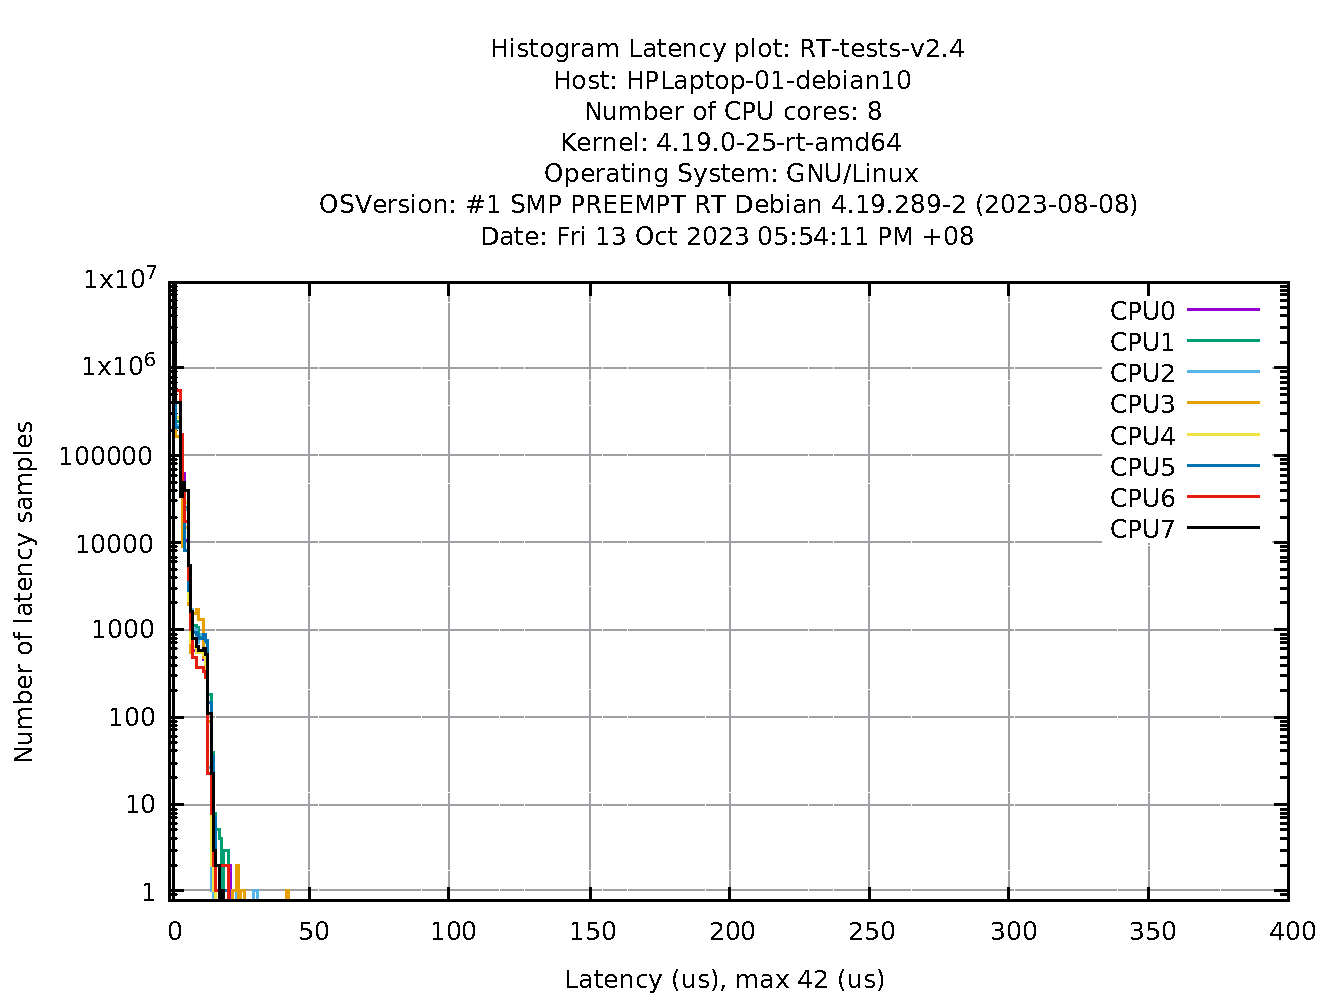
\includegraphics[width=1.00\textwidth]{Chap3/app-realtime/Histogram-Latency-HP-Laptop-01-Debian10-10million-cycles.pdf} 
\end{figure}	
%% \end{landscape}

\begin{figure}
\caption{Histogram-Latency-HP-Laptop-01-Ubuntu20-10million-cycles}
\label{Histogram-Latency-HP-Laptop-01-Ubuntu20-10million-cycles.pdf}
\centering
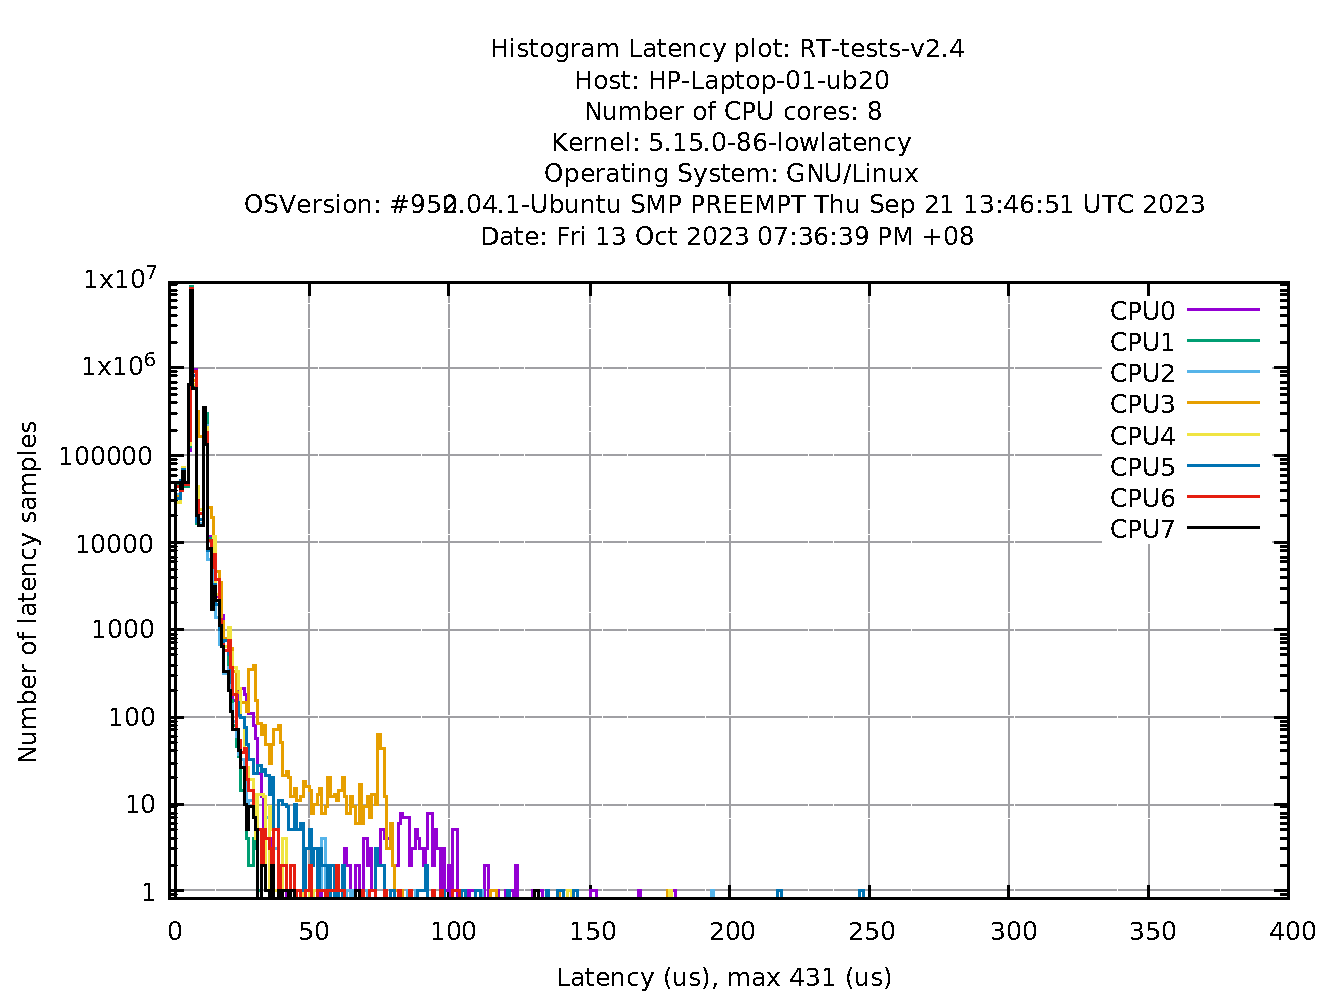
\includegraphics[width=1.00\textwidth]{Chap3/app-realtime/Histogram-Latency-HP-Laptop-01-Ubuntu20-10million-cycles.pdf} 
\end{figure}	

%% ==================================================
\clearpage
\pagebreak

\begin{figure}
\caption{Histogram-Latency-HP-Laptop-02-Debian10-10million-cycles}
\label  {Histogram-Latency-HP-Laptop-02-Debian10-10million-cycles.pdf}
\centering
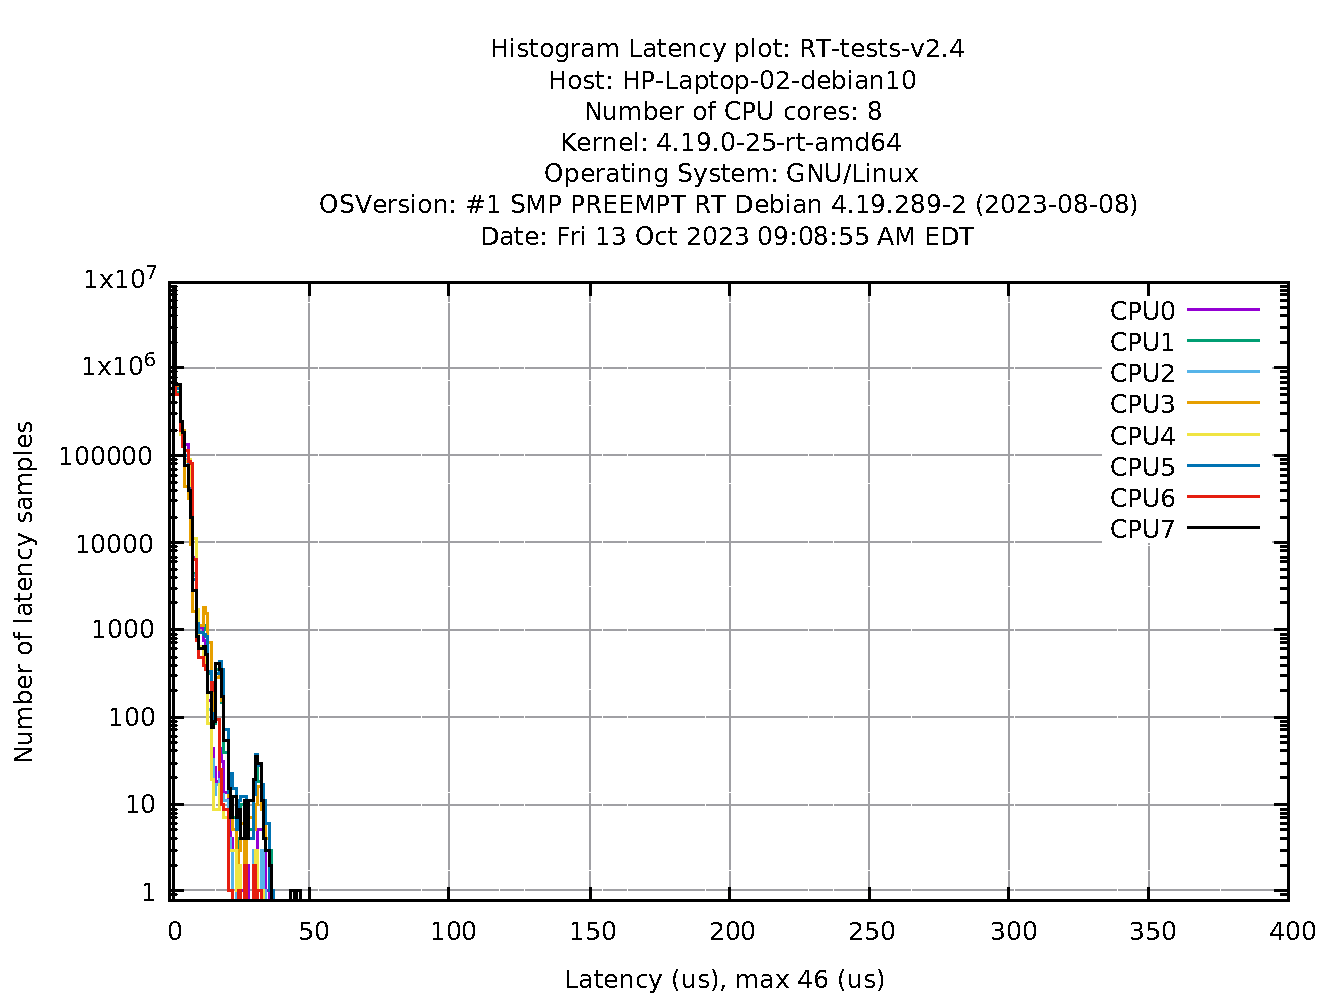
\includegraphics[width=1.00\textwidth]{Chap3/app-realtime/Histogram-Latency-HP-Laptop-02-Debian10-10million-cycles.pdf} 
\end{figure}	

\begin{figure}
\caption{Histogram-Latency-HP-Laptop-02-Ubuntu20-10million-cycles}
\label  {Histogram-Latency-HP-Laptop-02-Ubuntu20-10million-cycles.pdf}
\centering
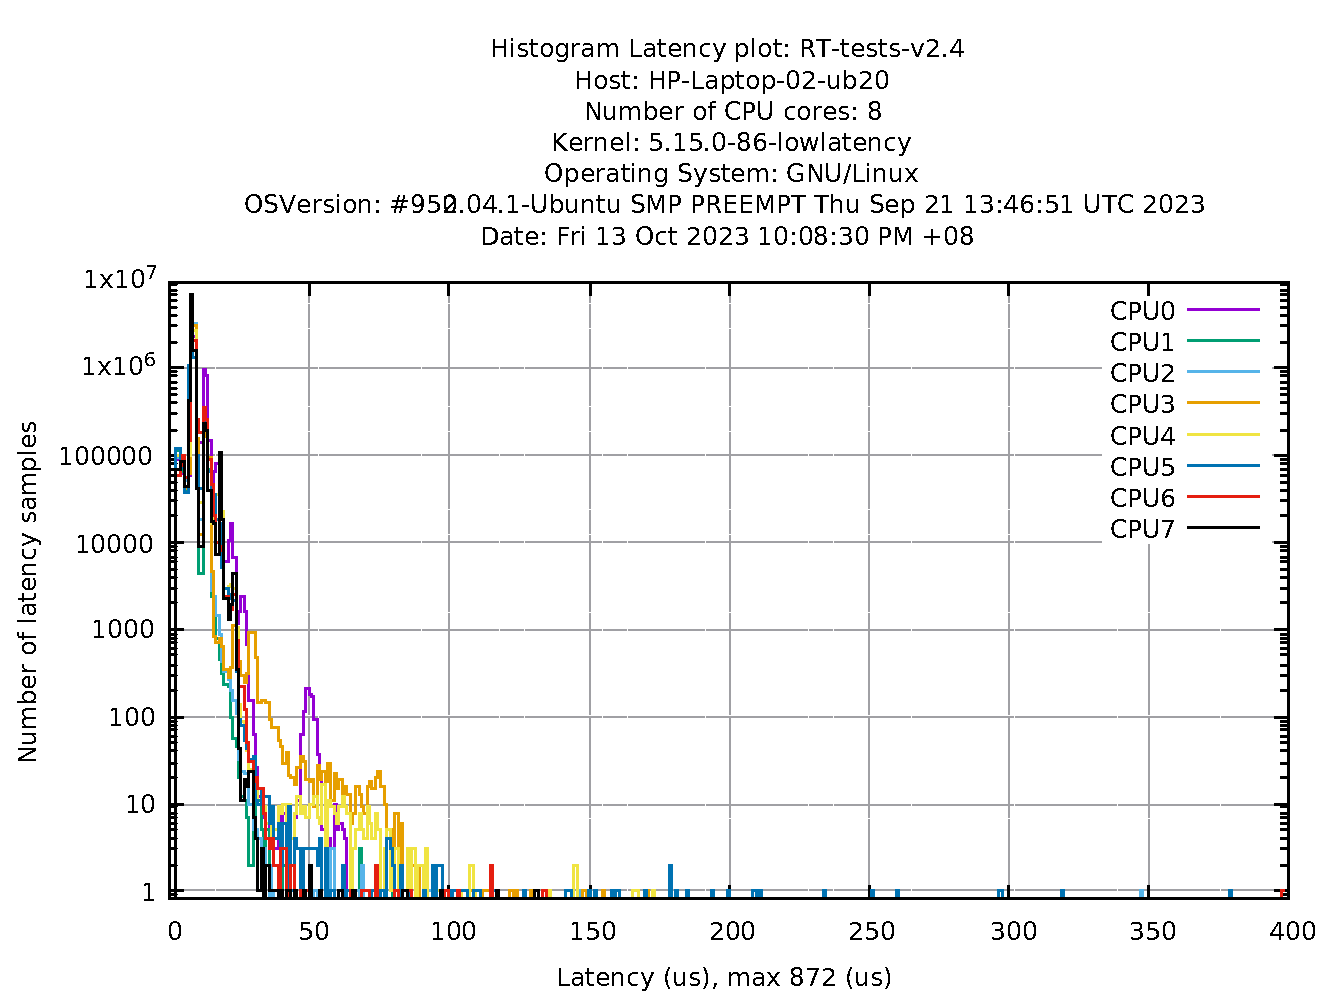
\includegraphics[width=1.00\textwidth]{Chap3/app-realtime/Histogram-Latency-HP-Laptop-02-Ubuntu20-10million-cycles.pdf} 
\end{figure}	


%% ==================================================
\clearpage
\pagebreak

\subsection{CPU Latency Performance Summary}

%% HP-LAPTOP-01-DEBIAN10 
\lstset{backgroundcolor=\color{white}, basicstyle=\linespread{0.92}\footnotesize, frame={topline, bottomline, leftline, rightline}}	
\begin{lstlisting}[caption={Debian10 HP-Laptop-01 CPU Performance}, label=tab-Debian10 HP-Laptop-01 CPU Performance]	
# Run for 10,000,000 cycles (approx 30 minutes)
# LATENCY (us)         CPU0  CPU1  CPU2  CPU3  CPU4  CPU5  CPU6  CPU7
# Min Latencies:       00002 00002 00002 00002 00002 00002 00002 00002
# Avg Latencies:       00002 00002 00002 00002 00002 00002 00002 00002
# Max Latencies:       00021 00020 00031 00042 00016 00020 00020 00019
# Histogram Overflows: 00000 00000 00000 00000 00000 00000 00000 00000
\end{lstlisting}

%% HP-LAPTOP-01-UBUNTU20 
\lstset{backgroundcolor=\color{white}, basicstyle=\linespread{0.92}\footnotesize, frame={topline, bottomline, leftline, rightline}}	
\begin{lstlisting}[caption={Ubuntu20 HP-Laptop-01 CPU Performance}, label=tab-Ubuntu20 HP-Laptop-01 CPU Performance]	
# Run for 10,000,000 cycles (approx 30 minutes)
# LATENCY (us)         CPU0  CPU1  CPU2  CPU3  CPU4  CPU5  CPU6  CPU7
# Min Latencies:       00003 00003 00003 00003 00003 00003 00003 00003
# Avg Latencies:       00008 00008 00008 00008 00008 00008 00008 00008
# Max Latencies:       00431 00040 00194 00178 00179 00247 00103 00131
# Histogram Overflows: 00001 00000 00000 00000 00000 00000 00000 00000
\end{lstlisting}

%% HP-LAPTOP-02-DEBIAN10 
\lstset{backgroundcolor=\color{white}, basicstyle=\linespread{0.92}\footnotesize, frame={topline, bottomline, leftline, rightline}}	
\begin{lstlisting}[caption={Debian10 HP-Laptop-02 CPU Performance}, label=tab-Debian10 HP-Laptop-02 CPU Performance]	
# Run for 10,000,000 cycles (approx 30 minutes)
# LATENCY (us)         CPU0  CPU1  CPU2  CPU3  CPU4  CPU5  CPU6  CPU7
# Min Latencies:       00002 00002 00002 00002 00002 00002 00002 00002
# Avg Latencies:       00002 00002 00002 00002 00002 00002 00002 00002
# Max Latencies:       00035 00037 00034 00036 00033 00037 00032 00046
# Histogram Overflows: 00000 00000 00000 00000 00000 00000 00000 00000
\end{lstlisting}

%% HP-LAPTOP-02-UBUNTU20 
\lstset{backgroundcolor=\color{white}, basicstyle=\linespread{0.92}\footnotesize, frame={topline, bottomline, leftline, rightline}}	
\begin{lstlisting}[caption={Ubuntu20 HP-Laptop-02 CPU Performance}, label=tab-Ubuntu20 HP-Laptop-02 CPU Performance]	
# Run for 10,000,000 cycles (approx 30 minutes)
# LATENCY (us)         CPU0  CPU1  CPU2  CPU3  CPU4  CPU5  CPU6  CPU7
# Min Latencies:       00003 00003 00003 00003 00003 00003 00003 00003
# Avg Latencies:       00009 00008 00008 00008 00008 00008 00008 00008
# Max Latencies:       00065 00093 00872 00200 00173 00379 00398 00131
# Histogram Overflows: 00000 00000 00002 00000 00000 00000 00000 00000
\end{lstlisting}

%% ==================================================
\clearpage
\pagebreak


\section{APPENDIX CHAPTER 4}\label{APPENDIX CHAPTER 4}


\subsection{Ellipse Perimeter using Ramanujan Approximation}
\label{app-chap4-Ellipse Perimeter using Ramanujan Approximation}

\noindent
Ramanujan is a well known mathematician. We used Ramanujan approximation formula to calculate the perimeter of an Ellipse. The reference is the website at URL [\href{https://www.mathsisfun.com/geometry/ellipse-perimeter.html}{Perimeter of an Ellipse}]\\

\noindent
The perimeter calculation equation for the Ellipse is given by Ramanujan as follows: 
\noindent
$Perimeter = PI*(a + b)*(1 + C/D) $ where a and b are the semi-major and semi-minor lengths, respectively. C and D are based on another variable h, defined as follows.\\

\singlespacing
\noindent
Introduce $h = (a - b)^{2} / (a + b)^{2}$ we get \\
$C = 3*h $ and $D = 10 + sqrt(4 - 3*h) $ \\

\singlespacing
\noindent
For a specific Ellipse with a = 51 and b = 11, we get\\
$h = (a - b)^{2} / (a + b)^{2}$ \\
$h = (40)^{2}/(62)^{2} = (1600)/(3844) $ \\
$h = 0.416233090530697 $\\

\singlespacing
\noindent
With h, the bvalue for C is:\\
$C = 3*h = 3*(0.416233090530697) $\\
$C = 1.24869927159209 $\\

\singlespacing
\noindent
and the value for D isd: \\
$D = 10 + sqrt(4 - 3*h) $ \\
$D = 10 + sqrt(4 - 1.24869927159209) $ \\
$D = 10 + sqrt(2.75130072840791) $\\
$D = 10 + 1.65870453318483 $ \\
$D = 11.65870453318483 $ \\

\clearpage 
\pagebreak 

\noindent
The formula for Ramanujan approximation of the perimeter on an Ellipse:\\
\noindent
$Perimeter = PI*(a + b)*(1 + C/D) $ \\

\singlespacing
\noindent
$ (C/D) = (1.24869927159209 / 11.65870453318483) $ \\
$ (C/D) = 0.107104461566707 $ \\

\singlespacing
\noindent
$Perimeter = PI*(a + b)*(1 + C/D)$ \\
$Perimeter = PI*(62)*(1 + 0.107104461566707)$ \\
$Perimeter = PI*(62)*(1.107104461566707)$ \\

\singlespacing
\noindent
Using PI = 3.141592653589793238\\
$Perimeter = 215.640417079296 $ \\
$Perimeter = 2.156404170793E+02 $ as calculated using the Ramanujan approximation formula. \\

\doublespacing
\noindent
$Perimeter = 2.156436635306E+02 $ as calculated by the parametric curve interpolation algorithm in this work for comparison. \\

%% =================================================
\clearpage
\pagebreak
%% \begin{landscape}   

\subsection{Calculation of machine epsilon C code}
\label{app4-Calculation of machine epsilon C code}

\lstset{backgroundcolor=\color{white}, basicstyle=\linespread{1.00}\footnotesize, frame={topline, bottomline, leftline, rightline}}	
\begin{lstlisting}[caption={Calculation of machine epsilon C code}, label=lst-Calculation of machine epsilon C code]	

// Calculation of machine epsilon
# include <stdio.h>
int main(void) {
	
  float         floatMachep   = 1.0;
  double        doubleMachep  = 1.0;
  long double   longDblMachep = 1.0;
	
  while (1.0 + floatMachep/2.0 != 1.0) {
	floatMachep /= 2.0;
  }
  while (1.0 + doubleMachep/2.0 != 1.0) {
	doubleMachep /= 2.0;
  }
  while (1.0 + longDblMachep/2.0 != 1.0) {
	longDblMachep /= 2.0;
  }

  printf("Machine Epsilon float type\t= %.19e\n", floatMachep);
  printf("Machine Epsilon double type\t= %.19e\n", doubleMachep);
  printf("Machine Epsilon long double type\t= %.19Le\n", longDblMachep);
	
  return(0);
}
/*
COMPILATION  
wruslan@HP-Laptop-01:~$ gcc -o calculate-machep.cx calculate-machep.c 

EXECUTION
wruslan@HP-Laptop-01:~$ ./calculate-machep.cx 
Machine Epsilon float type       = 2.2204460492503130808e-16 
Machine Epsilon double type      = 2.2204460492503130808e-16 
Machine Epsilon long double type = 1.0842021724855044340e-19 
wruslan@HP-Laptop-01:~$ 
*/
\end{lstlisting}
%% \end{landscape}   

%% =================================================
\clearpage
\pagebreak

\subsection{Ranges of floating-point numbers in C code}
\label{app4-Ranges of floating-point numbers in C code}

\lstset{backgroundcolor=\color{white}, basicstyle=\linespread{1.00}\footnotesize, frame={topline, bottomline, leftline, rightline}}	
\begin{lstlisting}[caption={Display ranges of floating-point and integer numbers}, label=lst-Display ranges of floating-point and integer numbers]	
// Display ranges of floating-point and integer numbers
# include <stdio.h>
# include <limits.h> 
# include <float.h>
int main(void) {
	
	printf("Minimum float  \t\t= %.12e \n", FLT_MIN);
	printf("Maximum float  \t\t= %.12e \n", FLT_MAX);
	
	printf("Minimum double \t\t= %.12e \n", DBL_MIN);
	printf("Maximum double \t\t= %.12e \n", DBL_MAX);
	
	printf("Minimum long double \t= %.12Le \n", LDBL_MIN);
	printf("Maximum long double \t= %.12Le \n", LDBL_MAX);
	
	printf("Minimum short       \t= %d \n", SHRT_MIN);
	printf("Maximun short       \t= %d \n", SHRT_MAX);
	printf("Maximum ushort      \t= %ud \n", USHRT_MAX);
	
	printf("Minimum int         \t= %d \n", INT_MIN);
	printf("Maximum int         \t= %d \n", INT_MAX);
	printf("Maximum uint        \t= %ud \n", UINT_MAX);
	
	printf("Minimum long int    \t= %li \n", LONG_MIN);
	printf("Maximum long int    \t= %li \n", LONG_MAX);
	printf("Maximum ulong int   \t= %lu \n", ULONG_MAX);
	
	return(0);
}
/*
COMPILATION
wruslan@HP-Laptop-01:~$ 
     gcc -o ranges-numbers-c-code.cx ranges-numbers-c-code.c 
EXECUTION
wruslan@HP-Laptop-01:~$ ./ranges-numbers-c-code.cx 
Minimum float           = 1.175494350822e-38 
Maximum float           = 3.402823466385e+38 
Minimum double          = 2.225073858507e-308 
Maximum double          = 1.797693134862e+308 
Minimum long double 	= 3.362103143112e-4932 
Maximum long double 	= 1.189731495357e+4932 
Minimum short       	= -32768 
Maximun short       	= 32767 
Maximum ushort      	= 65535d 
Minimum int         	= -2147483648 
Maximum int         	= 2147483647 
Maximum uint        	= 4294967295d 
Minimum long int    	= -9223372036854775808 
Maximum long int    	= 9223372036854775807 
Maximum ulong int   	= 18446744073709551615 
wruslan@HP-Laptop-01:~$ 
*/
\end{lstlisting}


%% =================================================
\clearpage
\pagebreak

\subsection{Machine epsilon affecting addition and subtraction operations}
\label{app4-Machine epsilon affecting addition and subtraction operations}

\lstset{backgroundcolor=\color{white}, basicstyle=\linespread{1.00}\footnotesize, frame={topline, bottomline, leftline, rightline}}	
\begin{lstlisting}[caption={Machine epsilon affecting addition and subtraction operations}, label=lst-Machine epsilon affecting addition and subtraction operations]	
// Machine epsilon affecting addition and subtraction operations
# include <stdio.h>
# include <limits.h> 
# include <float.h>
int main(void) {
 double largeDouble  = 3.123456789E+6;
 double smallDouble  = 1.123456789E-18;      // BELOW MACHINE  EPSILON 
 printf("\n(1) ADDITION OF SMALL NUMBER BELOW MACHINE EPSILON \n");
 printf("  largeDouble %.12e \n", largeDouble); 
 printf("+ smallDouble %.12e \n", smallDouble);
 printf("=             %.12e \n", (largeDouble + smallDouble));
 printf("\n(2) SUBTRACTION OF SMALL NUMBER BELOW MACHINE EPSILON \n");
 printf("  largeDouble %.12e \n", largeDouble); 
 printf("- smallDouble %.12e \n", smallDouble);
 printf("=             %.12e \n", (largeDouble - smallDouble));
 printf("\n(3) MULTIPLICATION BY SMALL NUMBER BELOW MACHINE EPSILON\n");
 printf("  largeDouble %.12e \n", largeDouble); 
 printf("* smallDouble %.12e \n", smallDouble);
 printf("=             %.12e \n", (largeDouble * smallDouble));
 printf("\n(4) DIVISION BY SMALL NUMBER BELOW MACHINE EPSILON \n");
 printf("  largeDouble %.12e \n", largeDouble); 
 printf("/ smallDouble %.12e \n", smallDouble);
 printf("=             %.12e \n", (largeDouble / smallDouble));
 return(0);
}
/*
COMPILATION
wruslan@HP-Laptop-01:~$ 
gcc -o fixing-machine-epsilon.cx fixing-machine-epsilon.c 
EXECUTION
wruslan@HP-Laptop-01:~$ ./fixing-machine-epsilon.cx 

(1) ADDITION OF SMALL NUMBER BELOW MACHINE EPSILON 
  largeDouble 3.123456789000e+06 
+ smallDouble 1.123456789000e-18 
=             3.123456789000e+06 

(2) SUBTRACTION OF SMALL NUMBER BELOW MACHINE EPSILON 
  largeDouble 3.123456789000e+06 
- smallDouble 1.123456789000e-18 
=             3.123456789000e+06 

(3) MULTIPLICATION BY SMALL NUMBER BELOW MACHINE EPSILON 
  largeDouble 3.123456789000e+06 
* smallDouble 1.123456789000e-18 
=             3.509068734750e-12 

(4) DIVISION BY SMALL NUMBER BELOW MACHINE EPSILON 
  largeDouble 3.123456789000e+06 
/ smallDouble 1.123456789000e-18 
=             2.780219782000e+24 
*/
wruslan@HP-Laptop-01:~$ 
\end{lstlisting}

%% =================================================
\clearpage
\pagebreak

\subsection{Resolving machine epsilon issue}
\label{app4-Resolving machine epsilon issue}

\lstset{backgroundcolor=\color{white}, basicstyle=\linespread{1.00}\footnotesize, frame={topline, bottomline, leftline, rightline}}	
\begin{lstlisting}[caption={Resolving machine epsilon issue}, label=lst-Resolving machine epsilon issue]	
# include <stdio.h>
# include <limits.h> 
# include <float.h>
int main(void) {
	
 double largeDouble  = 3.123456789E+6;
 double smallDouble  = 1.123456789E-18;    // BELOW MACHINE EPSILON 
 double machepFactor = 1.8765E+10;         // A LARGE POSITIVE NUMBER
	
 printf("ADDITION OF SMALL NUMBER BELOW MACHINE EPSILON \n");
 printf("  largeDouble   %.12e \n", largeDouble); 
 printf("+ smallDouble   %.12e \n", smallDouble);
 printf("=               %.12e \n", (largeDouble + smallDouble));
	
 double uplargeDouble = (machepFactor)*largeDouble;
 double upsmallDouble = (machepFactor)*smallDouble;
	
 printf("\n");
 printf("uplargeDouble   %.12e \n", uplargeDouble);    
 printf("upsmallDouble   %.12e \n", upsmallDouble);    
	
 double the_SUM_01 = (uplargeDouble + upsmallDouble);
 double the_SUM_02 = (the_SUM_01)/(machepFactor);
	
 printf("the_SUM_01 =    %.12e \n", the_SUM_01);      
 printf("the_SUM_02 =    %.12e \n", the_SUM_02); 
	
 return(0);
}
/*
COMPILATION
wruslan@HP-Laptop-01:~$ 
gcc -o Resolving-machine-epsilon.cx Resolving-machine-epsilon.c 

EXECUTION
wruslan@HP-Laptop-01:~$ ./Resolving-machine-epsilon.cx 

ADDITION OF SMALL NUMBER BELOW MACHINE EPSILON 
  largeDouble   3.123456789000e+06 
+ smallDouble   1.123456789000e-18 
=               3.123456789000e+06 

uplargeDouble   5.861166664558e+16 
upsmallDouble   2.108166664558e-08 
the_SUM_01 =    5.861166664558e+16 
the_SUM_02 =    3.123456789000e+06 

wruslan@HP-Laptop-01:~$ 
*/
\end{lstlisting}




%% =================================================
\clearpage
\pagebreak

\subsection{LinuxCNC Validation of Curves}\label{LinuxCNC Validation of Curves}

The following list provides the links to the screen capture of real runs of the G-codes generated by the interpolation algorithm on the LinuxCNC-Axis control computer. The computer drives a CNC machine by sending electrical signals via the standard parallel port. The figures in the next ten(10) pages are provided in landscape mode.


\begin{enumerate}
	\item Circle curve validation link [\ref{img-Circle validation LinuxCNC-Axis execution}]
	\item Ellipse curve validation link  [\ref{img-Ellipse validation LinuxCNC-Axis execution}]
	\item Teardrop curve validation link  [\ref{img-Teardrop validation LinuxCNC-Axis execution}]
	\item Butterfly curve validation link  [\ref{img-Butterfly validation LinuxCNC-Axis execution}]
	\item Snailshell curve validation link [\ref{img-Snailshell validation LinuxCNC-Axis execution}]
	\item Skewed-Astroid curve validation link  [\ref{img-Skewed-Astroid validation LinuxCNC-Axis execution}]
	\item Ribbon-10L curve validation link  [\ref{img-Ribbon-10L validation LinuxCNC-Axis execution}]
	\item Ribbon-100L curve validation link  [\ref{img-Ribbon-100L validation LinuxCNC-Axis execution}]
	\item AstEpi curve validation link [\ref{img-AstEpi validation LinuxCNC-Axis execution}]
	\item SnaHyp curve validation link [\ref{img-SnaHyp validation LinuxCNC-Axis execution}]
\end{enumerate}


%% ===================================================================
%% 1 CIRCLE LINUXCNC SIMULATION IMAGE
%% ==================================
\clearpage
\pagebreak
\begin{landscape}
	
	\begin{figure}
		\centering
		\caption  {Circle validation LinuxCNC-Axis execution}
		\label{img-Circle validation LinuxCNC-Axis execution}
		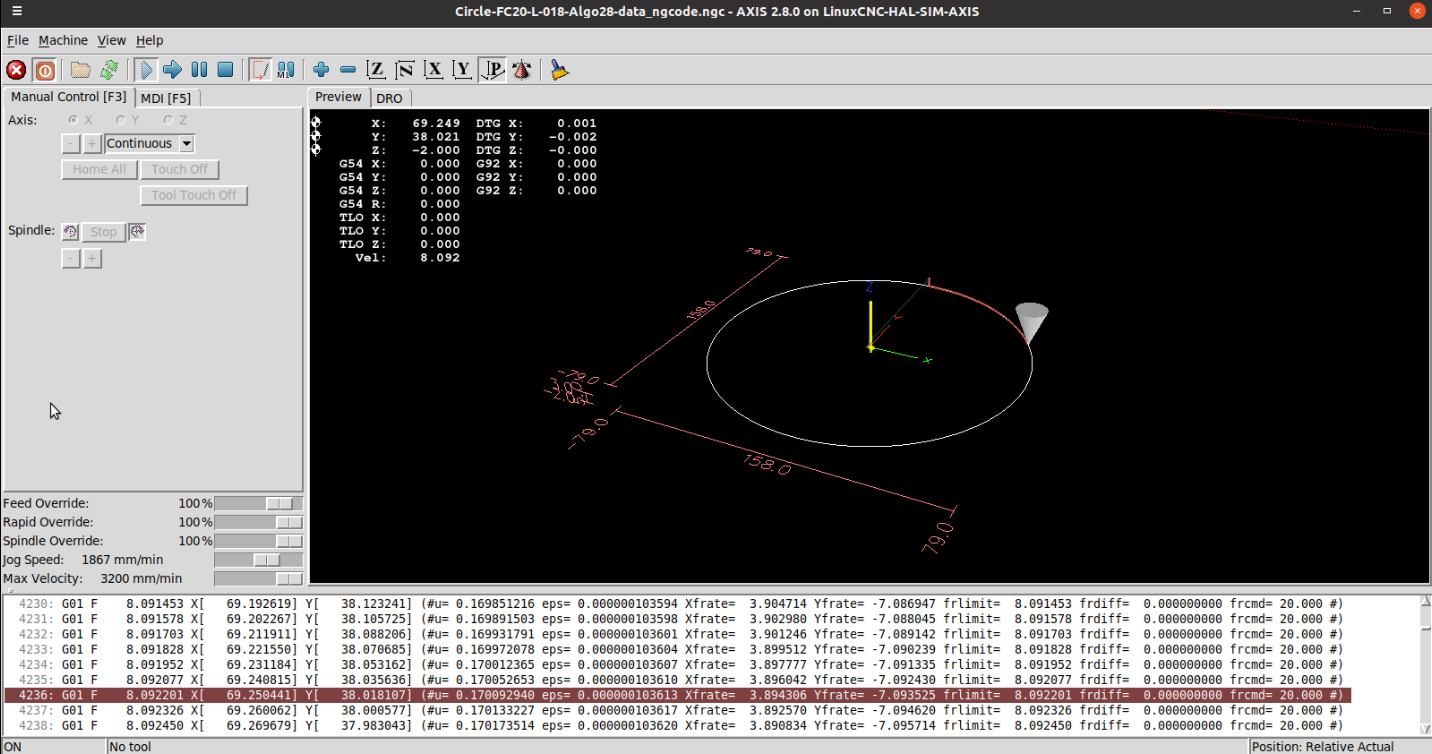
\includegraphics[width=1.65\textwidth]{Chap4/Validation/Circle/Circle-FC20-L-018-Algo28-CNC-Validation-Screenshot_2023-10-09_09-46-06.png} 
	\end{figure}
	
	
\end{landscape}

%% 2 ELLIPSE LINUXCNC
%% ==================================
\clearpage
\pagebreak
\begin{landscape}
	
	\begin{figure}
		\centering
		\caption  {Ellipse validation LinuxCNC-Axis execution}
		\label{img-Ellipse validation LinuxCNC-Axis execution}
		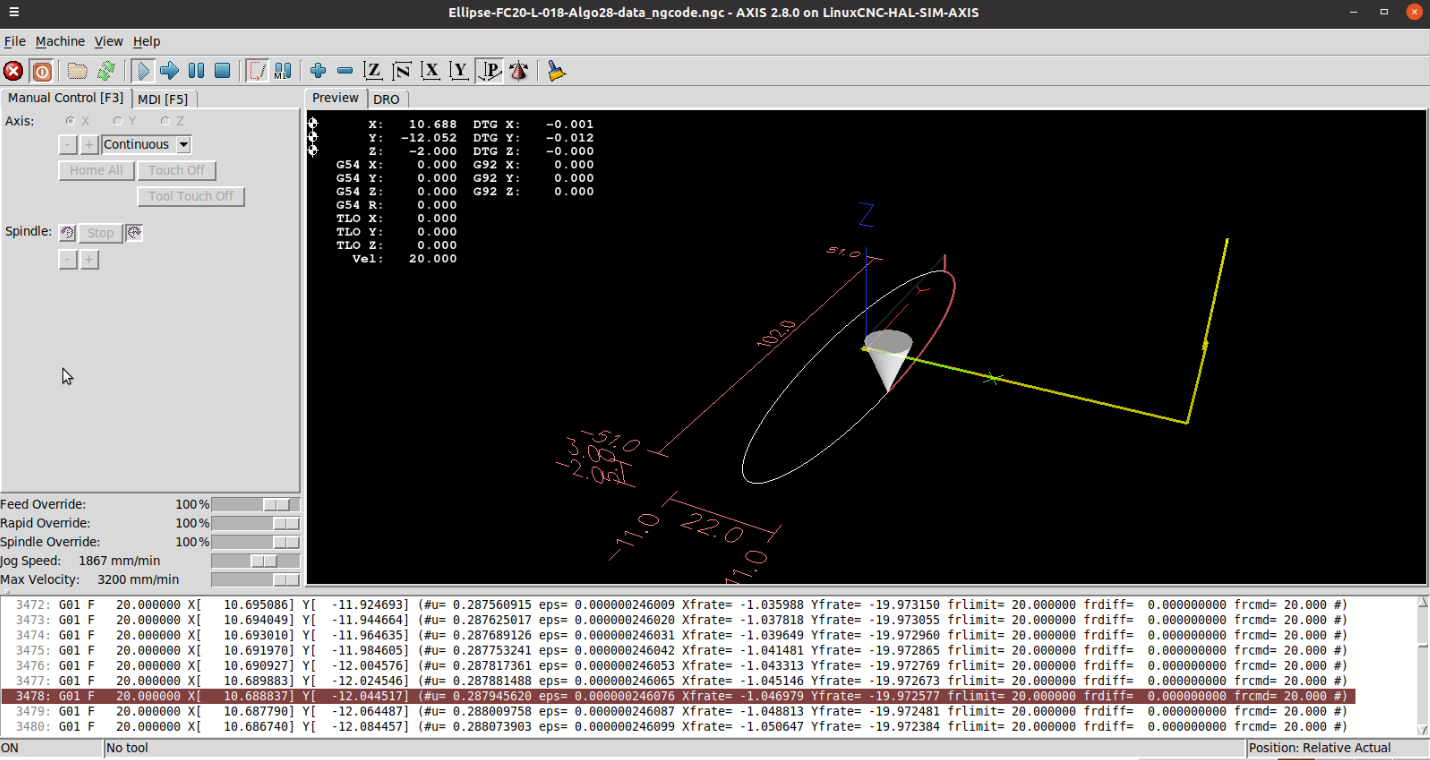
\includegraphics[width=1.65\textwidth]{Chap4/Validation/Ellipse/Ellipse-FC20-L-018-Algo28-CNC-Validation-Screenshot_2023-10-09_09-56-34.png} 
	\end{figure}
	
	
\end{landscape}

%% 3 TEARDROP LINUXCNC
%% ==================================
\clearpage
\pagebreak
\begin{landscape}
	
	\begin{figure}
		\centering
		\caption  {Teardrop validation LinuxCNC-Axis execution}
		\label{img-Teardrop validation LinuxCNC-Axis execution}
		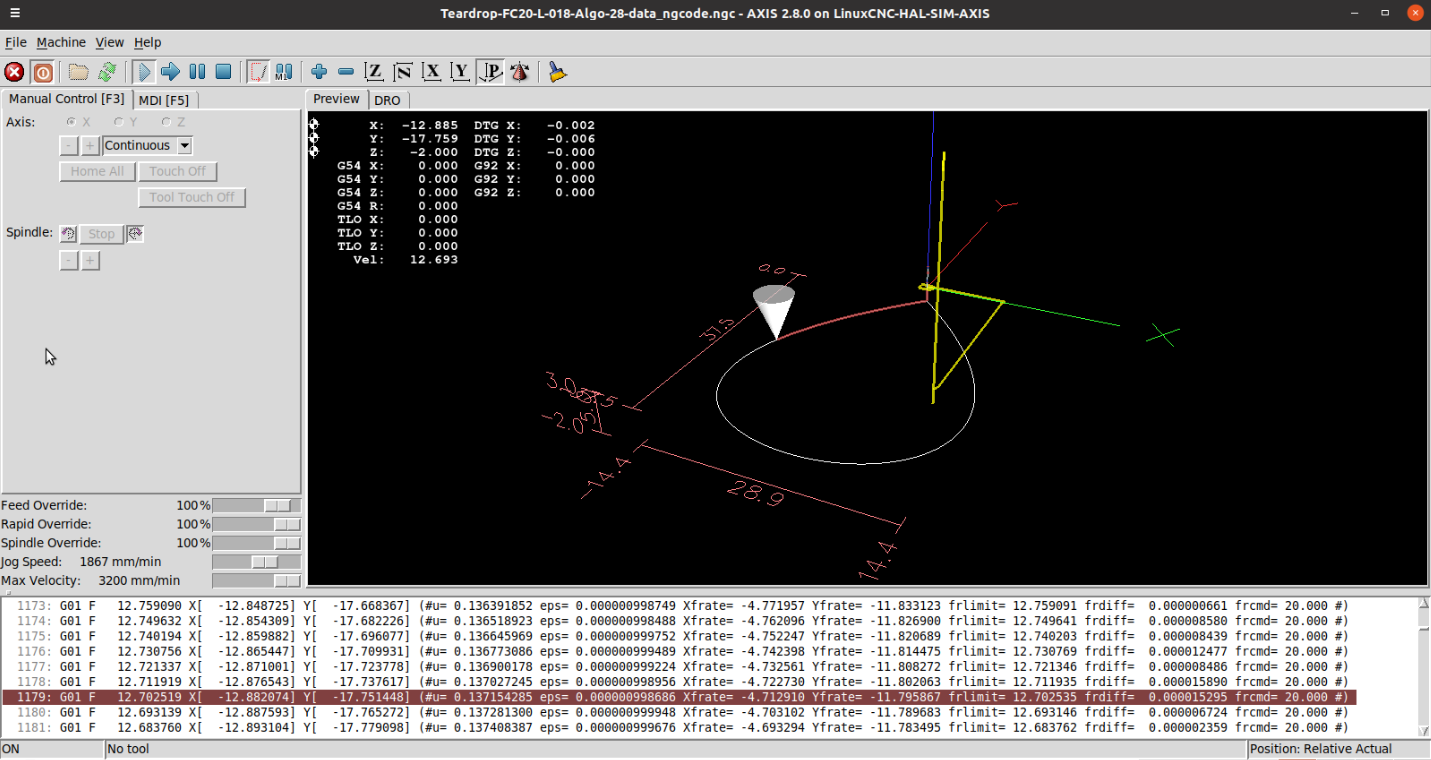
\includegraphics[width=1.65\textwidth]{Chap4/Validation/Teardrop/Teardrop-FC20-L-018-Algo28-CNC-Validation-Screenshot_2023-10-09_10-00-49.png} 
	\end{figure}
	
\end{landscape}

%% 4 BUTTERFLY LINUXCNC
%% ==================================
\clearpage
\pagebreak
\begin{landscape}
	
	\begin{figure}
		\centering
		\caption  {Butterfly validation LinuxCNC-Axis execution}
		\label{img-Butterfly validation LinuxCNC-Axis execution}
		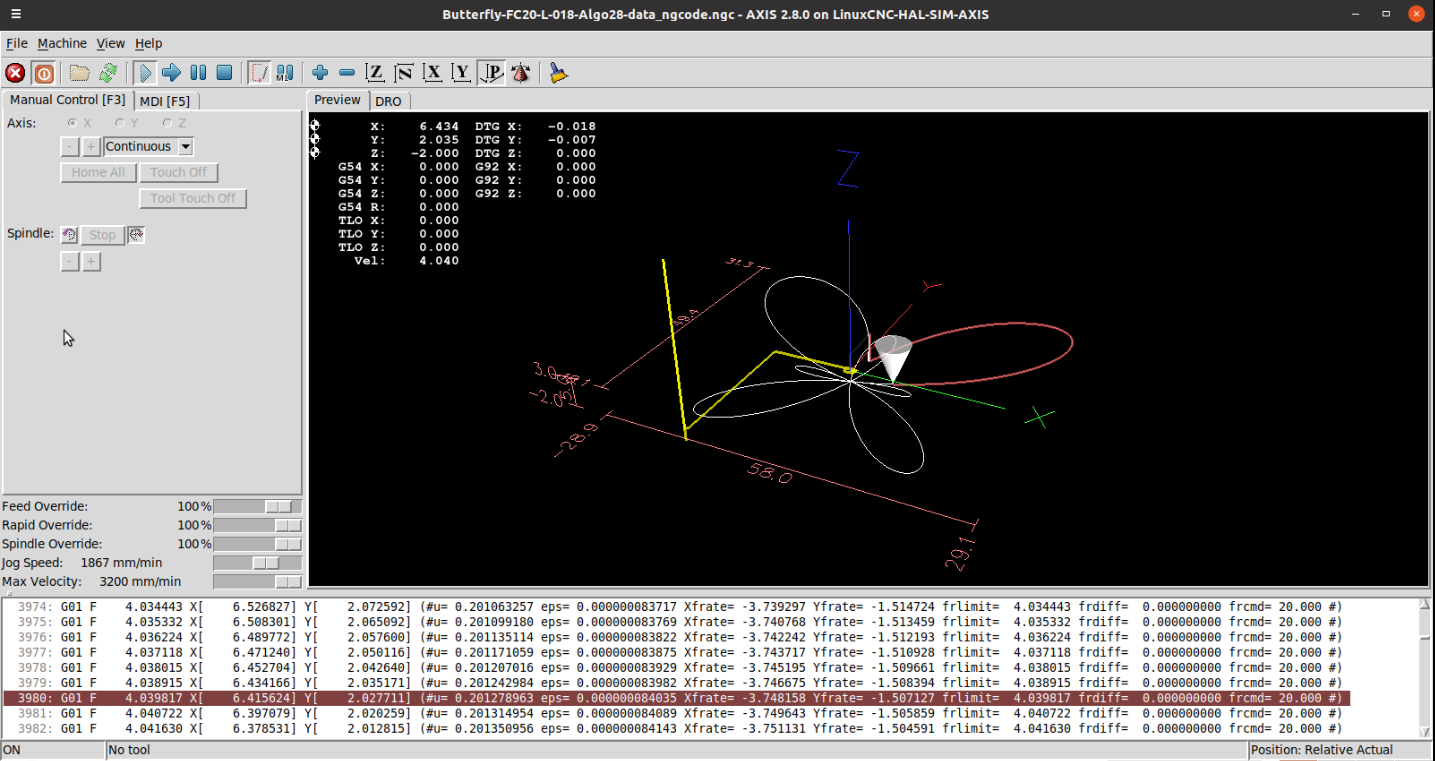
\includegraphics[width=1.65\textwidth]{Chap4/Validation/Butterfly/Butterfly-FC20-L-018-Algo28-CNC-Validation-Screenshot_2023-10-09_10-19-54.png} 
	\end{figure}	
	
\end{landscape}

%% 5 SNAILSHELL LINUXCNC
%% ==================================
\clearpage
\pagebreak
\begin{landscape}
	
	\begin{figure}
		\centering
		\caption  {Snailshell validation LinuxCNC-Axis execution}
		\label{img-Snailshell validation LinuxCNC-Axis execution}
		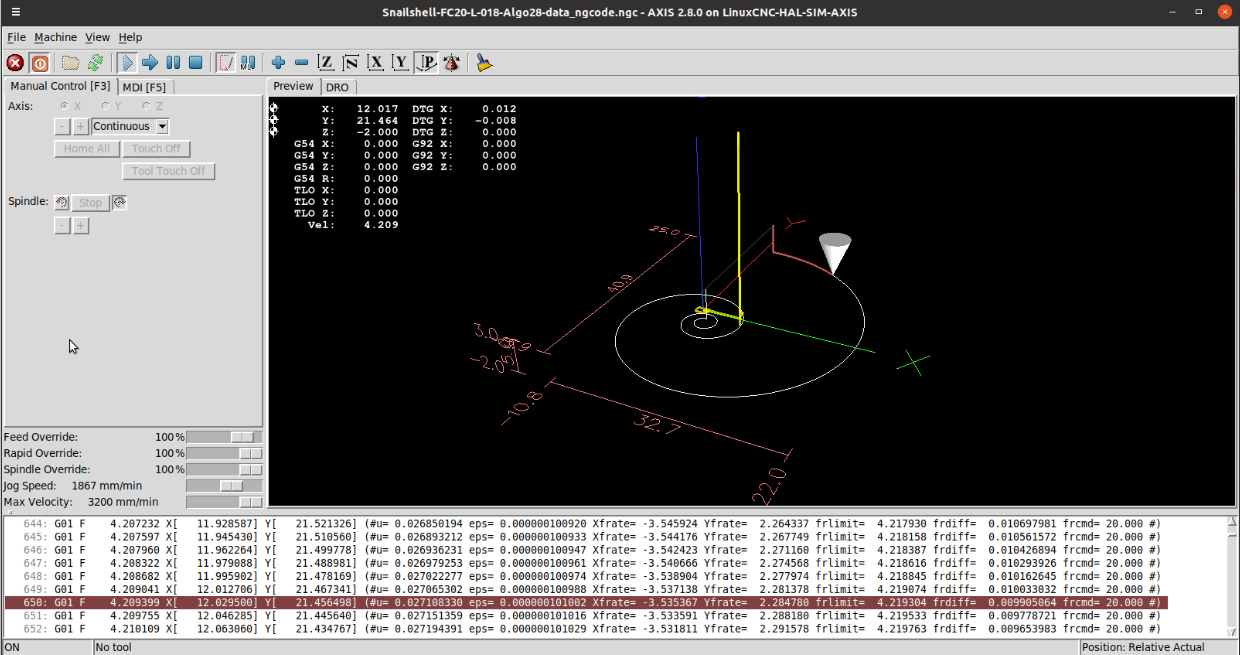
\includegraphics[width=1.65\textwidth]{Chap4/Validation/Snailshell/Snailshell-FC20-L-018-Algo28-CNC-Validation-Screenshot_2023-10-09_10-25-28.png} 
	\end{figure}	
	
\end{landscape}

%% 6 SKEWEED-ASTROID
%% ==================================
\clearpage
\pagebreak
\begin{landscape}
	
	\begin{figure}
		\centering
		\caption  {Skewed-Astroid validation LinuxCNC-Axis execution}
		\label{img-Skewed-Astroid validation LinuxCNC-Axis execution}
		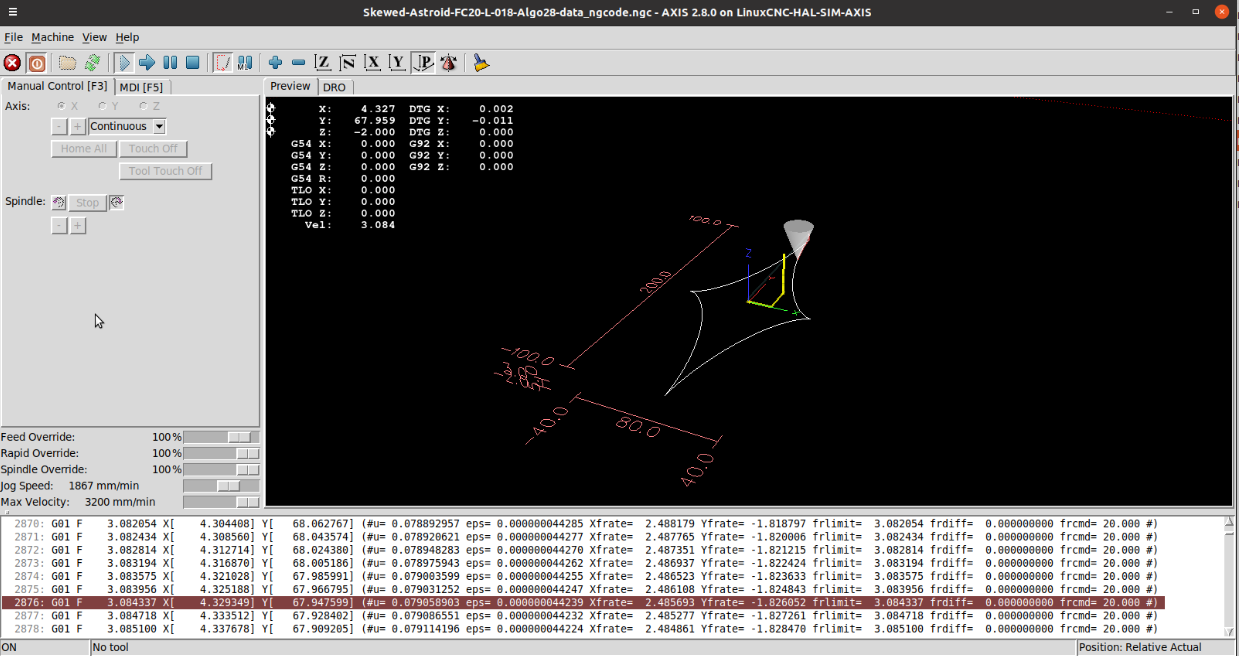
\includegraphics[width=1.65\textwidth]{Chap4/Validation/Skewed-Astroid/Skewed-Astroid-FC20-L-018-Algo28-CNC-Validation-Screenshot_2023-10-09_10-38-31.png} 
	\end{figure}	
	
\end{landscape}


%% 7 RIBBON-10L LINUXCNC
%% ==================================
\clearpage
\pagebreak
\begin{landscape}
	
	\begin{figure}
		\centering
		\caption  {Ribbon-10L validation LinuxCNC-Axis execution}
		\label{img-Ribbon-10L validation LinuxCNC-Axis execution}
		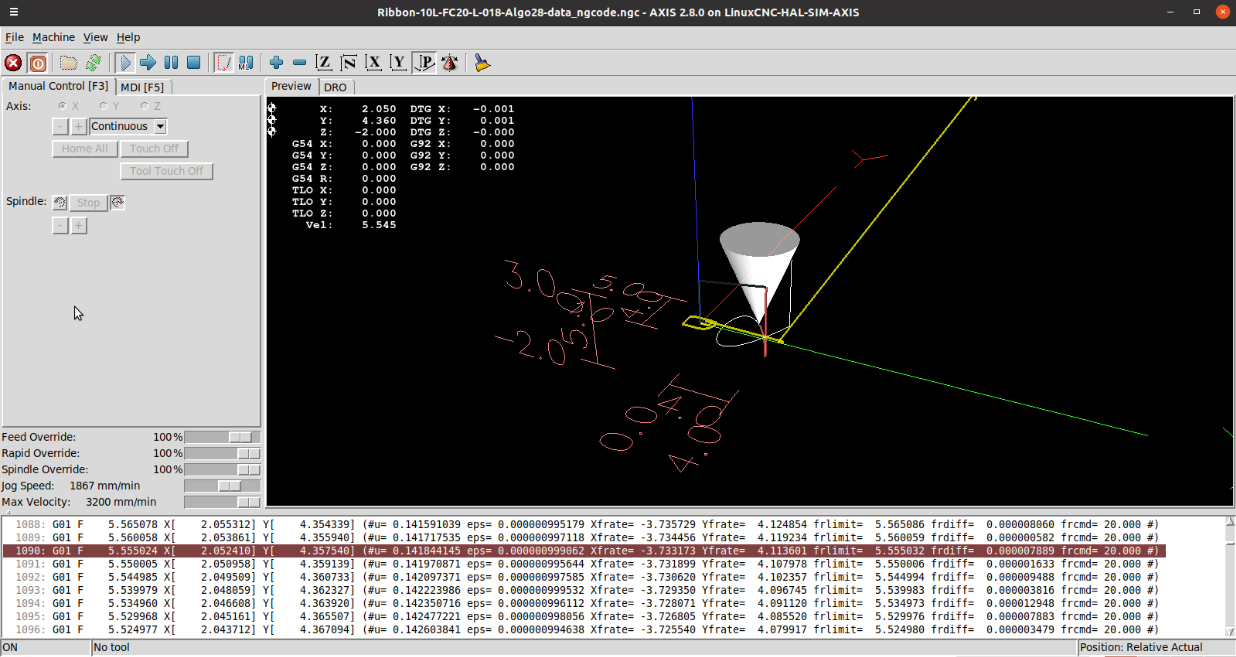
\includegraphics[width=1.65\textwidth]{Chap4/Validation/Ribbon-10L/Ribbon-10L-FC20-L-018-Algo28-CNC-Validation-Screenshot_2023-10-09_10-41-05.png} 
	\end{figure}	
	
\end{landscape}

%% 8 RIBBON-100 LINUXCNC
%% ==================================
\clearpage
\pagebreak
\begin{landscape}
	
	\begin{figure}
		\centering
		\caption  {Ribbon-100L validation LinuxCNC-Axis execution}
		\label{img-Ribbon-100L validation LinuxCNC-Axis execution}
		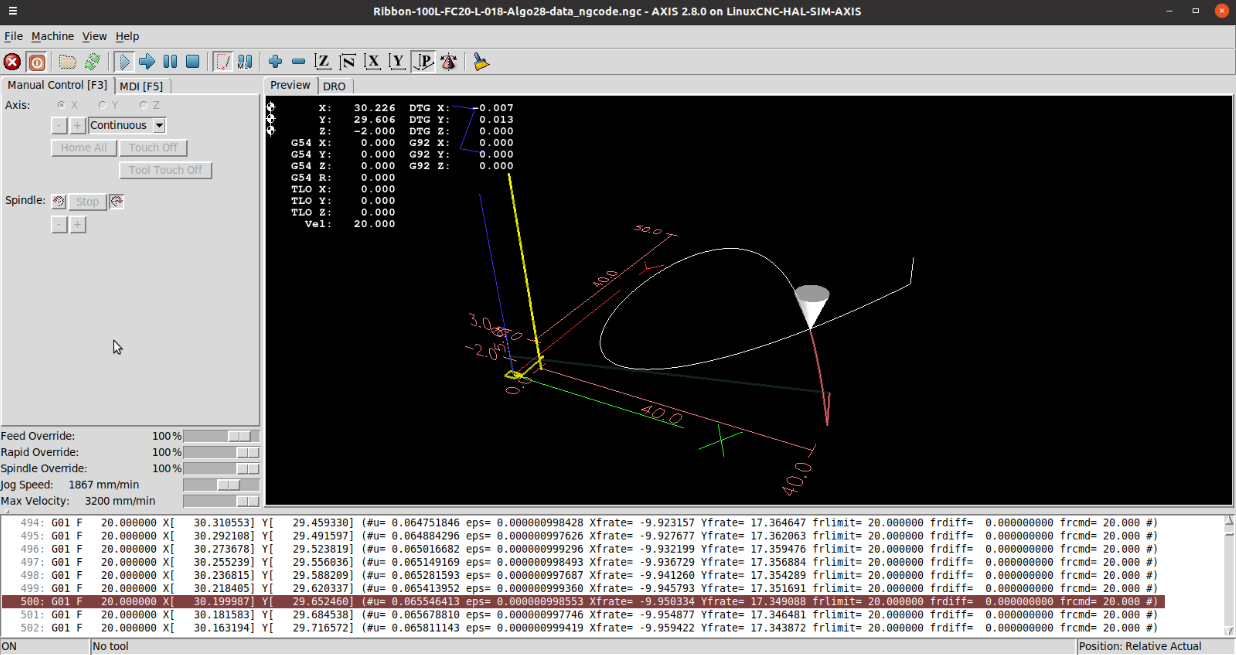
\includegraphics[width=1.65\textwidth]{Chap4/Validation/Ribbon-100L/Ribbon-100L-FC20-L-018-Algo28-CNC-Validation-Screenshot_2023-10-09_10-45-00.png} 
	\end{figure}	
	
\end{landscape}


%% 9 ASTEPI LINUXCNC
%% ==================================
\clearpage
\pagebreak
\begin{landscape}
	
	\begin{figure}
		\centering
		\caption  {AstEpi validation LinuxCNC-Axis execution}
		\label{img-AstEpi validation LinuxCNC-Axis execution} 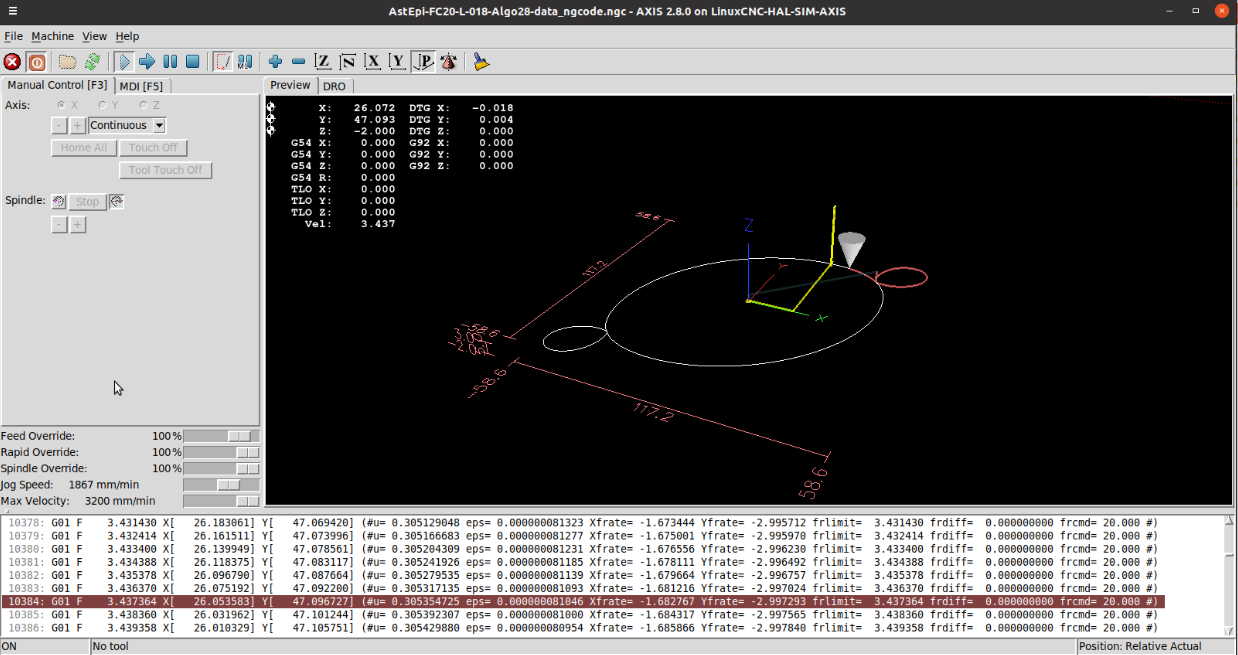
\includegraphics[width=1.65\textwidth]{Chap4/Validation/AstEpi/AstEpi-FC20-L-018-Algo28-CNC-Validation-Screenshot_2023-10-09_11-01-23.png} 
	\end{figure}
	
\end{landscape}

%% 10 SHAHYP LINUXCNC
%% ==================================
\clearpage
\pagebreak
\begin{landscape}
	
	\begin{figure}
		\centering
		\caption  {SnaHyp validation LinuxCNC-Axis execution}
		\label{img-SnaHyp validation LinuxCNC-Axis execution} 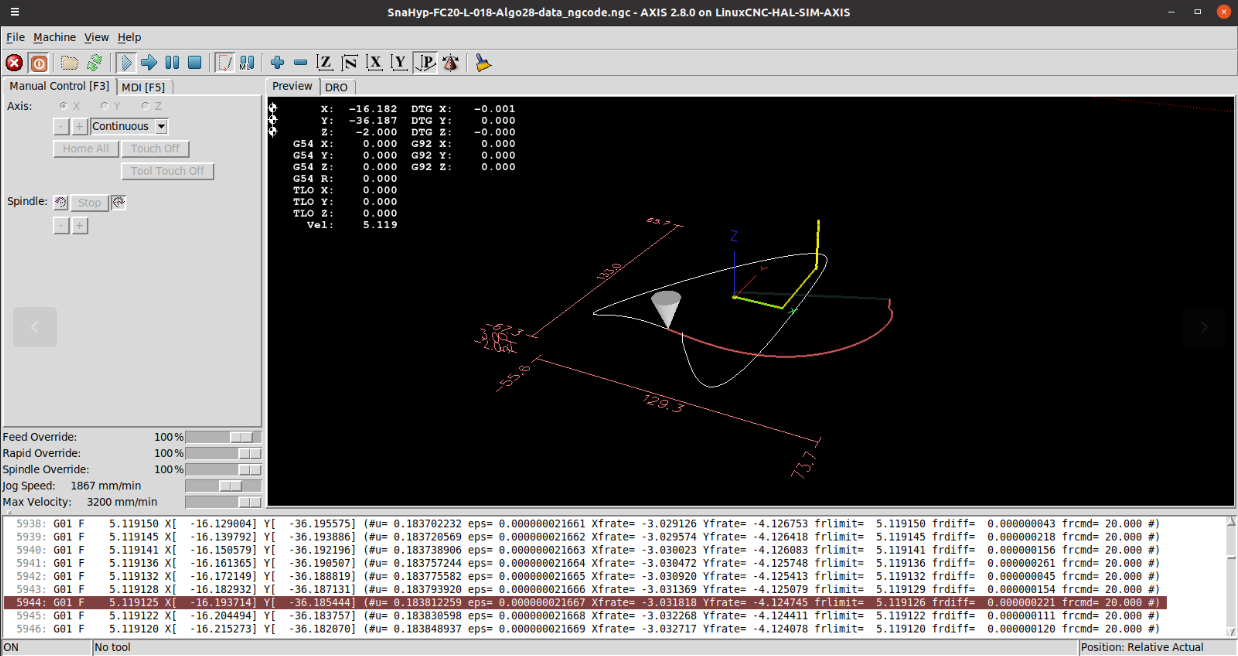
\includegraphics[width=1.65\textwidth]{Chap4/Validation/SnaHyp/SnaHyp-FC20-L-018-Algo28-CNC-Validation-Screenshot_2023-10-09_11-30-38.png} 
	\end{figure}
	
\end{landscape}

\clearpage
\pagebreak

\section{\textbf{APPENDIX CIRCLE CURVE}} \label{APPENDIX CIRCLE CURVE}

\subsection       {Plot of Circle curve
[\ref      {01-img-Plot of Circle curve.pdf} ] }
\label{ssec-01-img-Plot of Circle curve.pdf}

\subsection       {Circle Radius of Curvature
[\ref      {02-img-Circle Radius of Curvature.pdf}] }
\label{ssec-02-img-Circle Radius of Curvature.pdf}

\subsection       {Circle Validation in LinuxCNC
[\ref      {03-img-Circle-Validation-in-LinuxCNC.png} ] }
\label{ssec-03-img-Circle-Validation-in-LinuxCNC.png}

\subsection     {Circle Direction of Travel 3D
[\ref      {04-img-Circle Direction of Travel 3D.pdf} ] }
\label{ssec-04-img-Circle Direction of Travel 3D.pdf}

\subsection       {Circle First and Second Order Taylor's Approx
[\ref      {05-img-Circle-First-and-Second-Order-Taylors-Approx.pdf}] }
\label{ssec-05-img-Circle-First-and-Second-Order-Taylors-Approx.pdf}

\subsection       {Circle First minus Second Order Taylor's Approx
[\ref      {06-img-Circle-First-minus-Second-Order-Taylors-Approx.pdf}] }
\label{ssec-06-img-Circle-First-minus-Second-Order-Taylors-Approx.pdf}

\subsection       {Circle Separate First and Second Order Taylor's Approx
[\ref      {07-img-Circle-Separation-First-and-Second-Order-Taylors-Approx.pdf} ] }
\label{ssec-07-img-Circle-Separation-First-and-Second-Order-Taylors-Approx.pdf}

\subsection       {Circle Separation SAL and SCL
[\ref      {08-img-Circle-Separation-SAL-and-SCL.pdf}] }
\label{ssec-08-img-Circle-Separation-SAL-and-SCL.pdf}

\subsection       {Circle Chord-error in close view 2 scales
[\ref      {09-img-Circle-Chord-error-in-close-view-2-scales.pdf}] }
\label{ssec-09-img-Circle-Chord-error-in-close-view-2-scales.pdf}

\subsection       {Circle Four Components Feedrate Limit
[\ref      {10-img-Circle-Four-Components-Feedrate-Limit.pdf} ] }
\label{ssec-10-img-Circle-Four-Components-Feedrate-Limit.pdf}

\subsection    {Circle FrateCommand FrateLimit and Curr-Frate
[\ref      {11-img-Circle-FrateCommand-FrateLimit-and-Curr-Frate.pdf}] }
\label{ssec-11-img-Circle-FrateCommand-FrateLimit-and-Curr-Frate.pdf}

\subsection     {Circle FeedRateLimit minus CurrFeedRate
[\ref      {12-img-Circle-FeedRateLimit-minus-CurrFeedRate.pdf} ] }
\label{ssec-12-img-Circle-FeedRateLimit-minus-CurrFeedRate.pdf}

\subsection     {Circle FC20-Nominal X and Y Feedrate Profiles
[\ref      {13-img-Circle-FC20-Nominal-X-and-Y-Feedrate-Profiles.pdf} ] }
\label{ssec-13-img-Circle-FC20-Nominal-X-and-Y-Feedrate-Profiles.pdf}

\subsection     {Circle FC20 Nominal Tangential Acceleration
[\ref      {14-img-Circle-FC20-Nominal-Tangential-Acceleration.pdf} ] }
\label{ssec-14-img-Circle-FC20-Nominal-Tangential-Acceleration.pdf}

\subsection     {Circle FC20 Nominal Rising S-Curve Profile
[\ref      {15-img-Circle-FC20-Nominal-Rising-S-Curve-Profile.pdf} ] }
\label{ssec-15-img-Circle-FC20-Nominal-Rising-S-Curve-Profile.pdf}

\subsection     {Circle FC20 Nominal Falling S-Curve Profile
[\ref      {16-img-Circle-FC20-Nominal-Falling-S-Curve-Profile.pdf}] }
\label{ssec-16-img-Circle-FC20-Nominal-Falling-S-Curve-Profile.pdf}

\subsection       {Circle FC10 Colored Feedrate Profile data ngcode
[\ref      {17-img-Circle-FC10-Colored-Feedrate-Profile-data_ngcode.png} ] }
\label{ssec-17-img-Circle-FC10-Colored-Feedrate-Profile-data_ngcode.png}

\subsection       {Circle FC20 Colored Feedrate Profile data ngcode
[\ref      {18-img-Circle-FC20-Colored-Feedrate-Profile-data_ngcode.png} ] }
\label{ssec-18-img-Circle-FC20-Colored-Feedrate-Profile-data_ngcode.png}

Continue ...\\

\subsection       {Circle FC30 Colored Feedrate Profile data ngcode
[\ref      {19-img-Circle-FC30-Colored-Feedrate-Profile-data_ngcode.png} ] }
\label{ssec-19-img-Circle-FC30-Colored-Feedrate-Profile-data_ngcode.png}

\subsection       {Circle FC40 Colored Feedrate Profile data ngcode
[\ref      {20-img-Circle-FC40-Colored-Feedrate-Profile-data_ngcode.png} ] }
\label{ssec-20-img-Circle-FC40-Colored-Feedrate-Profile-data_ngcode.png}

\subsection       {Circle FC10 Tangential Acceleration
[\ref      {21-img-Circle-FC10-Tangential-Acceleration.pdf}] }
\label{ssec-21-img-Circle-FC10-Tangential-Acceleration.pdf}

\subsection       {Circle FC20 Tangential Acceleration
[\ref      {22-img-Circle-FC20-Tangential-Acceleration.pdf}] }
\label{ssec-22-img-Circle-FC20-Tangential-Acceleration.pdf}

\subsection       {Circle FC30 Tangential Acceleration
[\ref      {23-img-Circle-FC30-Tangential-Acceleration.pdf}] }
\label{ssec-23-img-Circle-FC30-Tangential-Acceleration.pdf}

\subsection       {Circle FC40 Tangential Acceleration
[\ref      {24-img-Circle-FC40-Tangential-Acceleration.pdf}] }
\label{ssec-24-img-Circle-FC40-Tangential-Acceleration.pdf}

\subsection       {Circle FC20 Nominal Separation NAL and NCL
[\ref      {25-img-Circle-FC20-Nominal-Separation-NAL-and-NCL.pdf}] }
\label{ssec-25-img-Circle-FC20-Nominal-Separation-NAL-and-NCL.pdf}

\subsection       {Circle SAL minus SCL for FC10 FC20 FC30 FC40
[\ref      {26-img-Circle-Difference-SAL-minus-SCL-for-FC10-FC20-FC30-FC40.pdf}] }
\label{ssec-26-img-Circle-Difference-SAL-minus-SCL-for-FC10-FC20-FC30-FC40.pdf}


\subsection       {Circle FC10 FrateCmd CurrFrate X-Frate Y-Frate
[\ref      {27-img-Circle-FC10-FrateCmd-CurrFrate-X-Frate-Y-Frate.pdf}] }
\label{ssec-27-img-Circle-FC10-FrateCmd-CurrFrate-X-Frate-Y-Frate.pdf}

\subsection       {Circle FC20 FrateCmd CurrFrate X-Frate Y-Frate
[\ref      {28-img-Circle-FC20-FrateCmd-CurrFrate-X-Frate-Y-Frate.pdf}] }
\label{ssec-28-img-Circle-FC20-FrateCmd-CurrFrate-X-Frate-Y-Frate.pdf}

\subsection       {Circle FC30 FrateCmd CurrFrate X-Frate Y-Frate
[\ref      {29-img-Circle-FC30-FrateCmd-CurrFrate-X-Frate-Y-Frate.pdf}] }
\label{ssec-29-img-Circle-FC30-FrateCmd-CurrFrate-X-Frate-Y-Frate.pdf}

\subsection       {Circle FC40 FrateCmd CurrFrate X-Frate Y-Frate
[\ref      {30-img-Circle-FC40-FrateCmd-CurrFrate-X-Frate-Y-Frate.pdf}] }
\label{ssec-30-img-Circle-FC40-FrateCmd-CurrFrate-X-Frate-Y-Frate.pdf}

\subsection       {Circle FC10 Four Components FeedrateLimit
[\ref      {31-img-Circle-FC10-Four-Components-FeedrateLimit.pdf}] }
\label{ssec-31-img-Circle-FC10-Four-Components-FeedrateLimit.pdf}

\subsection       {Circle FC20 Four Components FeedrateLimit
[\ref      {32-img-Circle-FC20-Four-Components-FeedrateLimit.pdf}] }
\label{ssec-32-img-Circle-FC20-Four-Components-FeedrateLimit.pdf}

\subsection       {Circle FC30 Four Components FeedrateLimit
[\ref      {33-img-Circle-FC30-Four-Components-FeedrateLimit.pdf}] }
\label{ssec-33-img-Circle-FC30-Four-Components-FeedrateLimit.pdf}

\subsection       {Circle FC40 Four Components FeedrateLimit
[\ref      {34-img-Circle-FC40-Four-Components-FeedrateLimit.pdf}]}
\label{ssec-34-img-Circle-FC40-Four-Components-FeedrateLimit.pdf}

\subsection       {Circle Histogram Points FC10 FC20 FC30 FC40
[\ref       {35-img-Circle-Histogram-Points-FC10-FC20-FC30-FC40.pdf}] }
\label{ssec-35-img-Circle-Histogram-Points-FC10-FC20-FC30-FC40.pdf}

\subsection    {Circle Table distribution of interpolated points
[\ref      {tab-Circle Table distribution of interpolated points}] }
\label{ssec-tab-Circle Table distribution of interpolated points}

\subsection          {Circle Table FC10-20-30-40 Run Performance data
[\ref       {tab-app4-Circle-Table-FC10-20-30-40-Run-Performance-data} ] }
\label{ssec-tab-app4-Circle-Table-FC10-20-30-40-Run-Performance-data}


%% =====================================================
%% ==================================================
\clearpage
\pagebreak

\begin{figure}
	\caption     {Plot of Circle curve}
	\label{01-img-Plot of Circle curve.pdf}
	%%	\centering
	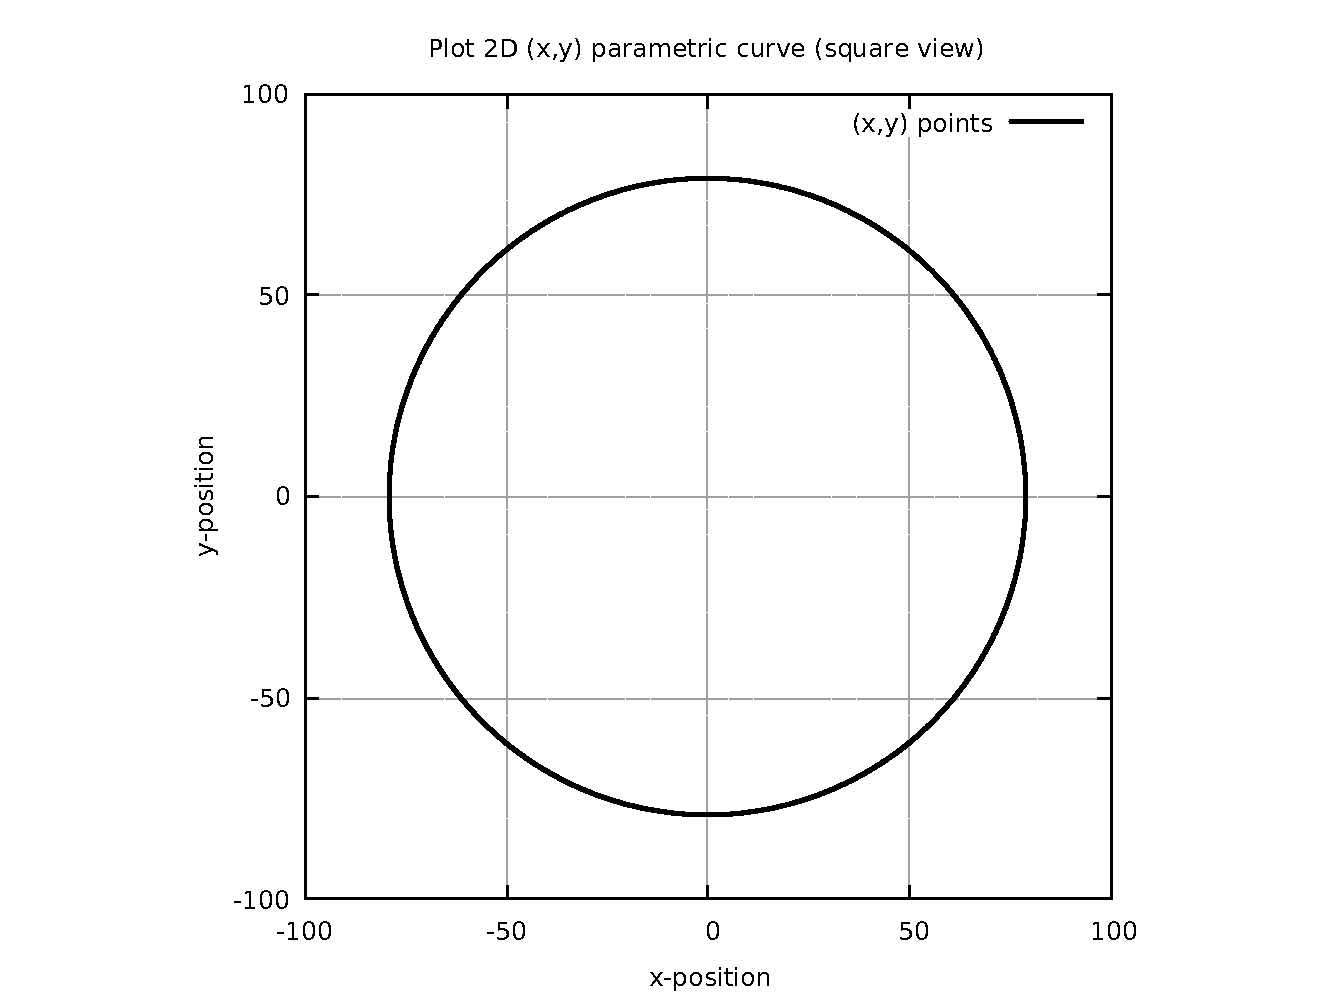
\includegraphics[width=1.00\textwidth]{Chap4/appendix/app-Circle/plots/01-img-Plot of Circle curve.pdf}
\end{figure}	


\begin{figure}
	\caption     {Circle Radius of Curvature}
	\label{02-img-Circle Radius of Curvature.pdf}
	%%	\centering
	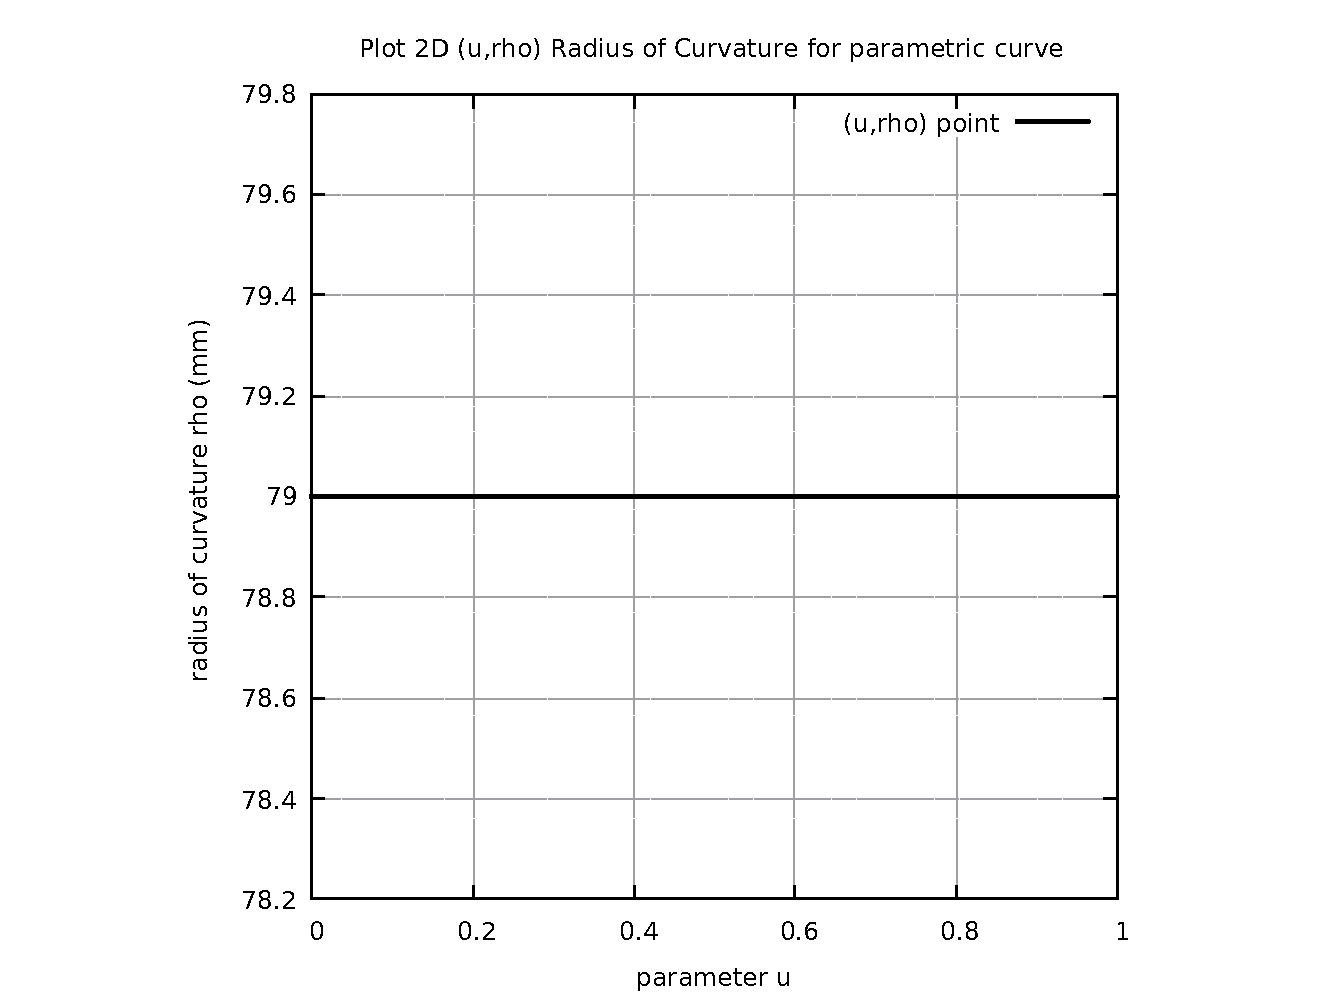
\includegraphics[width=1.00\textwidth]{Chap4/appendix/app-Circle/plots/02-img-Circle Radius of Curvature.pdf} 
\end{figure}	


%% ==================================================
\clearpage
\pagebreak

\begin{figure}
	\caption     {Circle Validation in LinuxCNC}
	\label{03-img-Circle-Validation-in-LinuxCNC.png}
	%%	\centering
	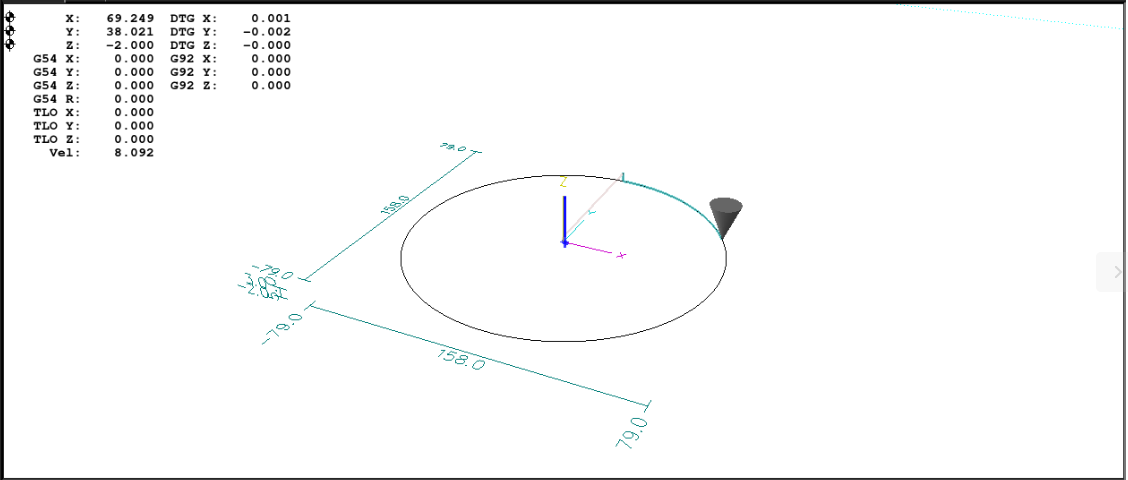
\includegraphics[width=1.00\textwidth]{Chap4/appendix/app-Circle/plots/03-img-Circle-Validation-in-LinuxCNC.png}
\end{figure}


\begin{figure}
	\caption     {Circle Direction of Travel 3D}
	\label{04-img-Circle Direction of Travel 3D.pdf}
	%%	\centering
	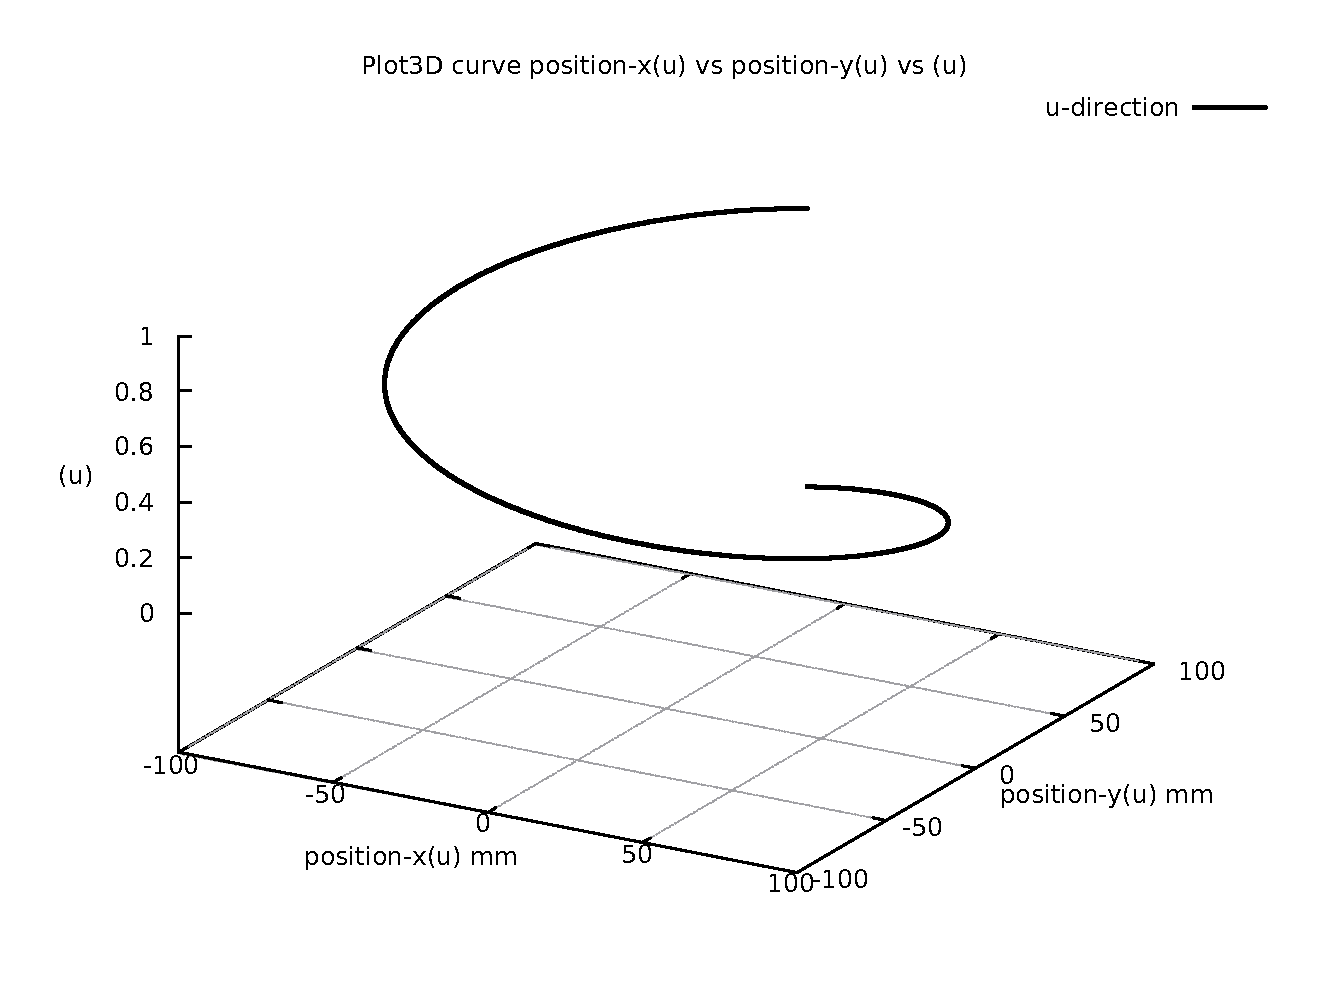
\includegraphics[width=1.00\textwidth]{Chap4/appendix/app-Circle/plots/04-img-Circle Direction of Travel 3D.pdf}
\end{figure}

%% ==================================================
\clearpage
\pagebreak

\begin{figure}
	\caption     {Circle First and Second Order Taylor's Approximation}
	\label{05-img-Circle-First-and-Second-Order-Taylors-Approx.pdf}
	%%	\centering
	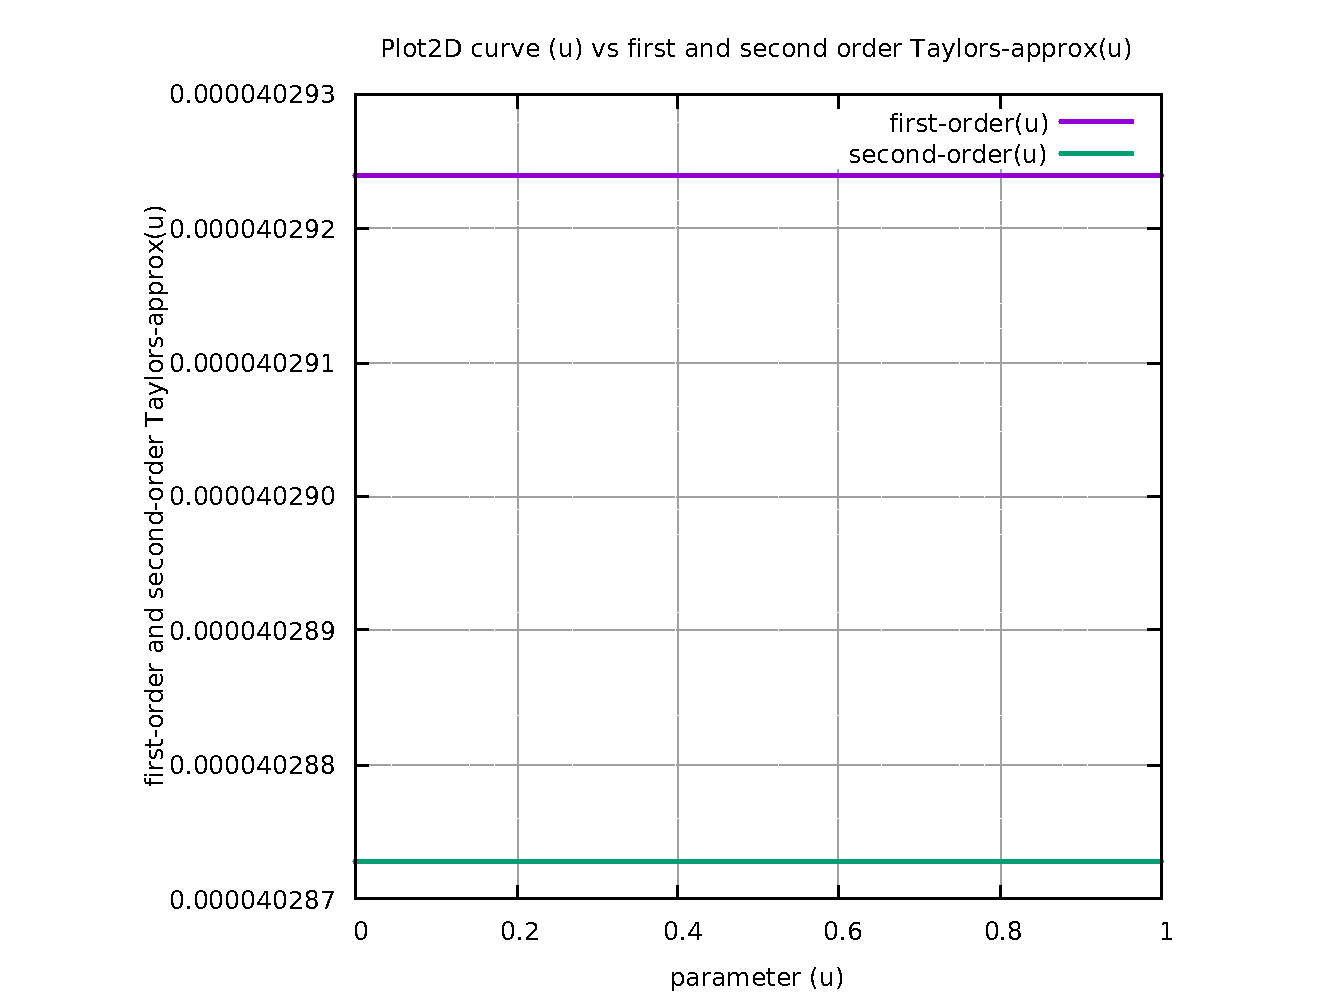
\includegraphics[width=1.00\textwidth]{Chap4/appendix/app-Circle/plots/05-img-Circle-First-and-Second-Order-Taylors-Approx.pdf}
\end{figure}


\begin{figure}
	\caption     {Circle First minus Second Order Taylor's Approximation}
	\label{06-img-Circle-First-minus-Second-Order-Taylors-Approx.pdf}
	%%	\centering
	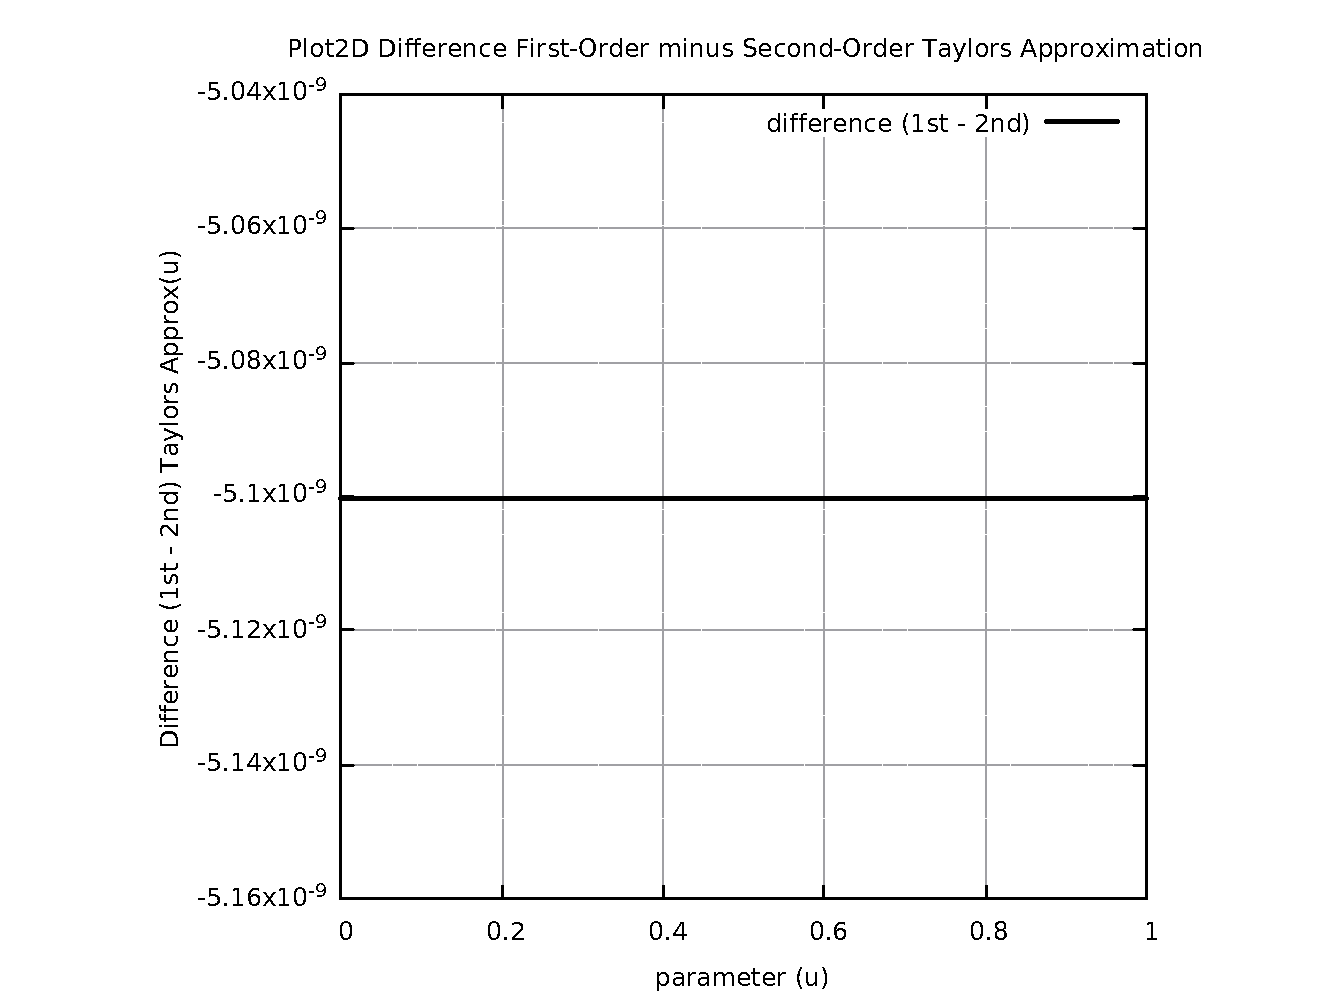
\includegraphics[width=1.00\textwidth]{Chap4/appendix/app-Circle/plots/06-img-Circle-First-minus-Second-Order-Taylors-Approx.pdf}
\end{figure}

%% ==================================================
\clearpage
\pagebreak

\begin{figure}
	\caption     {Circle Separation First and Second Order Taylor's Approximation}
	\label{07-img-Circle-Separation-First-and-Second-Order-Taylors-Approx.pdf}
	%%	\centering
	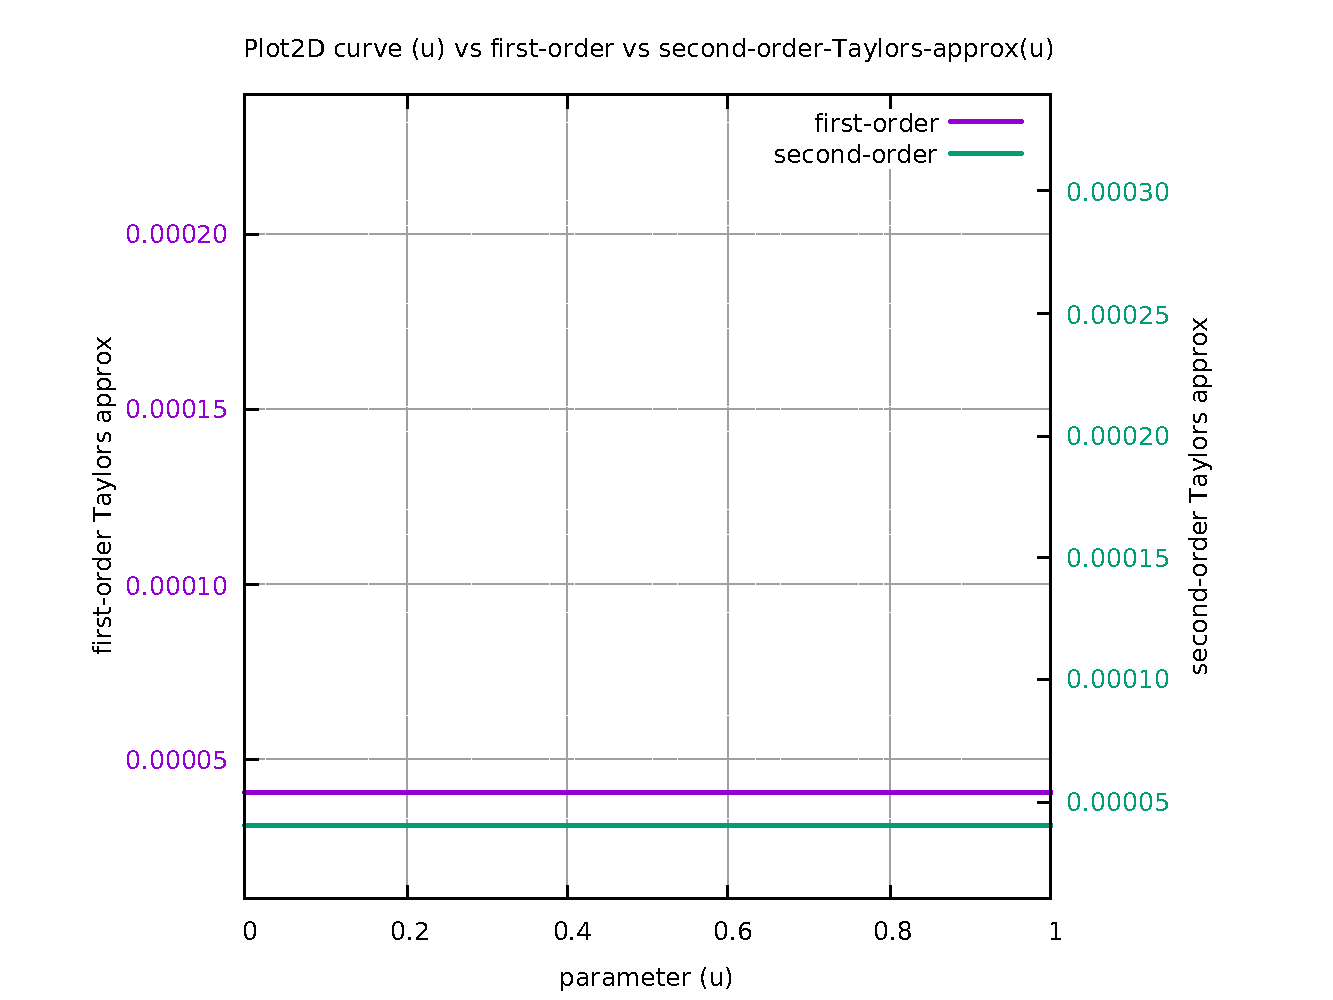
\includegraphics[width=1.00\textwidth]{Chap4/appendix/app-Circle/plots/07-img-Circle-Separation-First-and-Second-Order-Taylors-Approx.pdf}
\end{figure}


\begin{figure}
	\caption     {Circle Separation SAL and SCL}
	\label{08-img-Circle-Separation-SAL-and-SCL.pdf}
	%%	\centering
	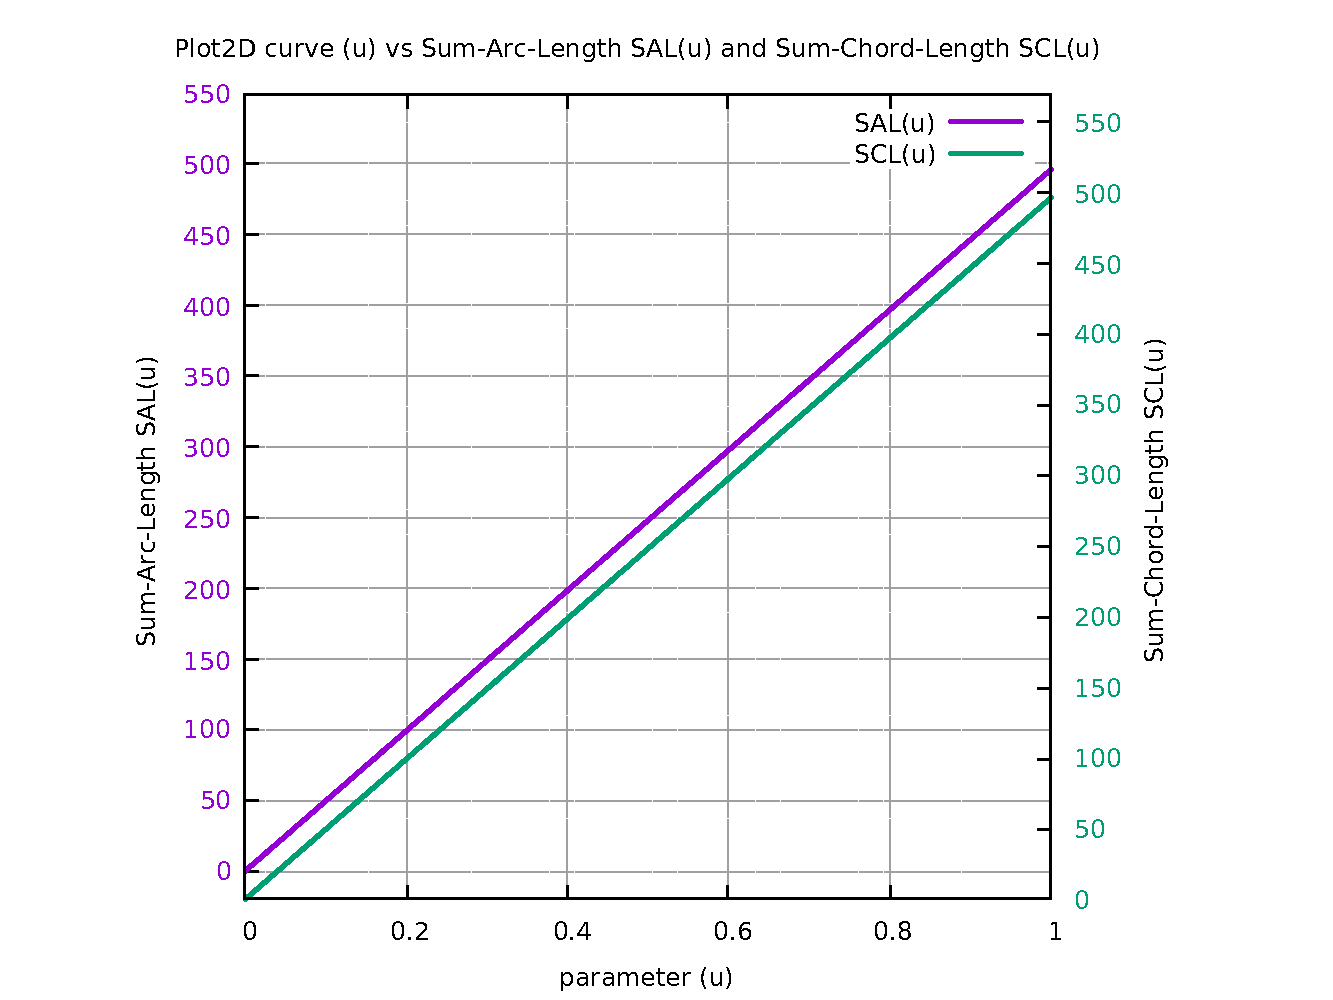
\includegraphics[width=1.00\textwidth]{Chap4/appendix/app-Circle/plots/08-img-Circle-Separation-SAL-and-SCL.pdf}
\end{figure}

%% ==================================================
\clearpage
\pagebreak

\begin{figure}
	\caption     {Circle Chord-error in close view 2 scales}
	\label{09-img-Circle-Chord-error-in-close-view-2-scales.pdf}
	%%	\centering
	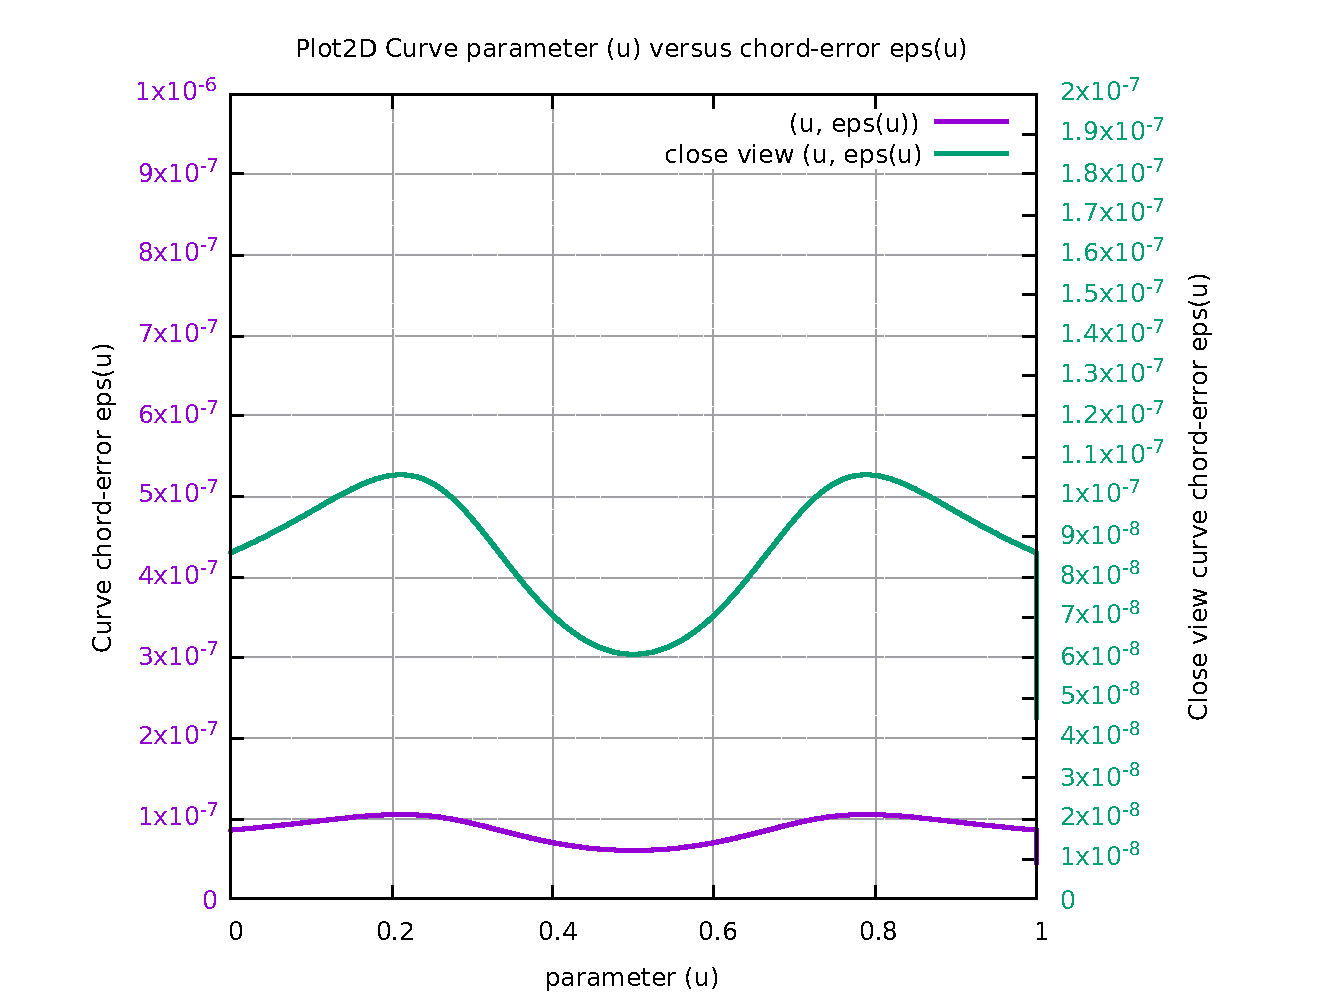
\includegraphics[width=1.00\textwidth]{Chap4/appendix/app-Circle/plots/09-img-Circle-Chord-error-in-close-view-2-scales.pdf}
\end{figure}


\begin{figure}
	\caption     {Circle Four Components Feedrate Limit}
	\label{10-img-Circle-Four-Components-Feedrate-Limit.pdf}
	%%	\centering
	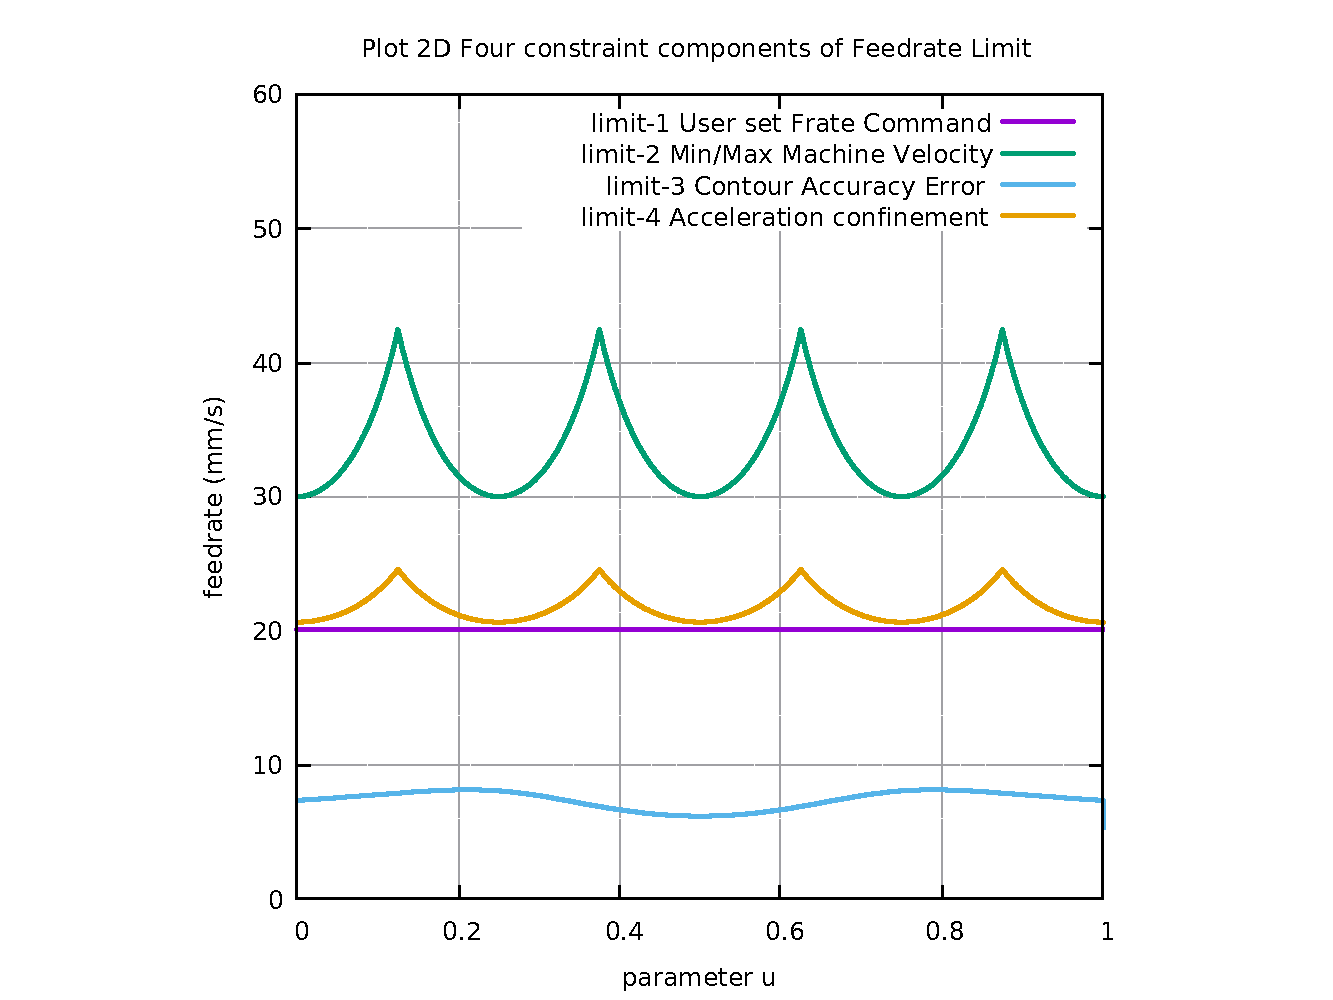
\includegraphics[width=1.00\textwidth]{Chap4/appendix/app-Circle/plots/10-img-Circle-Four-Components-Feedrate-Limit.pdf}
\end{figure}

%% ==================================================
\clearpage
\pagebreak

\begin{figure}
	\caption     {Circle FrateCommand FrateLimit and Curr-Frate}
	\label{11-img-Circle-FrateCommand-FrateLimit-and-Curr-Frate.pdf}
	%%	\centering
	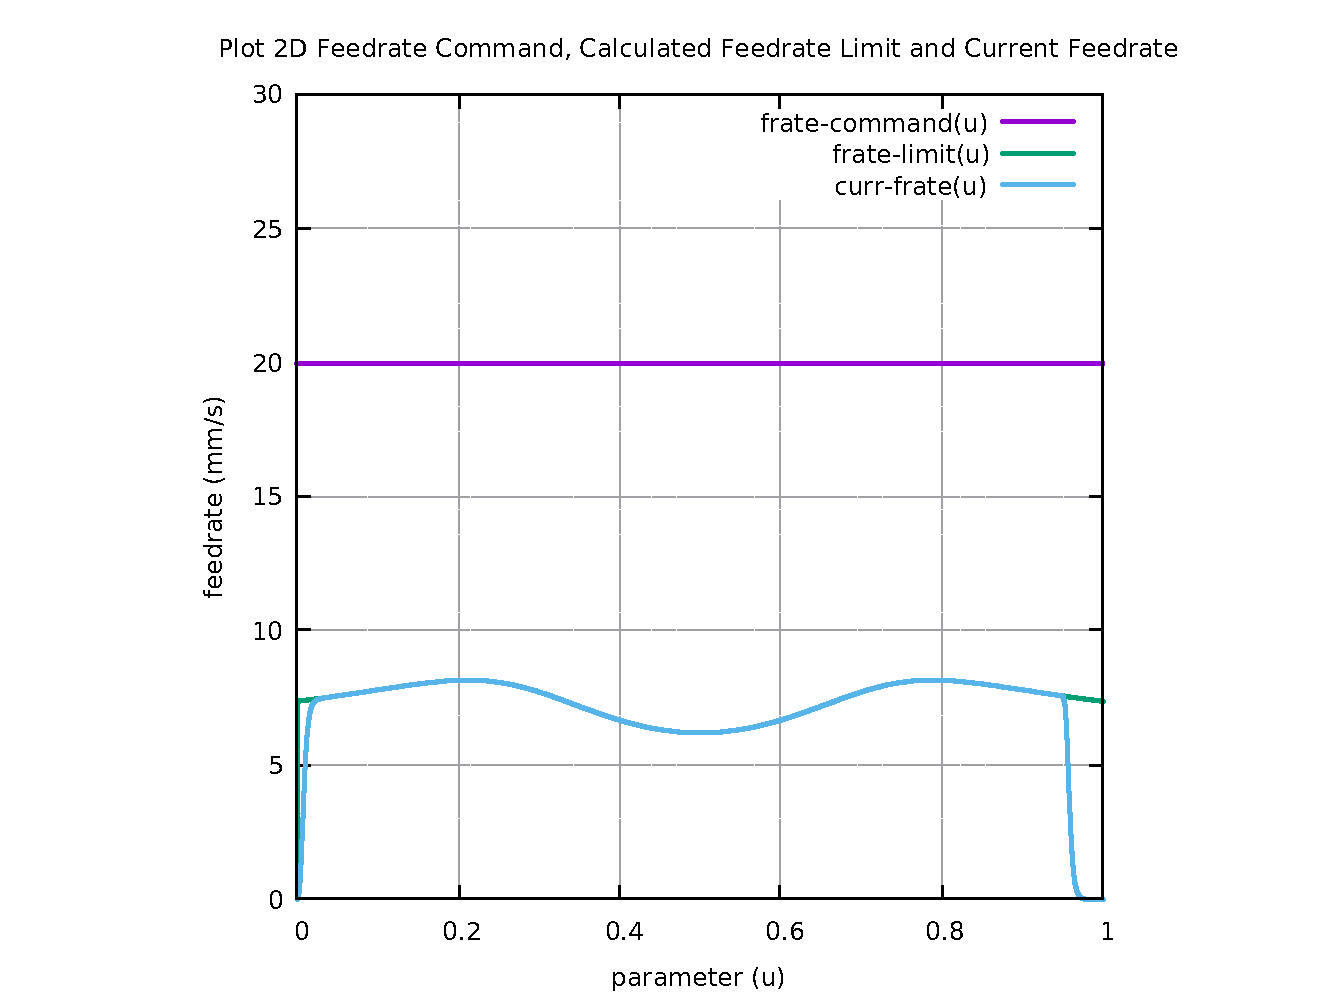
\includegraphics[width=1.00\textwidth]{Chap4/appendix/app-Circle/plots/11-img-Circle-FrateCommand-FrateLimit-and-Curr-Frate.pdf}
\end{figure}


\begin{figure}
	\caption     {Circle FeedRateLimit minus CurrFeedRate}
	\label{12-img-Circle-FeedRateLimit-minus-CurrFeedRate.pdf}
	%%	\centering
	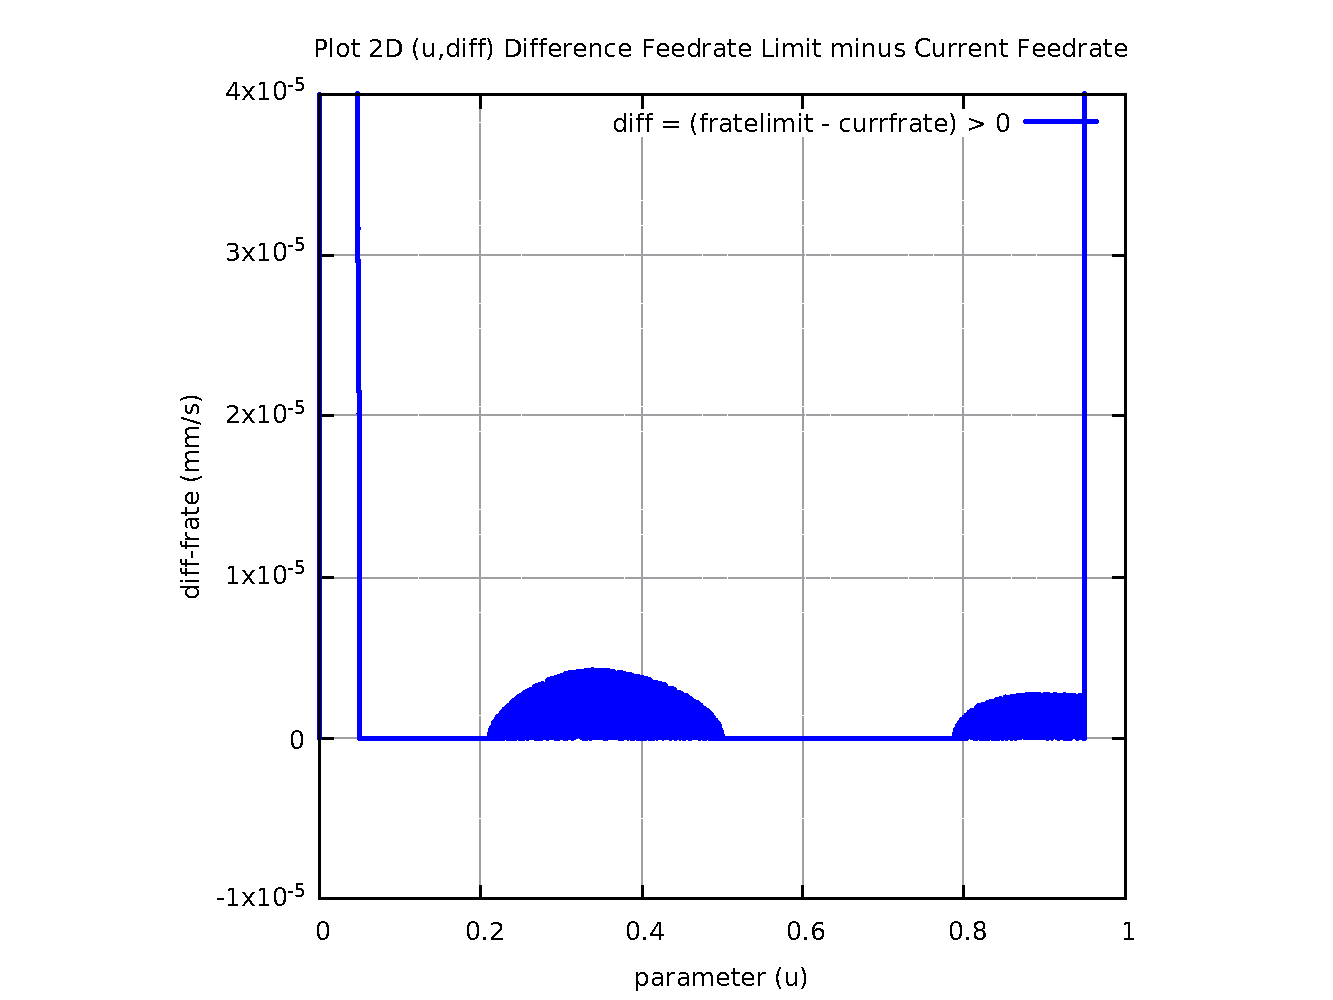
\includegraphics[width=1.00\textwidth]{Chap4/appendix/app-Circle/plots/12-img-Circle-FeedRateLimit-minus-CurrFeedRate.pdf}
\end{figure}

%% ==================================================
\clearpage
\pagebreak

\begin{figure}
	\caption     {Circle FC20-Nominal X and Y Feedrate Profiles}
	\label{13-img-Circle-FC20-Nominal-X-and-Y-Feedrate-Profiles.pdf}
	%%	\centering
	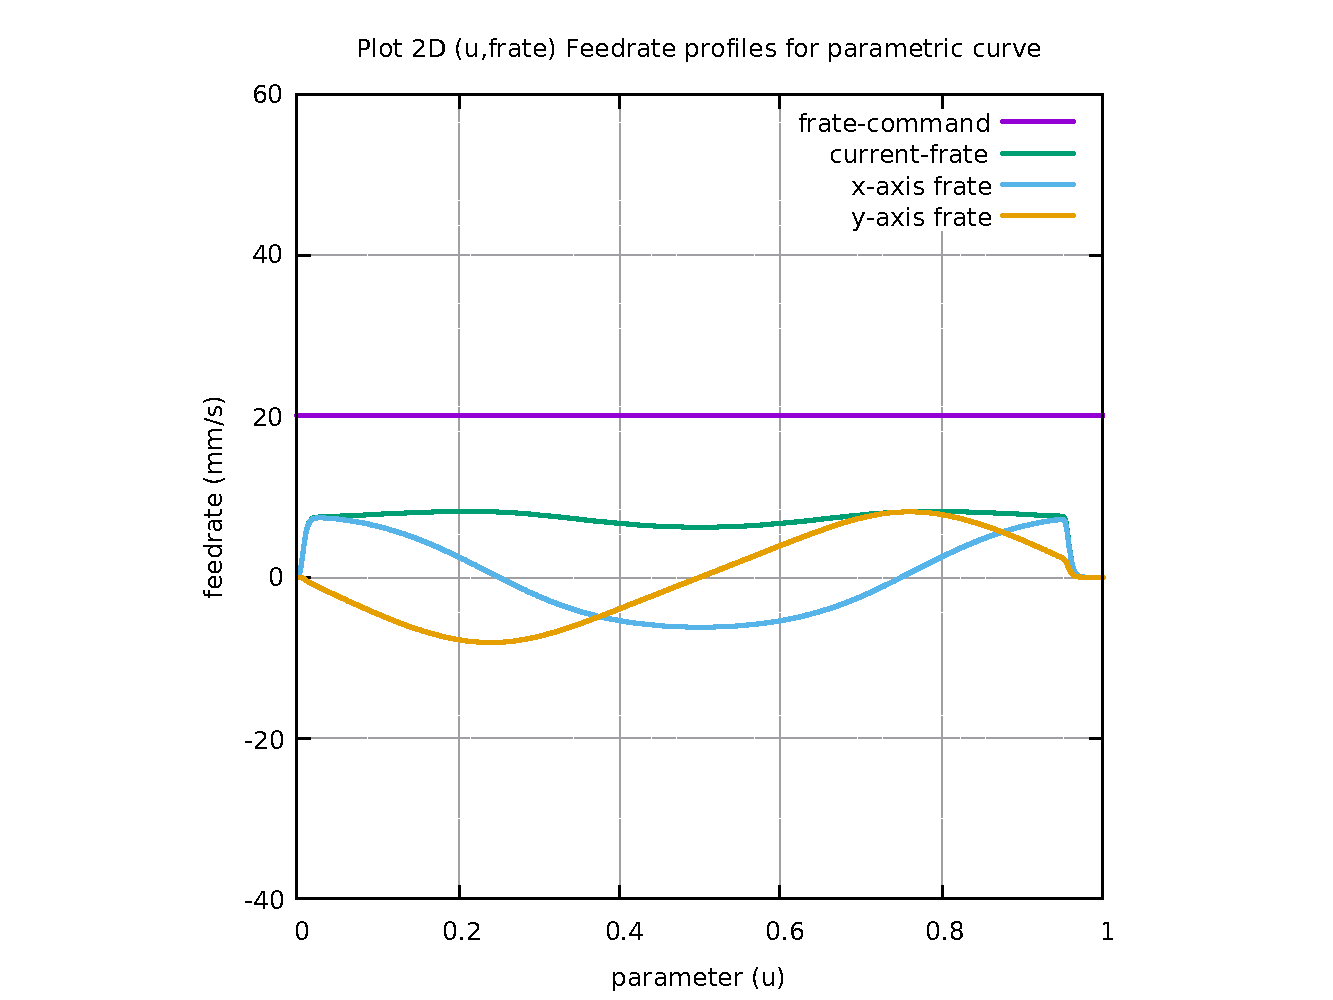
\includegraphics[width=1.00\textwidth]{Chap4/appendix/app-Circle/plots/13-img-Circle-FC20-Nominal-X-and-Y-Feedrate-Profiles.pdf}
\end{figure}


\begin{figure}
	\caption     {Circle FC20 Nominal Tangential Acceleration}
	\label{14-img-Circle-FC20-Nominal-Tangential-Acceleration.pdf}
	%%	\centering
	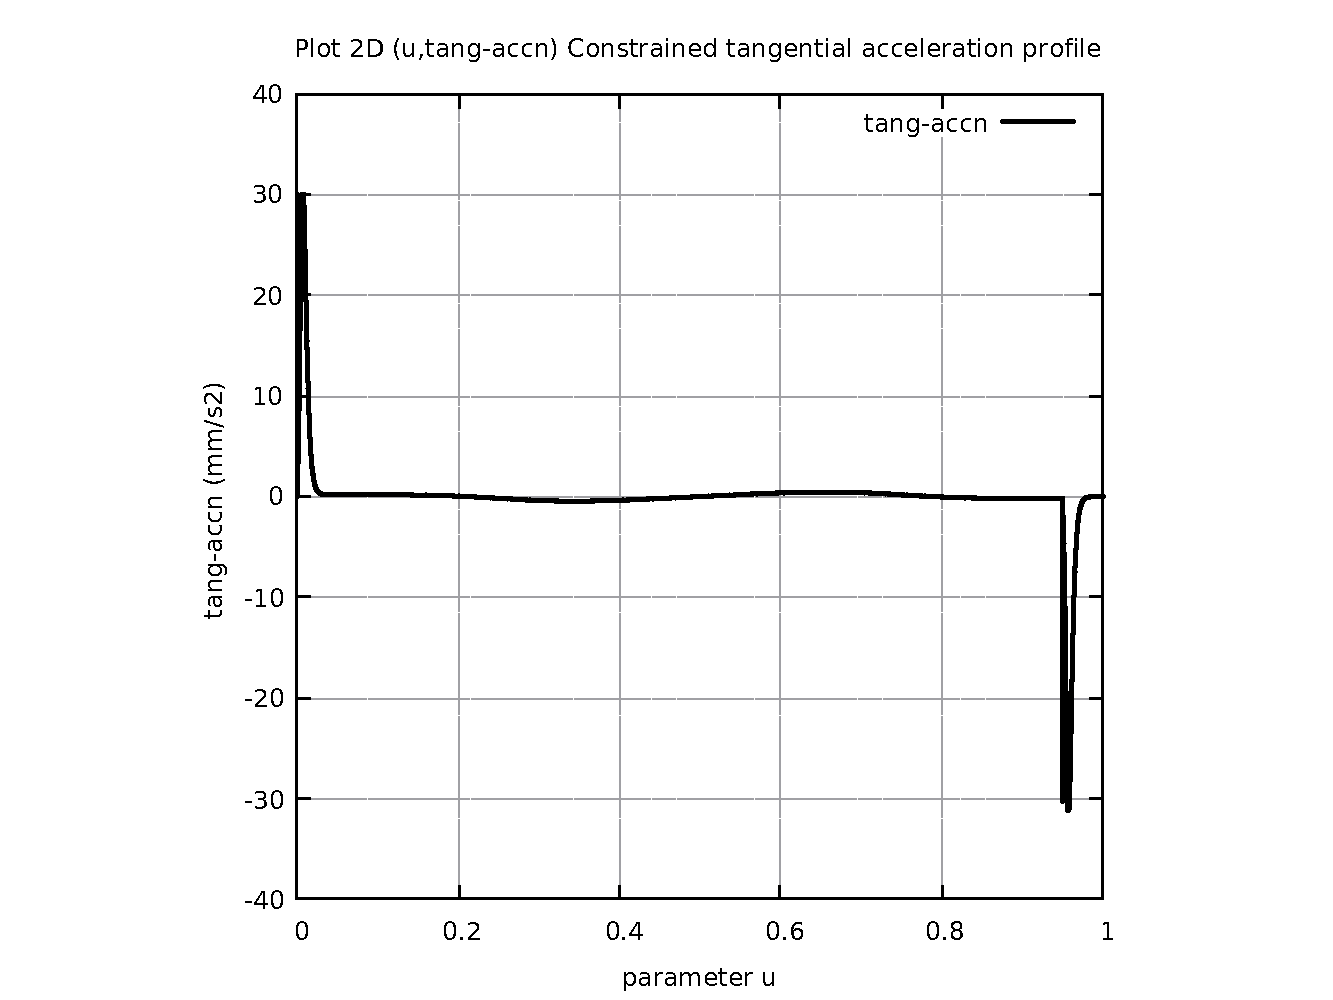
\includegraphics[width=1.00\textwidth]{Chap4/appendix/app-Circle/plots/14-img-Circle-FC20-Nominal-Tangential-Acceleration.pdf}
\end{figure}

%% ==================================================
\clearpage
\pagebreak

\begin{figure}
	\caption     {Circle FC20 Nominal Rising S-Curve Profile}
	\label{15-img-Circle-FC20-Nominal-Rising-S-Curve-Profile.pdf}
	%%	\centering
	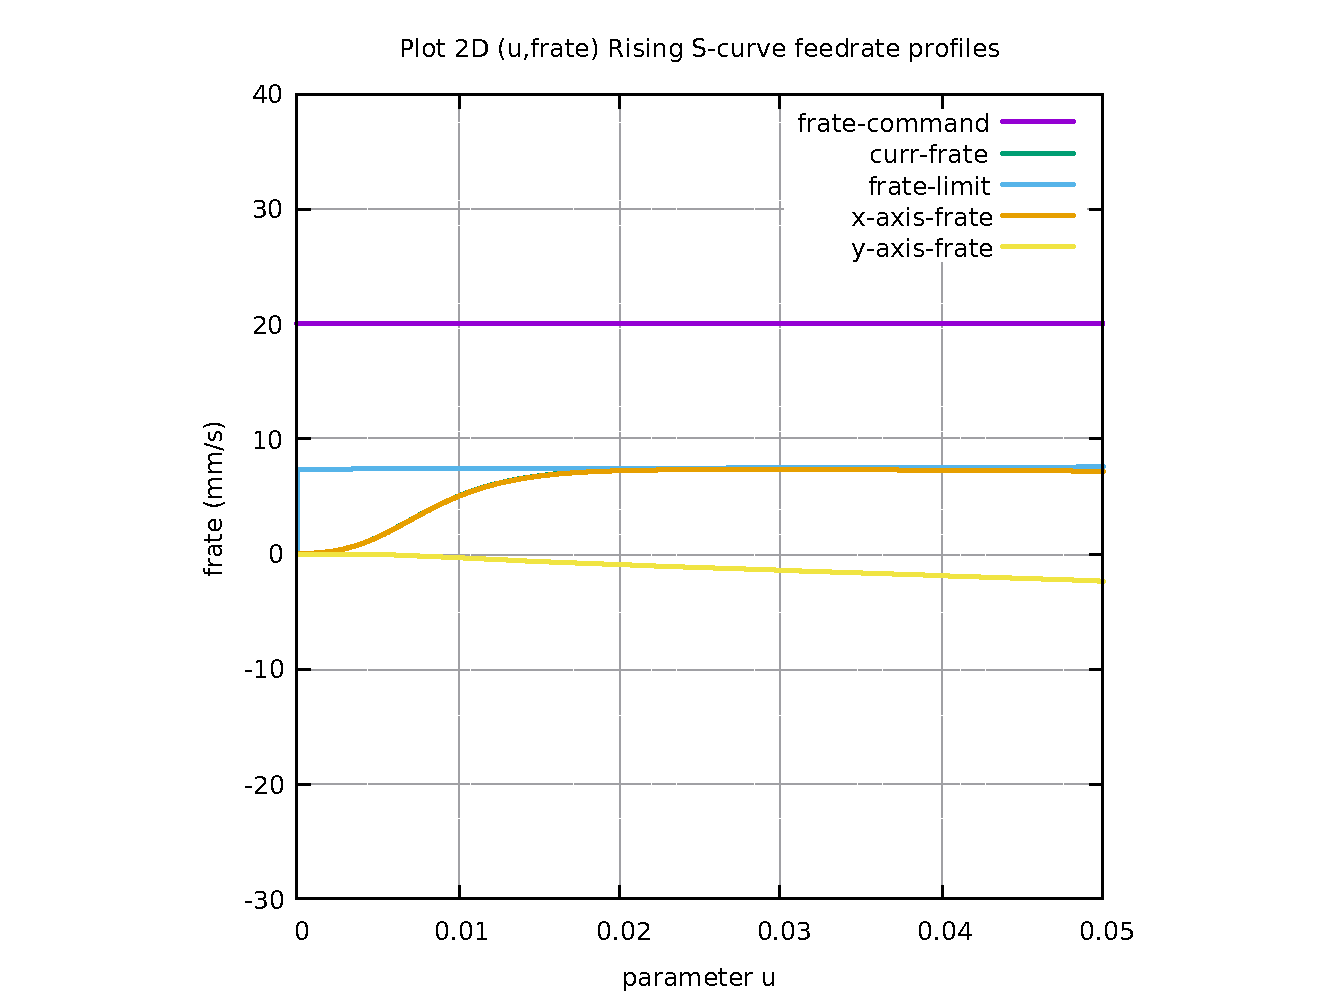
\includegraphics[width=1.00\textwidth]{Chap4/appendix/app-Circle/plots/15-img-Circle-FC20-Nominal-Rising-S-Curve-Profile.pdf}
\end{figure}


\begin{figure}
	\caption     {Circle FC20 Nominal Falling S-Curve Profile}
	\label{16-img-Circle-FC20-Nominal-Falling-S-Curve-Profile.pdf}
	%%	\centering
	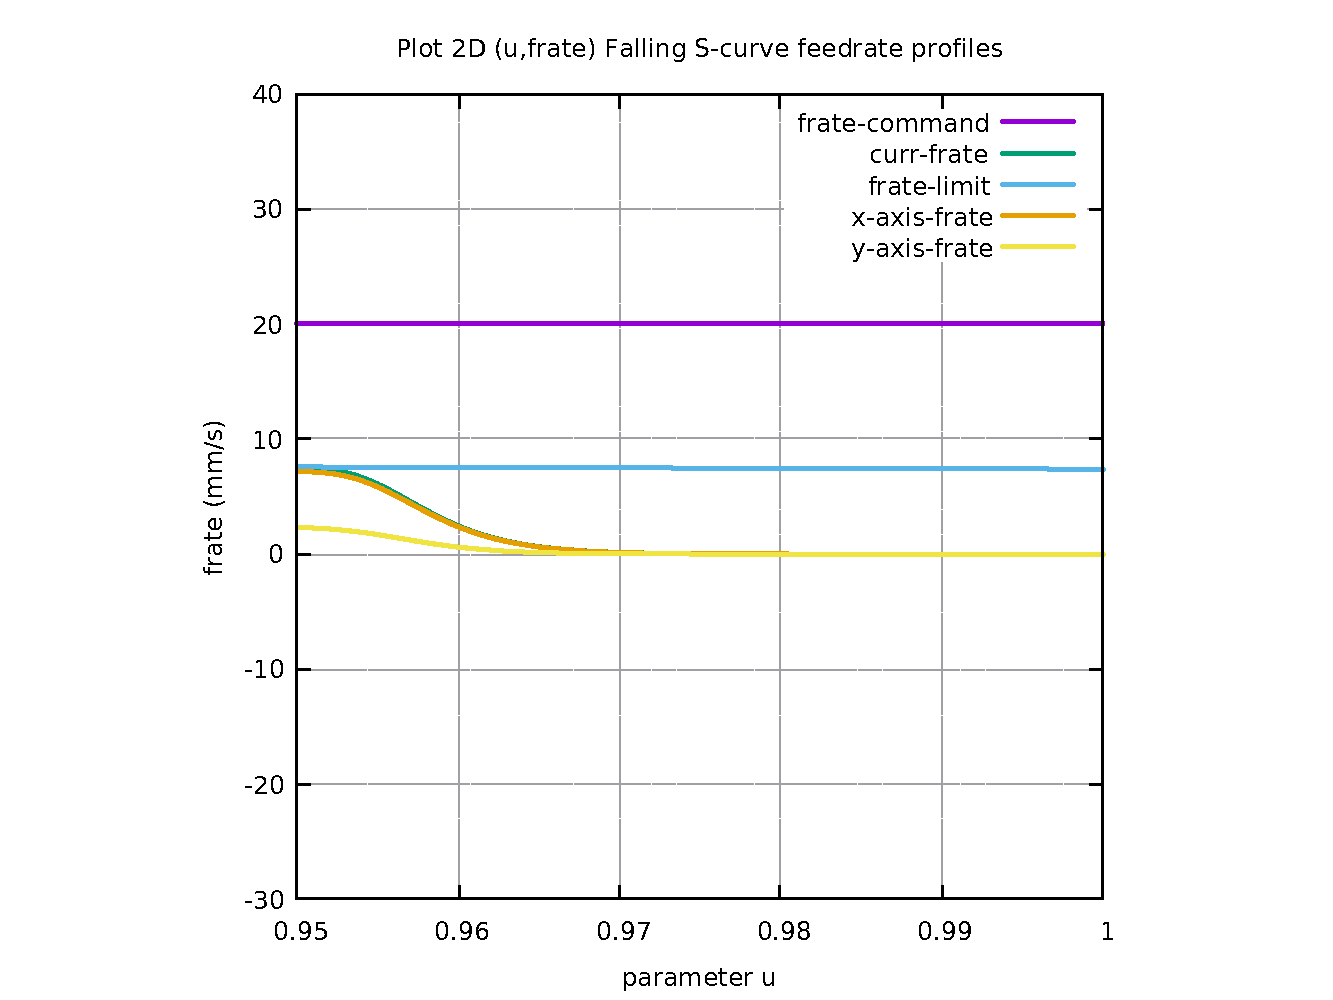
\includegraphics[width=1.00\textwidth]{Chap4/appendix/app-Circle/plots/16-img-Circle-FC20-Nominal-Falling-S-Curve-Profile.pdf}
\end{figure}

%% ==================================================
\clearpage
\pagebreak

\begin{figure}
	\caption     {Circle FC10 Colored Feedrate Profile data ngcode}
	\label{17-img-Circle-FC10-Colored-Feedrate-Profile-data_ngcode.png}
	%%	\centering
	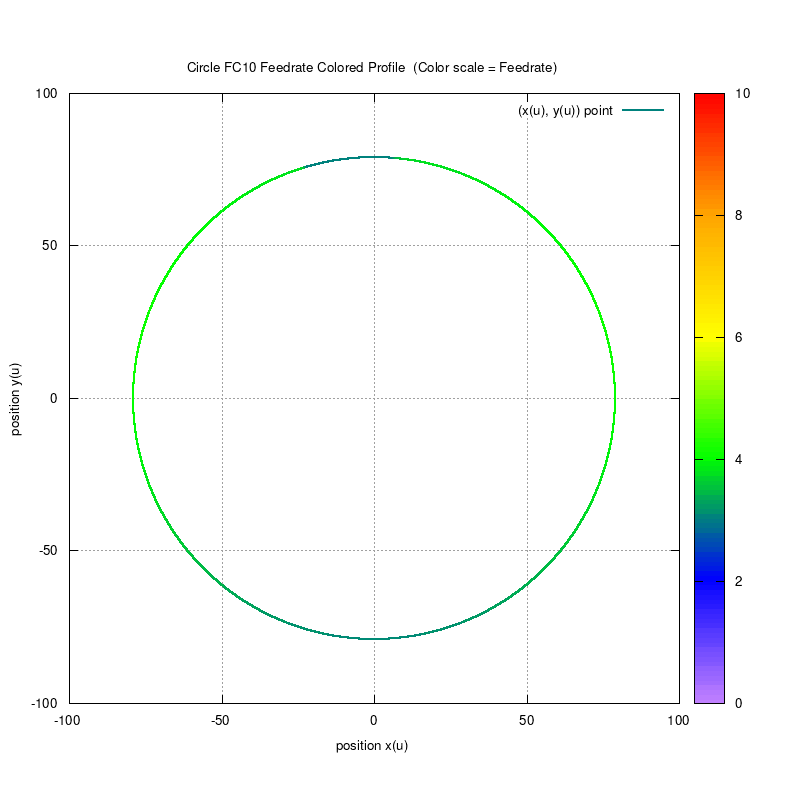
\includegraphics[width=0.75\textwidth]{Chap4/appendix/app-Circle/plots/17-img-Circle-FC10-Colored-Feedrate-Profile-data_ngcode.png}
\end{figure}


\begin{figure}
	\caption     {Circle FC20 Colored Feedrate Profile data ngcode}
	\label{18-img-Circle-FC20-Colored-Feedrate-Profile-data_ngcode.png}
	%%	\centering
	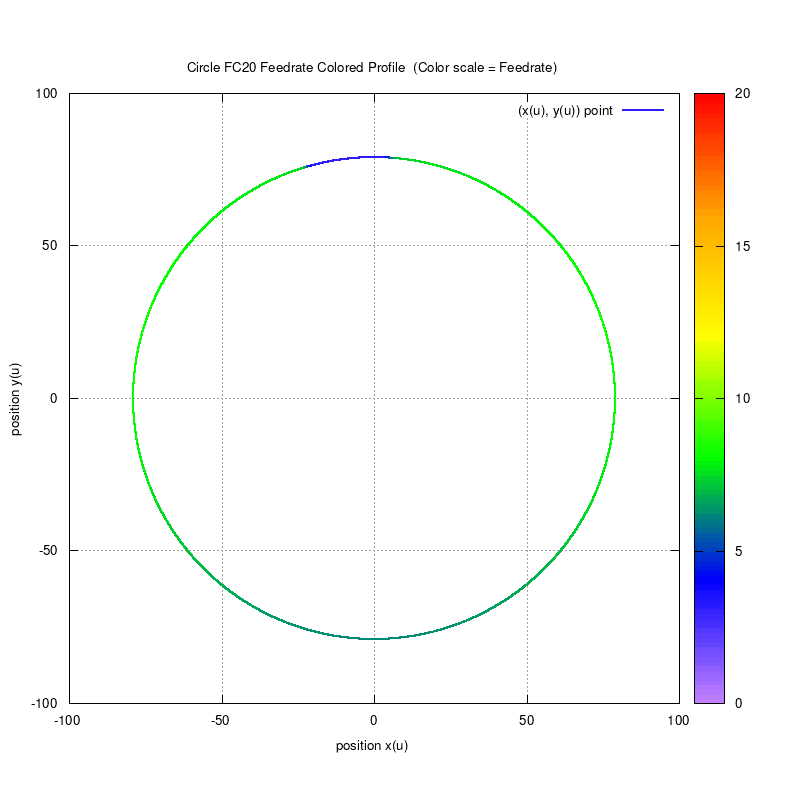
\includegraphics[width=0.75\textwidth]{Chap4/appendix/app-Circle/plots/18-img-Circle-FC20-Colored-Feedrate-Profile-data_ngcode.png}
\end{figure}

%% ==================================================
\clearpage
\pagebreak

\begin{figure}
	\caption     {Circle FC30 Colored Feedrate Profile data ngcode}
	\label{19-img-Circle-FC30-Colored-Feedrate-Profile-data_ngcode.png}
	%%	\centering
	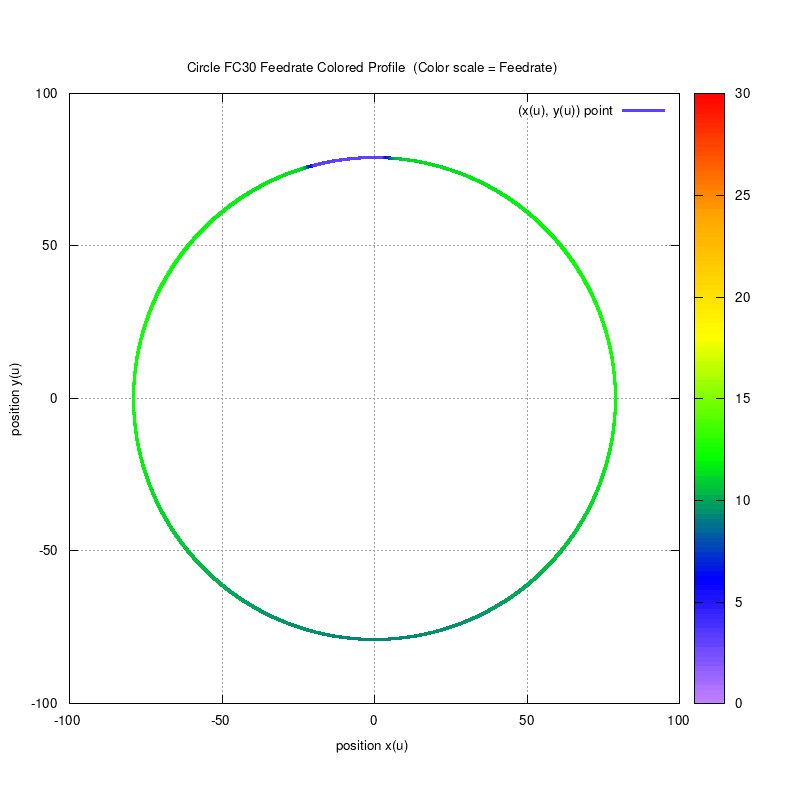
\includegraphics[width=0.75\textwidth]{Chap4/appendix/app-Circle/plots/19-img-Circle-FC30-Colored-Feedrate-Profile-data_ngcode.png}
\end{figure}


\begin{figure}
	\caption     {Circle FC40 Colored Feedrate Profile data ngcode}
	\label{20-img-Circle-FC40-Colored-Feedrate-Profile-data_ngcode.png}
	%%	\centering
	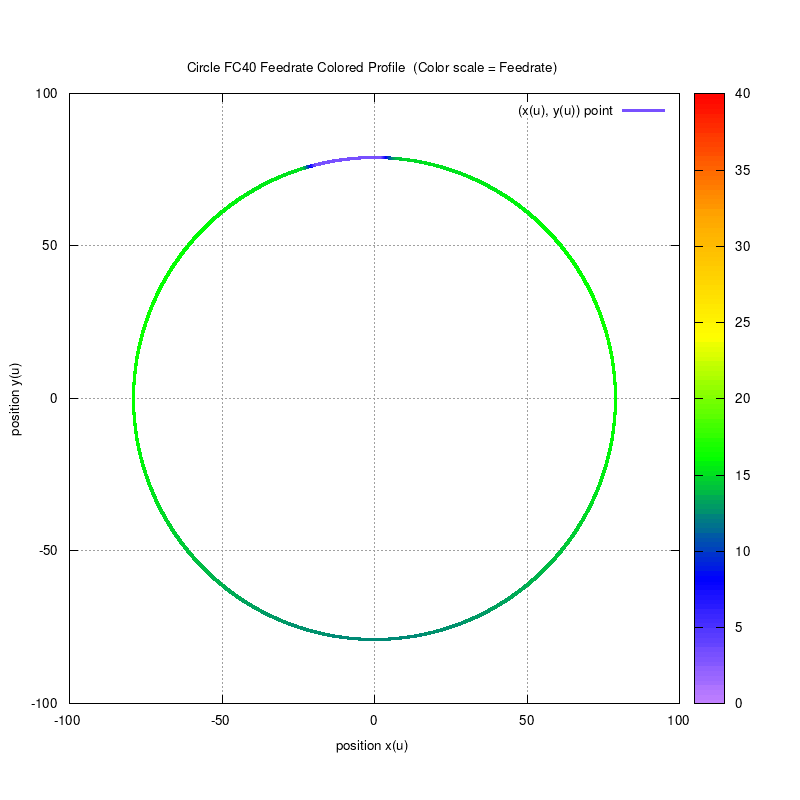
\includegraphics[width=0.75\textwidth]{Chap4/appendix/app-Circle/plots/20-img-Circle-FC40-Colored-Feedrate-Profile-data_ngcode.png}
\end{figure}

%% ==================================================
\clearpage
\pagebreak

\begin{figure}
	\caption     {Circle FC10 Tangential Acceleration}
	\label{21-img-Circle-FC10-Tangential-Acceleration.pdf}
	%%	\centering
	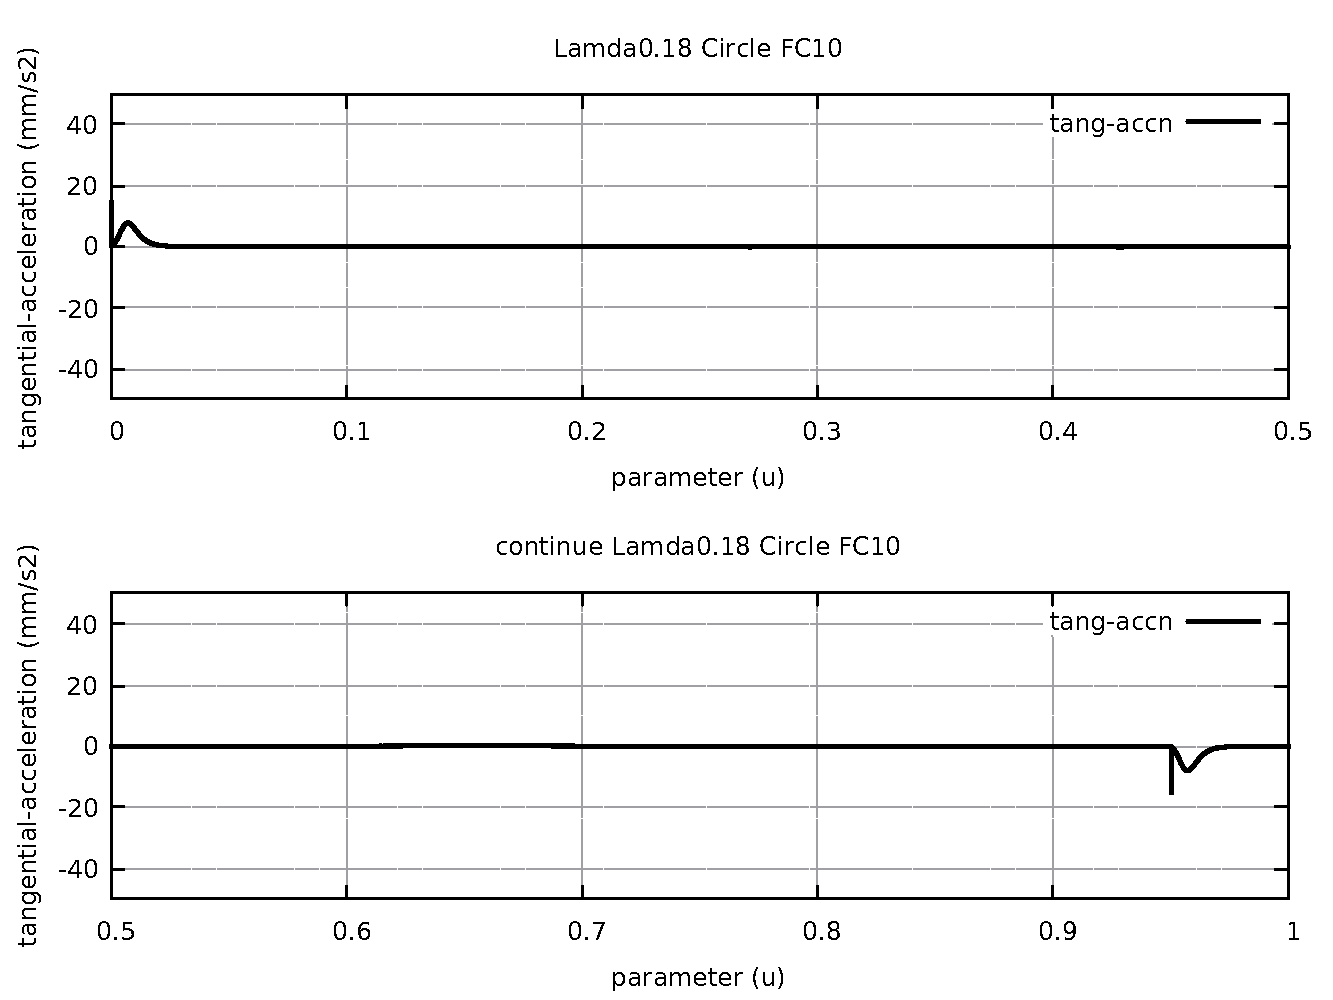
\includegraphics[width=1.00\textwidth]{Chap4/appendix/app-Circle/plots/21-img-Circle-FC10-Tangential-Acceleration.pdf}
\end{figure}


\begin{figure}
	\caption     {Circle FC20 Tangential Acceleration}
	\label{22-img-Circle-FC20-Tangential-Acceleration.pdf}
	%%	\centering
	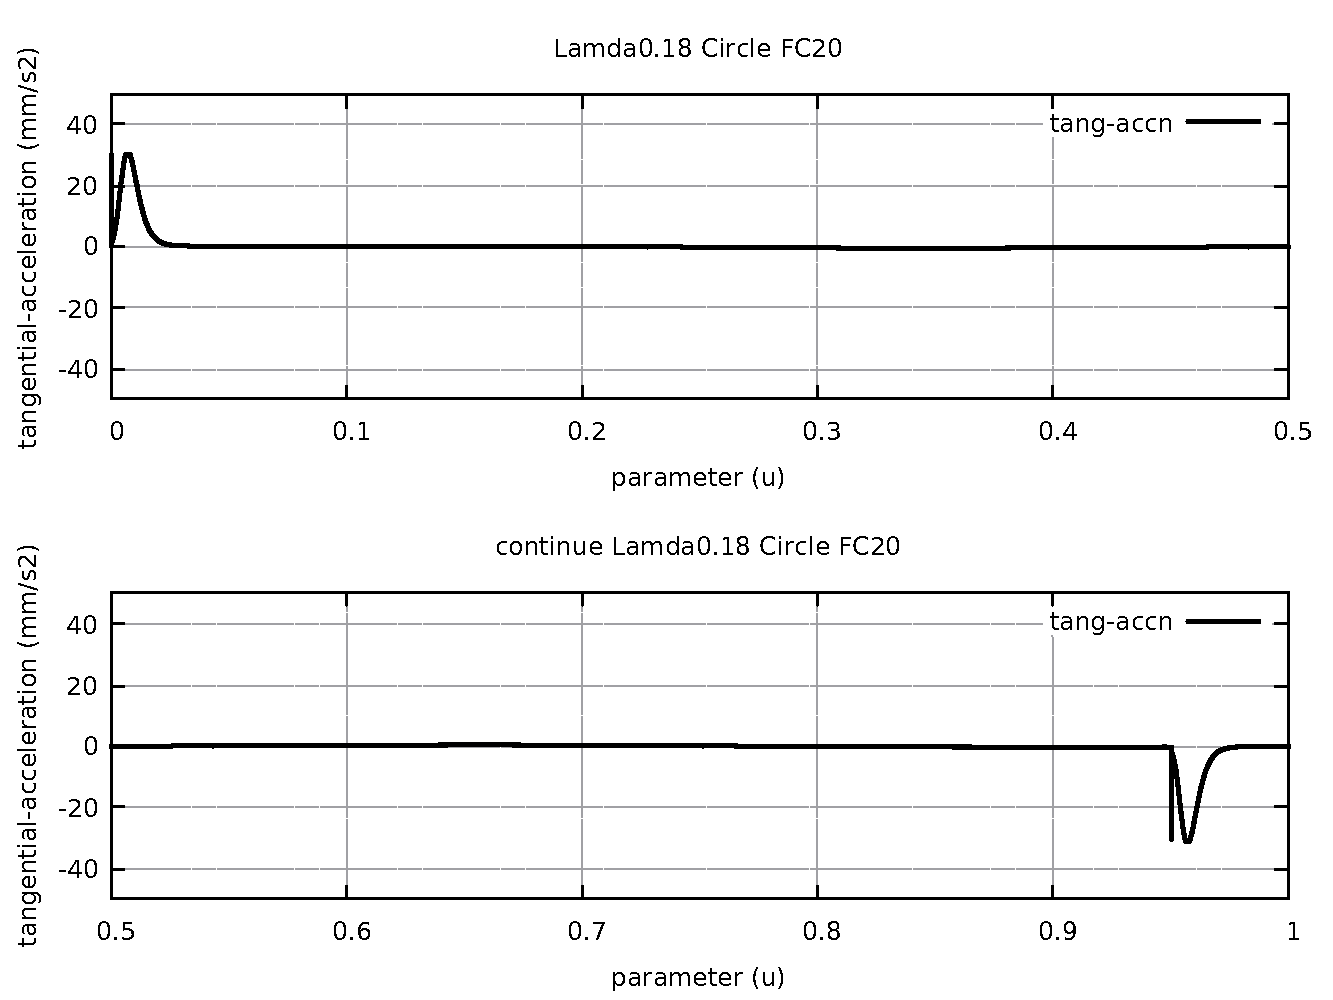
\includegraphics[width=1.00\textwidth]{Chap4/appendix/app-Circle/plots/22-img-Circle-FC20-Tangential-Acceleration.pdf}
\end{figure}

%% ==================================================
\clearpage
\pagebreak

\begin{figure}
	\caption     {Circle FC30 Tangential Acceleration}
	\label{23-img-Circle-FC30-Tangential-Acceleration.pdf}
	%%	\centering
	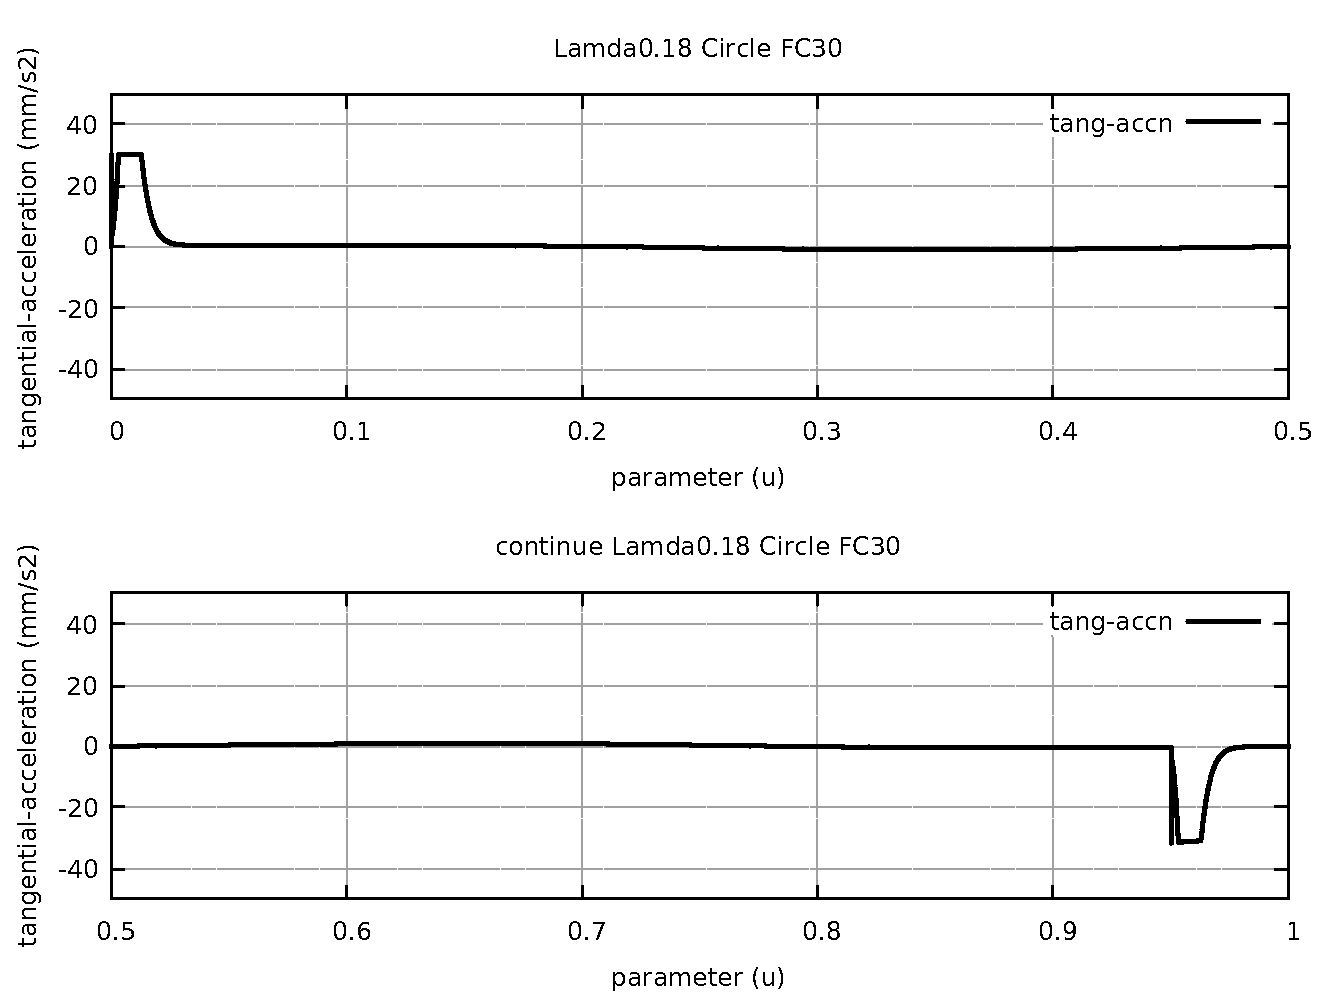
\includegraphics[width=1.00\textwidth]{Chap4/appendix/app-Circle/plots/23-img-Circle-FC30-Tangential-Acceleration.pdf}
\end{figure}


\begin{figure}
	\caption     {Circle FC40 Tangential Acceleration}
	\label{24-img-Circle-FC40-Tangential-Acceleration.pdf}
	%%	\centering
	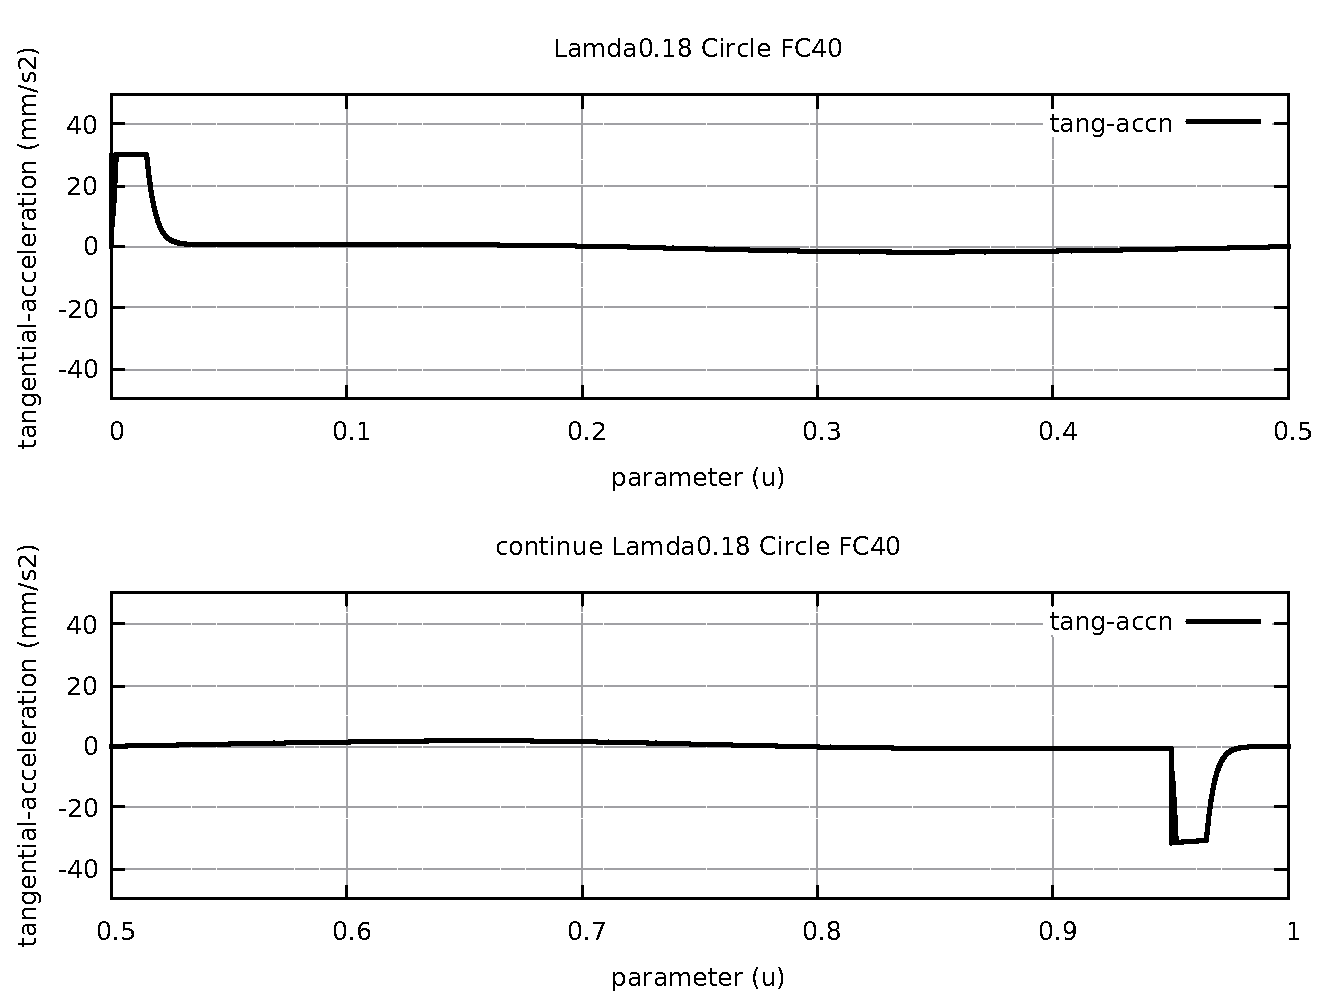
\includegraphics[width=1.00\textwidth]{Chap4/appendix/app-Circle/plots/24-img-Circle-FC40-Tangential-Acceleration.pdf}
\end{figure}

%% ==================================================
\clearpage
\pagebreak

\begin{figure}
	\caption     {Circle FC20 Nominal Separation NAL and NCL}
	\label{25-img-Circle-FC20-Nominal-Separation-NAL-and-NCL.pdf}
	%%	\centering
	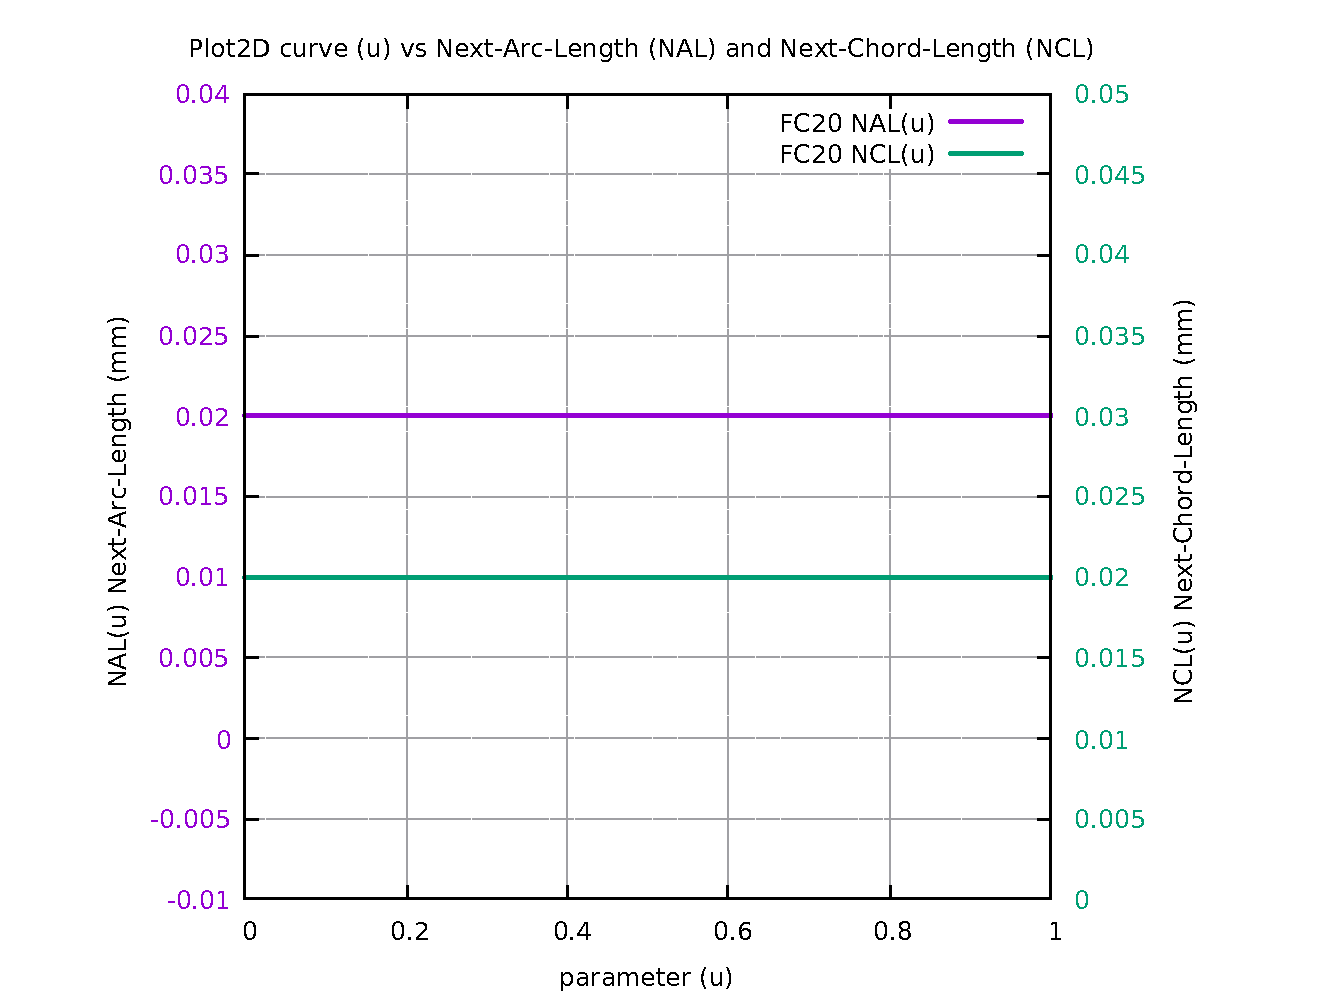
\includegraphics[width=1.00\textwidth]{Chap4/appendix/app-Circle/plots/25-img-Circle-FC20-Nominal-Separation-NAL-and-NCL.pdf}
\end{figure}


\begin{figure}
	\caption     {Circle Difference SAL minus SCL for FC10 FC20 FC30 FC40}
	\label{26-img-Circle-Difference-SAL-minus-SCL-for-FC10-FC20-FC30-FC40.pdf}
	%%	\centering
	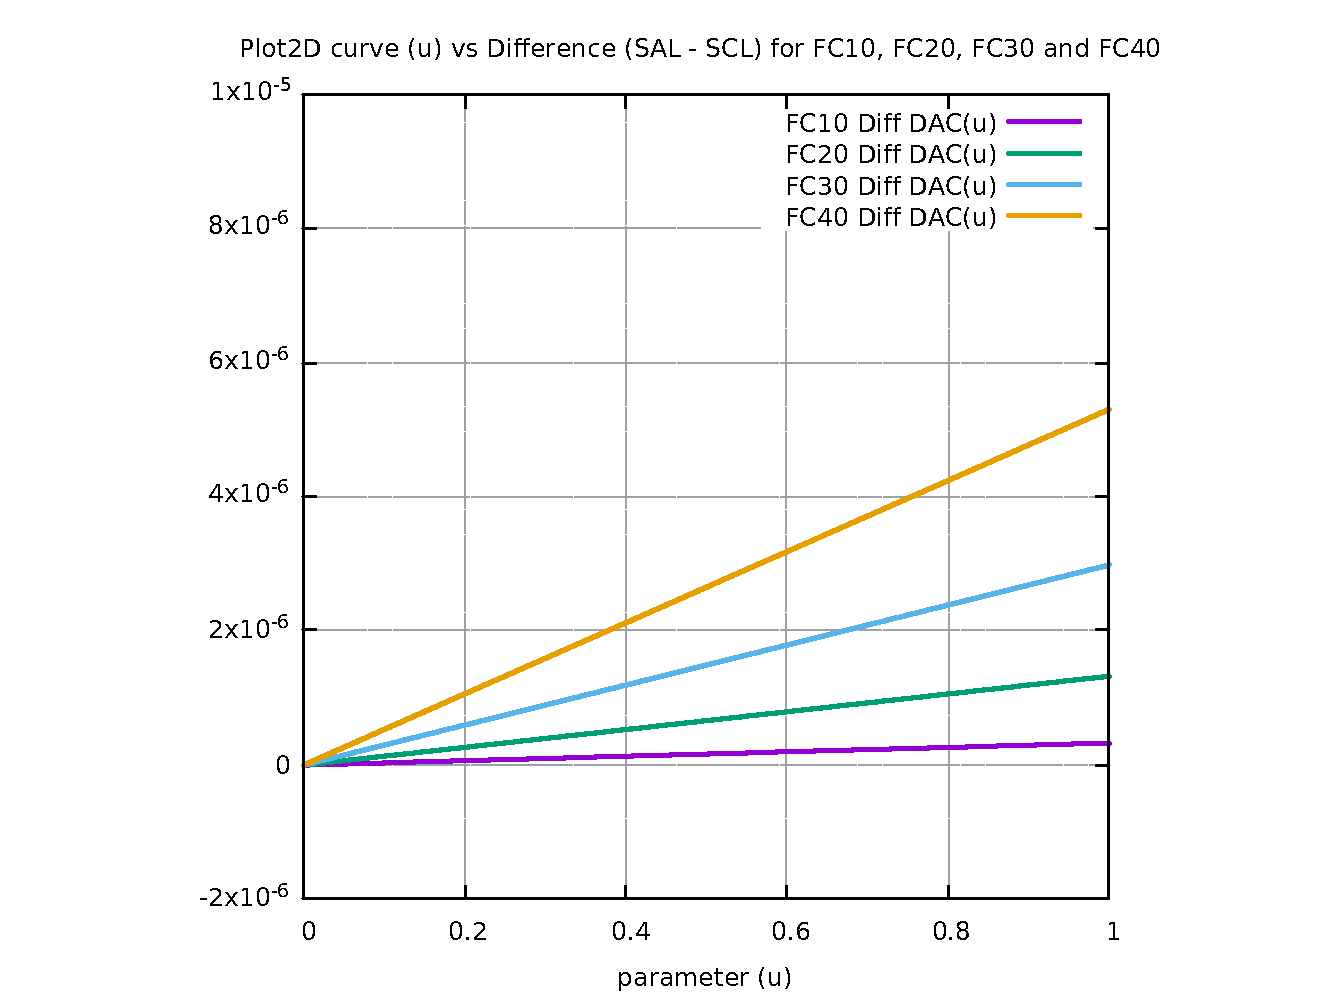
\includegraphics[width=1.00\textwidth]{Chap4/appendix/app-Circle/plots/26-img-Circle-Difference-SAL-minus-SCL-for-FC10-FC20-FC30-FC40.pdf}
\end{figure}


%% ==================================================
\clearpage
\pagebreak

\begin{figure}
	\caption     {Circle FC10 FrateCmd CurrFrate X-Frate Y-Frate}
	\label{27-img-Circle-FC10-FrateCmd-CurrFrate-X-Frate-Y-Frate.pdf}
	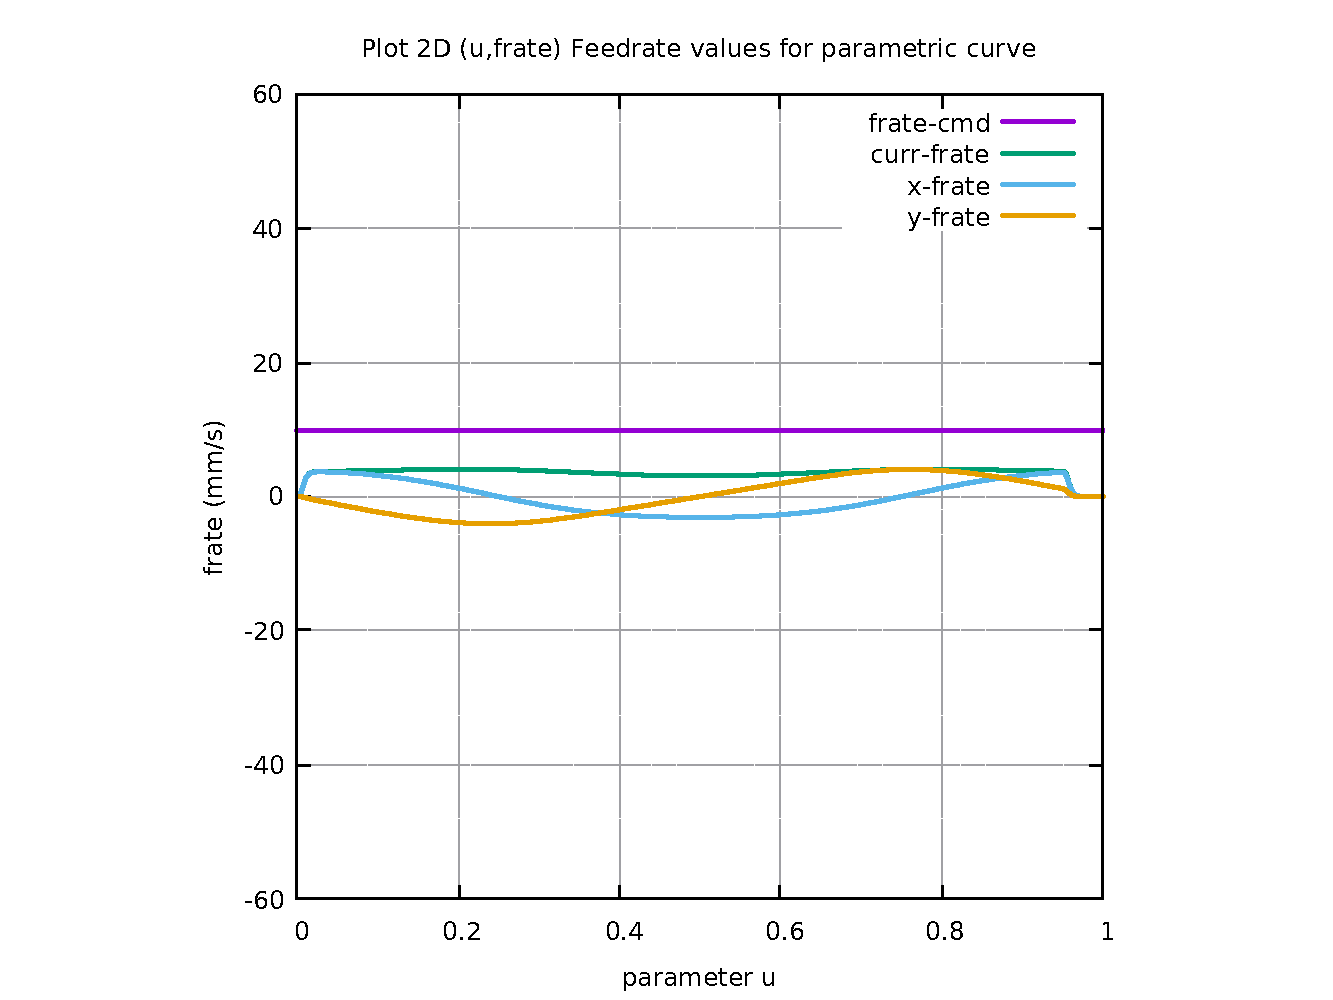
\includegraphics[width=1.00\textwidth]{Chap4/appendix/app-Circle/plots/27-img-Circle-FC10-FrateCmd-CurrFrate-X-Frate-Y-Frate.pdf}
\end{figure}


\begin{figure}
	\caption     {Circle FC20 FrateCmd CurrFrate X-Frate Y-Frate}
	\label{28-img-Circle-FC20-FrateCmd-CurrFrate-X-Frate-Y-Frate.pdf}
	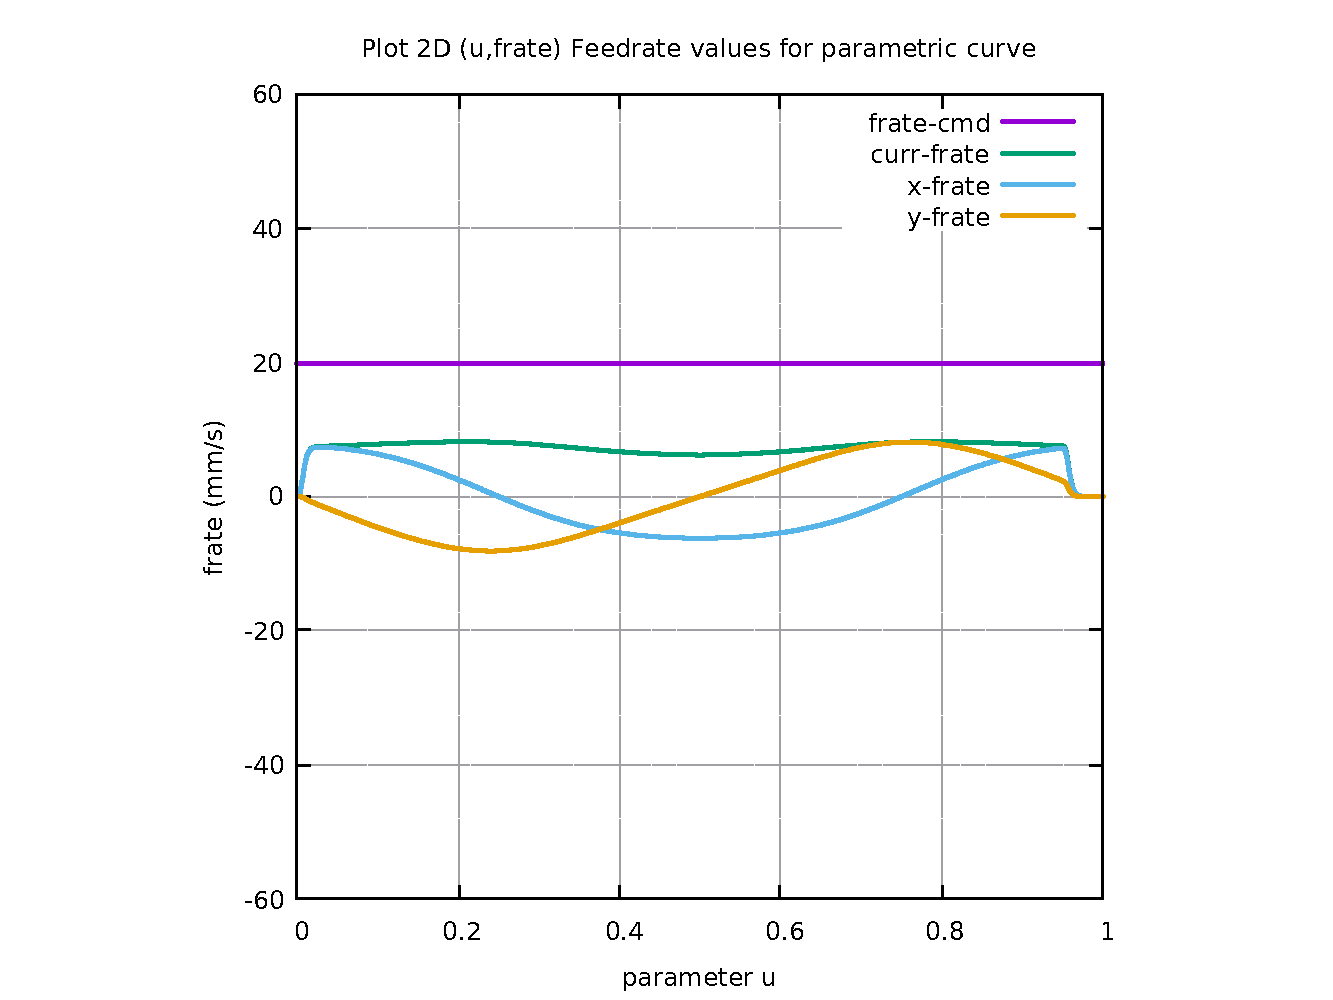
\includegraphics[width=1.00\textwidth]{Chap4/appendix/app-Circle/plots/28-img-Circle-FC20-FrateCmd-CurrFrate-X-Frate-Y-Frate.pdf}
\end{figure}


%% ==================================================
\clearpage
\pagebreak

\begin{figure}
	\caption     {Circle FC30 FrateCmd CurrFrate X-Frate Y-Frate}
	\label{29-img-Circle-FC30-FrateCmd-CurrFrate-X-Frate-Y-Frate.pdf}
	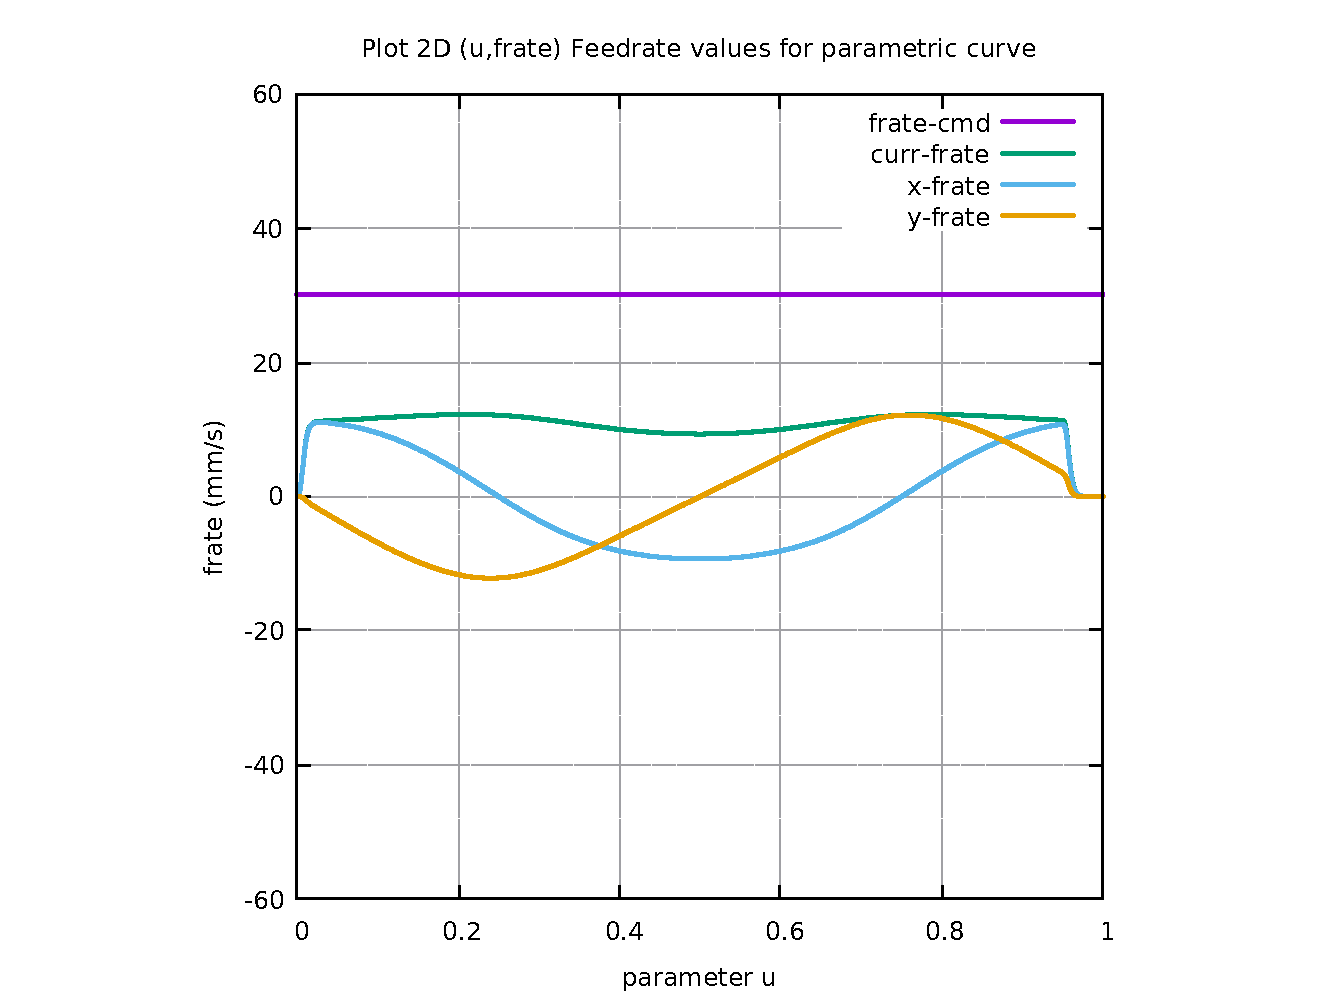
\includegraphics[width=1.00\textwidth]{Chap4/appendix/app-Circle/plots/29-img-Circle-FC30-FrateCmd-CurrFrate-X-Frate-Y-Frate.pdf}
\end{figure}


\begin{figure}
	\caption     {Circle FC40 FrateCmd CurrFrate X-Frate Y-Frate}
	\label{30-img-Circle-FC40-FrateCmd-CurrFrate-X-Frate-Y-Frate.pdf}
	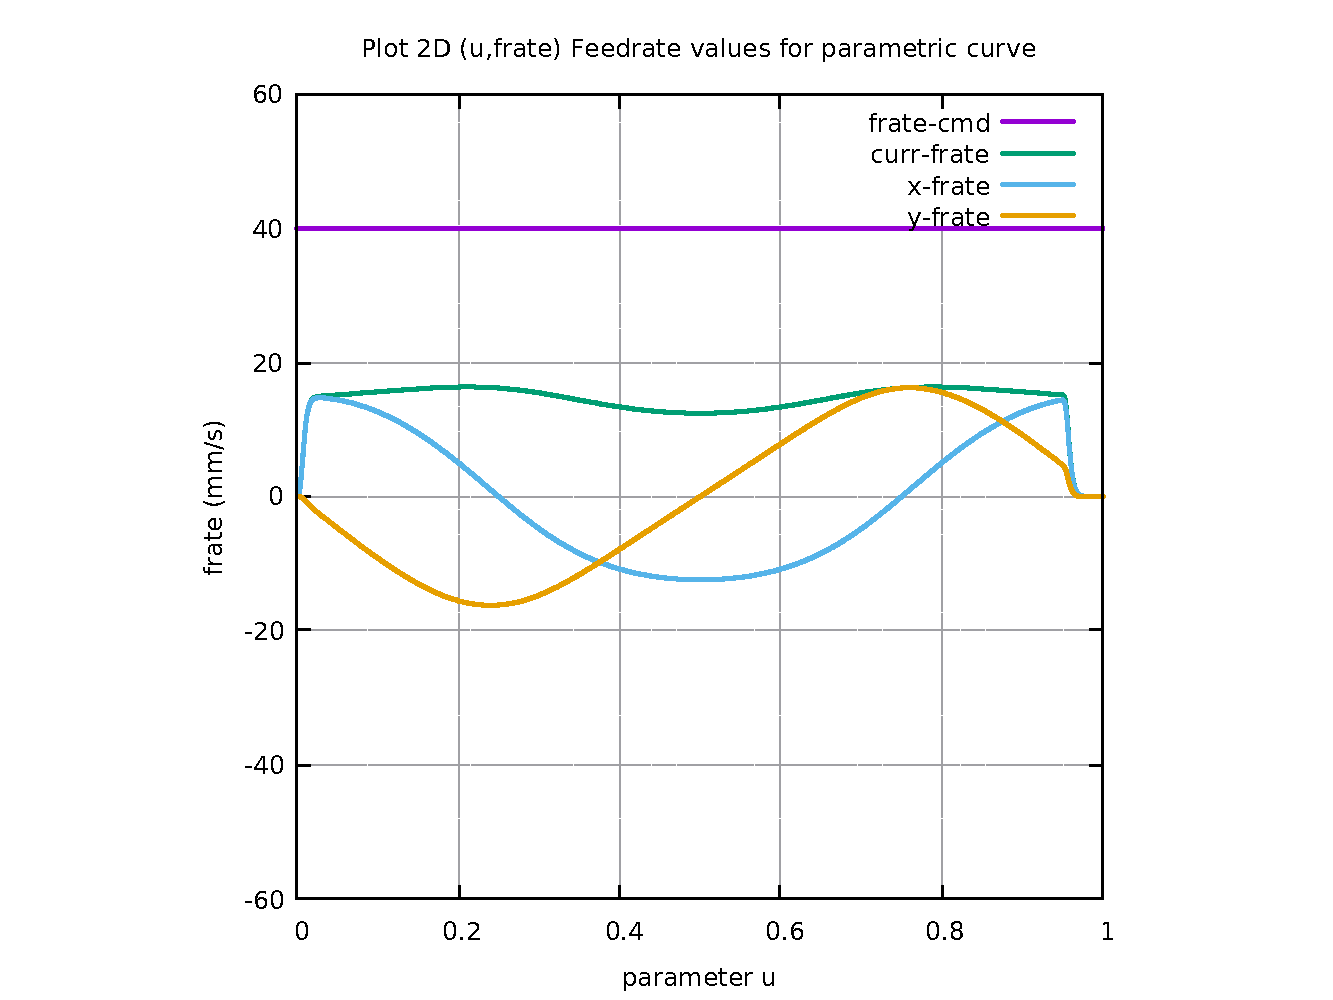
\includegraphics[width=1.00\textwidth]{Chap4/appendix/app-Circle/plots/30-img-Circle-FC40-FrateCmd-CurrFrate-X-Frate-Y-Frate.pdf}
\end{figure}


%% ==================================================
\clearpage
\pagebreak

\begin{figure}
	\caption     {Circle FC10 Four Components FeedrateLimit}
	\label{31-img-Circle-FC10-Four-Components-FeedrateLimit.pdf}
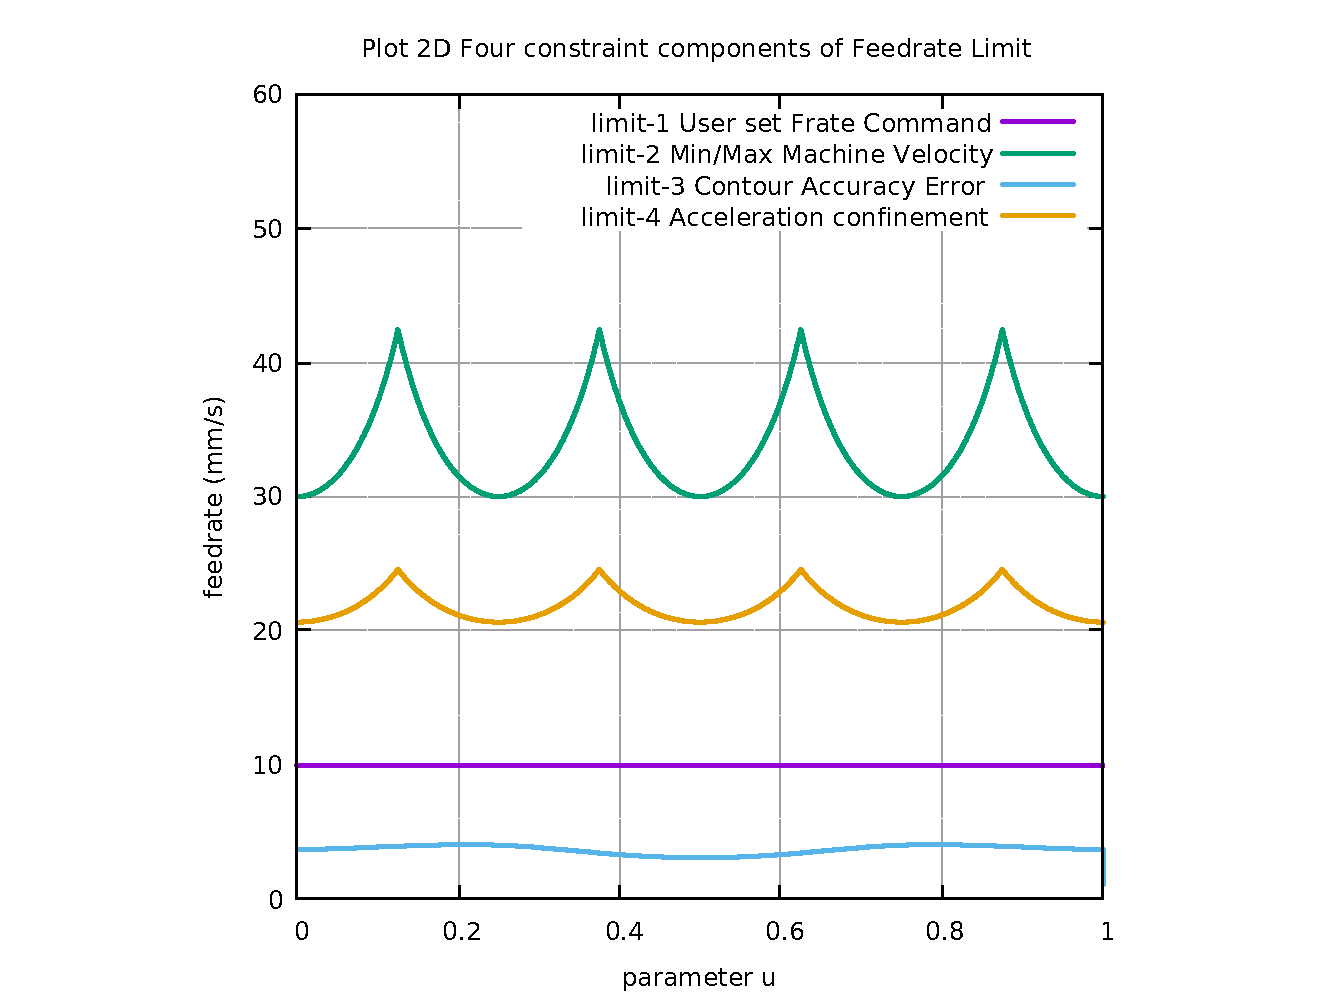
\includegraphics[width=1.00\textwidth]{Chap4/appendix/app-Circle/plots/31-img-Circle-FC10-Four-Components-FeedrateLimit.pdf}
\end{figure}


\begin{figure}
	\caption     {Circle FC20 Four Components FeedrateLimit}
	\label{32-img-Circle-FC20-Four-Components-FeedrateLimit.pdf}
	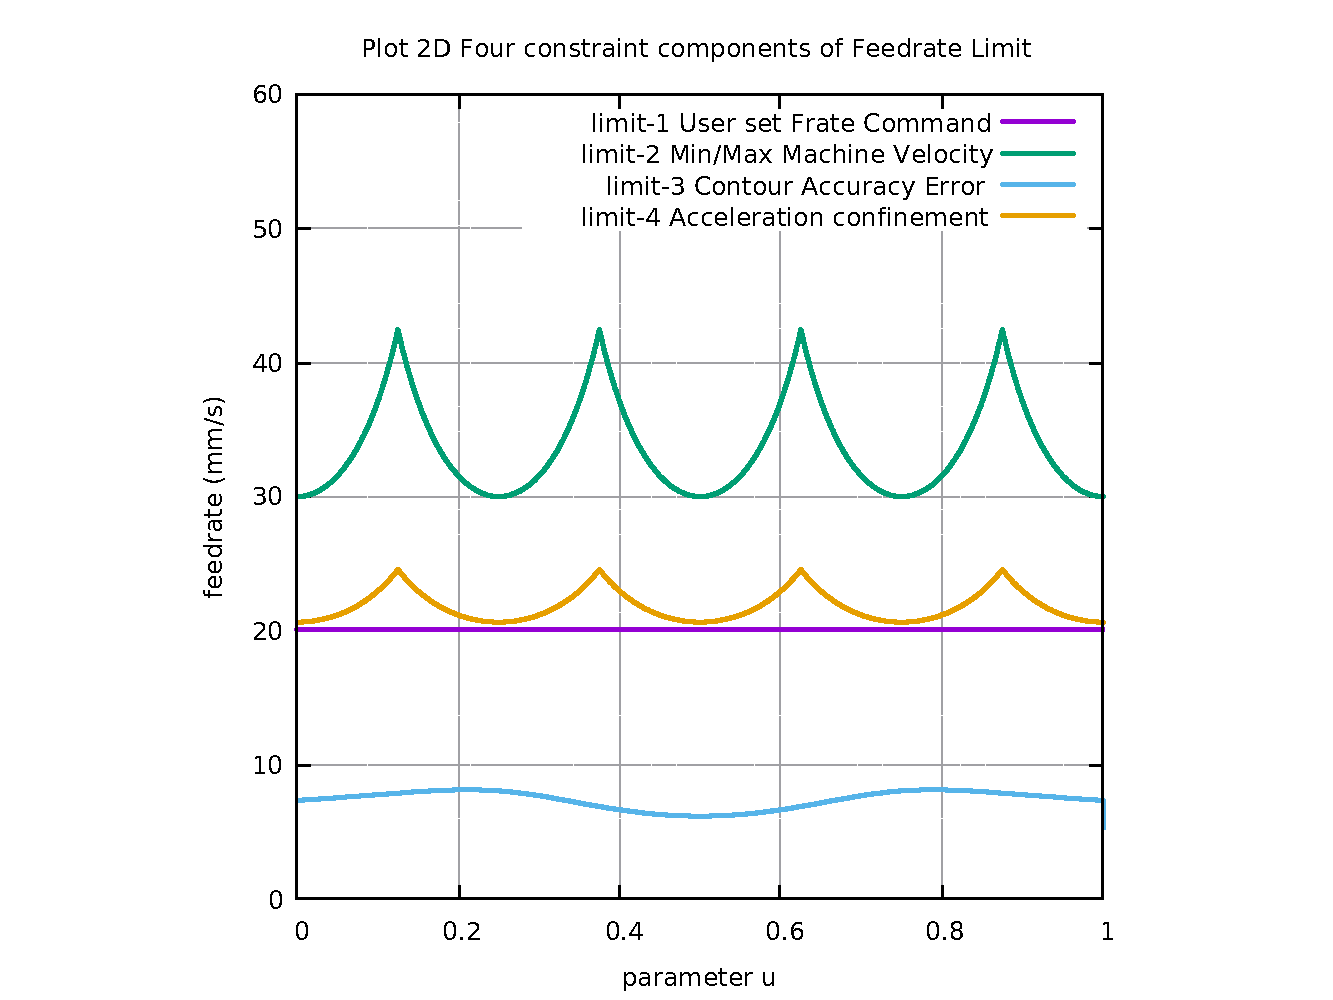
\includegraphics[width=1.00\textwidth]{Chap4/appendix/app-Circle/plots/32-img-Circle-FC20-Four-Components-FeedrateLimit.pdf}
\end{figure}


%% ==================================================
\clearpage
\pagebreak

\begin{figure}
	\caption     {Circle FC30 Four Components FeedrateLimit}
	\label{33-img-Circle-FC30-Four-Components-FeedrateLimit.pdf}
	\includegraphics[width=1.00\textwidth]{Chap4/appendix/app-Circle/plots/33-img-Circle-FC30-Four-Components-FeedrateLimit.pdf}
\end{figure}


\begin{figure}
	\caption     {Circle FC40 Four Components FeedrateLimit}
	\label{34-img-Circle-FC40-Four-Components-FeedrateLimit.pdf}
	\includegraphics[width=1.00\textwidth]{Chap4/appendix/app-Circle/plots/34-img-Circle-FC40-Four-Components-FeedrateLimit.pdf}
\end{figure}

%% =======================================
\clearpage
\pagebreak

\begin{figure}
	\centering
	\caption     {Circle Histogram Points FC10 FC20 FC30 FC40}
	\label{35-img-Circle-Histogram-Points-FC10-FC20-FC30-FC40.pdf}
	\includegraphics[width=1.00\textwidth]{Chap4/appendix/app-Circle/plots/35-img-Circle-Histogram-Points-FC10-FC20-FC30-FC40.pdf} 
\end{figure}


\begin{table}[ht]
%% \begin{center}
\caption    {Circle Table distribution of interpolated points}
\label  {tab-Circle Table distribution of interpolated points}
	
%% IMPORTANT TO SCALEBOX BELOW
\scalebox{0.80}{
		
%% START COPY AND PASTE BELOW HERE
%% FROM \begin{tabular} UNTIL \end{tabular)
%% Note: adjust last p{} to get line width correct
		
\begin{tabular}{ p{4.5cm} p{1.5cm} p{1.5cm} p{1.5cm} p{7.50cm} }
\hline
&		&		&		&		\\
BINS	&	FC10	&	FC20	&	FC30	&	FC40	\\
&		&		&		&		\\
0.0 - 0.1	&	4964	&	2482	&	1654	&	1241	\\
0.1 - 0.2	&	4964	&	2482	&	1655	&	1241	\\
0.2 - 0.3	&	4964	&	2482	&	1655	&	1241	\\
0.3 - 0.4	&	4964	&	2482	&	1655	&	1241	\\
0.4 - 0.5	&	4964	&	2482	&	1655	&	1242	\\
0.5 - 0.6	&	4964	&	2483	&	1655	&	1241	\\
0.6 - 0.7	&	4964	&	2482	&	1655	&	1241	\\
0.7 - 0.8	&	4964	&	2482	&	1655	&	1241	\\
0.8 - 0.9	&	4964	&	2482	&	1654	&	1242	\\
0.9 - 1.0	&	4965	&	2483	&	1656	&	1242	\\
&		&		&		&		\\
Tot Counts	&	49641	&	24822	&	16549	&	12413	\\
&		&		&		&		\\
\hline	
\end{tabular}
		
%% END COPY AND PASTE ABOVE HERE
		
}   %% IMPORTANT FOR SCALEBOX CLOSING
	
\hrule
\end{table}
%% \end{landscape}

%% CIRCLE SUMMARY TABLE
%% ========================================================
\clearpage
\pagebreak
\begin{landscape}
	
\begin{table}[ht]
%% \begin{center}
\caption       {Circle Table FC10-20-30-40 Run Performance data}
\label{tab-app4-Circle-Table-FC10-20-30-40-Run-Performance-data}

%% IMPORTANT TO SCALEBOX BELOW
\scalebox{0.90}{
			
%% START COPY AND PASTE BELOW HERE
%% FROM \begin{tabular} UNTIL \end{tabular)
			
\begin{tabular}{ p{0.2cm} p{8.80cm} p{4.00cm} p{4.0cm} p{4.00cm} p{4.0cm}}
\hline
				&		&		&		&		&		\\
				1	&	Curve Type	&	CIRCLE	&	CIRCLE	&	CIRCLE	&	CIRCLE	\\
				2	&	User Feedrate Command FC(mm/s)                   	&	FC10	&	FC20	&	FC30	&	FC40	\\
				3	&	User Lamda Acceleration Safety Factor	&	0.18	&	0.18	&	0.18	&	0.18	\\
				&		&		&		&		&		\\
				4	&	Total Iterpolated Points (TIP)	&	49641	&	24822	&	16549	&	12413	\\
				5	&	Total Sum-Chord-Error (SCE) (mm)	&	1.093913738449E-03	&	2.187639876000E-03	&	3.281178287065E-03	&	4.374701201686E-03	\\
				6	&	Ratio 1 = (SCE/TIP) = Chord-Error/Point	&	2.203694074232E-08	&	8.813665347893E-08	&	1.982824683989E-07	&	3.524573962041E-07	\\
				&		&		&		&		&		\\
				7	&	Total Sum-Arc-Length (SAL) (mm)	&	4.963785816452E+02	&	4.963771594934E+02	&	4.963757335444E+02	&	4.963942987341E+02	\\
				8	&	Total Sum-Chord-Length (SCL) (mm)	&	4.963785813150E+02	&	4.963771581682E+02	&	4.963757305630E+02	&	4.963942934342E+02	\\
				9	&	Difference = (SAL – SCL) (mm)	&	3.302195636934E-07	&	1.325165840171E-06	&	2.981455850204E-06	&	5.299917688717E-06	\\
				10	&	Percentage Difference = (SAL – SCL)/SAL	&	6.652574786747E-08	&	2.669675295946E-07	&	6.006449648363E-07	&	1.067683029848E-06	\\
				&		&		&		&		&		\\
				11	&	Ratio 2 = (SCE/SCL) = Chord Error/Chord-Length	&	2.203789163406E-06	&	4.407213023407E-06	&	6.610271383220E-06	&	8.812956271960E-06	\\
				&		&		&		&		&		\\
				12	&	Total Sum-Arc-Theta (SAT) (rad)	&	6.283146611127E+00	&	6.283002050952E+00	&	6.282857458743E+00	&	6.282965934945E+00	\\
				13	&	Total Sum-Arc-Area (SAA) (mm2)	&	5.235292684461E-05	&	2.093803820914E-04	&	4.710353817982E-04	&	8.373046676549E-04	\\
				&		&		&		&		&		\\
				14	&	Ratio 3 = (SAA/SCL) = Arc-Area/Chord-Length	&	2.203789163406E-06	&	4.407213023407E-06	&	6.610271383220E-06	&	8.812956271960E-06	\\
				&		&		&		&		&		\\
				15	&	Average-Chord-Error (ACE) (mm)	&	2.203694074232E-08	&	8.813665347893E-08	&	1.982824683989E-07	&	3.524573962041E-07	\\
				16	&	Average-Arc-Length (AAL) (mm)	&	9.999568526293E-03	&	1.999827402173E-02	&	2.999611636116E-02	&	3.999309528956E-02	\\
				17	&	Average-Chord-Length (ACL) (mm)	&	9.999568519641E-03	&	1.999827396834E-02	&	2.999611618099E-02	&	3.999309486257E-02	\\
				18	&	Average-Arc-Theta (AAT) (rad)	&	1.265742669445E-04	&	2.531325108155E-04	&	3.796747316136E-04	&	5.062009293381E-04	\\
				19	&	Average-Arc-Area (AAA) (mm2)	&	1.054652031519E-09	&	8.435614281914E-09	&	2.846479222856E-08	&	6.745928679140E-08	\\
				&		&		&		&		&		\\
				20	&	Algorithm actual runtime on computer (ART) (s) 	&	17.277667419	&	8.160163431	&	5.399371536	&	4.053925000	\\
				&		&		&		&		&	\\	
\hline				
\end{tabular}
			
%% END COPY AND PASTE		
}   %% IMPORTANT FOR SCALEBOX CLOSING
\end{table}
\end{landscape}

%% =====================================================
%% ==================================================

\section{\textbf{APPENDIX ELLIPSE CURVE}} \label{APPENDIX ELLIPSE CURVE}


\subsection       {Plot of Ellipse curve
	[\ref  {01-img-Plot of Ellipse curve.pdf} ] }
\label{ssec-01-img-Plot of Ellipse curve.pdf}

\subsection       {Ellipse Radius of Curvature
[\ref      {02-img-Ellipse Radius of Curvature.pdf}] }
\label{ssec-02-img-Ellipse Radius of Curvature.pdf}

\subsection       {Ellipse Validation in LinuxCNC
[\ref      {03-img-Ellipse-Validation-in-LinuxCNC.png} ] }
\label{ssec-03-img-Ellipse-Validation-in-LinuxCNC.png}

\subsection     {Ellipse Direction of Travel 3D
[\ref      {04-img-Ellipse Direction of Travel 3D.pdf} ] }
\label{ssec-04-img-Ellipse Direction of Travel 3D.pdf}

\subsection       {Ellipse First and Second Order Taylor's Approx
[\ref      {05-img-Ellipse-First-and-Second-Order-Taylors-Approx.pdf}] }
\label{ssec-05-img-Ellipse-First-and-Second-Order-Taylors-Approx.pdf}

\subsection       {Ellipse First minus Second Order Taylor's Approx
[\ref      {06-img-Ellipse-First-minus-Second-Order-Taylors-Approx.pdf}] }
\label{ssec-06-img-Ellipse-First-minus-Second-Order-Taylors-Approx.pdf}

\subsection       {Ellipse Separate First and Second Order Taylor's Approx
[\ref      {07-img-Ellipse-Separation-First-and-Second-Order-Taylors-Approx.pdf} ] }
\label{ssec-07-img-Ellipse-Separation-First-and-Second-Order-Taylors-Approx.pdf}

\subsection       {Ellipse Separation SAL and SCL
[\ref      {08-img-Ellipse-Separation-SAL-and-SCL.pdf}] }
\label{ssec-08-img-Ellipse-Separation-SAL-and-SCL.pdf}

\subsection       {Ellipse Chord-error in close view 2 scales
[\ref      {09-img-Ellipse-Chord-error-in-close-view-2-scales.pdf}] }
\label{ssec-09-img-Ellipse-Chord-error-in-close-view-2-scales.pdf}

\subsection       {Ellipse Four Components Feedrate Limit
[\ref      {10-img-Ellipse-Four-Components-Feedrate-Limit.pdf} ] }
\label{ssec-10-img-Ellipse-Four-Components-Feedrate-Limit.pdf}

\subsection    {Ellipse FrateCommand FrateLimit and Curr-Frate
[\ref      {11-img-Ellipse-FrateCommand-FrateLimit-and-Curr-Frate.pdf}] }
\label{ssec-11-img-Ellipse-FrateCommand-FrateLimit-and-Curr-Frate.pdf}

\subsection     {Ellipse FeedRateLimit minus CurrFeedRate
[\ref      {12-img-Ellipse-FeedRateLimit-minus-CurrFeedRate.pdf} ] }
\label{ssec-12-img-Ellipse-FeedRateLimit-minus-CurrFeedRate.pdf}

\subsection     {Ellipse FC20-Nominal X and Y Feedrate Profiles
[\ref      {13-img-Ellipse-FC20-Nominal-X-and-Y-Feedrate-Profiles.pdf} ] }
\label{ssec-13-img-Ellipse-FC20-Nominal-X-and-Y-Feedrate-Profiles.pdf}

\subsection     {Ellipse FC20 Nominal Tangential Acceleration
[\ref      {14-img-Ellipse-FC20-Nominal-Tangential-Acceleration.pdf} ] }
\label{ssec-14-img-Ellipse-FC20-Nominal-Tangential-Acceleration.pdf}

\subsection     {Ellipse FC20 Nominal Rising S-Curve Profile
[\ref      {15-img-Ellipse-FC20-Nominal-Rising-S-Curve-Profile.pdf} ] }
\label{ssec-15-img-Ellipse-FC20-Nominal-Rising-S-Curve-Profile.pdf}

\subsection     {Ellipse FC20 Nominal Falling S-Curve Profile
[\ref      {16-img-Ellipse-FC20-Nominal-Falling-S-Curve-Profile.pdf}] }
\label{ssec-16-img-Ellipse-FC20-Nominal-Falling-S-Curve-Profile.pdf}

\subsection       {Ellipse FC10 Colored Feedrate Profile data ngcode
[\ref      {17-img-Ellipse-FC10-Colored-Feedrate-Profile-data_ngcode.png} ] }
\label{ssec-17-img-Ellipse-FC10-Colored-Feedrate-Profile-data_ngcode.png}

\subsection       {Ellipse FC20 Colored Feedrate Profile data ngcode
[\ref      {18-img-Ellipse-FC20-Colored-Feedrate-Profile-data_ngcode.png} ] }
\label{ssec-18-img-Ellipse-FC20-Colored-Feedrate-Profile-data_ngcode.png}

Continue ...\\

\subsection       {Ellipse FC30 Colored Feedrate Profile data ngcode
[\ref      {19-img-Ellipse-FC30-Colored-Feedrate-Profile-data_ngcode.png} ] }
\label{ssec-19-img-Ellipse-FC30-Colored-Feedrate-Profile-data_ngcode.png}

\subsection       {Ellipse FC40 Colored Feedrate Profile data ngcode
[\ref      {20-img-Ellipse-FC40-Colored-Feedrate-Profile-data_ngcode.png} ] }
\label{ssec-20-img-Ellipse-FC40-Colored-Feedrate-Profile-data_ngcode.png}

\subsection       {Ellipse FC10 Tangential Acceleration
[\ref      {21-img-Ellipse-FC10-Tangential-Acceleration.pdf}] }
\label{ssec-21-img-Ellipse-FC10-Tangential-Acceleration.pdf}

\subsection       {Ellipse FC20 Tangential Acceleration
[\ref      {22-img-Ellipse-FC20-Tangential-Acceleration.pdf}] }
\label{ssec-22-img-Ellipse-FC20-Tangential-Acceleration.pdf}

\subsection       {Ellipse FC30 Tangential Acceleration
[\ref      {23-img-Ellipse-FC30-Tangential-Acceleration.pdf}] }
\label{ssec-23-img-Ellipse-FC30-Tangential-Acceleration.pdf}

\subsection       {Ellipse FC40 Tangential Acceleration
[\ref      {24-img-Ellipse-FC40-Tangential-Acceleration.pdf}] }
\label{ssec-24-img-Ellipse-FC40-Tangential-Acceleration.pdf}

\subsection       {Ellipse FC20 Nominal Separation NAL and NCL
[\ref      {25-img-Ellipse-FC20-Nominal-Separation-NAL-and-NCL.pdf}] }
\label{ssec-25-img-Ellipse-FC20-Nominal-Separation-NAL-and-NCL.pdf}

\subsection       {Ellipse SAL minus SCL for FC10 FC20 FC30 FC40
[\ref      {26-img-Ellipse-Difference-SAL-minus-SCL-for-FC10-FC20-FC30-FC40.pdf}] }
\label{ssec-26-img-Ellipse-Difference-SAL-minus-SCL-for-FC10-FC20-FC30-FC40.pdf}


\subsection       {Ellipse FC10 FrateCmd CurrFrate X-Frate Y-Frate
[\ref      {27-img-Ellipse-FC10-FrateCmd-CurrFrate-X-Frate-Y-Frate.pdf}] }
\label{ssec-27-img-Ellipse-FC10-FrateCmd-CurrFrate-X-Frate-Y-Frate.pdf}

\subsection       {Ellipse FC20 FrateCmd CurrFrate X-Frate Y-Frate
[\ref      {28-img-Ellipse-FC20-FrateCmd-CurrFrate-X-Frate-Y-Frate.pdf}] }
\label{ssec-28-img-Ellipse-FC20-FrateCmd-CurrFrate-X-Frate-Y-Frate.pdf}

\subsection       {Ellipse FC30 FrateCmd CurrFrate X-Frate Y-Frate
[\ref      {29-img-Ellipse-FC30-FrateCmd-CurrFrate-X-Frate-Y-Frate.pdf}] }
\label{ssec-29-img-Ellipse-FC30-FrateCmd-CurrFrate-X-Frate-Y-Frate.pdf}

\subsection       {Ellipse FC40 FrateCmd CurrFrate X-Frate Y-Frate
[\ref      {30-img-Ellipse-FC40-FrateCmd-CurrFrate-X-Frate-Y-Frate.pdf}] }
\label{ssec-30-img-Ellipse-FC40-FrateCmd-CurrFrate-X-Frate-Y-Frate.pdf}

\subsection       {Ellipse FC10 Four Components FeedrateLimit
[\ref      {31-img-Ellipse-FC10-Four-Components-FeedrateLimit.pdf}] }
\label{ssec-31-img-Ellipse-FC10-Four-Components-FeedrateLimit.pdf}

\subsection       {Ellipse FC20 Four Components FeedrateLimit
[\ref      {32-img-Ellipse-FC20-Four-Components-FeedrateLimit.pdf}] }
\label{ssec-32-img-Ellipse-FC20-Four-Components-FeedrateLimit.pdf}

\subsection       {Ellipse FC30 Four Components FeedrateLimit
[\ref      {33-img-Ellipse-FC30-Four-Components-FeedrateLimit.pdf}] }
\label{ssec-33-img-Ellipse-FC30-Four-Components-FeedrateLimit.pdf}

\subsection       {Ellipse FC40 Four Components FeedrateLimit
[\ref      {34-img-Ellipse-FC40-Four-Components-FeedrateLimit.pdf}]}
\label{ssec-34-img-Ellipse-FC40-Four-Components-FeedrateLimit.pdf}

\subsection       {Ellipse Histogram Points FC10 FC20 FC30 FC40
[\ref      {35-img-Ellipse-Histogram-Points-FC10-FC20-FC30-FC40.pdf}] }
\label{ssec-35-img-Ellipse-Histogram-Points-FC10-FC20-FC30-FC40.pdf}

\subsection    {Ellipse Table distribution of interpolated points
[\ref      {tab-Ellipse Table distribution of interpolated points}] }
\label{ssec-tab-Ellipse Table distribution of interpolated points}

\subsection         {Ellipse Table FC10-20-30-40 Run Performance data
[\ref      {tab-app4-Ellipse-Table-FC10-20-30-40-Run-Performance-data}] }
\label{ssec-tab-app4-Ellipse-Table-FC10-20-30-40-Run-Performance-data}


%% =====================================================
%% =====================================================
\clearpage
\pagebreak

\begin{figure}
	\caption     {Plot of Ellipse curve}
	\label{01-img-Plot of Ellipse curve.pdf}
	\includegraphics[width=1.00\textwidth]{Chap4/appendix/app-Ellipse/plots/01-img-Plot of Ellipse curve.pdf}
\end{figure}	


\begin{figure}
	\caption     {Ellipse Radius of Curvature}
	\label{02-img-Ellipse Radius of Curvature.pdf}
	\includegraphics[width=1.00\textwidth]{Chap4/appendix/app-Ellipse/plots/02-img-Ellipse Radius of Curvature.pdf} 
\end{figure}	


%% ==================================================
\clearpage
\pagebreak

\begin{figure}
	\caption     {Ellipse Validation in LinuxCNC}
	\label{03-img-Ellipse-Validation-in-LinuxCNC.png}
	\includegraphics[width=1.00\textwidth]{Chap4/appendix/app-Ellipse/plots/03-img-Ellipse-Validation-in-LinuxCNC.png}
\end{figure}


\begin{figure}
	\caption     {Ellipse Direction of Travel 3D}
	\label{04-img-Ellipse Direction of Travel 3D.pdf}
	\includegraphics[width=1.00\textwidth]{Chap4/appendix/app-Ellipse/plots/04-img-Ellipse Direction of Travel 3D.pdf}
\end{figure}

%% ==================================================
\clearpage
\pagebreak

\begin{figure}
	\caption     {Ellipse First and Second Order Taylor's Approximation}
	\label{05-img-Ellipse-First-and-Second-Order-Taylors-Approx.pdf}
	\includegraphics[width=1.00\textwidth]{Chap4/appendix/app-Ellipse/plots/05-img-Ellipse-First-and-Second-Order-Taylors-Approx.pdf}
\end{figure}


\begin{figure}
	\caption     {Ellipse First minus Second Order Taylor's Approximation}
	\label{06-img-Ellipse-First-minus-Second-Order-Taylors-Approx.pdf}
	\includegraphics[width=1.00\textwidth]{Chap4/appendix/app-Ellipse/plots/06-img-Ellipse-First-minus-Second-Order-Taylors-Approx.pdf}
\end{figure}

%% ==================================================
\clearpage
\pagebreak

\begin{figure}
	\caption     {Ellipse Separation First and Second Order Taylor's Approximation}
	\label{07-img-Ellipse-Separation-First-and-Second-Order-Taylors-Approx.pdf}
	\includegraphics[width=1.00\textwidth]{Chap4/appendix/app-Ellipse/plots/07-img-Ellipse-Separation-First-and-Second-Order-Taylors-Approx.pdf}
\end{figure}


\begin{figure}
	\caption     {Ellipse Separation SAL and SCL}
	\label{08-img-Ellipse-Separation-SAL-and-SCL.pdf}
	\includegraphics[width=1.00\textwidth]{Chap4/appendix/app-Ellipse/plots/08-img-Ellipse-Separation-SAL-and-SCL.pdf}
\end{figure}

%% ==================================================
\clearpage
\pagebreak

\begin{figure}
	\caption     {Ellipse Chord-error in close view 2 scales}
	\label{09-img-Ellipse-Chord-error-in-close-view-2-scales.pdf}
	\includegraphics[width=1.00\textwidth]{Chap4/appendix/app-Ellipse/plots/09-img-Ellipse-Chord-error-in-close-view-2-scales.pdf}
\end{figure}

\begin{figure}
	\caption     {Ellipse Four Components Feedrate Limit}
	\label{10-img-Ellipse-Four-Components-Feedrate-Limit.pdf}
	\includegraphics[width=1.00\textwidth]{Chap4/appendix/app-Ellipse/plots/10-img-Ellipse-Four-Components-Feedrate-Limit.pdf}
\end{figure}

%% ==================================================
\clearpage
\pagebreak

\begin{figure}
	\caption     {Ellipse FrateCommand FrateLimit and Curr-Frate}
	\label{11-img-Ellipse-FrateCommand-FrateLimit-and-Curr-Frate.pdf}
	\includegraphics[width=1.00\textwidth]{Chap4/appendix/app-Ellipse/plots/11-img-Ellipse-FrateCommand-FrateLimit-and-Curr-Frate.pdf}
\end{figure}

\begin{figure}
	\caption     {Ellipse FeedRateLimit minus CurrFeedRate}
	\label{12-img-Ellipse-FeedRateLimit-minus-CurrFeedRate.pdf}
	\includegraphics[width=1.00\textwidth]{Chap4/appendix/app-Ellipse/plots/12-img-Ellipse-FeedRateLimit-minus-CurrFeedRate.pdf}
\end{figure}

%% ==================================================
\clearpage
\pagebreak

\begin{figure}
	\caption     {Ellipse FC20-Nominal X and Y Feedrate Profiles}
	\label{13-img-Ellipse-FC20-Nominal-X-and-Y-Feedrate-Profiles.pdf}
	\includegraphics[width=1.00\textwidth]{Chap4/appendix/app-Ellipse/plots/13-img-Ellipse-FC20-Nominal-X-and-Y-Feedrate-Profiles.pdf}
\end{figure}


\begin{figure}
	\caption     {Ellipse FC20 Nominal Tangential Acceleration}
	\label{14-img-Ellipse-FC20-Nominal-Tangential-Acceleration.pdf}
	\includegraphics[width=1.00\textwidth]{Chap4/appendix/app-Ellipse/plots/14-img-Ellipse-FC20-Nominal-Tangential-Acceleration.pdf}
\end{figure}

%% ==================================================
\clearpage
\pagebreak

\begin{figure}
	\caption     {Ellipse FC20 Nominal Rising S-Curve Profile}
	\label{15-img-Ellipse-FC20-Nominal-Rising-S-Curve-Profile.pdf}
	\includegraphics[width=1.00\textwidth]{Chap4/appendix/app-Ellipse/plots/15-img-Ellipse-FC20-Nominal-Rising-S-Curve-Profile.pdf}
\end{figure}


\begin{figure}
	\caption     {Ellipse FC20 Nominal Falling S-Curve Profile}
	\label{16-img-Ellipse-FC20-Nominal-Falling-S-Curve-Profile.pdf}
	%%	\centering
	\includegraphics[width=1.00\textwidth]{Chap4/appendix/app-Ellipse/plots/16-img-Ellipse-FC20-Nominal-Falling-S-Curve-Profile.pdf}
\end{figure}

%% ==================================================
\clearpage
\pagebreak

\begin{figure}
	\caption     {Ellipse FC10 Colored Feedrate Profile data ngcode}
	\label{17-img-Ellipse-FC10-Colored-Feedrate-Profile-data_ngcode.png}
	\includegraphics[width=0.75\textwidth]{Chap4/appendix/app-Ellipse/plots/17-img-Ellipse-FC10-Colored-Feedrate-Profile-data_ngcode.png}
\end{figure}


\begin{figure}
	\caption     {Ellipse FC20 Colored Feedrate Profile data ngcode}
	\label{18-img-Ellipse-FC20-Colored-Feedrate-Profile-data_ngcode.png}
	\includegraphics[width=0.75\textwidth]{Chap4/appendix/app-Ellipse/plots/18-img-Ellipse-FC20-Colored-Feedrate-Profile-data_ngcode.png}
\end{figure}

%% ==================================================
\clearpage
\pagebreak

\begin{figure}
	\caption     {Ellipse FC30 Colored Feedrate Profile data ngcode}
	\label{19-img-Ellipse-FC30-Colored-Feedrate-Profile-data_ngcode.png}
	\includegraphics[width=0.75\textwidth]{Chap4/appendix/app-Ellipse/plots/19-img-Ellipse-FC30-Colored-Feedrate-Profile-data_ngcode.png}
\end{figure}


\begin{figure}
	\caption     {Ellipse FC40 Colored Feedrate Profile data ngcode}
	\label{20-img-Ellipse-FC40-Colored-Feedrate-Profile-data_ngcode.png}
	\includegraphics[width=0.75\textwidth]{Chap4/appendix/app-Ellipse/plots/20-img-Ellipse-FC40-Colored-Feedrate-Profile-data_ngcode.png}
\end{figure}

%% ==================================================
\clearpage
\pagebreak

\begin{figure}
	\caption     {Ellipse FC10 Tangential Acceleration}
	\label{21-img-Ellipse-FC10-Tangential-Acceleration.pdf}
	\includegraphics[width=1.00\textwidth]{Chap4/appendix/app-Ellipse/plots/21-img-Ellipse-FC10-Tangential-Acceleration.pdf}
\end{figure}


\begin{figure}
	\caption     {Ellipse FC20 Tangential Acceleration}
	\label{22-img-Ellipse-FC20-Tangential-Acceleration.pdf}
	\includegraphics[width=1.00\textwidth]{Chap4/appendix/app-Ellipse/plots/22-img-Ellipse-FC20-Tangential-Acceleration.pdf}
\end{figure}

%% ==================================================
\clearpage
\pagebreak

\begin{figure}
	\caption     {Ellipse FC30 Tangential Acceleration}
	\label{23-img-Ellipse-FC30-Tangential-Acceleration.pdf}
	\includegraphics[width=1.00\textwidth]{Chap4/appendix/app-Ellipse/plots/23-img-Ellipse-FC30-Tangential-Acceleration.pdf}
\end{figure}


\begin{figure}
	\caption     {Ellipse FC40 Tangential Acceleration}
	\label{24-img-Ellipse-FC40-Tangential-Acceleration.pdf}
	\includegraphics[width=1.00\textwidth]{Chap4/appendix/app-Ellipse/plots/24-img-Ellipse-FC40-Tangential-Acceleration.pdf}
\end{figure}

%% ==================================================
\clearpage
\pagebreak

\begin{figure}
	\caption     {Ellipse FC20 Nominal Separation NAL and NCL}
	\label{25-img-Ellipse-FC20-Nominal-Separation-NAL-and-NCL.pdf}
	\includegraphics[width=1.00\textwidth]{Chap4/appendix/app-Ellipse/plots/25-img-Ellipse-FC20-Nominal-Separation-NAL-and-NCL.pdf}
\end{figure}


\begin{figure}
	\caption     {Ellipse Difference SAL minus SCL for FC10 FC20 FC30 FC40}
	\label{26-img-Ellipse-Difference-SAL-minus-SCL-for-FC10-FC20-FC30-FC40.pdf}
	\includegraphics[width=1.00\textwidth]{Chap4/appendix/app-Ellipse/plots/26-img-Ellipse-Difference-SAL-minus-SCL-for-FC10-FC20-FC30-FC40.pdf}
\end{figure}


%% ==================================================
\clearpage
\pagebreak

\begin{figure}
	\caption     {Ellipse FC10 FrateCmd CurrFrate X-Frate Y-Frate}
	\label{27-img-Ellipse-FC10-FrateCmd-CurrFrate-X-Frate-Y-Frate.pdf}
	\includegraphics[width=1.00\textwidth]{Chap4/appendix/app-Ellipse/plots/27-img-Ellipse-FC10-FrateCmd-CurrFrate-X-Frate-Y-Frate.pdf}
\end{figure}


\begin{figure}
	\caption     {Ellipse FC20 FrateCmd CurrFrate X-Frate Y-Frate}
	\label{28-img-Ellipse-FC20-FrateCmd-CurrFrate-X-Frate-Y-Frate.pdf}
	\includegraphics[width=1.00\textwidth]{Chap4/appendix/app-Ellipse/plots/28-img-Ellipse-FC20-FrateCmd-CurrFrate-X-Frate-Y-Frate.pdf}
\end{figure}


%% ==================================================
\clearpage
\pagebreak

\begin{figure}
	\caption     {Ellipse FC30 FrateCmd CurrFrate X-Frate Y-Frate}
	\label{29-img-Ellipse-FC30-FrateCmd-CurrFrate-X-Frate-Y-Frate.pdf}
	\includegraphics[width=1.00\textwidth]{Chap4/appendix/app-Ellipse/plots/29-img-Ellipse-FC30-FrateCmd-CurrFrate-X-Frate-Y-Frate.pdf}
\end{figure}


\begin{figure}
	\caption     {Ellipse FC40 FrateCmd CurrFrate X-Frate Y-Frate}
	\label{30-img-Ellipse-FC40-FrateCmd-CurrFrate-X-Frate-Y-Frate.pdf}
	\includegraphics[width=1.00\textwidth]{Chap4/appendix/app-Ellipse/plots/30-img-Ellipse-FC40-FrateCmd-CurrFrate-X-Frate-Y-Frate.pdf}
\end{figure}


%% ==================================================
\clearpage
\pagebreak

\begin{figure}
	\caption     {Ellipse FC10 Four Components FeedrateLimit}
	\label{31-img-Ellipse-FC10-Four-Components-FeedrateLimit.pdf}
	\includegraphics[width=1.00\textwidth]{Chap4/appendix/app-Ellipse/plots/31-img-Ellipse-FC10-Four-Components-FeedrateLimit.pdf}
\end{figure}


\begin{figure}
	\caption     {Ellipse FC20 Four Components FeedrateLimit}
	\label{32-img-Ellipse-FC20-Four-Components-FeedrateLimit.pdf}
	\includegraphics[width=1.00\textwidth]{Chap4/appendix/app-Ellipse/plots/32-img-Ellipse-FC20-Four-Components-FeedrateLimit.pdf}
\end{figure}


%% ==================================================
\clearpage
\pagebreak

\begin{figure}
	\caption     {Ellipse FC30 Four Components FeedrateLimit}
	\label{33-img-Ellipse-FC30-Four-Components-FeedrateLimit.pdf}
	\includegraphics[width=1.00\textwidth]{Chap4/appendix/app-Ellipse/plots/33-img-Ellipse-FC30-Four-Components-FeedrateLimit.pdf}
\end{figure}


\begin{figure}
	\caption     {Ellipse FC40 Four Components FeedrateLimit}
	\label{34-img-Ellipse-FC40-Four-Components-FeedrateLimit.pdf}
	\includegraphics[width=1.00\textwidth]{Chap4/appendix/app-Ellipse/plots/34-img-Ellipse-FC40-Four-Components-FeedrateLimit.pdf}
\end{figure}


%% =======================================
\clearpage
\pagebreak

\begin{figure}
	\centering
	\caption     {Ellipse Histogram Points FC10 FC20 FC30 FC40}
	\label{35-img-Ellipse-Histogram-Points-FC10-FC20-FC30-FC40.pdf}
\includegraphics[width=1.00\textwidth]{Chap4/appendix/app-Ellipse/plots/35-img-Ellipse-Histogram-Points-FC10-FC20-FC30-FC40.pdf} 
\end{figure}


\begin{table}[ht]
%% \begin{center}
\caption    {Ellipse Table distribution of interpolated points}
\label  {tab-Ellipse Table distribution of interpolated points}
	
%% IMPORTANT TO SCALEBOX BELOW
\scalebox{0.80}{
		
%% START COPY AND PASTE BELOW HERE
%% FROM \begin{tabular} UNTIL \end{tabular)
%% Note: adjust last p{} to get line width correct
		
\begin{tabular}{ p{4.5cm} p{1.5cm} p{1.5cm} p{1.5cm} p{7.50cm} }
\hline
	&		&		&		&		\\
BINS	&	FC10	&	FC20	&	FC30	&	FC40	\\
    &		&		&		&		\\
0.0 - 0.1	&	4964	&	2482	&	1654	&	1241	\\
0.1 - 0.2	&	4964	&	2482	&	1655	&	1241	\\
0.2 - 0.3	&	4964	&	2482	&	1655	&	1241	\\
0.3 - 0.4	&	4964	&	2482	&	1655	&	1241	\\
0.4 - 0.5	&	4964	&	2482	&	1655	&	1242	\\
0.5 - 0.6	&	4964	&	2483	&	1655	&	1241	\\
0.6 - 0.7	&	4964	&	2482	&	1655	&	1241	\\
0.7 - 0.8	&	4964	&	2482	&	1655	&	1241	\\
0.8 - 0.9	&	4964	&	2482	&	1654	&	1242	\\
0.9 - 1.0	&	4965	&	2483	&	1656	&	1242	\\
&		&		&		&		\\
Tot Counts	&	49641	&	24822	&	16549	&	12413	\\
&		&		&		&		\\
\hline	
\end{tabular}
		
%% END COPY AND PASTE ABOVE HERE
		
}   %% IMPORTANT FOR SCALEBOX CLOSING
	
\hrule
\end{table}
%% \end{landscape}

%% ELLIPSE SUMMARY TABLE
%% ========================================================
\clearpage
\pagebreak
\begin{landscape}
	
\begin{table}[ht]
%% \begin{center}
\caption       {Ellipse Table FC10-20-30-40 Run Performance data}
\label{tab-app4-Ellipse-Table-FC10-20-30-40-Run-Performance-data}

%% IMPORTANT TO SCALEBOX BELOW
\scalebox{0.90}{
			
%% START COPY AND PASTE BELOW HERE
%% FROM \begin{tabular} UNTIL \end{tabular)
			
\begin{tabular}{ p{0.2cm} p{8.80cm} p{4.00cm} p{4.0cm} p{4.00cm} p{4.0cm}}
\hline
				&		&		&		&		&		\\
				1	&	Curve Type	&	ELLIPSE	&	ELLIPSE	&	ELLIPSE	&	ELLIPSE	\\
				2	&	User Feedrate Command FC(mm/s)                   	&	FC10	&	FC20	&	FC30	&	FC40	\\
				3	&	User Lamda Acceleration Safety Factor	&	0.18	&	0.18	&	0.18	&	0.18	\\
				&		&		&		&		&		\\
				4	&	Total Iterpolated Points (TIP)	&	21575	&	11296	&	8338	&	7351	\\
				5	&	Total Sum-Chord-Error (SCE) (mm)	&	2.990951697698E-03	&	5.148661124856E-03	&	6.561982225601E-03	&	7.331840610025E-03	\\
				6	&	Ratio 1 = (SCE/TIP) = Chord-Error/Point	&	1.386368637108E-07	&	4.558354249540E-07	&	7.870915467915E-07	&	9.975293346972E-07	\\
				&		&		&		&		&		\\
				7	&	Total Sum-Arc-Length (SAL) (mm)	&	2.156436635306E+02	&	2.156499394203E+02	&	2.156478495089E+02	&	2.156438658943E+02	\\
				8	&	Total Sum-Chord-Length (SCL) (mm)	&	2.156436625529E+02	&	2.156499358521E+02	&	2.156478426167E+02	&	2.156438551446E+02	\\
				9	&	Difference = (SAL – SCL) (mm)	&	9.777115224097E-07	&	3.568242959773E-06	&	6.892209597709E-06	&	1.074976646009E-05	\\
				10	&	Percentage Difference = (SAL – SCL)/SAL	&	4.533921870933E-07	&	1.654645936542E-06	&	3.196048378596E-06	&	4.984962783667E-06	\\
				&		&		&		&		&		\\
				11	&	Ratio 2 = (SCE/SCL) = Chord Error/Chord-Length	&	1.386987988559E-05	&	2.387508767166E-05	&	3.042915776933E-05	&	3.399976598039E-05	\\
				&		&		&		&		&		\\
				12	&	Total Sum-Arc-Theta (SAT) (rad)	&	6.280515723261E+00	&	6.283169115421E+00	&	6.282291919271E+00	&	6.280610715483E+00	\\
				13	&	Total Sum-Arc-Area (SAA) (mm2)	&	5.185017589366E-05	&	1.275076043292E-04	&	1.849039783361E-04	&	2.200267776119E-04	\\
				&		&		&		&		&		\\
				14	&	Ratio 3 = (SAA/SCL) = Arc-Area/Chord-Length	&	1.386987988559E-05	&	2.387508767166E-05	&	3.042915776933E-05	&	3.399976598039E-05	\\
				&		&		&		&		&		\\
				15	&	Average-Chord-Error (ACE) (mm)	&	1.386368637108E-07	&	4.558354249540E-07	&	7.870915467915E-07	&	9.975293346972E-07	\\
				16	&	Average-Arc-Length (AAL) (mm)	&	9.995534603255E-03	&	1.909251345023E-02	&	2.586636074235E-02	&	2.933930148222E-02	\\
				17	&	Average-Chord-Length (ACL) (mm)	&	9.995534557936E-03	&	1.909251313431E-02	&	2.586635991565E-02	&	2.933930001967E-02	\\
				18	&	Average-Arc-Theta (AAT) (rad)	&	2.911150330611E-04	&	5.562788061462E-04	&	7.535434711852E-04	&	8.545048592494E-04	\\
				19	&	Average-Arc-Area (AAA) (mm2)	&	2.403364044390E-09	&	1.128885385827E-08	&	2.217871876407E-08	&	2.993561600162E-08	\\
				&		&		&		&		&		\\
				20	&	Algorithm actual runtime on computer (ART) (s) 	&	7.13439876	&	7.633051722	&	11.041426063	&	16.776571251	\\
				&		&		&		&		&	\\	
\hline				
\end{tabular}
			
%% END COPY AND PASTE		
}   %% IMPORTANT FOR SCALEBOX CLOSING

\end{table}
\end{landscape}

%% =======================================
\clearpage
\pagebreak

\section{\textbf{APPENDIX TEARDROP CURVE}} \label{APPENDIX TEARDROP CURVE}



\subsection       {Plot of Teardrop curve
	[\ref  {01-img-Plot of Teardrop curve.pdf} ] }
\label{ssec-01-img-Plot of Teardrop curve.pdf}

\subsection       {Teardrop Radius of Curvature
	[\ref      {02-img-Teardrop Radius of Curvature.pdf}] }
\label{ssec-02-img-Teardrop Radius of Curvature.pdf}

\subsection       {Teardrop Validation in LinuxCNC
	[\ref      {03-img-Teardrop-Validation-in-LinuxCNC.png} ] }
\label{ssec-03-img-Teardrop-Validation-in-LinuxCNC.png}

\subsection     {Teardrop Direction of Travel 3D
	[\ref      {04-img-Teardrop Direction of Travel 3D.pdf} ] }
\label{ssec-04-img-Teardrop Direction of Travel 3D.pdf}

\subsection       {Teardrop First and Second Order Taylor's Approx
	[\ref      {05-img-Teardrop-First-and-Second-Order-Taylors-Approx.pdf}] }
\label{ssec-05-img-Teardrop-First-and-Second-Order-Taylors-Approx.pdf}

\subsection       {Teardrop First minus Second Order Taylor's Approx
	[\ref      {06-img-Teardrop-First-minus-Second-Order-Taylors-Approx.pdf}] }
\label{ssec-06-img-Teardrop-First-minus-Second-Order-Taylors-Approx.pdf}

\subsection       {Teardrop Separate First Second Order Taylor's Approx
	[\ref      {07-img-Teardrop-Separation-First-and-Second-Order-Taylors-Approx.pdf} ] }
\label{ssec-07-img-Teardrop-Separation-First-and-Second-Order-Taylors-Approx.pdf}

\subsection       {Teardrop Separation SAL and SCL
	[\ref      {08-img-Teardrop-Separation-SAL-and-SCL.pdf}] }
\label{ssec-08-img-Teardrop-Separation-SAL-and-SCL.pdf}

\subsection       {Teardrop Chord-error in close view 2 scales
	[\ref      {09-img-Teardrop-Chord-error-in-close-view-2-scales.pdf}] }
\label{ssec-09-img-Teardrop-Chord-error-in-close-view-2-scales.pdf}

\subsection       {Teardrop Four Components Feedrate Limit
	[\ref      {10-img-Teardrop-Four-Components-Feedrate-Limit.pdf} ] }
\label{ssec-10-img-Teardrop-Four-Components-Feedrate-Limit.pdf}

\subsection    {Teardrop FrateCommand FrateLimit and Curr-Frate
	[\ref      {11-img-Teardrop-FrateCommand-FrateLimit-and-Curr-Frate.pdf}] }
\label{ssec-11-img-Teardrop-FrateCommand-FrateLimit-and-Curr-Frate.pdf}

\subsection     {Teardrop FeedRateLimit minus CurrFeedRate
	[\ref      {12-img-Teardrop-FeedRateLimit-minus-CurrFeedRate.pdf} ] }
\label{ssec-12-img-Teardrop-FeedRateLimit-minus-CurrFeedRate.pdf}

\subsection     {Teardrop FC20-Nominal X and Y Feedrate Profiles
	[\ref      {13-img-Teardrop-FC20-Nominal-X-and-Y-Feedrate-Profiles.pdf} ] }
\label{ssec-13-img-Teardrop-FC20-Nominal-X-and-Y-Feedrate-Profiles.pdf}

\subsection     {Teardrop FC20 Nominal Tangential Acceleration
	[\ref      {14-img-Teardrop-FC20-Nominal-Tangential-Acceleration.pdf} ] }
\label{ssec-14-img-Teardrop-FC20-Nominal-Tangential-Acceleration.pdf}

\subsection     {Teardrop FC20 Nominal Rising S-Curve Profile
	[\ref      {15-img-Teardrop-FC20-Nominal-Rising-S-Curve-Profile.pdf} ] }
\label{ssec-15-img-Teardrop-FC20-Nominal-Rising-S-Curve-Profile.pdf}

\subsection     {Teardrop FC20 Nominal Falling S-Curve Profile
	[\ref      {16-img-Teardrop-FC20-Nominal-Falling-S-Curve-Profile.pdf}] }
\label{ssec-16-img-Teardrop-FC20-Nominal-Falling-S-Curve-Profile.pdf}

\subsection       {Teardrop FC10 Colored Feedrate Profile data ngcode
	[\ref      {17-img-Teardrop-FC10-Colored-Feedrate-Profile-data_ngcode.png} ] }
\label{ssec-17-img-Teardrop-FC10-Colored-Feedrate-Profile-data_ngcode.png}

\subsection       {Teardrop FC20 Colored Feedrate Profile data ngcode
	[\ref      {18-img-Teardrop-FC20-Colored-Feedrate-Profile-data_ngcode.png} ] }
\label{ssec-18-img-Teardrop-FC20-Colored-Feedrate-Profile-data_ngcode.png}

Continue ...\\

\subsection       {Teardrop FC30 Colored Feedrate Profile data ngcode
	[\ref      {19-img-Teardrop-FC30-Colored-Feedrate-Profile-data_ngcode.png} ] }
\label{ssec-19-img-Teardrop-FC30-Colored-Feedrate-Profile-data_ngcode.png}

\subsection       {Teardrop FC40 Colored Feedrate Profile data ngcode
	[\ref      {20-img-Teardrop-FC40-Colored-Feedrate-Profile-data_ngcode.png} ] }
\label{ssec-20-img-Teardrop-FC40-Colored-Feedrate-Profile-data_ngcode.png}

\subsection       {Teardrop FC10 Tangential Acceleration
	[\ref      {21-img-Teardrop-FC10-Tangential-Acceleration.pdf}] }
\label{ssec-21-img-Teardrop-FC10-Tangential-Acceleration.pdf}

\subsection       {Teardrop FC20 Tangential Acceleration
	[\ref      {22-img-Teardrop-FC20-Tangential-Acceleration.pdf}] }
\label{ssec-22-img-Teardrop-FC20-Tangential-Acceleration.pdf}

\subsection       {Teardrop FC30 Tangential Acceleration
	[\ref      {23-img-Teardrop-FC30-Tangential-Acceleration.pdf}] }
\label{ssec-23-img-Teardrop-FC30-Tangential-Acceleration.pdf}

\subsection       {Teardrop FC40 Tangential Acceleration
	[\ref      {24-img-Teardrop-FC40-Tangential-Acceleration.pdf}] }
\label{ssec-24-img-Teardrop-FC40-Tangential-Acceleration.pdf}

\subsection       {Teardrop FC20 Nominal Separation NAL and NCL
	[\ref      {25-img-Teardrop-FC20-Nominal-Separation-NAL-and-NCL.pdf}] }
\label{ssec-25-img-Teardrop-FC20-Nominal-Separation-NAL-and-NCL.pdf}

\subsection       {Teardrop SAL minus SCL for FC10 FC20 FC30 FC40
	[\ref      {26-img-Teardrop-Difference-SAL-minus-SCL-for-FC10-FC20-FC30-FC40.pdf}] }
\label{ssec-26-img-Teardrop-Difference-SAL-minus-SCL-for-FC10-FC20-FC30-FC40.pdf}


\subsection       {Teardrop FC10 FrateCmd CurrFrate X-Frate Y-Frate
	[\ref      {27-img-Teardrop-FC10-FrateCmd-CurrFrate-X-Frate-Y-Frate.pdf}] }
\label{ssec-27-img-Teardrop-FC10-FrateCmd-CurrFrate-X-Frate-Y-Frate.pdf}

\subsection       {Teardrop FC20 FrateCmd CurrFrate X-Frate Y-Frate
	[\ref      {28-img-Teardrop-FC20-FrateCmd-CurrFrate-X-Frate-Y-Frate.pdf}] }
\label{ssec-28-img-Teardrop-FC20-FrateCmd-CurrFrate-X-Frate-Y-Frate.pdf}

\subsection       {Teardrop FC30 FrateCmd CurrFrate X-Frate Y-Frate
	[\ref      {29-img-Teardrop-FC30-FrateCmd-CurrFrate-X-Frate-Y-Frate.pdf}] }
\label{ssec-29-img-Teardrop-FC30-FrateCmd-CurrFrate-X-Frate-Y-Frate.pdf}

\subsection       {Teardrop FC40 FrateCmd CurrFrate X-Frate Y-Frate
	[\ref      {30-img-Teardrop-FC40-FrateCmd-CurrFrate-X-Frate-Y-Frate.pdf}] }
\label{ssec-30-img-Teardrop-FC40-FrateCmd-CurrFrate-X-Frate-Y-Frate.pdf}

\subsection       {Teardrop FC10 Four Components FeedrateLimit
	[\ref      {31-img-Teardrop-FC10-Four-Components-FeedrateLimit.pdf}] }
\label{ssec-31-img-Teardrop-FC10-Four-Components-FeedrateLimit.pdf}

\subsection       {Teardrop FC20 Four Components FeedrateLimit
	[\ref      {32-img-Teardrop-FC20-Four-Components-FeedrateLimit.pdf}] }
\label{ssec-32-img-Teardrop-FC20-Four-Components-FeedrateLimit.pdf}

\subsection       {Teardrop FC30 Four Components FeedrateLimit
	[\ref      {33-img-Teardrop-FC30-Four-Components-FeedrateLimit.pdf}] }
\label{ssec-33-img-Teardrop-FC30-Four-Components-FeedrateLimit.pdf}

\subsection       {Teardrop FC40 Four Components FeedrateLimit
	[\ref      {34-img-Teardrop-FC40-Four-Components-FeedrateLimit.pdf}]}
\label{ssec-34-img-Teardrop-FC40-Four-Components-FeedrateLimit.pdf}

\subsection       {Teardrop Histogram Points FC10 FC20 FC30 FC40
	[\ref      {35-img-Teardrop-Histogram-Points-FC10-FC20-FC30-FC40.pdf}] }
\label{ssec-35-img-Teardrop-Histogram-Points-FC10-FC20-FC30-FC40.pdf}

\subsection    {Teardrop Table distribution of interpolated points
	[\ref      {tab-Teardrop Table distribution of interpolated points}] }
\label{ssec-tab-Teardrop Table distribution of interpolated points}

\subsection         {Teardrop Table FC10-20-30-40 Run Performance data
	[\ref      {tab-app4-Teardrop-Table-FC10-20-30-40-Run-Performance-data}] }
\label{ssec-tab-app4-Teardrop-Table-FC10-20-30-40-Run-Performance-data}


%% =====================================================
%% =====================================================
\clearpage
\pagebreak

\begin{figure}
	\caption     {Plot of Teardrop curve}
	\label{01-img-Plot of Teardrop curve.pdf}
	\includegraphics[width=1.00\textwidth]{Chap4/appendix/app-Teardrop/plots/01-img-Plot of Teardrop curve.pdf}
\end{figure}	


\begin{figure}
	\caption     {Teardrop Radius of Curvature}
	\label{02-img-Teardrop Radius of Curvature.pdf}
	\includegraphics[width=1.00\textwidth]{Chap4/appendix/app-Teardrop/plots/02-img-Teardrop Radius of Curvature.pdf} 
\end{figure}	


%% ==================================================
\clearpage
\pagebreak

\begin{figure}
	\caption     {Teardrop Validation in LinuxCNC}
	\label{03-img-Teardrop-Validation-in-LinuxCNC.png}
	\includegraphics[width=1.00\textwidth]{Chap4/appendix/app-Teardrop/plots/03-img-Teardrop-Validation-in-LinuxCNC.png}
\end{figure}


\begin{figure}
	\caption     {Teardrop Direction of Travel 3D}
	\label{04-img-Teardrop Direction of Travel 3D.pdf}
	\includegraphics[width=1.00\textwidth]{Chap4/appendix/app-Teardrop/plots/04-img-Teardrop Direction of Travel 3D.pdf}
\end{figure}

%% ==================================================
\clearpage
\pagebreak

\begin{figure}
	\caption     {Teardrop First and Second Order Taylor's Approximation}
	\label{05-img-Teardrop-First-and-Second-Order-Taylors-Approx.pdf}
	\includegraphics[width=1.00\textwidth]{Chap4/appendix/app-Teardrop/plots/05-img-Teardrop-First-and-Second-Order-Taylors-Approx.pdf}
\end{figure}


\begin{figure}
	\caption     {Teardrop First minus Second Order Taylor's Approximation}
	\label{06-img-Teardrop-First-minus-Second-Order-Taylors-Approx.pdf}
	\includegraphics[width=1.00\textwidth]{Chap4/appendix/app-Teardrop/plots/06-img-Teardrop-First-minus-Second-Order-Taylors-Approx.pdf}
\end{figure}

%% ==================================================
\clearpage
\pagebreak

\begin{figure}
	\caption     {Teardrop Separation First and Second Order Taylor's Approximation}
	\label{07-img-Teardrop-Separation-First-and-Second-Order-Taylors-Approx.pdf}
\includegraphics[width=1.00\textwidth]{Chap4/appendix/app-Teardrop/plots/07-img-Teardrop-First-and-Second-Order-Taylors-Approx.pdf}
\end{figure}


\begin{figure}
	\caption     {Teardrop Separation SAL and SCL}
	\label{08-img-Teardrop-Separation-SAL-and-SCL.pdf}
	\includegraphics[width=1.00\textwidth]{Chap4/appendix/app-Teardrop/plots/08-img-Teardrop-Separation-SAL-and-SCL.pdf}
\end{figure}

%% ==================================================
\clearpage
\pagebreak

\begin{figure}
	\caption     {Teardrop Chord-error in close view 2 scales}
	\label{09-img-Teardrop-Chord-error-in-close-view-2-scales.pdf}
	\includegraphics[width=1.00\textwidth]{Chap4/appendix/app-Teardrop/plots/09-img-Teardrop-Chord-error-in-close-view-2-scales.pdf}
\end{figure}

\begin{figure}
	\caption     {Teardrop Four Components Feedrate Limit}
	\label{10-img-Teardrop-Four-Components-Feedrate-Limit.pdf}
	\includegraphics[width=1.00\textwidth]{Chap4/appendix/app-Teardrop/plots/10-img-Teardrop-Four-Components-Feedrate-Limit.pdf}
\end{figure}

%% ==================================================
\clearpage
\pagebreak

\begin{figure}
	\caption     {Teardrop FrateCommand FrateLimit and Curr-Frate}
	\label{11-img-Teardrop-FrateCommand-FrateLimit-and-Curr-Frate.pdf}
	\includegraphics[width=1.00\textwidth]{Chap4/appendix/app-Teardrop/plots/11-img-Teardrop-FrateCommand-FrateLimit-and-Curr-Frate.pdf}
\end{figure}

\begin{figure}
	\caption     {Teardrop FeedRateLimit minus CurrFeedRate}
	\label{12-img-Teardrop-FeedRateLimit-minus-CurrFeedRate.pdf}
	\includegraphics[width=1.00\textwidth]{Chap4/appendix/app-Teardrop/plots/12-img-Teardrop-FeedRateLimit-minus-CurrFeedRate.pdf}
\end{figure}

%% ==================================================
\clearpage
\pagebreak

\begin{figure}
	\caption     {Teardrop FC20-Nominal X and Y Feedrate Profiles}
	\label{13-img-Teardrop-FC20-Nominal-X-and-Y-Feedrate-Profiles.pdf}
	\includegraphics[width=1.00\textwidth]{Chap4/appendix/app-Teardrop/plots/13-img-Teardrop-FC20-Nominal-X-and-Y-Feedrate-Profiles.pdf}
\end{figure}


\begin{figure}
	\caption     {Teardrop FC20 Nominal Tangential Acceleration}
	\label{14-img-Teardrop-FC20-Nominal-Tangential-Acceleration.pdf}
	\includegraphics[width=1.00\textwidth]{Chap4/appendix/app-Teardrop/plots/14-img-Teardrop-FC20-Nominal-Tangential-Acceleration.pdf}
\end{figure}

%% ==================================================
\clearpage
\pagebreak

\begin{figure}
	\caption     {Teardrop FC20 Nominal Rising S-Curve Profile}
	\label{15-img-Teardrop-FC20-Nominal-Rising-S-Curve-Profile.pdf}
	\includegraphics[width=1.00\textwidth]{Chap4/appendix/app-Teardrop/plots/15-img-Teardrop-FC20-Nominal-Rising-S-Curve-Profile.pdf}
\end{figure}


\begin{figure}
	\caption     {Teardrop FC20 Nominal Falling S-Curve Profile}
	\label{16-img-Teardrop-FC20-Nominal-Falling-S-Curve-Profile.pdf}
	\includegraphics[width=1.00\textwidth]{Chap4/appendix/app-Teardrop/plots/16-img-Teardrop-FC20-Nominal-Falling-S-Curve-Profile.pdf}
\end{figure}

%% ==================================================
\clearpage
\pagebreak

\begin{figure}
	\caption     {Teardrop FC10 Colored Feedrate Profile data ngcode}
	\label{17-img-Teardrop-FC10-Colored-Feedrate-Profile-data_ngcode.png}
	\includegraphics[width=0.75\textwidth]{Chap4/appendix/app-Teardrop/plots/17-img-Teardrop-FC10-Colored-Feedrate-Profile-data_ngcode.png}
\end{figure}


\begin{figure}
	\caption     {Teardrop FC20 Colored Feedrate Profile data ngcode}
	\label{18-img-Teardrop-FC20-Colored-Feedrate-Profile-data_ngcode.png}
	\includegraphics[width=0.75\textwidth]{Chap4/appendix/app-Teardrop/plots/18-img-Teardrop-FC20-Colored-Feedrate-Profile-data_ngcode.png}
\end{figure}

%% ==================================================
\clearpage
\pagebreak

\begin{figure}
	\caption     {Teardrop FC30 Colored Feedrate Profile data ngcode}
	\label{19-img-Teardrop-FC30-Colored-Feedrate-Profile-data_ngcode.png}
	\includegraphics[width=0.75\textwidth]{Chap4/appendix/app-Teardrop/plots/19-img-Teardrop-FC30-Colored-Feedrate-Profile-data_ngcode.png}
\end{figure}


\begin{figure}
	\caption     {Teardrop FC40 Colored Feedrate Profile data ngcode}
	\label{20-img-Teardrop-FC40-Colored-Feedrate-Profile-data_ngcode.png}
	\includegraphics[width=0.75\textwidth]{Chap4/appendix/app-Teardrop/plots/20-img-Teardrop-FC40-Colored-Feedrate-Profile-data_ngcode.png}
\end{figure}

%% ==================================================
\clearpage
\pagebreak

\begin{figure}
	\caption     {Teardrop FC10 Tangential Acceleration}
	\label{21-img-Teardrop-FC10-Tangential-Acceleration.pdf}
	\includegraphics[width=1.00\textwidth]{Chap4/appendix/app-Teardrop/plots/21-img-Teardrop-FC10-Tangential-Acceleration.pdf}
\end{figure}


\begin{figure}
	\caption     {Teardrop FC20 Tangential Acceleration}
	\label{22-img-Teardrop-FC20-Tangential-Acceleration.pdf}
	\includegraphics[width=1.00\textwidth]{Chap4/appendix/app-Teardrop/plots/22-img-Teardrop-FC20-Tangential-Acceleration.pdf}
\end{figure}

%% ==================================================
\clearpage
\pagebreak

\begin{figure}
	\caption     {Teardrop FC30 Tangential Acceleration}
	\label{23-img-Teardrop-FC30-Tangential-Acceleration.pdf}
	\includegraphics[width=1.00\textwidth]{Chap4/appendix/app-Teardrop/plots/23-img-Teardrop-FC30-Tangential-Acceleration.pdf}
\end{figure}


\begin{figure}
	\caption     {Teardrop FC40 Tangential Acceleration}
	\label{24-img-Teardrop-FC40-Tangential-Acceleration.pdf}
	\includegraphics[width=1.00\textwidth]{Chap4/appendix/app-Teardrop/plots/24-img-Teardrop-FC40-Tangential-Acceleration.pdf}
\end{figure}

%% ==================================================
\clearpage
\pagebreak

\begin{figure}
	\caption     {Teardrop FC20 Nominal Separation NAL and NCL}
	\label{25-img-Teardrop-FC20-Nominal-Separation-NAL-and-NCL.pdf}
	\includegraphics[width=1.00\textwidth]{Chap4/appendix/app-Teardrop/plots/25-img-Teardrop-FC20-Nominal-Separation-NAL-and-NCL.pdf}
\end{figure}


\begin{figure}
	\caption     {Teardrop Difference SAL minus SCL for FC10 FC20 FC30 FC40}
	\label{26-img-Teardrop-Difference-SAL-minus-SCL-for-FC10-FC20-FC30-FC40.pdf}
	\includegraphics[width=1.00\textwidth]{Chap4/appendix/app-Teardrop/plots/26-img-Teardrop-Difference-SAL-minus-SCL-for-FC10-FC20-FC30-FC40.pdf}
\end{figure}


%% ==================================================
\clearpage
\pagebreak

\begin{figure}
	\caption     {Teardrop FC10 FrateCmd CurrFrate X-Frate Y-Frate}
	\label{27-img-Teardrop-FC10-FrateCmd-CurrFrate-X-Frate-Y-Frate.pdf}
	\includegraphics[width=1.00\textwidth]{Chap4/appendix/app-Teardrop/plots/27-img-Teardrop-FC10-FrateCmd-CurrFrate-X-Frate-Y-Frate.pdf}
\end{figure}


\begin{figure}
	\caption     {Teardrop FC20 FrateCmd CurrFrate X-Frate Y-Frate}
	\label{28-img-Teardrop-FC20-FrateCmd-CurrFrate-X-Frate-Y-Frate.pdf}
	\includegraphics[width=1.00\textwidth]{Chap4/appendix/app-Teardrop/plots/28-img-Teardrop-FC20-FrateCmd-CurrFrate-X-Frate-Y-Frate.pdf}
\end{figure}


%% ==================================================
\clearpage
\pagebreak

\begin{figure}
	\caption     {Teardrop FC30 FrateCmd CurrFrate X-Frate Y-Frate}
	\label{29-img-Teardrop-FC30-FrateCmd-CurrFrate-X-Frate-Y-Frate.pdf}
	\includegraphics[width=1.00\textwidth]{Chap4/appendix/app-Teardrop/plots/29-img-Teardrop-FC30-FrateCmd-CurrFrate-X-Frate-Y-Frate.pdf}
\end{figure}


\begin{figure}
	\caption     {Teardrop FC40 FrateCmd CurrFrate X-Frate Y-Frate}
	\label{30-img-Teardrop-FC40-FrateCmd-CurrFrate-X-Frate-Y-Frate.pdf}
	\includegraphics[width=1.00\textwidth]{Chap4/appendix/app-Teardrop/plots/30-img-Teardrop-FC40-FrateCmd-CurrFrate-X-Frate-Y-Frate.pdf}
\end{figure}


%% ==================================================
\clearpage
\pagebreak

\begin{figure}
	\caption     {Teardrop FC10 Four Components FeedrateLimit}
	\label{31-img-Teardrop-FC10-Four-Components-FeedrateLimit.pdf}
	\includegraphics[width=1.00\textwidth]{Chap4/appendix/app-Teardrop/plots/31-img-Teardrop-FC10-Four-Components-FeedrateLimit.pdf}
\end{figure}


\begin{figure}
	\caption     {Teardrop FC20 Four Components FeedrateLimit}
	\label{32-img-Teardrop-FC20-Four-Components-FeedrateLimit.pdf}
	\includegraphics[width=1.00\textwidth]{Chap4/appendix/app-Teardrop/plots/32-img-Teardrop-FC20-Four-Components-FeedrateLimit.pdf}
\end{figure}


%% ==================================================
\clearpage
\pagebreak

\begin{figure}
	\caption     {Teardrop FC30 Four Components FeedrateLimit}
	\label{33-img-Teardrop-FC30-Four-Components-FeedrateLimit.pdf}
	\includegraphics[width=1.00\textwidth]{Chap4/appendix/app-Teardrop/plots/33-img-Teardrop-FC30-Four-Components-FeedrateLimit.pdf}
\end{figure}


\begin{figure}
	\caption     {Teardrop FC40 Four Components FeedrateLimit}
	\label{34-img-Teardrop-FC40-Four-Components-FeedrateLimit.pdf}
	\includegraphics[width=1.00\textwidth]{Chap4/appendix/app-Teardrop/plots/34-img-Teardrop-FC40-Four-Components-FeedrateLimit.pdf}
\end{figure}


%% =======================================
\clearpage
\pagebreak

\begin{figure}
	\centering
	\caption     {Teardrop Histogram Points FC10 FC20 FC30 FC40}
	\label{35-img-Teardrop-Histogram-Points-FC10-FC20-FC30-FC40.pdf}
\includegraphics[width=1.00\textwidth]{Chap4/appendix/app-Teardrop/plots/35-img-Teardrop-Histogram-Points-FC10-FC20-FC30-FC40.pdf} 
\end{figure}


\begin{table}[ht]
	%% \begin{center}
\caption    {Teardrop Table distribution of interpolated points}
\label  {tab-Teardrop Table distribution of interpolated points}
	
%% IMPORTANT TO SCALEBOX BELOW
\scalebox{0.80}{
		
%% START COPY AND PASTE BELOW HERE
%% FROM \begin{tabular} UNTIL \end{tabular)
%% Note: adjust last p{} to get line width correct
		
		
\begin{tabular}{ p{4.5cm} p{1.5cm} p{1.5cm} p{1.5cm} p{7.50cm} }
	\hline
	&		    &		 &		  &	    \\
	BINS	    &	FC10 &  FC20  &  FC30  &  FC40  \\
	&		    &	     &		  &	     \\
	0.0 – 0.1	&	1734 &	875	  &	748	   &	748	\\
	0.1 – 0.2	&	1120 &	791	  &	791	   &	791	\\
	0.2 – 0.3	&	809	 &	794	  &	794	   &	794	\\
	0.3 – 0.4	&	726	 &	710	  &	711	   &	711	\\
	0.4 – 0.5	&	741	 &	629	  &	629	   &	629	\\
	0.5 – 0.6	&	742	 &	629	  &	628	   &	629	\\
	0.6 – 0.7	&	726	 &	710	  &	711	   &	711	\\
	0.7 – 0.8	&	809	 &	794	  &	794	   &	793	\\
	0.8 – 0.9   &	1120 &	791	  &	791	   &	792	\\
	0.9 – 1.0	&	1734 &	876	  &	750	   &	749	\\
	&		    &		 &		  &		\\
	Total counts&  10261 &	7599  &	7347   &   7347	\\
	&		    &		 &		  &		\\
\hline	
\end{tabular}
		
%% END COPY AND PASTE ABOVE HERE
}   %% IMPORTANT FOR SCALEBOX CLOSING
	

\end{table}
%% \end{landscape}

%% Teardrop SUMMARY TABLE
%% ========================================================
\clearpage
\pagebreak
\begin{landscape}
	
\begin{table}[ht]
%% \begin{center}
\caption       {Teardrop Table FC10-20-30-40 Run Performance data}
\label{tab-app4-Teardrop-Table-FC10-20-30-40-Run-Performance-data}
		
%% IMPORTANT TO SCALEBOX BELOW
\scalebox{0.90}{
			
%% START COPY AND PASTE BELOW HERE
%% FROM \begin{tabular} UNTIL \end{tabular)
			
			
\begin{tabular}{ p{0.2cm} p{8.80cm} p{4.00cm} p{4.0cm} p{4.00cm} p{4.0cm}}
	\hline
	&		&		&		&		&		\\
	1	&	Curve Type	&	TEARDROP	&	TEARDROP	&	TEARDROP	&	TEARDROP	\\
	2	&	User Feedrate Command FC(mm/s)                   	&	FC10	&	FC20	&	FC30	&	FC40	\\
	3	&	User Lamda Acceleration Safety Factor	&	0.18	&	0.18	&	0.18	&	0.18	\\
	&		&		&		&		&		\\
	4	&	Total Iterpolated Points (TIP)	&	10261	&	7599	&	7347	&	7347	\\
	5	&	Total Sum-Chord-Error (SCE) (mm)	&	5.809737838076E-03	&	7.140807162860E-03	&	7.336793707381E-03	&	7.335147000398E-03	\\
	6	&	Ratio 1 = (SCE/TIP) = Chord-Error/Point	&	5.662512512745E-07	&	9.398272128007E-07	&	9.987467611463E-07	&	9.985225973861E-07	\\
	&		&		&		&		&		\\
	7	&	Total Sum-Arc-Length (SAL) (mm)	&	1.018356741269E+02	&	1.018418663504E+02	&	1.018595636256E+02	&	1.018355644559E+02	\\
	8	&	Total Sum-Chord-Length (SCL) (mm)	&	1.018356732173E+02	&	1.018418655699E+02	&	1.018595666011E+02	&	1.018355608386E+02	\\
	9	&	Difference = (SAL – SCL) (mm)	&	9.095903408252E-07	&	7.805327442156E-07	&	-2.975420997586E-06	&	3.617250541765E-06	\\
	10	&	Percentage Difference = (SAL – SCL)/SAL	&	8.931942058845E-07	&	7.664163788301E-07	&	-2.921101261067E-06	&	3.552050367760E-06	\\
	&		&		&		&		&		\\
	11	&	Ratio 2 = (SCE/SCL) = Chord Error/Chord-Length	&	5.705012452441E-05	&	7.011661778683E-05	&	7.202851879506E-05	&	7.202932786929E-05	\\
	&		&		&		&		&		\\
	12	&	Total Sum-Arc-Theta (SAT) (rad)	&	4.712304324578E+00	&	4.712268805770E+00	&	4.712349787227E+00	&	4.712123379377E+00	\\
	13	&	Total Sum-Arc-Area (SAA) (mm2)	&	3.822127588087E-05	&	6.182290957317E-05	&	6.781012634326E-05	&	6.777759239889E-05	\\
	&		&		&		&		&		\\
	14	&	Ratio 3 = (SAA/SCL) = Arc-Area/Chord-Length	&	5.705012452441E-05	&	7.011661778683E-05	&	7.202851879506E-05	&	7.202932786929E-05	\\
	&		&		&		&		&		\\
	15	&	Average-Chord-Error (ACE) (mm)	&	5.662512512745E-07	&	9.398272128007E-07	&	9.987467611463E-07	&	9.985225973861E-07	\\
	16	&	Average-Arc-Length (AAL) (mm)	&	9.925504300871E-03	&	1.340377288107E-02	&	1.386599014779E-02	&	1.386272317668E-02	\\
	17	&	Average-Chord-Length (ACL) (mm)	&	9.925504212216E-03	&	1.340377277834E-02	&	1.386599055283E-02	&	1.386272268427E-02	\\
	18	&	Average-Arc-Theta (AAT) (rad)	&	4.592889205241E-04	&	6.201985793327E-04	&	6.414851330284E-04	&	6.414543124663E-04	\\
	19	&	Average-Arc-Area (AAA) (mm2)	&	3.725270553691E-09	&	8.136734610840E-09	&	9.230891143923E-09	&	9.226462346704E-09	\\
	&		&		&		&		&		\\
	20	&	Algorithm actual runtime on computer (ART) (s) 	&	4.487434922	&	19.907344569	&	28.094412173	&	32.96324077	\\
	&		&		&		&		&		\\
\hline	
\end{tabular}			

%% END COPY AND PASTE		
}   %% IMPORTANT FOR SCALEBOX CLOSING
		
\end{table}
\end{landscape}

%% =======================================
\clearpage
\pagebreak


\section{\textbf{APPENDIX BUTTERFLY CURVE}} \label{APPENDIX BUTTERFLY CURVE}


\subsection       {Plot of Butterfly curve
	[\ref  {01-img-Plot of Butterfly curve.pdf} ] }
\label{ssec-01-img-Plot of Butterfly curve.pdf}

\subsection       {Butterfly Radius of Curvature
	[\ref      {02-img-Butterfly Radius of Curvature.pdf}] }
\label{ssec-02-img-Butterfly Radius of Curvature.pdf}

\subsection       {Butterfly Validation in LinuxCNC
	[\ref      {03-img-Butterfly-Validation-in-LinuxCNC.png} ] }
\label{ssec-03-img-Butterfly-Validation-in-LinuxCNC.png}

\subsection     {Butterfly Direction of Travel 3D
	[\ref      {04-img-Butterfly Direction of Travel 3D.pdf} ] }
\label{ssec-04-img-Butterfly Direction of Travel 3D.pdf}

\subsection       {Butterfly First and Second Order Taylor's Approx
	[\ref      {05-img-Butterfly-First-and-Second-Order-Taylors-Approx.pdf}] }
\label{ssec-05-img-Butterfly-First-and-Second-Order-Taylors-Approx.pdf}

\subsection       {Butterfly First minus Second Order Taylor's Approx
	[\ref      {06-img-Butterfly-First-minus-Second-Order-Taylors-Approx.pdf}] }
\label{ssec-06-img-Butterfly-First-minus-Second-Order-Taylors-Approx.pdf}

\subsection       {Butterfly Separate First Second Order Taylor's Approx
	[\ref      {07-img-Butterfly-Separation-First-and-Second-Order-Taylors-Approx.pdf} ] }
\label{ssec-07-img-Butterfly-Separation-First-and-Second-Order-Taylors-Approx.pdf}

\subsection       {Butterfly Separation SAL and SCL
	[\ref      {08-img-Butterfly-Separation-SAL-and-SCL.pdf}] }
\label{ssec-08-img-Butterfly-Separation-SAL-and-SCL.pdf}

\subsection       {Butterfly Chord-error in close view 2 scales
	[\ref      {09-img-Butterfly-Chord-error-in-close-view-2-scales.pdf}] }
\label{ssec-09-img-Butterfly-Chord-error-in-close-view-2-scales.pdf}

\subsection       {Butterfly Four Components Feedrate Limit
	[\ref      {10-img-Butterfly-Four-Components-Feedrate-Limit.pdf} ] }
\label{ssec-10-img-Butterfly-Four-Components-Feedrate-Limit.pdf}

\subsection    {Butterfly FrateCommand FrateLimit and Curr-Frate
	[\ref      {11-img-Butterfly-FrateCommand-FrateLimit-and-Curr-Frate.pdf}] }
\label{ssec-11-img-Butterfly-FrateCommand-FrateLimit-and-Curr-Frate.pdf}

\subsection     {Butterfly FeedRateLimit minus CurrFeedRate
	[\ref      {12-img-Butterfly-FeedRateLimit-minus-CurrFeedRate.pdf} ] }
\label{ssec-12-img-Butterfly-FeedRateLimit-minus-CurrFeedRate.pdf}

\subsection     {Butterfly FC20-Nominal X and Y Feedrate Profiles
	[\ref      {13-img-Butterfly-FC20-Nominal-X-and-Y-Feedrate-Profiles.pdf} ] }
\label{ssec-13-img-Butterfly-FC20-Nominal-X-and-Y-Feedrate-Profiles.pdf}

\subsection     {Butterfly FC20 Nominal Tangential Acceleration
	[\ref      {14-img-Butterfly-FC20-Nominal-Tangential-Acceleration.pdf} ] }
\label{ssec-14-img-Butterfly-FC20-Nominal-Tangential-Acceleration.pdf}

\subsection     {Butterfly FC20 Nominal Rising S-Curve Profile
	[\ref      {15-img-Butterfly-FC20-Nominal-Rising-S-Curve-Profile.pdf} ] }
\label{ssec-15-img-Butterfly-FC20-Nominal-Rising-S-Curve-Profile.pdf}

\subsection     {Butterfly FC20 Nominal Falling S-Curve Profile
	[\ref      {16-img-Butterfly-FC20-Nominal-Falling-S-Curve-Profile.pdf}] }
\label{ssec-16-img-Butterfly-FC20-Nominal-Falling-S-Curve-Profile.pdf}

\subsection       {Butterfly FC10 Colored Feedrate Profile data ngcode
	[\ref      {17-img-Butterfly-FC10-Colored-Feedrate-Profile-data_ngcode.png} ] }
\label{ssec-17-img-Butterfly-FC10-Colored-Feedrate-Profile-data_ngcode.png}

\subsection       {Butterfly FC20 Colored Feedrate Profile data ngcode
	[\ref      {18-img-Butterfly-FC20-Colored-Feedrate-Profile-data_ngcode.png} ] }
\label{ssec-18-img-Butterfly-FC20-Colored-Feedrate-Profile-data_ngcode.png}

Continue ...\\

\subsection       {Butterfly FC30 Colored Feedrate Profile data ngcode
	[\ref      {19-img-Butterfly-FC30-Colored-Feedrate-Profile-data_ngcode.png} ] }
\label{ssec-19-img-Butterfly-FC30-Colored-Feedrate-Profile-data_ngcode.png}

\subsection       {Butterfly FC40 Colored Feedrate Profile data ngcode
	[\ref      {20-img-Butterfly-FC40-Colored-Feedrate-Profile-data_ngcode.png} ] }
\label{ssec-20-img-Butterfly-FC40-Colored-Feedrate-Profile-data_ngcode.png}

\subsection       {Butterfly FC10 Tangential Acceleration
	[\ref      {21-img-Butterfly-FC10-Tangential-Acceleration.pdf}] }
\label{ssec-21-img-Butterfly-FC10-Tangential-Acceleration.pdf}

\subsection       {Butterfly FC20 Tangential Acceleration
	[\ref      {22-img-Butterfly-FC20-Tangential-Acceleration.pdf}] }
\label{ssec-22-img-Butterfly-FC20-Tangential-Acceleration.pdf}

\subsection       {Butterfly FC30 Tangential Acceleration
	[\ref      {23-img-Butterfly-FC30-Tangential-Acceleration.pdf}] }
\label{ssec-23-img-Butterfly-FC30-Tangential-Acceleration.pdf}

\subsection       {Butterfly FC40 Tangential Acceleration
	[\ref      {24-img-Butterfly-FC40-Tangential-Acceleration.pdf}] }
\label{ssec-24-img-Butterfly-FC40-Tangential-Acceleration.pdf}

\subsection       {Butterfly FC20 Nominal Separation NAL and NCL
	[\ref      {25-img-Butterfly-FC20-Nominal-Separation-NAL-and-NCL.pdf}] }
\label{ssec-25-img-Butterfly-FC20-Nominal-Separation-NAL-and-NCL.pdf}

\subsection       {Butterfly SAL minus SCL for FC10 FC20 FC30 FC40
	[\ref      {26-img-Butterfly-Difference-SAL-minus-SCL-for-FC10-FC20-FC30-FC40.pdf}] }
\label{ssec-26-img-Butterfly-Difference-SAL-minus-SCL-for-FC10-FC20-FC30-FC40.pdf}


\subsection       {Butterfly FC10 FrateCmd CurrFrate X-Frate Y-Frate
	[\ref      {27-img-Butterfly-FC10-FrateCmd-CurrFrate-X-Frate-Y-Frate.pdf}] }
\label{ssec-27-img-Butterfly-FC10-FrateCmd-CurrFrate-X-Frate-Y-Frate.pdf}

\subsection       {Butterfly FC20 FrateCmd CurrFrate X-Frate Y-Frate
	[\ref      {28-img-Butterfly-FC20-FrateCmd-CurrFrate-X-Frate-Y-Frate.pdf}] }
\label{ssec-28-img-Butterfly-FC20-FrateCmd-CurrFrate-X-Frate-Y-Frate.pdf}

\subsection       {Butterfly FC30 FrateCmd CurrFrate X-Frate Y-Frate
	[\ref      {29-img-Butterfly-FC30-FrateCmd-CurrFrate-X-Frate-Y-Frate.pdf}] }
\label{ssec-29-img-Butterfly-FC30-FrateCmd-CurrFrate-X-Frate-Y-Frate.pdf}

\subsection       {Butterfly FC40 FrateCmd CurrFrate X-Frate Y-Frate
	[\ref      {30-img-Butterfly-FC40-FrateCmd-CurrFrate-X-Frate-Y-Frate.pdf}] }
\label{ssec-30-img-Butterfly-FC40-FrateCmd-CurrFrate-X-Frate-Y-Frate.pdf}

\subsection       {Butterfly FC10 Four Components FeedrateLimit
	[\ref      {31-img-Butterfly-FC10-Four-Components-FeedrateLimit.pdf}] }
\label{ssec-31-img-Butterfly-FC10-Four-Components-FeedrateLimit.pdf}

\subsection       {Butterfly FC20 Four Components FeedrateLimit
	[\ref      {32-img-Butterfly-FC20-Four-Components-FeedrateLimit.pdf}] }
\label{ssec-32-img-Butterfly-FC20-Four-Components-FeedrateLimit.pdf}

\subsection       {Butterfly FC30 Four Components FeedrateLimit
	[\ref      {33-img-Butterfly-FC30-Four-Components-FeedrateLimit.pdf}] }
\label{ssec-33-img-Butterfly-FC30-Four-Components-FeedrateLimit.pdf}

\subsection       {Butterfly FC40 Four Components FeedrateLimit
	[\ref      {34-img-Butterfly-FC40-Four-Components-FeedrateLimit.pdf}]}
\label{ssec-34-img-Butterfly-FC40-Four-Components-FeedrateLimit.pdf}

\subsection       {Butterfly Histogram Points FC10 FC20 FC30 FC40
	[\ref      {35-img-Butterfly-Histogram-Points-FC10-FC20-FC30-FC40.pdf}] }
\label{ssec-35-img-Butterfly-Histogram-Points-FC10-FC20-FC30-FC40.pdf}

\subsection    {Butterfly Table distribution of interpolated points
	[\ref      {tab-Butterfly Table distribution of interpolated points}] }
\label{ssec-tab-Butterfly Table distribution of interpolated points}

\subsection         {Butterfly Table FC10-20-30-40 Run Performance data
	[\ref      {tab-app4-Butterfly-Table-FC10-20-30-40-Run-Performance-data}] }
\label{ssec-tab-app4-Butterfly-Table-FC10-20-30-40-Run-Performance-data}


%% =====================================================
%% =====================================================
\clearpage
\pagebreak

\begin{figure}
	\caption     {Plot of Butterfly curve}
	\label{01-img-Plot of Butterfly curve.pdf}
	\includegraphics[width=1.00\textwidth]{Chap4/appendix/app-Butterfly/plots/01-img-Plot of Butterfly curve.pdf}
\end{figure}	


\begin{figure}
	\caption     {Butterfly Radius of Curvature}
	\label{02-img-Butterfly Radius of Curvature.pdf}
	\includegraphics[width=1.00\textwidth]{Chap4/appendix/app-Butterfly/plots/02-img-Butterfly Radius of Curvature.pdf} 
\end{figure}	


%% ==================================================
\clearpage
\pagebreak

\begin{figure}
	\caption     {Butterfly Validation in LinuxCNC}
	\label{03-img-Butterfly-Validation-in-LinuxCNC.png}
	\includegraphics[width=1.00\textwidth]{Chap4/appendix/app-Butterfly/plots/03-img-Butterfly-Validation-in-LinuxCNC.png}
\end{figure}


\begin{figure}
	\caption     {Butterfly Direction of Travel 3D}
	\label{04-img-Butterfly Direction of Travel 3D.pdf}
	\includegraphics[width=1.00\textwidth]{Chap4/appendix/app-Butterfly/plots/04-img-Butterfly Direction of Travel 3D.pdf}
\end{figure}

%% ==================================================
\clearpage
\pagebreak

\begin{figure}
	\caption     {Butterfly First and Second Order Taylor's Approximation}
	\label{05-img-Butterfly-First-and-Second-Order-Taylors-Approx.pdf}
	\includegraphics[width=1.00\textwidth]{Chap4/appendix/app-Butterfly/plots/05-img-Butterfly-First-and-Second-Order-Taylors-Approx.pdf}
\end{figure}


\begin{figure}
	\caption     {Butterfly First minus Second Order Taylor's Approximation}
	\label{06-img-Butterfly-First-minus-Second-Order-Taylors-Approx.pdf}
	\includegraphics[width=1.00\textwidth]{Chap4/appendix/app-Butterfly/plots/06-img-Butterfly-First-minus-Second-Order-Taylors-Approx.pdf}
\end{figure}

%% ==================================================
\clearpage
\pagebreak

\begin{figure}
	\caption     {Butterfly Separation First and Second Order Taylor's Approximation}
	\label{07-img-Butterfly-Separation-First-and-Second-Order-Taylors-Approx.pdf}
\includegraphics[width=1.00\textwidth]{Chap4/appendix/app-Butterfly/plots/07-img-Butterfly-Separation-First-and-Second-Order-Taylors-Approx.pdf}
\end{figure}


\begin{figure}
	\caption     {Butterfly Separation SAL and SCL}
	\label{08-img-Butterfly-Separation-SAL-and-SCL.pdf}
\includegraphics[width=1.00\textwidth]{Chap4/appendix/app-Butterfly/plots/08-img-Butterfly-Separation-SAL-and-SCL.pdf}
\end{figure}

%% ==================================================
\clearpage
\pagebreak

\begin{figure}
	\caption     {Butterfly Chord-error in close view 2 scales}
	\label{09-img-Butterfly-Chord-error-in-close-view-2-scales.pdf}
\includegraphics[width=1.00\textwidth]{Chap4/appendix/app-Butterfly/plots/09-img-Butterfly-Chord-error-in-close-view-2-scales.pdf}
\end{figure}

\begin{figure}
	\caption     {Butterfly Four Components Feedrate Limit}
	\label{10-img-Butterfly-Four-Components-Feedrate-Limit.pdf}
\includegraphics[width=1.00\textwidth]{Chap4/appendix/app-Butterfly/plots/10-img-Butterfly-Four-Components-Feedrate-Limit.pdf}
\end{figure}

%% ==================================================
\clearpage
\pagebreak

\begin{figure}
	\caption     {Butterfly FrateCommand FrateLimit and Curr-Frate}
	\label{11-img-Butterfly-FrateCommand-FrateLimit-and-Curr-Frate.pdf}
	\includegraphics[width=1.00\textwidth]{Chap4/appendix/app-Butterfly/plots/11-img-Butterfly-FrateCommand-FrateLimit-and-Curr-Frate.pdf}
\end{figure}

\begin{figure}
	\caption     {Butterfly FeedRateLimit minus CurrFeedRate}
	\label{12-img-Butterfly-FeedRateLimit-minus-CurrFeedRate.pdf}
	\includegraphics[width=1.00\textwidth]{Chap4/appendix/app-Butterfly/plots/12-img-Butterfly-FeedRateLimit-minus-CurrFeedRate.pdf}
\end{figure}

%% ==================================================
\clearpage
\pagebreak

\begin{figure}
	\caption     {Butterfly FC20-Nominal X and Y Feedrate Profiles}
	\label{13-img-Butterfly-FC20-Nominal-X-and-Y-Feedrate-Profiles.pdf}
	\includegraphics[width=1.00\textwidth]{Chap4/appendix/app-Butterfly/plots/13-img-Butterfly-FC20-Nominal-X-and-Y-Feedrate-Profiles.pdf}
\end{figure}


\begin{figure}
	\caption     {Butterfly FC20 Nominal Tangential Acceleration}
	\label{14-img-Butterfly-FC20-Nominal-Tangential-Acceleration.pdf}
	\includegraphics[width=1.00\textwidth]{Chap4/appendix/app-Butterfly/plots/14-img-Butterfly-FC20-Nominal-Tangential-Acceleration.pdf}
\end{figure}

%% ==================================================
\clearpage
\pagebreak

\begin{figure}
	\caption     {Butterfly FC20 Nominal Rising S-Curve Profile}
	\label{15-img-Butterfly-FC20-Nominal-Rising-S-Curve-Profile.pdf}
\includegraphics[width=1.00\textwidth]{Chap4/appendix/app-Butterfly/plots/15-img-Butterfly-FC20-Nominal-Rising-S-Curve-Profile.pdf}
\end{figure}


\begin{figure}
	\caption     {Butterfly FC20 Nominal Falling S-Curve Profile}
	\label{16-img-Butterfly-FC20-Nominal-Falling-S-Curve-Profile.pdf}
	\includegraphics[width=1.00\textwidth]{Chap4/appendix/app-Butterfly/plots/16-img-Butterfly-FC20-Nominal-Falling-S-Curve-Profile.pdf}
\end{figure}

%% ==================================================
\clearpage
\pagebreak

\begin{figure}
	\caption     {Butterfly FC10 Colored Feedrate Profile data ngcode}
	\label{17-img-Butterfly-FC10-Colored-Feedrate-Profile-data_ngcode.png}
	\includegraphics[width=0.75\textwidth]{Chap4/appendix/app-Butterfly/plots/17-img-Butterfly-FC10-Colored-Feedrate-Profile-data_ngcode.png}
\end{figure}


\begin{figure}
	\caption     {Butterfly FC20 Colored Feedrate Profile data ngcode}
	\label{18-img-Butterfly-FC20-Colored-Feedrate-Profile-data_ngcode.png}
	\includegraphics[width=0.75\textwidth]{Chap4/appendix/app-Butterfly/plots/18-img-Butterfly-FC20-Colored-Feedrate-Profile-data_ngcode.png}
\end{figure}

%% ==================================================
\clearpage
\pagebreak

\begin{figure}
	\caption     {Butterfly FC30 Colored Feedrate Profile data ngcode}
	\label{19-img-Butterfly-FC30-Colored-Feedrate-Profile-data_ngcode.png}
	\includegraphics[width=0.75\textwidth]{Chap4/appendix/app-Butterfly/plots/19-img-Butterfly-FC30-Colored-Feedrate-Profile-data_ngcode.png}
\end{figure}


\begin{figure}
	\caption     {Butterfly FC40 Colored Feedrate Profile data ngcode}
	\label{20-img-Butterfly-FC40-Colored-Feedrate-Profile-data_ngcode.png}
	\includegraphics[width=0.75\textwidth]{Chap4/appendix/app-Butterfly/plots/20-img-Butterfly-FC40-Colored-Feedrate-Profile-data_ngcode.png}
\end{figure}

%% ==================================================
\clearpage
\pagebreak

\begin{figure}
	\caption     {Butterfly FC10 Tangential Acceleration}
	\label{21-img-Butterfly-FC10-Tangential-Acceleration.pdf}
	\includegraphics[width=1.00\textwidth]{Chap4/appendix/app-Butterfly/plots/21-img-Butterfly-FC10-Tangential-Acceleration.pdf}
\end{figure}


\begin{figure}
	\caption     {Butterfly FC20 Tangential Acceleration}
	\label{22-img-Butterfly-FC20-Tangential-Acceleration.pdf}
	\includegraphics[width=1.00\textwidth]{Chap4/appendix/app-Butterfly/plots/22-img-Butterfly-FC20-Tangential-Acceleration.pdf}
\end{figure}

%% ==================================================
\clearpage
\pagebreak

\begin{figure}
	\caption     {Butterfly FC30 Tangential Acceleration}
	\label{23-img-Butterfly-FC30-Tangential-Acceleration.pdf}
	\includegraphics[width=1.00\textwidth]{Chap4/appendix/app-Butterfly/plots/23-img-Butterfly-FC30-Tangential-Acceleration.pdf}
\end{figure}


\begin{figure}
	\caption     {Butterfly FC40 Tangential Acceleration}
	\label{24-img-Butterfly-FC40-Tangential-Acceleration.pdf}
	\includegraphics[width=1.00\textwidth]{Chap4/appendix/app-Butterfly/plots/24-img-Butterfly-FC40-Tangential-Acceleration.pdf}
\end{figure}

%% ==================================================
\clearpage
\pagebreak

\begin{figure}
	\caption     {Butterfly FC20 Nominal Separation NAL and NCL}
	\label{25-img-Butterfly-FC20-Nominal-Separation-NAL-and-NCL.pdf}
	\includegraphics[width=1.00\textwidth]{Chap4/appendix/app-Butterfly/plots/25-img-Butterfly-FC20-Nominal-Separation-NAL-and-NCL.pdf}
\end{figure}


\begin{figure}
	\caption     {Butterfly Difference SAL minus SCL for FC10 FC20 FC30 FC40}
	\label{26-img-Butterfly-Difference-SAL-minus-SCL-for-FC10-FC20-FC30-FC40.pdf}
\includegraphics[width=1.00\textwidth]{Chap4/appendix/app-Butterfly/plots/26-img-Butterfly-Difference-SAL-minus-SCL-for-FC10-FC20-FC30-FC40.pdf}
\end{figure}


%% ==================================================
\clearpage
\pagebreak

\begin{figure}
	\caption     {Butterfly FC10 FrateCmd CurrFrate X-Frate Y-Frate}
	\label{27-img-Butterfly-FC10-FrateCmd-CurrFrate-X-Frate-Y-Frate.pdf}
\includegraphics[width=1.00\textwidth]{Chap4/appendix/app-Butterfly/plots/27-img-Butterfly-FC10-FrateCmd-CurrFrate-X-Frate-Y-Frate.pdf}
\end{figure}


\begin{figure}
	\caption     {Butterfly FC20 FrateCmd CurrFrate X-Frate Y-Frate}
	\label{28-img-Butterfly-FC20-FrateCmd-CurrFrate-X-Frate-Y-Frate.pdf}
\includegraphics[width=1.00\textwidth]{Chap4/appendix/app-Butterfly/plots/28-img-Butterfly-FC20-FrateCmd-CurrFrate-X-Frate-Y-Frate.pdf}
\end{figure}


%% ==================================================
\clearpage
\pagebreak

\begin{figure}
	\caption     {Butterfly FC30 FrateCmd CurrFrate X-Frate Y-Frate}
	\label{29-img-Butterfly-FC30-FrateCmd-CurrFrate-X-Frate-Y-Frate.pdf}
\includegraphics[width=1.00\textwidth]{Chap4/appendix/app-Butterfly/plots/29-img-Butterfly-FC30-FrateCmd-CurrFrate-X-Frate-Y-Frate.pdf}
\end{figure}


\begin{figure}
	\caption     {Butterfly FC40 FrateCmd CurrFrate X-Frate Y-Frate}
	\label{30-img-Butterfly-FC40-FrateCmd-CurrFrate-X-Frate-Y-Frate.pdf}
\includegraphics[width=1.00\textwidth]{Chap4/appendix/app-Butterfly/plots/30-img-Butterfly-FC40-FrateCmd-CurrFrate-X-Frate-Y-Frate.pdf}
\end{figure}


%% ==================================================
\clearpage
\pagebreak

\begin{figure}
	\caption     {Butterfly FC10 Four Components FeedrateLimit}
	\label{31-img-Butterfly-FC10-Four-Components-FeedrateLimit.pdf}
	\includegraphics[width=1.00\textwidth]{Chap4/appendix/app-Butterfly/plots/31-img-Butterfly-FC10-Four-Components-FeedrateLimit.pdf}
\end{figure}


\begin{figure}
	\caption     {Butterfly FC20 Four Components FeedrateLimit}
	\label{32-img-Butterfly-FC20-Four-Components-FeedrateLimit.pdf}
	\includegraphics[width=1.00\textwidth]{Chap4/appendix/app-Butterfly/plots/32-img-Butterfly-FC20-Four-Components-FeedrateLimit.pdf}
\end{figure}


%% ==================================================
\clearpage
\pagebreak

\begin{figure}
	\caption     {Butterfly FC30 Four Components FeedrateLimit}
	\label{33-img-Butterfly-FC30-Four-Components-FeedrateLimit.pdf}
	\includegraphics[width=1.00\textwidth]{Chap4/appendix/app-Butterfly/plots/33-img-Butterfly-FC30-Four-Components-FeedrateLimit.pdf}
\end{figure}


\begin{figure}
	\caption     {Butterfly FC40 Four Components FeedrateLimit}
	\label{34-img-Butterfly-FC40-Four-Components-FeedrateLimit.pdf}
	\includegraphics[width=1.00\textwidth]{Chap4/appendix/app-Butterfly/plots/34-img-Butterfly-FC40-Four-Components-FeedrateLimit.pdf}
\end{figure}


%% =======================================
\clearpage
\pagebreak

\begin{figure}
	\centering
	\caption     {Butterfly Histogram Points FC10 FC20 FC30 FC40}
	\label{35-img-Butterfly-Histogram-Points-FC10-FC20-FC30-FC40.pdf}
\includegraphics[width=1.00\textwidth]{Chap4/appendix/app-Butterfly/plots/35-img-Butterfly-Histogram-Points-FC10-FC20-FC30-FC40.pdf} 
\end{figure}


\begin{table}[ht]
%% \begin{center}
\caption    {Butterfly Table distribution of interpolated points}
\label  {tab-Butterfly Table distribution of interpolated points}
	
%% IMPORTANT TO SCALEBOX BELOW
\scalebox{0.80}{
		
%% START COPY AND PASTE BELOW HERE
%% FROM \begin{tabular} UNTIL \end{tabular)
%% Note: adjust last p{} to get line width correct
		
\begin{tabular}{ p{4.5cm} p{1.5cm} p{1.5cm} p{1.5cm} p{7.50cm} }
\hline
	&		&		&		&		\\
BINS	&	FC10	&	FC20	&	FC30	&	FC40	\\
&		&		&		&		\\
0.0 - 0.1	&	3463	&	1763	&	1214	&	952	\\
0.1 - 0.2	&	4332	&	2167	&	1444	&	1112	\\
0.2 - 0.3	&	2983	&	1554	&	1117	&	927	\\
0.3 - 0.4	&	3220	&	1611	&	1098	&	877	\\
0.4 - 0.5	&	3832	&	1920	&	1299	&	998	\\
0.5 - 0.6	&	3829	&	1919	&	1298	&	997	\\
0.6 - 0.7	&	3222	&	1612	&	1098	&	878	\\
0.7 - 0.8	&	2981	&	1553	&	1117	&	926	\\
0.8 - 0.9	&	4323	&	2162	&	1441	&	1110	\\
0.9 - 1.0	&	3471	&	1768	&	1217	&	955	\\
&		&		&		&		\\
Tot Counts	&	35656	&	18029	&	12343	&	9732	\\
&		&		&		&		\\
\hline	
\end{tabular}
		
%% END COPY AND PASTE ABOVE HERE
		
}   %% IMPORTANT FOR SCALEBOX CLOSING
	
\end{table}
%% \end{landscape}

%% Butterfly SUMMARY TABLE
%% ========================================================
\clearpage
\pagebreak
\begin{landscape}
	
\begin{table}[ht]
%% \begin{center}
\caption       {Butterfly Table FC10-20-30-40 Run Performance data}
\label{tab-app4-Butterfly-Table-FC10-20-30-40-Run-Performance-data}
		
%% IMPORTANT TO SCALEBOX BELOW
\scalebox{0.90}{
			
%% START COPY AND PASTE BELOW HERE
%% FROM \begin{tabular} UNTIL \end{tabular)


\begin{tabular}{ p{0.2cm} p{8.80cm} p{4.00cm} p{4.0cm} p{4.00cm} p{4.0cm}}
	\hline
	&		&		&		&		&		\\
	1	&	Curve Type	&	BUTTERFLY	&	BUTTERFLY	&	BUTTERFLY	&	BUTTERFLY	\\
	2	&	User Feedrate Command FC(mm/s)                   	&	FC10	&	FC20	&	FC30	&	FC40	\\
	3	&	User Lamda Acceleration Safety Factor	&	0.18	&	0.18	&	0.18	&	0.18	\\
	&		&		&		&		&		\\
	4	&	Total Iterpolated Points (TIP)	&	35656	&	18029	&	12343	&	9732	\\
	5	&	Total Sum-Chord-Error (SCE) (mm)	&	1.938859834664E-03	&	3.534046223178E-03	&	4.846582536157E-03	&	5.851472692902E-03	\\
	6	&	Ratio 1 = (SCE/TIP) = Chord-Error/Point	&	5.437834342068E-08	&	1.960309642322E-07	&	3.926902071104E-07	&	6.013228540645E-07	\\
	&		&		&		&		&		\\
	7	&	Total Sum-Arc-Length (SAL) (mm)	&	3.560748506870E+02	&	3.560738974072E+02	&	3.560730284349E+02	&	3.560734306512E+02	\\
	8	&	Total Sum-Chord-Length (SCL) (mm)	&	3.560747025702E+02	&	3.560737108999E+02	&	3.560727930088E+02	&	3.560731526728E+02	\\
	9	&	Difference = (SAL – SCL) (mm)	&	1.481168304736E-04	&	1.865072539431E-04	&	2.354260789161E-04	&	2.779783607707E-04	\\
	10	&	Percentage Difference = (SAL – SCL)/SAL	&	4.159710526812E-05	&	5.237880543932E-05	&	6.611735799000E-05	&	7.806770650153E-05	\\
	&		&		&		&		&		\\
	11	&	Ratio 2 = (SCE/SCL) = Chord Error/Chord-Length	&	5.445092899523E-06	&	9.925041122094E-06	&	1.361121273884E-05	&	1.643334424114E-05	\\
	&		&		&		&		&		\\
	12	&	Total Sum-Arc-Theta (SAT) (rad)	&	2.212404302532E+01	&	2.212055105865E+01	&	2.211618559661E+01	&	2.211929011631E+01	\\
	13	&	Total Sum-Arc-Area (SAA) (mm2)	&	1.758667624644E-04	&	6.462621773264E-04	&	1.298932073590E-03	&	2.003665777961E-03	\\
	&		&		&		&		&		\\
	14	&	Ratio 3 = (SAA/SCL) = Arc-Area/Chord-Length	&	5.445092899523E-06	&	9.925041122094E-06	&	1.361121273884E-05	&	1.643334424114E-05	\\
	&		&		&		&		&		\\
	15	&	Average-Chord-Error (ACE) (mm)	&	5.437834342068E-08	&	1.960309642322E-07	&	3.926902071104E-07	&	6.013228540645E-07	\\
	16	&	Average-Arc-Length (AAL) (mm)	&	9.986673697574E-03	&	1.975115916392E-02	&	2.885051275603E-02	&	3.659165868371E-02	\\
	17	&	Average-Chord-Length (ACL) (mm)	&	9.986669543407E-03	&	1.975114881850E-02	&	2.885049368083E-02	&	3.659163011744E-02	\\
	18	&	Average-Arc-Theta (AAT) (rad)	&	6.205032400874E-04	&	1.227010819761E-03	&	1.791945032946E-03	&	2.273074721643E-03	\\
	19	&	Average-Arc-Area (AAA) (mm2)	&	4.932457228003E-09	&	3.584769122068E-08	&	1.052448609294E-07	&	2.059054339699E-07	\\
	&		&		&		&		&		\\
	20	&	Algorithm actual runtime on computer (ART) (s) 	&	14.219218872	&	8.1882168602	&	8.667691811	&	10.542664043	\\
	&		&		&		&		&	\\	
\hline	
\end{tabular}

%% END COPY AND PASTE		
}   %% IMPORTANT FOR SCALEBOX CLOSING
		
\end{table}
\end{landscape}

%% =======================================
\clearpage
\pagebreak

\section{\textbf{APPENDIX SNAILSHELL CURVE}} \label{APPENDIX SNAILSHELL CURVE}


\subsection       {Plot of Snailshell curve
	[\ref  {01-img-Plot of Snailshell curve.pdf} ] }
\label{ssec-01-img-Plot of Snailshell curve.pdf}

\subsection       {Snailshell Radius of Curvature
	[\ref      {02-img-Snailshell Radius of Curvature.pdf}] }
\label{ssec-02-img-Snailshell Radius of Curvature.pdf}

\subsection       {Snailshell Validation in LinuxCNC
	[\ref      {03-img-Snailshell-Validation-in-LinuxCNC.png} ] }
\label{ssec-03-img-Snailshell-Validation-in-LinuxCNC.png}

\subsection     {Snailshell Direction of Travel 3D
	[\ref      {04-img-Snailshell Direction of Travel 3D.pdf} ] }
\label{ssec-04-img-Snailshell Direction of Travel 3D.pdf}

\subsection       {Snailshell First and Second Order Taylor's Approx
	[\ref      {05-img-Snailshell-First-and-Second-Order-Taylors-Approx.pdf}] }
\label{ssec-05-img-Snailshell-First-and-Second-Order-Taylors-Approx.pdf}

\subsection       {Snailshell First minus Second Order Taylor's Approx
	[\ref      {06-img-Snailshell-First-minus-Second-Order-Taylors-Approx.pdf}] }
\label{ssec-06-img-Snailshell-First-minus-Second-Order-Taylors-Approx.pdf}

\subsection       {Snailshell Separate First Second Order Taylor's Approx
	[\ref      {07-img-Snailshell-Separation-First-and-Second-Order-Taylors-Approx.pdf} ] }
\label{ssec-07-img-Snailshell-Separation-First-and-Second-Order-Taylors-Approx.pdf}

\subsection       {Snailshell Separation SAL and SCL
	[\ref      {08-img-Snailshell-Separation-SAL-and-SCL.pdf}] }
\label{ssec-08-img-Snailshell-Separation-SAL-and-SCL.pdf}

\subsection       {Snailshell Chord-error in close view 2 scales
	[\ref      {09-img-Snailshell-Chord-error-in-close-view-2-scales.pdf}] }
\label{ssec-09-img-Snailshell-Chord-error-in-close-view-2-scales.pdf}

\subsection       {Snailshell Four Components Feedrate Limit
	[\ref      {10-img-Snailshell-Four-Components-Feedrate-Limit.pdf} ] }
\label{ssec-10-img-Snailshell-Four-Components-Feedrate-Limit.pdf}

\subsection    {Snailshell FrateCommand FrateLimit and Curr-Frate
	[\ref      {11-img-Snailshell-FrateCommand-FrateLimit-and-Curr-Frate.pdf}] }
\label{ssec-11-img-Snailshell-FrateCommand-FrateLimit-and-Curr-Frate.pdf}

\subsection     {Snailshell FeedRateLimit minus CurrFeedRate
	[\ref      {12-img-Snailshell-FeedRateLimit-minus-CurrFeedRate.pdf} ] }
\label{ssec-12-img-Snailshell-FeedRateLimit-minus-CurrFeedRate.pdf}

\subsection     {Snailshell FC20-Nominal X and Y Feedrate Profiles
	[\ref      {13-img-Snailshell-FC20-Nominal-X-and-Y-Feedrate-Profiles.pdf} ] }
\label{ssec-13-img-Snailshell-FC20-Nominal-X-and-Y-Feedrate-Profiles.pdf}

\subsection     {Snailshell FC20 Nominal Tangential Acceleration
	[\ref      {14-img-Snailshell-FC20-Nominal-Tangential-Acceleration.pdf} ] }
\label{ssec-14-img-Snailshell-FC20-Nominal-Tangential-Acceleration.pdf}

\subsection     {Snailshell FC20 Nominal Rising S-Curve Profile
	[\ref      {15-img-Snailshell-FC20-Nominal-Rising-S-Curve-Profile.pdf} ] }
\label{ssec-15-img-Snailshell-FC20-Nominal-Rising-S-Curve-Profile.pdf}

\subsection     {Snailshell FC20 Nominal Falling S-Curve Profile
	[\ref      {16-img-Snailshell-FC20-Nominal-Falling-S-Curve-Profile.pdf}] }
\label{ssec-16-img-Snailshell-FC20-Nominal-Falling-S-Curve-Profile.pdf}

\subsection       {Snailshell FC10 Colored Feedrate Profile data ngcode
	[\ref      {17-img-Snailshell-FC10-Colored-Feedrate-Profile-data_ngcode.png} ] }
\label{ssec-17-img-Snailshell-FC10-Colored-Feedrate-Profile-data_ngcode.png}

\subsection       {Snailshell FC20 Colored Feedrate Profile data ngcode
	[\ref      {18-img-Snailshell-FC20-Colored-Feedrate-Profile-data_ngcode.png} ] }
\label{ssec-18-img-Snailshell-FC20-Colored-Feedrate-Profile-data_ngcode.png}

Continue ...\\

\subsection       {Snailshell FC30 Colored Feedrate Profile data ngcode
	[\ref      {19-img-Snailshell-FC30-Colored-Feedrate-Profile-data_ngcode.png} ] }
\label{ssec-19-img-Snailshell-FC30-Colored-Feedrate-Profile-data_ngcode.png}

\subsection       {Snailshell FC40 Colored Feedrate Profile data ngcode
	[\ref      {20-img-Snailshell-FC40-Colored-Feedrate-Profile-data_ngcode.png} ] }
\label{ssec-20-img-Snailshell-FC40-Colored-Feedrate-Profile-data_ngcode.png}

\subsection       {Snailshell FC10 Tangential Acceleration
	[\ref      {21-img-Snailshell-FC10-Tangential-Acceleration.pdf}] }
\label{ssec-21-img-Snailshell-FC10-Tangential-Acceleration.pdf}

\subsection       {Snailshell FC20 Tangential Acceleration
	[\ref      {22-img-Snailshell-FC20-Tangential-Acceleration.pdf}] }
\label{ssec-22-img-Snailshell-FC20-Tangential-Acceleration.pdf}

\subsection       {Snailshell FC30 Tangential Acceleration
	[\ref      {23-img-Snailshell-FC30-Tangential-Acceleration.pdf}] }
\label{ssec-23-img-Snailshell-FC30-Tangential-Acceleration.pdf}

\subsection       {Snailshell FC40 Tangential Acceleration
	[\ref      {24-img-Snailshell-FC40-Tangential-Acceleration.pdf}] }
\label{ssec-24-img-Snailshell-FC40-Tangential-Acceleration.pdf}

\subsection       {Snailshell FC20 Nominal Separation NAL and NCL
	[\ref      {25-img-Snailshell-FC20-Nominal-Separation-NAL-and-NCL.pdf}] }
\label{ssec-25-img-Snailshell-FC20-Nominal-Separation-NAL-and-NCL.pdf}

\subsection       {Snailshell SAL minus SCL for FC10 FC20 FC30 FC40
	[\ref      {26-img-Snailshell-Difference-SAL-minus-SCL-for-FC10-FC20-FC30-FC40.pdf}] }
\label{ssec-26-img-Snailshell-Difference-SAL-minus-SCL-for-FC10-FC20-FC30-FC40.pdf}


\subsection       {Snailshell FC10 FrateCmd CurrFrate X-Frate Y-Frate
	[\ref      {27-img-Snailshell-FC10-FrateCmd-CurrFrate-X-Frate-Y-Frate.pdf}] }
\label{ssec-27-img-Snailshell-FC10-FrateCmd-CurrFrate-X-Frate-Y-Frate.pdf}

\subsection       {Snailshell FC20 FrateCmd CurrFrate X-Frate Y-Frate
	[\ref      {28-img-Snailshell-FC20-FrateCmd-CurrFrate-X-Frate-Y-Frate.pdf}] }
\label{ssec-28-img-Snailshell-FC20-FrateCmd-CurrFrate-X-Frate-Y-Frate.pdf}

\subsection       {Snailshell FC30 FrateCmd CurrFrate X-Frate Y-Frate
	[\ref      {29-img-Snailshell-FC30-FrateCmd-CurrFrate-X-Frate-Y-Frate.pdf}] }
\label{ssec-29-img-Snailshell-FC30-FrateCmd-CurrFrate-X-Frate-Y-Frate.pdf}

\subsection       {Snailshell FC40 FrateCmd CurrFrate X-Frate Y-Frate
	[\ref      {30-img-Snailshell-FC40-FrateCmd-CurrFrate-X-Frate-Y-Frate.pdf}] }
\label{ssec-30-img-Snailshell-FC40-FrateCmd-CurrFrate-X-Frate-Y-Frate.pdf}

\subsection       {Snailshell FC10 Four Components FeedrateLimit
	[\ref      {31-img-Snailshell-FC10-Four-Components-FeedrateLimit.pdf}] }
\label{ssec-31-img-Snailshell-FC10-Four-Components-FeedrateLimit.pdf}

\subsection       {Snailshell FC20 Four Components FeedrateLimit
	[\ref      {32-img-Snailshell-FC20-Four-Components-FeedrateLimit.pdf}] }
\label{ssec-32-img-Snailshell-FC20-Four-Components-FeedrateLimit.pdf}

\subsection       {Snailshell FC30 Four Components FeedrateLimit
	[\ref      {33-img-Snailshell-FC30-Four-Components-FeedrateLimit.pdf}] }
\label{ssec-33-img-Snailshell-FC30-Four-Components-FeedrateLimit.pdf}

\subsection       {Snailshell FC40 Four Components FeedrateLimit
	[\ref      {34-img-Snailshell-FC40-Four-Components-FeedrateLimit.pdf}]}
\label{ssec-34-img-Snailshell-FC40-Four-Components-FeedrateLimit.pdf}

\subsection       {Snailshell Histogram Points FC10 FC20 FC30 FC40
	[\ref      {35-img-Snailshell-Histogram-Points-FC10-FC20-FC30-FC40.pdf}] }
\label{ssec-35-img-Snailshell-Histogram-Points-FC10-FC20-FC30-FC40.pdf}

\subsection    {Snailshell Table distribution of interpolated points
	[\ref      {tab-Snailshell Table distribution of interpolated points}] }
\label{ssec-tab-Snailshell Table distribution of interpolated points}

\subsection         {Snailshell Table FC10-20-30-40 Run Performance data
	[\ref      {tab-app4-Snailshell-Table-FC10-20-30-40-Run-Performance-data}] }
\label{ssec-tab-app4-Snailshell-Table-FC10-20-30-40-Run-Performance-data}


%% =====================================================
%% =====================================================
\clearpage
\pagebreak

\begin{figure}
	\caption     {Plot of Snailshell curve}
	\label{01-img-Plot of Snailshell curve.pdf}
	\includegraphics[width=1.00\textwidth]{Chap4/appendix/app-Snailshell/plots/01-img-Plot of Snailshell curve.pdf}
\end{figure}	


\begin{figure}
	\caption     {Snailshell Radius of Curvature}
	\label{02-img-Snailshell Radius of Curvature.pdf}
	\includegraphics[width=1.00\textwidth]{Chap4/appendix/app-Snailshell/plots/02-img-Snailshell Radius of Curvature.pdf} 
\end{figure}	


%% ==================================================
\clearpage
\pagebreak

\begin{figure}
	\caption     {Snailshell Validation in LinuxCNC}
	\label{03-img-Snailshell-Validation-in-LinuxCNC.png}
	\includegraphics[width=1.00\textwidth]{Chap4/appendix/app-Snailshell/plots/03-img-Snailshell-Validation-in-LinuxCNC.png}
\end{figure}


\begin{figure}
	\caption     {Snailshell Direction of Travel 3D}
	\label{04-img-Snailshell Direction of Travel 3D.pdf}
	\includegraphics[width=1.00\textwidth]{Chap4/appendix/app-Snailshell/plots/04-img-Snailshell Direction of Travel 3D.pdf}
\end{figure}

%% ==================================================
\clearpage
\pagebreak

\begin{figure}
	\caption     {Snailshell First and Second Order Taylor's Approximation}
	\label{05-img-Snailshell-First-and-Second-Order-Taylors-Approx.pdf}
	\includegraphics[width=1.00\textwidth]{Chap4/appendix/app-Snailshell/plots/05-img-Snailshell-First-and-Second-Order-Taylors-Approx.pdf}
\end{figure}


\begin{figure}
	\caption     {Snailshell First minus Second Order Taylor's Approximation}
	\label{06-img-Snailshell-First-minus-Second-Order-Taylors-Approx.pdf}
	\includegraphics[width=1.00\textwidth]{Chap4/appendix/app-Snailshell/plots/06-img-Snailshell-First-minus-Second-Order-Taylors-Approx.pdf}
\end{figure}

%% ==================================================
\clearpage
\pagebreak

\begin{figure}
	\caption     {Snailshell Separation First and Second Order Taylor's Approximation}
	\label{07-img-Snailshell-Separation-First-and-Second-Order-Taylors-Approx.pdf}
	\includegraphics[width=1.00\textwidth]{Chap4/appendix/app-Snailshell/plots/07-img-Snailshell-Separation-First-and-Second-Order-Taylors-Approx.pdf}
\end{figure}


\begin{figure}
	\caption     {Snailshell Separation SAL and SCL}
	\label{08-img-Snailshell-Separation-SAL-and-SCL.pdf}
	\includegraphics[width=1.00\textwidth]{Chap4/appendix/app-Snailshell/plots/08-img-Snailshell-Separation-SAL-and-SCL.pdf}
\end{figure}

%% ==================================================
\clearpage
\pagebreak

\begin{figure}
	\caption     {Snailshell Chord-error in close view 2 scales}
	\label{09-img-Snailshell-Chord-error-in-close-view-2-scales.pdf}
	\includegraphics[width=1.00\textwidth]{Chap4/appendix/app-Snailshell/plots/09-img-Snailshell-Chord-error-in-close-view-2-scales.pdf}
\end{figure}

\begin{figure}
	\caption     {Snailshell Four Components Feedrate Limit}
	\label{10-img-Snailshell-Four-Components-Feedrate-Limit.pdf}
	\includegraphics[width=1.00\textwidth]{Chap4/appendix/app-Snailshell/plots/10-img-Snailshell-Four-Components-Feedrate-Limit.pdf}
\end{figure}

%% ==================================================
\clearpage
\pagebreak

\begin{figure}
	\caption     {Snailshell FrateCommand FrateLimit and Curr-Frate}
	\label{11-img-Snailshell-FrateCommand-FrateLimit-and-Curr-Frate.pdf}
	\includegraphics[width=1.00\textwidth]{Chap4/appendix/app-Snailshell/plots/11-img-Snailshell-FrateCommand-FrateLimit-and-Curr-Frate.pdf}
\end{figure}

\begin{figure}
	\caption     {Snailshell FeedRateLimit minus CurrFeedRate}
	\label{12-img-Snailshell-FeedRateLimit-minus-CurrFeedRate.pdf}
	\includegraphics[width=1.00\textwidth]{Chap4/appendix/app-Snailshell/plots/12-img-Snailshell-FeedRateLimit-minus-CurrFeedRate.pdf}
\end{figure}

%% ==================================================
\clearpage
\pagebreak

\begin{figure}
	\caption     {Snailshell FC20-Nominal X and Y Feedrate Profiles}
	\label{13-img-Snailshell-FC20-Nominal-X-and-Y-Feedrate-Profiles.pdf}
	\includegraphics[width=1.00\textwidth]{Chap4/appendix/app-Snailshell/plots/13-img-Snailshell-FC20-Nominal-X-and-Y-Feedrate-Profiles.pdf}
\end{figure}


\begin{figure}
	\caption     {Snailshell FC20 Nominal Tangential Acceleration}
	\label{14-img-Snailshell-FC20-Nominal-Tangential-Acceleration.pdf}
	\includegraphics[width=1.00\textwidth]{Chap4/appendix/app-Snailshell/plots/14-img-Snailshell-FC20-Nominal-Tangential-Acceleration.pdf}
\end{figure}

%% ==================================================
\clearpage
\pagebreak

\begin{figure}
	\caption     {Snailshell FC20 Nominal Rising S-Curve Profile}
	\label{15-img-Snailshell-FC20-Nominal-Rising-S-Curve-Profile.pdf}
	\includegraphics[width=1.00\textwidth]{Chap4/appendix/app-Snailshell/plots/15-img-Snailshell-FC20-Nominal-Rising-S-Curve-Profile.pdf}
\end{figure}


\begin{figure}
	\caption     {Snailshell FC20 Nominal Falling S-Curve Profile}
	\label{16-img-Snailshell-FC20-Nominal-Falling-S-Curve-Profile.pdf}
	\includegraphics[width=1.00\textwidth]{Chap4/appendix/app-Snailshell/plots/16-img-Snailshell-FC20-Nominal-Falling-S-Curve-Profile.pdf}
\end{figure}

%% ==================================================
\clearpage
\pagebreak

\begin{figure}
	\caption     {Snailshell FC10 Colored Feedrate Profile data ngcode}
	\label{17-img-Snailshell-FC10-Colored-Feedrate-Profile-data_ngcode.png}
	\includegraphics[width=0.75\textwidth]{Chap4/appendix/app-Snailshell/plots/17-img-Snailshell-FC10-Colored-Feedrate-Profile-data_ngcode.png}
\end{figure}


\begin{figure}
	\caption     {Snailshell FC20 Colored Feedrate Profile data ngcode}
	\label{18-img-Snailshell-FC20-Colored-Feedrate-Profile-data_ngcode.png}
	\includegraphics[width=0.75\textwidth]{Chap4/appendix/app-Snailshell/plots/18-img-Snailshell-FC20-Colored-Feedrate-Profile-data_ngcode.png}
\end{figure}

%% ==================================================
\clearpage
\pagebreak

\begin{figure}
	\caption     {Snailshell FC30 Colored Feedrate Profile data ngcode}
	\label{19-img-Snailshell-FC30-Colored-Feedrate-Profile-data_ngcode.png}
	\includegraphics[width=0.75\textwidth]{Chap4/appendix/app-Snailshell/plots/19-img-Snailshell-FC30-Colored-Feedrate-Profile-data_ngcode.png}
\end{figure}


\begin{figure}
	\caption     {Snailshell FC40 Colored Feedrate Profile data ngcode}
	\label{20-img-Snailshell-FC40-Colored-Feedrate-Profile-data_ngcode.png}
	\includegraphics[width=0.75\textwidth]{Chap4/appendix/app-Snailshell/plots/20-img-Snailshell-FC40-Colored-Feedrate-Profile-data_ngcode.png}
\end{figure}

%% ==================================================
\clearpage
\pagebreak

\begin{figure}
	\caption     {Snailshell FC10 Tangential Acceleration}
	\label{21-img-Snailshell-FC10-Tangential-Acceleration.pdf}
	\includegraphics[width=1.00\textwidth]{Chap4/appendix/app-Snailshell/plots/21-img-Snailshell-FC10-Tangential-Acceleration.pdf}
\end{figure}


\begin{figure}
	\caption     {Snailshell FC20 Tangential Acceleration}
	\label{22-img-Snailshell-FC20-Tangential-Acceleration.pdf}
	\includegraphics[width=1.00\textwidth]{Chap4/appendix/app-Snailshell/plots/22-img-Snailshell-FC20-Tangential-Acceleration.pdf}
\end{figure}

%% ==================================================
\clearpage
\pagebreak

\begin{figure}
	\caption     {Snailshell FC30 Tangential Acceleration}
	\label{23-img-Snailshell-FC30-Tangential-Acceleration.pdf}
	\includegraphics[width=1.00\textwidth]{Chap4/appendix/app-Snailshell/plots/23-img-Snailshell-FC30-Tangential-Acceleration.pdf}
\end{figure}


\begin{figure}
	\caption     {Snailshell FC40 Tangential Acceleration}
	\label{24-img-Snailshell-FC40-Tangential-Acceleration.pdf}
	\includegraphics[width=1.00\textwidth]{Chap4/appendix/app-Snailshell/plots/24-img-Snailshell-FC40-Tangential-Acceleration.pdf}
\end{figure}

%% ==================================================
\clearpage
\pagebreak

\begin{figure}
	\caption     {Snailshell FC20 Nominal Separation NAL and NCL}
	\label{25-img-Snailshell-FC20-Nominal-Separation-NAL-and-NCL.pdf}
	\includegraphics[width=1.00\textwidth]{Chap4/appendix/app-Snailshell/plots/25-img-Snailshell-FC20-Nominal-Separation-NAL-and-NCL.pdf}
\end{figure}


\begin{figure}
	\caption     {Snailshell Difference SAL minus SCL for FC10 FC20 FC30 FC40}
	\label{26-img-Snailshell-Difference-SAL-minus-SCL-for-FC10-FC20-FC30-FC40.pdf}
	\includegraphics[width=1.00\textwidth]{Chap4/appendix/app-Snailshell/plots/26-img-Snailshell-Difference-SAL-minus-SCL-for-FC10-FC20-FC30-FC40.pdf}
\end{figure}


%% ==================================================
\clearpage
\pagebreak

\begin{figure}
	\caption     {Snailshell FC10 FrateCmd CurrFrate X-Frate Y-Frate}
	\label{27-img-Snailshell-FC10-FrateCmd-CurrFrate-X-Frate-Y-Frate.pdf}
	\includegraphics[width=1.00\textwidth]{Chap4/appendix/app-Snailshell/plots/27-img-Snailshell-FC10-FrateCmd-CurrFrate-X-Frate-Y-Frate.pdf}
\end{figure}


\begin{figure}
	\caption     {Snailshell FC20 FrateCmd CurrFrate X-Frate Y-Frate}
	\label{28-img-Snailshell-FC20-FrateCmd-CurrFrate-X-Frate-Y-Frate.pdf}
	\includegraphics[width=1.00\textwidth]{Chap4/appendix/app-Snailshell/plots/28-img-Snailshell-FC20-FrateCmd-CurrFrate-X-Frate-Y-Frate.pdf}
\end{figure}


%% ==================================================
\clearpage
\pagebreak

\begin{figure}
	\caption     {Snailshell FC30 FrateCmd CurrFrate X-Frate Y-Frate}
	\label{29-img-Snailshell-FC30-FrateCmd-CurrFrate-X-Frate-Y-Frate.pdf}
	\includegraphics[width=1.00\textwidth]{Chap4/appendix/app-Snailshell/plots/29-img-Snailshell-FC30-FrateCmd-CurrFrate-X-Frate-Y-Frate.pdf}
\end{figure}


\begin{figure}
	\caption     {Snailshell FC40 FrateCmd CurrFrate X-Frate Y-Frate}
	\label{30-img-Snailshell-FC40-FrateCmd-CurrFrate-X-Frate-Y-Frate.pdf}
	\includegraphics[width=1.00\textwidth]{Chap4/appendix/app-Snailshell/plots/30-img-Snailshell-FC40-FrateCmd-CurrFrate-X-Frate-Y-Frate.pdf}
\end{figure}


%% ==================================================
\clearpage
\pagebreak

\begin{figure}
	\caption     {Snailshell FC10 Four Components FeedrateLimit}
	\label{31-img-Snailshell-FC10-Four-Components-FeedrateLimit.pdf}
	\includegraphics[width=1.00\textwidth]{Chap4/appendix/app-Snailshell/plots/31-img-Snailshell-FC10-Four-Components-FeedrateLimit.pdf}
\end{figure}


\begin{figure}
	\caption     {Snailshell FC20 Four Components FeedrateLimit}
	\label{32-img-Snailshell-FC20-Four-Components-FeedrateLimit.pdf}
	\includegraphics[width=1.00\textwidth]{Chap4/appendix/app-Snailshell/plots/32-img-Snailshell-FC20-Four-Components-FeedrateLimit.pdf}
\end{figure}


%% ==================================================
\clearpage
\pagebreak

\begin{figure}
	\caption     {Snailshell FC30 Four Components FeedrateLimit}
	\label{33-img-Snailshell-FC30-Four-Components-FeedrateLimit.pdf}
	\includegraphics[width=1.00\textwidth]{Chap4/appendix/app-Snailshell/plots/33-img-Snailshell-FC30-Four-Components-FeedrateLimit.pdf}
\end{figure}


\begin{figure}
	\caption     {Snailshell FC40 Four Components FeedrateLimit}
	\label{34-img-Snailshell-FC40-Four-Components-FeedrateLimit.pdf}
	\includegraphics[width=1.00\textwidth]{Chap4/appendix/app-Snailshell/plots/34-img-Snailshell-FC40-Four-Components-FeedrateLimit.pdf}
\end{figure}


%% =======================================
\clearpage
\pagebreak

\begin{figure}
	\centering
	\caption     {Snailshell Histogram Points FC10 FC20 FC30 FC40}
	\label{35-img-Snailshell-Histogram-Points-FC10-FC20-FC30-FC40.pdf}
\includegraphics[width=1.00\textwidth]{Chap4/appendix/app-Snailshell/plots/35-img-Snailshell-Histogram-Points-FC10-FC20-FC30-FC40.pdf} 
\end{figure}


\begin{table}[ht]
%% \begin{center}
\caption    {Snailshell Table distribution of interpolated points}
\label  {tab-Snailshell Table distribution of interpolated points}
	
%% IMPORTANT TO SCALEBOX BELOW
\scalebox{0.80}{
		
%% START COPY AND PASTE BELOW HERE
%% FROM \begin{tabular} UNTIL \end{tabular)
%% Note: adjust last p{} to get line width correct
		
\begin{tabular}{ p{4.5cm} p{1.5cm} p{1.5cm} p{1.5cm} p{7.50cm} }
\hline
	&		&		&		&		\\
BINS	&	FC10	&	FC20	&	FC30	&	FC40	\\
&		&		&		&		\\
0.0 - 0.1	&	4435	&	2218	&	1479	&	1109	\\
0.1 - 0.2	&	3237	&	1619	&	1080	&	849	\\
0.2 - 0.3	&	2054	&	1028	&	796	&	793	\\
0.3 - 0.4	&	1312	&	714	&	711	&	711	\\
0.4 - 0.5	&	881	&	629	&	629	&	629	\\
0.5 - 0.6	&	657	&	628	&	629	&	628	\\
0.6 - 0.7	&	710	&	711	&	710	&	711	\\
0.7 - 0.8	&	794	&	794	&	794	&	794	\\
0.8 - 0.9	&	791	&	791	&	792	&	792	\\
0.9 - 1.0	&	750	&	751	&	750	&	750	\\
&		&		&		&		\\
Tot Counts	&	15621	&	9883	&	8370	&	7766	\\
&		&		&		&		\\
\hline	
\end{tabular}
		
%% END COPY AND PASTE ABOVE HERE
		
}   %% IMPORTANT FOR SCALEBOX CLOSING
	
\end{table}
%% \end{landscape}

%% Snailshell SUMMARY TABLE
%% ========================================================
\clearpage
\pagebreak
\begin{landscape}
	
\begin{table}[ht]
%% \begin{center}
\caption       {Snailshell Table FC10-20-30-40 Run Performance data}
\label{tab-app4-Snailshell-Table-FC10-20-30-40-Run-Performance-data}
		
% IMPORTANT TO SCALEBOX BELOW
\scalebox{0.90}{
			
%% START COPY AND PASTE BELOW HERE
%% FROM \begin{tabular} UNTIL \end{tabular)
			
			
\begin{tabular}{ p{0.2cm} p{8.80cm} p{4.00cm} p{4.0cm} p{4.00cm} p{4.0cm}}
	\hline
	&		&		&		&		&		\\
	1	&	Curve Type	&	SNAILSHELL	&	SNAILSHELL	&	SNAILSHELL	&	SNAILSHELL	\\
	2	&	User Feedrate Command FC(mm/s)                   	&	FC10	&	FC20	&	FC30	&	FC40	\\
	3	&	User Lamda Acceleration Safety Factor	&	0.18	&	0.18	&	0.18	&	0.18	\\
	&		&		&		&		&		\\
	4	&	Total Iterpolated Points (TIP)	&	15621	&	9883	&	8370	&	7766	\\
	5	&	Total Sum-Chord-Error (SCE) (mm)	&	5.115139395656E-03	&	6.269762299809E-03	&	6.764496555494E-03	&	7.045829082053E-03	\\
	6	&	Ratio 1 = (SCE/TIP) = Chord-Error/Point	&	3.274737129101E-07	&	6.344628921078E-07	&	8.082801476275E-07	&	9.073830112110E-07	\\
	&		&		&		&		&		\\
	7	&	Total Sum-Arc-Length (SAL) (mm)	&	1.385725614787E+02	&	1.385823558880E+02	&	1.385855208343E+02	&	1.385878579474E+02	\\
	8	&	Total Sum-Chord-Length (SCL) (mm)	&	1.385595406106E+02	&	1.385613905727E+02	&	1.385601641834E+02	&	1.385598862029E+02	\\
	9	&	Difference = (SAL – SCL) (mm)	&	1.302086811782E-02	&	2.096531529295E-02	&	2.535665098060E-02	&	2.797174444973E-02	\\
	10	&	Percentage Difference = (SAL – SCL)/SAL	&	9.396425943836E-03	&	1.512841599395E-02	&	1.829675338949E-02	&	2.018340196899E-02	\\
	&		&		&		&		&		\\
	11	&	Ratio 2 = (SCE/SCL) = Chord Error/Chord-Length	&	3.691654413053E-05	&	4.524898511695E-05	&	4.881992306637E-05	&	5.085042486059E-05	\\
	&		&		&		&		&		\\
	12	&	Total Sum-Arc-Theta (SAT) (rad)	&	1.894562150080E+01	&	1.894533592343E+01	&	1.894325318416E+01	&	1.894232057270E+01	\\
	13	&	Total Sum-Arc-Area (SAA) (mm2)	&	1.070830851582E-04	&	3.068808285119E-04	&	5.164360050036E-04	&	7.283849492346E-04	\\
	&		&		&		&		&		\\
	14	&	Ratio 3 = (SAA/SCL) = Arc-Area/Chord-Length	&	3.691654413053E-05	&	4.524898511695E-05	&	4.881992306637E-05	&	5.085042486059E-05	\\
	&		&		&		&		&		\\
	15	&	Average-Chord-Error (ACE) (mm)	&	3.274737129101E-07	&	6.344628921078E-07	&	8.082801476275E-07	&	9.073830112110E-07	\\
	16	&	Average-Arc-Length (AAL) (mm)	&	8.871482809134E-03	&	1.402371543089E-02	&	1.655938831812E-02	&	1.784776019928E-02	\\
	17	&	Average-Chord-Length (ACL) (mm)	&	8.870649206822E-03	&	1.402159386488E-02	&	1.655635848768E-02	&	1.784415791409E-02	\\
	18	&	Average-Arc-Theta (AAT) (rad)	&	1.212907906581E-03	&	1.917156033539E-03	&	2.263502591010E-03	&	2.439448882512E-03	\\
	19	&	Average-Arc-Area (AAA) (mm2)	&	6.855511213715E-09	&	3.105452626107E-08	&	6.170820946393E-08	&	9.380359938629E-08	\\
	&		&		&		&		&		\\
	20	&	Algorithm actual runtime on computer (ART) (s) 	&	17.308275283	&	24.17500989	&	29.295160546	&	32.06253681	\\
	&		&		&		&		&		\\
	\hline
	
\end{tabular}
			
%% END COPY AND PASTE		
}   %% IMPORTANT FOR SCALEBOX CLOSING
		
\end{table}
\end{landscape}

%% =======================================
\clearpage
\pagebreak

\section{\textbf{APPENDIX SKEWED-ASTROID CURVE}} \label{APPENDIX SKEWED-ASTROID CURVE}



\subsection       {Plot of SkwAstroid curve
	[\ref  {01-img-Plot of SkwAstroid curve.pdf} ] }
\label{ssec-01-img-Plot of SkwAstroid curve.pdf}

\subsection       {SkwAstroid Radius of Curvature
	[\ref      {02-img-SkwAstroid Radius of Curvature.pdf}] }
\label{ssec-02-img-SkwAstroid Radius of Curvature.pdf}

\subsection       {SkwAstroid Validation in LinuxCNC
	[\ref      {03-img-SkwAstroid-Validation-in-LinuxCNC.png} ] }
\label{ssec-03-img-SkwAstroid-Validation-in-LinuxCNC.png}

\subsection     {SkwAstroid Direction of Travel 3D
	[\ref      {04-img-SkwAstroid Direction of Travel 3D.pdf} ] }
\label{ssec-04-img-SkwAstroid Direction of Travel 3D.pdf}

\subsection       {SkwAstroid First and Second Order Taylors App
	[\ref      {05-img-SkwAstroid-First-and-Second-Order-Taylors-Approx.pdf}] }
\label{ssec-05-img-SkwAstroid-First-and-Second-Order-Taylors-Approx.pdf}

\subsection       {SkwAstroid First minus Second Order Taylors App
	[\ref      {06-img-SkwAstroid-First-minus-Second-Order-Taylors-Approx.pdf}] }
\label{ssec-06-img-SkwAstroid-First-minus-Second-Order-Taylors-Approx.pdf}

\subsection       {SkwAstroid Separate First Second Order Taylors App
	[\ref      {07-img-SkwAstroid-Separation-First-and-Second-Order-Taylors-Approx.pdf} ] }
\label{ssec-07-img-SkwAstroid-Separation-First-and-Second-Order-Taylors-Approx.pdf}

\subsection       {SkwAstroid Separation SAL and SCL
	[\ref      {08-img-SkwAstroid-Separation-SAL-and-SCL.pdf}] }
\label{ssec-08-img-SkwAstroid-Separation-SAL-and-SCL.pdf}

\subsection       {SkwAstroid Chord-error in close view 2 scales
	[\ref      {09-img-SkwAstroid-Chord-error-in-close-view-2-scales.pdf}] }
\label{ssec-09-img-SkwAstroid-Chord-error-in-close-view-2-scales.pdf}

\subsection       {SkwAstroid Four Components Feedrate Limit
	[\ref      {10-img-SkwAstroid-Four-Components-Feedrate-Limit.pdf} ] }
\label{ssec-10-img-SkwAstroid-Four-Components-Feedrate-Limit.pdf}

\subsection    {SkwAstroid FrateCommand FrateLimit and Curr-Frate
	[\ref      {11-img-SkwAstroid-FrateCommand-FrateLimit-and-Curr-Frate.pdf}] }
\label{ssec-11-img-SkwAstroid-FrateCommand-FrateLimit-and-Curr-Frate.pdf}

\subsection     {SkwAstroid FeedRateLimit minus CurrFeedRate
	[\ref      {12-img-SkwAstroid-FeedRateLimit-minus-CurrFeedRate.pdf} ] }
\label{ssec-12-img-SkwAstroid-FeedRateLimit-minus-CurrFeedRate.pdf}

\subsection     {SkwAstroid FC20-Nominal X and Y Feedrate Profiles
	[\ref      {13-img-SkwAstroid-FC20-Nominal-X-and-Y-Feedrate-Profiles.pdf} ] }
\label{ssec-13-img-SkwAstroid-FC20-Nominal-X-and-Y-Feedrate-Profiles.pdf}

\subsection     {SkwAstroid FC20 Nominal Tangential Acceleration
	[\ref      {14-img-SkwAstroid-FC20-Nominal-Tangential-Acceleration.pdf} ] }
\label{ssec-14-img-SkwAstroid-FC20-Nominal-Tangential-Acceleration.pdf}

\subsection     {SkwAstroid FC20 Nominal Rising S-Curve Profile
	[\ref      {15-img-SkwAstroid-FC20-Nominal-Rising-S-Curve-Profile.pdf} ] }
\label{ssec-15-img-SkwAstroid-FC20-Nominal-Rising-S-Curve-Profile.pdf}

\subsection     {SkwAstroid FC20 Nominal Falling S-Curve Profile
	[\ref      {16-img-SkwAstroid-FC20-Nominal-Falling-S-Curve-Profile.pdf}] }
\label{ssec-16-img-SkwAstroid-FC20-Nominal-Falling-S-Curve-Profile.pdf}

\subsection       {SkwAstroid FC10 Colored Feedrate Profile ngcode
	[\ref      {17-img-SkwAstroid-FC10-Colored-Feedrate-Profile-data_ngcode.png} ] }
\label{ssec-17-img-SkwAstroid-FC10-Colored-Feedrate-Profile-data_ngcode.png}

\subsection       {SkwAstroid FC20 Colored Feedrate Profile ngcode
	[\ref      {18-img-SkwAstroid-FC20-Colored-Feedrate-Profile-data_ngcode.png} ] }
\label{ssec-18-img-SkwAstroid-FC20-Colored-Feedrate-Profile-data_ngcode.png}

Continue ...\\

\subsection       {SkwAstroid FC30 Colored Feedrate Profile ngcode
	[\ref      {19-img-SkwAstroid-FC30-Colored-Feedrate-Profile-data_ngcode.png} ] }
\label{ssec-19-img-SkwAstroid-FC30-Colored-Feedrate-Profile-data_ngcode.png}

\subsection       {SkwAstroid FC40 Colored Feedrate Profile ngcode
	[\ref      {20-img-SkwAstroid-FC40-Colored-Feedrate-Profile-data_ngcode.png} ] }
\label{ssec-20-img-SkwAstroid-FC40-Colored-Feedrate-Profile-data_ngcode.png}

\subsection       {SkwAstroid FC10 Tangential Acceleration
	[\ref      {21-img-SkwAstroid-FC10-Tangential-Acceleration.pdf}] }
\label{ssec-21-img-SkwAstroid-FC10-Tangential-Acceleration.pdf}

\subsection       {SkwAstroid FC20 Tangential Acceleration
	[\ref      {22-img-SkwAstroid-FC20-Tangential-Acceleration.pdf}] }
\label{ssec-22-img-SkwAstroid-FC20-Tangential-Acceleration.pdf}

\subsection       {SkwAstroid FC30 Tangential Acceleration
	[\ref      {23-img-SkwAstroid-FC30-Tangential-Acceleration.pdf}] }
\label{ssec-23-img-SkwAstroid-FC30-Tangential-Acceleration.pdf}

\subsection       {SkwAstroid FC40 Tangential Acceleration
	[\ref      {24-img-SkwAstroid-FC40-Tangential-Acceleration.pdf}] }
\label{ssec-24-img-SkwAstroid-FC40-Tangential-Acceleration.pdf}

\subsection       {SkwAstroid FC20 Nominal Separation NAL and NCL
	[\ref      {25-img-SkwAstroid-FC20-Nominal-Separation-NAL-and-NCL.pdf}] }
\label{ssec-25-img-SkwAstroid-FC20-Nominal-Separation-NAL-and-NCL.pdf}

\subsection       {SkwAstroid SAL minus SCL for FC10 FC20 FC30 FC40
	[\ref      {26-img-SkwAstroid-Difference-SAL-minus-SCL-for-FC10-FC20-FC30-FC40.pdf}] }
\label{ssec-26-img-SkwAstroid-Difference-SAL-minus-SCL-for-FC10-FC20-FC30-FC40.pdf}


\subsection       {SkwAstroid FC10 FrateCmd CurrFrate X-Frate Y-Frate
	[\ref      {27-img-SkwAstroid-FC10-FrateCmd-CurrFrate-X-Frate-Y-Frate.pdf}] }
\label{ssec-27-img-SkwAstroid-FC10-FrateCmd-CurrFrate-X-Frate-Y-Frate.pdf}

\subsection       {SkwAstroid FC20 FrateCmd CurrFrate X-Frate Y-Frate
	[\ref      {28-img-SkwAstroid-FC20-FrateCmd-CurrFrate-X-Frate-Y-Frate.pdf}] }
\label{ssec-28-img-SkwAstroid-FC20-FrateCmd-CurrFrate-X-Frate-Y-Frate.pdf}

\subsection       {SkwAstroid FC30 FrateCmd CurrFrate X-Frate Y-Frate
	[\ref      {29-img-SkwAstroid-FC30-FrateCmd-CurrFrate-X-Frate-Y-Frate.pdf}] }
\label{ssec-29-img-SkwAstroid-FC30-FrateCmd-CurrFrate-X-Frate-Y-Frate.pdf}

\subsection       {SkwAstroid FC40 FrateCmd CurrFrate X-Frate Y-Frate
	[\ref      {30-img-SkwAstroid-FC40-FrateCmd-CurrFrate-X-Frate-Y-Frate.pdf}] }
\label{ssec-30-img-SkwAstroid-FC40-FrateCmd-CurrFrate-X-Frate-Y-Frate.pdf}

\subsection       {SkwAstroid FC10 Four Components FeedrateLimit
	[\ref      {31-img-SkwAstroid-FC10-Four-Components-FeedrateLimit.pdf}] }
\label{ssec-31-img-SkwAstroid-FC10-Four-Components-FeedrateLimit.pdf}

\subsection       {SkwAstroid FC20 Four Components FeedrateLimit
	[\ref      {32-img-SkwAstroid-FC20-Four-Components-FeedrateLimit.pdf}] }
\label{ssec-32-img-SkwAstroid-FC20-Four-Components-FeedrateLimit.pdf}

\subsection       {SkwAstroid FC30 Four Components FeedrateLimit
	[\ref      {33-img-SkwAstroid-FC30-Four-Components-FeedrateLimit.pdf}] }
\label{ssec-33-img-SkwAstroid-FC30-Four-Components-FeedrateLimit.pdf}

\subsection       {SkwAstroid FC40 Four Components FeedrateLimit
	[\ref      {34-img-SkwAstroid-FC40-Four-Components-FeedrateLimit.pdf}]}
\label{ssec-34-img-SkwAstroid-FC40-Four-Components-FeedrateLimit.pdf}

\subsection       {SkwAstroid Histogram Points FC10 FC20 FC30 FC40
	[\ref      {35-img-SkwAstroid-Histogram-Points-FC10-FC20-FC30-FC40.pdf}] }
\label{ssec-35-img-SkwAstroid-Histogram-Points-FC10-FC20-FC30-FC40.pdf}

\subsection    {SkwAstroid Table distribution of interpolated points
	[\ref      {tab-SkwAstroid Table distribution of interpolated points}] }
\label{ssec-tab-SkwAstroid Table distribution of interpolated points}

\subsection         {SkwAstroid Table FC10-20-30-40 Run Performance data
	[\ref      {tab-app4-SkwAstroid-Table-FC10-20-30-40-Run-Performance-data}] }
\label{ssec-tab-app4-SkwAstroid-Table-FC10-20-30-40-Run-Performance-data}


%% =====================================================
%% =====================================================
\clearpage
\pagebreak

\begin{figure}
	\caption     {Plot of SkwAstroid curve}
	\label{01-img-Plot of SkwAstroid curve.pdf}
	\includegraphics[width=1.00\textwidth]{Chap4/appendix/app-SkwAstroid/plots/01-img-Plot of SkwAstroid curve.pdf}
\end{figure}	


\begin{figure}
	\caption     {SkwAstroid Radius of Curvature}
	\label{02-img-SkwAstroid Radius of Curvature.pdf}
	\includegraphics[width=1.00\textwidth]{Chap4/appendix/app-SkwAstroid/plots/02-img-SkwAstroid Radius of Curvature.pdf} 
\end{figure}	


%% ==================================================
\clearpage
\pagebreak

\begin{figure}
	\caption     {SkwAstroid Validation in LinuxCNC}
	\label{03-img-SkwAstroid-Validation-in-LinuxCNC.png}
	\includegraphics[width=1.00\textwidth]{Chap4/appendix/app-SkwAstroid/plots/03-img-SkwAstroid-Validation-in-LinuxCNC.png}
\end{figure}


\begin{figure}
	\caption     {SkwAstroid Direction of Travel 3D}
	\label{04-img-SkwAstroid Direction of Travel 3D.pdf}
	\includegraphics[width=1.00\textwidth]{Chap4/appendix/app-SkwAstroid/plots/04-img-SkwAstroid Direction of Travel 3D.pdf}
\end{figure}

%% ==================================================
\clearpage
\pagebreak

\begin{figure}
	\caption     {SkwAstroid First and Second Order Taylor's Approximation}
	\label{05-img-SkwAstroid-First-and-Second-Order-Taylors-Approx.pdf}
	\includegraphics[width=1.00\textwidth]{Chap4/appendix/app-SkwAstroid/plots/05-img-SkwAstroid-First-and-Second-Order-Taylors-Approx.pdf}
\end{figure}


\begin{figure}
	\caption     {SkwAstroid First minus Second Order Taylor's Approximation}
	\label{06-img-SkwAstroid-First-minus-Second-Order-Taylors-Approx.pdf}
	\includegraphics[width=1.00\textwidth]{Chap4/appendix/app-SkwAstroid/plots/06-img-SkwAstroid-First-minus-Second-Order-Taylors-Approx.pdf}
\end{figure}

%% ==================================================
\clearpage
\pagebreak

\begin{figure}
	\caption     {SkwAstroid Separation First and Second Order Taylor's Approximation}
	\label{07-img-SkwAstroid-Separation-First-and-Second-Order-Taylors-Approx.pdf}
	\includegraphics[width=1.00\textwidth]{Chap4/appendix/app-SkwAstroid/plots/07-img-SkwAstroid-First-and-Second-Order-Taylors-Approx.pdf}
\end{figure}


\begin{figure}
	\caption     {SkwAstroid Separation SAL and SCL}
	\label{08-img-SkwAstroid-Separation-SAL-and-SCL.pdf}
	\includegraphics[width=1.00\textwidth]{Chap4/appendix/app-SkwAstroid/plots/08-img-SkwAstroid-Separation-SAL-and-SCL.pdf}
\end{figure}

%% ==================================================
\clearpage
\pagebreak

\begin{figure}
	\caption     {SkwAstroid Chord-error in close view 2 scales}
	\label{09-img-SkwAstroid-Chord-error-in-close-view-2-scales.pdf}
	\includegraphics[width=1.00\textwidth]{Chap4/appendix/app-SkwAstroid/plots/09-img-SkwAstroid-Chord-error-in-close-view-2-scales.pdf}
\end{figure}

\begin{figure}
	\caption     {SkwAstroid Four Components Feedrate Limit}
	\label{10-img-SkwAstroid-Four-Components-Feedrate-Limit.pdf}
	\includegraphics[width=1.00\textwidth]{Chap4/appendix/app-SkwAstroid/plots/10-img-SkwAstroid-Four-Components-Feedrate-Limit.pdf}
\end{figure}

%% ==================================================
\clearpage
\pagebreak

\begin{figure}
	\caption     {SkwAstroid FrateCommand FrateLimit and Curr-Frate}
	\label{11-img-SkwAstroid-FrateCommand-FrateLimit-and-Curr-Frate.pdf}
	\includegraphics[width=1.00\textwidth]{Chap4/appendix/app-SkwAstroid/plots/11-img-SkwAstroid-FrateCommand-FrateLimit-and-Curr-Frate.pdf}
\end{figure}

\begin{figure}
	\caption     {SkwAstroid FeedRateLimit minus CurrFeedRate}
	\label{12-img-SkwAstroid-FeedRateLimit-minus-CurrFeedRate.pdf}
	\includegraphics[width=1.00\textwidth]{Chap4/appendix/app-SkwAstroid/plots/12-img-SkwAstroid-FeedRateLimit-minus-CurrFeedRate.pdf}
\end{figure}

%% ==================================================
\clearpage
\pagebreak

\begin{figure}
	\caption     {SkwAstroid FC20-Nominal X and Y Feedrate Profiles}
	\label{13-img-SkwAstroid-FC20-Nominal-X-and-Y-Feedrate-Profiles.pdf}
	\includegraphics[width=1.00\textwidth]{Chap4/appendix/app-SkwAstroid/plots/13-img-SkwAstroid-FC20-Nominal-X-and-Y-Feedrate-Profiles.pdf}
\end{figure}


\begin{figure}
	\caption     {SkwAstroid FC20 Nominal Tangential Acceleration}
	\label{14-img-SkwAstroid-FC20-Nominal-Tangential-Acceleration.pdf}
	\includegraphics[width=1.00\textwidth]{Chap4/appendix/app-SkwAstroid/plots/14-img-SkwAstroid-FC20-Nominal-Tangential-Acceleration.pdf}
\end{figure}

%% ==================================================
\clearpage
\pagebreak

\begin{figure}
	\caption     {SkwAstroid FC20 Nominal Rising S-Curve Profile}
	\label{15-img-SkwAstroid-FC20-Nominal-Rising-S-Curve-Profile.pdf}
	\includegraphics[width=1.00\textwidth]{Chap4/appendix/app-SkwAstroid/plots/15-img-SkwAstroid-FC20-Nominal-Rising-S-Curve-Profile.pdf}
\end{figure}


\begin{figure}
	\caption     {SkwAstroid FC20 Nominal Falling S-Curve Profile}
	\label{16-img-SkwAstroid-FC20-Nominal-Falling-S-Curve-Profile.pdf}
	\includegraphics[width=1.00\textwidth]{Chap4/appendix/app-SkwAstroid/plots/16-img-SkwAstroid-FC20-Nominal-Falling-S-Curve-Profile.pdf}
\end{figure}

%% ==================================================
\clearpage
\pagebreak

\begin{figure}
	\caption     {SkwAstroid FC10 Colored Feedrate Profile data ngcode}
	\label{17-img-SkwAstroid-FC10-Colored-Feedrate-Profile-data_ngcode.png}
	\includegraphics[width=0.75\textwidth]{Chap4/appendix/app-SkwAstroid/plots/17-img-SkwAstroid-FC10-Colored-Feedrate-Profile-data_ngcode.png}
\end{figure}


\begin{figure}
	\caption     {SkwAstroid FC20 Colored Feedrate Profile data ngcode}
	\label{18-img-SkwAstroid-FC20-Colored-Feedrate-Profile-data_ngcode.png}
	\includegraphics[width=0.75\textwidth]{Chap4/appendix/app-SkwAstroid/plots/18-img-SkwAstroid-FC20-Colored-Feedrate-Profile-data_ngcode.png}
\end{figure}

%% ==================================================
\clearpage
\pagebreak

\begin{figure}
	\caption     {SkwAstroid FC30 Colored Feedrate Profile data ngcode}
	\label{19-img-SkwAstroid-FC30-Colored-Feedrate-Profile-data_ngcode.png}
	\includegraphics[width=0.75\textwidth]{Chap4/appendix/app-SkwAstroid/plots/19-img-SkwAstroid-FC30-Colored-Feedrate-Profile-data_ngcode.png}
\end{figure}


\begin{figure}
	\caption     {SkwAstroid FC40 Colored Feedrate Profile data ngcode}
	\label{20-img-SkwAstroid-FC40-Colored-Feedrate-Profile-data_ngcode.png}
	\includegraphics[width=0.75\textwidth]{Chap4/appendix/app-SkwAstroid/plots/20-img-SkwAstroid-FC40-Colored-Feedrate-Profile-data_ngcode.png}
\end{figure}

%% ==================================================
\clearpage
\pagebreak

\begin{figure}
	\caption     {SkwAstroid FC10 Tangential Acceleration}
	\label{21-img-SkwAstroid-FC10-Tangential-Acceleration.pdf}
	\includegraphics[width=1.00\textwidth]{Chap4/appendix/app-SkwAstroid/plots/21-img-SkwAstroid-FC10-Tangential-Acceleration.pdf}
\end{figure}


\begin{figure}
	\caption     {SkwAstroid FC20 Tangential Acceleration}
	\label{22-img-SkwAstroid-FC20-Tangential-Acceleration.pdf}
	\includegraphics[width=1.00\textwidth]{Chap4/appendix/app-SkwAstroid/plots/22-img-SkwAstroid-FC20-Tangential-Acceleration.pdf}
\end{figure}

%% ==================================================
\clearpage
\pagebreak

\begin{figure}
	\caption     {SkwAstroid FC30 Tangential Acceleration}
	\label{23-img-SkwAstroid-FC30-Tangential-Acceleration.pdf}
	\includegraphics[width=1.00\textwidth]{Chap4/appendix/app-SkwAstroid/plots/23-img-SkwAstroid-FC30-Tangential-Acceleration.pdf}
\end{figure}


\begin{figure}
	\caption     {SkwAstroid FC40 Tangential Acceleration}
	\label{24-img-SkwAstroid-FC40-Tangential-Acceleration.pdf}
	\includegraphics[width=1.00\textwidth]{Chap4/appendix/app-SkwAstroid/plots/24-img-SkwAstroid-FC40-Tangential-Acceleration.pdf}
\end{figure}

%% ==================================================
\clearpage
\pagebreak

\begin{figure}
	\caption     {SkwAstroid FC20 Nominal Separation NAL and NCL}
	\label{25-img-SkwAstroid-FC20-Nominal-Separation-NAL-and-NCL.pdf}
	\includegraphics[width=1.00\textwidth]{Chap4/appendix/app-SkwAstroid/plots/25-img-SkwAstroid-FC20-Nominal-Separation-NAL-and-NCL.pdf}
\end{figure}


\begin{figure}
	\caption     {SkwAstroid Difference SAL minus SCL for FC10 FC20 FC30 FC40}
	\label{26-img-SkwAstroid-Difference-SAL-minus-SCL-for-FC10-FC20-FC30-FC40.pdf}
	\includegraphics[width=1.00\textwidth]{Chap4/appendix/app-SkwAstroid/plots/26-img-SkwAstroid-Difference-SAL-minus-SCL-for-FC10-FC20-FC30-FC40.pdf}
\end{figure}


%% ==================================================
\clearpage
\pagebreak

\begin{figure}
	\caption     {SkwAstroid FC10 FrateCmd CurrFrate X-Frate Y-Frate}
	\label{27-img-SkwAstroid-FC10-FrateCmd-CurrFrate-X-Frate-Y-Frate.pdf}
	\includegraphics[width=1.00\textwidth]{Chap4/appendix/app-SkwAstroid/plots/27-img-SkwAstroid-FC10-FrateCmd-CurrFrate-X-Frate-Y-Frate.pdf}
\end{figure}


\begin{figure}
	\caption     {SkwAstroid FC20 FrateCmd CurrFrate X-Frate Y-Frate}
	\label{28-img-SkwAstroid-FC20-FrateCmd-CurrFrate-X-Frate-Y-Frate.pdf}
	\includegraphics[width=1.00\textwidth]{Chap4/appendix/app-SkwAstroid/plots/28-img-SkwAstroid-FC20-FrateCmd-CurrFrate-X-Frate-Y-Frate.pdf}
\end{figure}


%% ==================================================
\clearpage
\pagebreak

\begin{figure}
	\caption     {SkwAstroid FC30 FrateCmd CurrFrate X-Frate Y-Frate}
	\label{29-img-SkwAstroid-FC30-FrateCmd-CurrFrate-X-Frate-Y-Frate.pdf}
	\includegraphics[width=1.00\textwidth]{Chap4/appendix/app-SkwAstroid/plots/29-img-SkwAstroid-FC30-FrateCmd-CurrFrate-X-Frate-Y-Frate.pdf}
\end{figure}


\begin{figure}
	\caption     {SkwAstroid FC40 FrateCmd CurrFrate X-Frate Y-Frate}
	\label{30-img-SkwAstroid-FC40-FrateCmd-CurrFrate-X-Frate-Y-Frate.pdf}
	\includegraphics[width=1.00\textwidth]{Chap4/appendix/app-SkwAstroid/plots/30-img-SkwAstroid-FC40-FrateCmd-CurrFrate-X-Frate-Y-Frate.pdf}
\end{figure}


%% ==================================================
\clearpage
\pagebreak

\begin{figure}
	\caption     {SkwAstroid FC10 Four Components FeedrateLimit}
	\label{31-img-SkwAstroid-FC10-Four-Components-FeedrateLimit.pdf}
	\includegraphics[width=1.00\textwidth]{Chap4/appendix/app-SkwAstroid/plots/31-img-SkwAstroid-FC10-Four-Components-FeedrateLimit.pdf}
\end{figure}


\begin{figure}
	\caption     {SkwAstroid FC20 Four Components FeedrateLimit}
	\label{32-img-SkwAstroid-FC20-Four-Components-FeedrateLimit.pdf}
	\includegraphics[width=1.00\textwidth]{Chap4/appendix/app-SkwAstroid/plots/32-img-SkwAstroid-FC20-Four-Components-FeedrateLimit.pdf}
\end{figure}


%% ==================================================
\clearpage
\pagebreak

\begin{figure}
	\caption     {SkwAstroid FC30 Four Components FeedrateLimit}
	\label{33-img-SkwAstroid-FC30-Four-Components-FeedrateLimit.pdf}
	\includegraphics[width=1.00\textwidth]{Chap4/appendix/app-SkwAstroid/plots/33-img-SkwAstroid-FC30-Four-Components-FeedrateLimit.pdf}
\end{figure}


\begin{figure}
	\caption     {SkwAstroid FC40 Four Components FeedrateLimit}
	\label{34-img-SkwAstroid-FC40-Four-Components-FeedrateLimit.pdf}
	\includegraphics[width=1.00\textwidth]{Chap4/appendix/app-SkwAstroid/plots/34-img-SkwAstroid-FC40-Four-Components-FeedrateLimit.pdf}
\end{figure}


%% =======================================
\clearpage
\pagebreak

\begin{figure}
	\centering
	\caption     {SkwAstroid Histogram Points FC10 FC20 FC30 FC40}
	\label{35-img-SkwAstroid-Histogram-Points-FC10-FC20-FC30-FC40.pdf}
\includegraphics[width=1.00\textwidth]{Chap4/appendix/app-SkwAstroid/plots/35-img-SkwAstroid-Histogram-Points-FC10-FC20-FC30-FC40.pdf} 
\end{figure}


\begin{table}[ht]
%% \begin{center}
\caption    {SkwAstroid Table distribution of interpolated points}
\label  {tab-SkwAstroid Table distribution of interpolated points}
	
%% IMPORTANT TO SCALEBOX BELOW
\scalebox{0.80}{
		
%% START COPY AND PASTE BELOW HERE
%% FROM \begin{tabular} UNTIL \end{tabular)
%% Note: adjust last p{} to get line width correct
		
\begin{tabular}{ p{4.5cm} p{1.5cm} p{1.5cm} p{1.5cm} p{7.50cm} }
\hline
	&		&		&		&		\\
BINS	&	FC10	&	FC20	&	FC30	&	FC40	\\
&		&		&		&		\\
0.0 - 0.1	&	7322	&	3661	&	2441	&	1831	\\
0.1 - 0.2	&	12603	&	6302	&	4202	&	3151	\\
0.2 - 0.3	&	18245	&	9123	&	6081	&	4562	\\
0.3 - 0.4	&	12604	&	6302	&	4202	&	3151	\\
0.4 - 0.5	&	7322	&	3662	&	2442	&	1832	\\
0.5 - 0.6	&	7323	&	3662	&	2442	&	1832	\\
0.6 - 0.7	&	12603	&	6302	&	4201	&	3151	\\
0.7 - 0.8	&	18244	&	9122	&	6082	&	4561	\\
0.8 - 0.9	&	12604	&	6303	&	4202	&	3152	\\
0.9 - 1.0	&	7324	&	3663	&	2443	&	1833	\\
&		&		&		&		\\
Tot Counts	&	116194	&	58102	&	38738	&	29056	\\
&		&		&		&		\\
\hline	
\end{tabular}
		
%% END COPY AND PASTE ABOVE HERE
		
}   %% IMPORTANT FOR SCALEBOX CLOSING
	
\end{table}
%% \end{landscape}

%% SkwAstroid SUMMARY TABLE
%% ========================================================
\clearpage
\pagebreak
\begin{landscape}
	
\begin{table}[ht]
%% \begin{center}
\caption       {SkwAstroid Table FC10-20-30-40 Run Performance data}
\label{tab-app4-SkwAstroid-Table-FC10-20-30-40-Run-Performance-data}
		
%% IMPORTANT TO SCALEBOX BELOW
\scalebox{0.90}{
			
%% START COPY AND PASTE BELOW HERE
%% FROM \begin{tabular} UNTIL \end{tabular)
			
			
\begin{tabular}{ p{0.2cm} p{8.80cm} p{4.00cm} p{4.0cm} p{4.00cm} p{4.0cm}}
	\hline
	&		&		&		&		&		\\
	1	&	Curve Type	&	SKEWED-ASTROID	&	SKEWED-ASTROID	&	SKEWED-ASTROID	&	SKEWED-ASTROID	\\
	2	&	User Feedrate Command FC(mm/s)                   	&	FC10	&	FC20	&	FC30	&	FC40	\\
	3	&	User Lamda Acceleration Safety Factor	&	0.18	&	0.18	&	0.18	&	0.18	\\
	&		&		&		&		&		\\
	4	&	Total Iterpolated Points (TIP)	&	116194	&	58102	&	38738	&	29056	\\
	5	&	Total Sum-Chord-Error (SCE) (mm)	&	5.163683043374E-04	&	1.032591177038E-03	&	1.548668518105E-03	&	2.064600313211E-03	\\
	6	&	Ratio 1 = (SCE/TIP) = Chord-Error/Point	&	4.444056908225E-09	&	1.777234775714E-08	&	3.997905150386E-08	&	7.105834841547E-08	\\
	&		&		&		&		&		\\
	7	&	Total Sum-Arc-Length (SAL) (mm)	&	1.161845691077E+03	&	1.161851349542E+03	&	1.161856975395E+03	&	1.161862568638E+03	\\
	8	&	Total Sum-Chord-Length (SCL) (mm)	&	4.457142858819E+02	&	4.457142855374E+02	&	4.457142846207E+02	&	4.457142831748E+02	\\
	9	&	Difference = (SAL – SCL) (mm)	&	7.161314051951E+02	&	7.161370640044E+02	&	7.161426907744E+02	&	7.161482854628E+02	\\
	10	&	Percentage Difference = (SAL – SCL)/SAL	&	6.163739390653E+01	&	6.163758077028E+01	&	6.163776660469E+01	&	6.163795140613E+01	\\
	&		&		&		&		&		\\
	11	&	Ratio 2 = (SCE/SCL) = Chord Error/Chord-Length	&	1.158518631091E-06	&	2.316710975042E-06	&	3.474576811966E-06	&	4.632116113725E-06	\\
	&		&		&		&		&		\\
	12	&	Total Sum-Arc-Theta (SAT) (rad)	&	8.421542473789E+00	&	8.421464824576E+00	&	8.421387277982E+00	&	8.421309770499E+00	\\
	13	&	Total Sum-Arc-Area (SAA) (mm2)	&	4.343191363991E-05	&	1.736583480748E-04	&	3.905753943512E-04	&	6.940792041172E-04	\\
	&		&		&		&		&		\\
	14	&	Ratio 3 = (SAA/SCL) = Arc-Area/Chord-Length	&	1.158518631091E-06	&	2.316710975042E-06	&	3.474576811966E-06	&	4.632116113725E-06	\\
	&		&		&		&		&		\\
	15	&	Average-Chord-Error (ACE) (mm)	&	4.444056908225E-09	&	1.777234775714E-08	&	3.997905150386E-08	&	7.105834841547E-08	\\
	16	&	Average-Arc-Length (AAL) (mm)	&	9.999274406178E-03	&	1.999709728820E-02	&	2.999346814144E-02	&	3.998838646145E-02	\\
	17	&	Average-Chord-Length (ACL) (mm)	&	3.835982252648E-03	&	7.671370295474E-03	&	1.150616425177E-02	&	1.534036424625E-02	\\
	18	&	Average-Arc-Theta (AAT) (rad)	&	7.247891416685E-05	&	1.449452647042E-04	&	2.173990571800E-04	&	2.898402949750E-04	\\
	19	&	Average-Arc-Area (AAA) (mm2)	&	3.737911375032E-10	&	2.988904632878E-09	&	1.008274761471E-08	&	2.388845995929E-08	\\
	&		&		&		&		&		\\
	20	&	Algorithm actual runtime on computer (ART) (s) 	&	38.427006969	&	19.305250287	&	12.910301226	&	9.663656563	\\
	&		&		&		&		&	\\	
	\hline		
\end{tabular}

			
%% END COPY AND PASTE		
}   %% IMPORTANT FOR SCALEBOX CLOSING
		
\end{table}
\end{landscape}

%% =======================================
\clearpage
\pagebreak

\section{\textbf{APPENDIX RIBBON-10L CURVE}} \label{APPENDIX RIBBON-10L CURVE}


\subsection       {Plot of Ribbon-10L curve
	[\ref  {01-img-Plot of Ribbon-10L curve.pdf} ] }
\label{ssec-01-img-Plot of Ribbon-10L curve.pdf}

\subsection       {Ribbon-10L Radius of Curvature
	[\ref      {02-img-Ribbon-10L Radius of Curvature.pdf}] }
\label{ssec-02-img-Ribbon-10L Radius of Curvature.pdf}

\subsection       {Ribbon-10L Validation in LinuxCNC
	[\ref      {03-img-Ribbon-10L-Validation-in-LinuxCNC.png} ] }
\label{ssec-03-img-Ribbon-10L-Validation-in-LinuxCNC.png}

\subsection     {Ribbon-10L Direction of Travel 3D
	[\ref      {04-img-Ribbon-10L Direction of Travel 3D.pdf} ] }
\label{ssec-04-img-Ribbon-10L Direction of Travel 3D.pdf}

\subsection       {Ribbon-10L First and Second Order Taylors App
	[\ref      {05-img-Ribbon-10L-First-and-Second-Order-Taylors-Approx.pdf}] }
\label{ssec-05-img-Ribbon-10L-First-and-Second-Order-Taylors-Approx.pdf}

\subsection       {Ribbon-10L First minus Second Order Taylors App
	[\ref      {06-img-Ribbon-10L-First-minus-Second-Order-Taylors-Approx.pdf}] }
\label{ssec-06-img-Ribbon-10L-First-minus-Second-Order-Taylors-Approx.pdf}

\subsection       {Ribbon-10L Separate First Second Order Taylors App
	[\ref      {07-img-Ribbon-10L-Separation-First-and-Second-Order-Taylors-Approx.pdf} ] }
\label{ssec-07-img-Ribbon-10L-Separation-First-and-Second-Order-Taylors-Approx.pdf}

\subsection       {Ribbon-10L Separation SAL and SCL
	[\ref      {08-img-Ribbon-10L-Separation-SAL-and-SCL.pdf}] }
\label{ssec-08-img-Ribbon-10L-Separation-SAL-and-SCL.pdf}

\subsection       {Ribbon-10L Chord-error in close view 2 scales
	[\ref      {09-img-Ribbon-10L-Chord-error-in-close-view-2-scales.pdf}] }
\label{ssec-09-img-Ribbon-10L-Chord-error-in-close-view-2-scales.pdf}

\subsection       {Ribbon-10L Four Components Feedrate Limit
	[\ref      {10-img-Ribbon-10L-Four-Components-Feedrate-Limit.pdf} ] }
\label{ssec-10-img-Ribbon-10L-Four-Components-Feedrate-Limit.pdf}

\subsection    {Ribbon-10L FrateCommand FrateLimit and Curr-Frate
	[\ref      {11-img-Ribbon-10L-FrateCommand-FrateLimit-and-Curr-Frate.pdf}] }
\label{ssec-11-img-Ribbon-10L-FrateCommand-FrateLimit-and-Curr-Frate.pdf}

\subsection     {Ribbon-10L FeedRateLimit minus CurrFeedRate
	[\ref      {12-img-Ribbon-10L-FeedRateLimit-minus-CurrFeedRate.pdf} ] }
\label{ssec-12-img-Ribbon-10L-FeedRateLimit-minus-CurrFeedRate.pdf}

\subsection     {Ribbon-10L FC20-Nominal X and Y Feedrate Profiles
	[\ref      {13-img-Ribbon-10L-FC20-Nominal-X-and-Y-Feedrate-Profiles.pdf} ] }
\label{ssec-13-img-Ribbon-10L-FC20-Nominal-X-and-Y-Feedrate-Profiles.pdf}

\subsection     {Ribbon-10L FC20 Nominal Tangential Acceleration
	[\ref      {14-img-Ribbon-10L-FC20-Nominal-Tangential-Acceleration.pdf} ] }
\label{ssec-14-img-Ribbon-10L-FC20-Nominal-Tangential-Acceleration.pdf}

\subsection     {Ribbon-10L FC20 Nominal Rising S-Curve Profile
	[\ref      {15-img-Ribbon-10L-FC20-Nominal-Rising-S-Curve-Profile.pdf} ] }
\label{ssec-15-img-Ribbon-10L-FC20-Nominal-Rising-S-Curve-Profile.pdf}

\subsection     {Ribbon-10L FC20 Nominal Falling S-Curve Profile
	[\ref      {16-img-Ribbon-10L-FC20-Nominal-Falling-S-Curve-Profile.pdf}] }
\label{ssec-16-img-Ribbon-10L-FC20-Nominal-Falling-S-Curve-Profile.pdf}

\subsection       {Ribbon-10L FC10 Colored Feedrate Profile ngcode
	[\ref      {17-img-Ribbon-10L-FC10-Colored-Feedrate-Profile-data_ngcode.png} ] }
\label{ssec-17-img-Ribbon-10L-FC10-Colored-Feedrate-Profile-data_ngcode.png}

\subsection       {Ribbon-10L FC20 Colored Feedrate Profile ngcode
	[\ref      {18-img-Ribbon-10L-FC20-Colored-Feedrate-Profile-data_ngcode.png} ] }
\label{ssec-18-img-Ribbon-10L-FC20-Colored-Feedrate-Profile-data_ngcode.png}

Continue ...\\

\subsection       {Ribbon-10L FC30 Colored Feedrate Profile ngcode
	[\ref      {19-img-Ribbon-10L-FC30-Colored-Feedrate-Profile-data_ngcode.png} ] }
\label{ssec-19-img-Ribbon-10L-FC30-Colored-Feedrate-Profile-data_ngcode.png}

\subsection       {Ribbon-10L FC40 Colored Feedrate Profile ngcode
	[\ref      {20-img-Ribbon-10L-FC40-Colored-Feedrate-Profile-data_ngcode.png} ] }
\label{ssec-20-img-Ribbon-10L-FC40-Colored-Feedrate-Profile-data_ngcode.png}

\subsection       {Ribbon-10L FC10 Tangential Acceleration
	[\ref      {21-img-Ribbon-10L-FC10-Tangential-Acceleration.pdf}] }
\label{ssec-21-img-Ribbon-10L-FC10-Tangential-Acceleration.pdf}

\subsection       {Ribbon-10L FC20 Tangential Acceleration
	[\ref      {22-img-Ribbon-10L-FC20-Tangential-Acceleration.pdf}] }
\label{ssec-22-img-Ribbon-10L-FC20-Tangential-Acceleration.pdf}

\subsection       {Ribbon-10L FC30 Tangential Acceleration
	[\ref      {23-img-Ribbon-10L-FC30-Tangential-Acceleration.pdf}] }
\label{ssec-23-img-Ribbon-10L-FC30-Tangential-Acceleration.pdf}

\subsection       {Ribbon-10L FC40 Tangential Acceleration
	[\ref      {24-img-Ribbon-10L-FC40-Tangential-Acceleration.pdf}] }
\label{ssec-24-img-Ribbon-10L-FC40-Tangential-Acceleration.pdf}

\subsection       {Ribbon-10L FC20 Nominal Separation NAL and NCL
	[\ref      {25-img-Ribbon-10L-FC20-Nominal-Separation-NAL-and-NCL.pdf}] }
\label{ssec-25-img-Ribbon-10L-FC20-Nominal-Separation-NAL-and-NCL.pdf}

\subsection       {Ribbon-10L SAL minus SCL for FC10 FC20 FC30 FC40
	[\ref      {26-img-Ribbon-10L-Difference-SAL-minus-SCL-for-FC10-FC20-FC30-FC40.pdf}] }
\label{ssec-26-img-Ribbon-10L-Difference-SAL-minus-SCL-for-FC10-FC20-FC30-FC40.pdf}


\subsection       {Ribbon-10L FC10 FrateCmd CurrFrate X-Frate Y-Frate
	[\ref      {27-img-Ribbon-10L-FC10-FrateCmd-CurrFrate-X-Frate-Y-Frate.pdf}] }
\label{ssec-27-img-Ribbon-10L-FC10-FrateCmd-CurrFrate-X-Frate-Y-Frate.pdf}

\subsection       {Ribbon-10L FC20 FrateCmd CurrFrate X-Frate Y-Frate
	[\ref      {28-img-Ribbon-10L-FC20-FrateCmd-CurrFrate-X-Frate-Y-Frate.pdf}] }
\label{ssec-28-img-Ribbon-10L-FC20-FrateCmd-CurrFrate-X-Frate-Y-Frate.pdf}

\subsection       {Ribbon-10L FC30 FrateCmd CurrFrate X-Frate Y-Frate
	[\ref      {29-img-Ribbon-10L-FC30-FrateCmd-CurrFrate-X-Frate-Y-Frate.pdf}] }
\label{ssec-29-img-Ribbon-10L-FC30-FrateCmd-CurrFrate-X-Frate-Y-Frate.pdf}

\subsection       {Ribbon-10L FC40 FrateCmd CurrFrate X-Frate Y-Frate
	[\ref      {30-img-Ribbon-10L-FC40-FrateCmd-CurrFrate-X-Frate-Y-Frate.pdf}] }
\label{ssec-30-img-Ribbon-10L-FC40-FrateCmd-CurrFrate-X-Frate-Y-Frate.pdf}

\subsection       {Ribbon-10L FC10 Four Components FeedrateLimit
	[\ref      {31-img-Ribbon-10L-FC10-Four-Components-FeedrateLimit.pdf}] }
\label{ssec-31-img-Ribbon-10L-FC10-Four-Components-FeedrateLimit.pdf}

\subsection       {Ribbon-10L FC20 Four Components FeedrateLimit
	[\ref      {32-img-Ribbon-10L-FC20-Four-Components-FeedrateLimit.pdf}] }
\label{ssec-32-img-Ribbon-10L-FC20-Four-Components-FeedrateLimit.pdf}

\subsection       {Ribbon-10L FC30 Four Components FeedrateLimit
	[\ref      {33-img-Ribbon-10L-FC30-Four-Components-FeedrateLimit.pdf}] }
\label{ssec-33-img-Ribbon-10L-FC30-Four-Components-FeedrateLimit.pdf}

\subsection       {Ribbon-10L FC40 Four Components FeedrateLimit
	[\ref      {34-img-Ribbon-10L-FC40-Four-Components-FeedrateLimit.pdf}]}
\label{ssec-34-img-Ribbon-10L-FC40-Four-Components-FeedrateLimit.pdf}

\subsection       {Ribbon-10L Histogram Points FC10 FC20 FC30 FC40
	[\ref      {35-img-Ribbon-10L-Histogram-Points-FC10-FC20-FC30-FC40.pdf}] }
\label{ssec-35-img-Ribbon-10L-Histogram-Points-FC10-FC20-FC30-FC40.pdf}

\subsection    {Ribbon-10L Table distribution of interpolated points
	[\ref      {tab-Ribbon-10L Table distribution of interpolated points}] }
\label{ssec-tab-Ribbon-10L Table distribution of interpolated points}

\subsection         {Ribbon-10L Table FC10-20-30-40 Run Performance data
	[\ref      {tab-app4-Ribbon-10L-Table-FC10-20-30-40-Run-Performance-data}] }
\label{ssec-tab-app4-Ribbon-10L-Table-FC10-20-30-40-Run-Performance-data}


%% =====================================================
%% =====================================================
\clearpage
\pagebreak

\begin{figure}
	\caption     {Plot of Ribbon-10L curve}
	\label{01-img-Plot of Ribbon-10L curve.pdf}
	\includegraphics[width=1.00\textwidth]{Chap4/appendix/app-Ribbon-10L/plots/01-img-Plot of Ribbon-10L curve.pdf}
\end{figure}	


\begin{figure}
	\caption     {Ribbon-10L Radius of Curvature}
	\label{02-img-Ribbon-10L Radius of Curvature.pdf}
	\includegraphics[width=1.00\textwidth]{Chap4/appendix/app-Ribbon-10L/plots/02-img-Ribbon-10L Radius of Curvature.pdf} 
\end{figure}	


%% ==================================================
\clearpage
\pagebreak

\begin{figure}
	\caption     {Ribbon-10L Validation in LinuxCNC}
	\label{03-img-Ribbon-10L-Validation-in-LinuxCNC.png}
	\includegraphics[width=1.00\textwidth]{Chap4/appendix/app-Ribbon-10L/plots/03-img-Ribbon-10L-Validation-in-LinuxCNC.png}
\end{figure}


\begin{figure}
	\caption     {Ribbon-10L Direction of Travel 3D}
	\label{04-img-Ribbon-10L Direction of Travel 3D.pdf}
	\includegraphics[width=1.00\textwidth]{Chap4/appendix/app-Ribbon-10L/plots/04-img-Ribbon-10L Direction of Travel 3D.pdf}
\end{figure}

%% ==================================================
\clearpage
\pagebreak

\begin{figure}
	\caption     {Ribbon-10L First and Second Order Taylor's Approximation}
	\label{05-img-Ribbon-10L-First-and-Second-Order-Taylors-Approx.pdf}
	\includegraphics[width=1.00\textwidth]{Chap4/appendix/app-Ribbon-10L/plots/05-img-Ribbon-10L-First-and-Second-Order-Taylors-Approx.pdf}
\end{figure}


\begin{figure}
	\caption     {Ribbon-10L First minus Second Order Taylor's Approximation}
	\label{06-img-Ribbon-10L-First-minus-Second-Order-Taylors-Approx.pdf}
	\includegraphics[width=1.00\textwidth]{Chap4/appendix/app-Ribbon-10L/plots/06-img-Ribbon-10L-First-minus-Second-Order-Taylors-Approx.pdf}
\end{figure}

%% ==================================================
\clearpage
\pagebreak

\begin{figure}
	\caption     {Ribbon-10L First and Second Order Taylor's Approximation}
	\label{07-img-Ribbon-10L-First-and-Second-Order-Taylors-Approx.pdf}
	\includegraphics[width=1.00\textwidth]{Chap4/appendix/app-Ribbon-10L/plots/07-img-Ribbon-10L-First-and-Second-Order-Taylors-Approx.pdf}
\end{figure}


\begin{figure}
	\caption     {Ribbon-10L Separation SAL and SCL}
	\label{08-img-Ribbon-10L-Separation-SAL-and-SCL.pdf}
	\includegraphics[width=1.00\textwidth]{Chap4/appendix/app-Ribbon-10L/plots/08-img-Ribbon-10L-Separation-SAL-and-SCL.pdf}
\end{figure}

%% ==================================================
\clearpage
\pagebreak

\begin{figure}
	\caption     {Ribbon-10L Chord-error in close view 2 scales}
	\label{09-img-Ribbon-10L-Chord-error-in-close-view-2-scales.pdf}
	\includegraphics[width=1.00\textwidth]{Chap4/appendix/app-Ribbon-10L/plots/09-img-Ribbon-10L-Chord-error-in-close-view-2-scales.pdf}
\end{figure}

\begin{figure}
	\caption     {Ribbon-10L Four Components Feedrate Limit}
	\label{10-img-Ribbon-10L-Four-Components-Feedrate-Limit.pdf}
	\includegraphics[width=1.00\textwidth]{Chap4/appendix/app-Ribbon-10L/plots/10-img-Ribbon-10L-Four-Components-Feedrate-Limit.pdf}
\end{figure}

%% ==================================================
\clearpage
\pagebreak

\begin{figure}
	\caption     {Ribbon-10L FrateCommand FrateLimit and Curr-Frate}
	\label{11-img-Ribbon-10L-FrateCommand-FrateLimit-and-Curr-Frate.pdf}
	\includegraphics[width=1.00\textwidth]{Chap4/appendix/app-Ribbon-10L/plots/11-img-Ribbon-10L-FrateCommand-FrateLimit-and-Curr-Frate.pdf}
\end{figure}

\begin{figure}
	\caption     {Ribbon-10L FeedRateLimit minus CurrFeedRate}
	\label{12-img-Ribbon-10L-FeedRateLimit-minus-CurrFeedRate.pdf}
	\includegraphics[width=1.00\textwidth]{Chap4/appendix/app-Ribbon-10L/plots/12-img-Ribbon-10L-FeedRateLimit-minus-CurrFeedRate.pdf}
\end{figure}

%% ==================================================
\clearpage
\pagebreak

\begin{figure}
	\caption     {Ribbon-10L FC20-Nominal X and Y Feedrate Profiles}
	\label{13-img-Ribbon-10L-FC20-Nominal-X-and-Y-Feedrate-Profiles.pdf}
	\includegraphics[width=1.00\textwidth]{Chap4/appendix/app-Ribbon-10L/plots/13-img-Ribbon-10L-FC20-Nominal-X-and-Y-Feedrate-Profiles.pdf}
\end{figure}


\begin{figure}
	\caption     {Ribbon-10L FC20 Nominal Tangential Acceleration}
	\label{14-img-Ribbon-10L-FC20-Nominal-Tangential-Acceleration.pdf}
	\includegraphics[width=1.00\textwidth]{Chap4/appendix/app-Ribbon-10L/plots/14-img-Ribbon-10L-FC20-Nominal-Tangential-Acceleration.pdf}
\end{figure}

%% ==================================================
\clearpage
\pagebreak

\begin{figure}
	\caption     {Ribbon-10L FC20 Nominal Rising S-Curve Profile}
	\label{15-img-Ribbon-10L-FC20-Nominal-Rising-S-Curve-Profile.pdf}
	\includegraphics[width=1.00\textwidth]{Chap4/appendix/app-Ribbon-10L/plots/15-img-Ribbon-10L-FC20-Nominal-Rising-S-Curve-Profile.pdf}
\end{figure}


\begin{figure}
	\caption     {Ribbon-10L FC20 Nominal Falling S-Curve Profile}
	\label{16-img-Ribbon-10L-FC20-Nominal-Falling-S-Curve-Profile.pdf}
	\includegraphics[width=1.00\textwidth]{Chap4/appendix/app-Ribbon-10L/plots/16-img-Ribbon-10L-FC20-Nominal-Falling-S-Curve-Profile.pdf}
\end{figure}

%% ==================================================
\clearpage
\pagebreak

\begin{figure}
	\caption     {Ribbon-10L FC10 Colored Feedrate Profile data ngcode}
	\label{17-img-Ribbon-10L-FC10-Colored-Feedrate-Profile-data_ngcode.png}
\includegraphics[width=0.75\textwidth]{Chap4/appendix/app-Ribbon-10L/plots/17-img-Ribbon-10L-FC10-Colored-Feedrate-Profile-data_ngcode.png}
\end{figure}


\begin{figure}
	\caption     {Ribbon-10L FC20 Colored Feedrate Profile data ngcode}
	\label{18-img-Ribbon-10L-FC20-Colored-Feedrate-Profile-data_ngcode.png}
\includegraphics[width=0.75\textwidth]{Chap4/appendix/app-Ribbon-10L/plots/18-img-Ribbon-10L-FC20-Colored-Feedrate-Profile-data_ngcode.png}
\end{figure}

%% ==================================================
\clearpage
\pagebreak

\begin{figure}
	\caption     {Ribbon-10L FC30 Colored Feedrate Profile data ngcode}
	\label{19-img-Ribbon-10L-FC30-Colored-Feedrate-Profile-data_ngcode.png}
\includegraphics[width=0.75\textwidth]{Chap4/appendix/app-Ribbon-10L/plots/19-img-Ribbon-10L-FC30-Colored-Feedrate-Profile-data_ngcode.png}
\end{figure}


\begin{figure}
	\caption     {Ribbon-10L FC40 Colored Feedrate Profile data ngcode}
	\label{20-img-Ribbon-10L-FC40-Colored-Feedrate-Profile-data_ngcode.png}
\includegraphics[width=0.75\textwidth]{Chap4/appendix/app-Ribbon-10L/plots/20-img-Ribbon-10L-FC40-Colored-Feedrate-Profile-data_ngcode.png}
\end{figure}

%% ==================================================
\clearpage
\pagebreak

\begin{figure}
	\caption     {Ribbon-10L FC10 Tangential Acceleration}
	\label{21-img-Ribbon-10L-FC10-Tangential-Acceleration.pdf}
\includegraphics[width=1.00\textwidth]{Chap4/appendix/app-Ribbon-10L/plots/21-img-Ribbon-10L-FC10-Tangential-Acceleration.pdf}
\end{figure}


\begin{figure}
	\caption     {Ribbon-10L FC20 Tangential Acceleration}
	\label{22-img-Ribbon-10L-FC20-Tangential-Acceleration.pdf}
\includegraphics[width=1.00\textwidth]{Chap4/appendix/app-Ribbon-10L/plots/22-img-Ribbon-10L-FC20-Tangential-Acceleration.pdf}
\end{figure}

%% ==================================================
\clearpage
\pagebreak

\begin{figure}
	\caption     {Ribbon-10L FC30 Tangential Acceleration}
	\label{23-img-Ribbon-10L-FC30-Tangential-Acceleration.pdf}
\includegraphics[width=1.00\textwidth]{Chap4/appendix/app-Ribbon-10L/plots/23-img-Ribbon-10L-FC30-Tangential-Acceleration.pdf}
\end{figure}


\begin{figure}
	\caption     {Ribbon-10L FC40 Tangential Acceleration}
	\label{24-img-Ribbon-10L-FC40-Tangential-Acceleration.pdf}
\includegraphics[width=1.00\textwidth]{Chap4/appendix/app-Ribbon-10L/plots/24-img-Ribbon-10L-FC40-Tangential-Acceleration.pdf}
\end{figure}

%% ==================================================
\clearpage
\pagebreak

\begin{figure}
	\caption     {Ribbon-10L FC20 Nominal Separation NAL and NCL}
	\label{25-img-Ribbon-10L-FC20-Nominal-Separation-NAL-and-NCL.pdf}
\includegraphics[width=1.00\textwidth]{Chap4/appendix/app-Ribbon-10L/plots/25-img-Ribbon-10L-FC20-Nominal-Separation-NAL-and-NCL.pdf}
\end{figure}


\begin{figure}
	\caption     {Ribbon-10L SAL minus SCL for FC10 FC20 FC30 FC40}
	\label{26-img-Ribbon-10L-SAL-minus-SCL-for-FC10-FC20-FC30-FC40.pdf}
\includegraphics[width=1.00\textwidth]{Chap4/appendix/app-Ribbon-10L/plots/26-img-Ribbon-10L-Difference-SAL-minus-SCL-for-FC10-FC20-FC30-FC40.pdf}
\end{figure}


%% ==================================================
\clearpage
\pagebreak

\begin{figure}
	\caption     {Ribbon-10L FC10 FrateCmd CurrFrate X-Frate Y-Frate}
	\label{27-img-Ribbon-10L-FC10-FrateCmd-CurrFrate-X-Frate-Y-Frate.pdf}
\includegraphics[width=1.00\textwidth]{Chap4/appendix/app-Ribbon-10L/plots/27-img-Ribbon-10L-FC10-FrateCmd-CurrFrate-X-Frate-Y-Frate.pdf}
\end{figure}


\begin{figure}
	\caption     {Ribbon-10L FC20 FrateCmd CurrFrate X-Frate Y-Frate}
	\label{28-img-Ribbon-10L-FC20-FrateCmd-CurrFrate-X-Frate-Y-Frate.pdf}
\includegraphics[width=1.00\textwidth]{Chap4/appendix/app-Ribbon-10L/plots/28-img-Ribbon-10L-FC20-FrateCmd-CurrFrate-X-Frate-Y-Frate.pdf}
\end{figure}


%% ==================================================
\clearpage
\pagebreak

\begin{figure}
	\caption     {Ribbon-10L FC30 FrateCmd CurrFrate X-Frate Y-Frate}
	\label{29-img-Ribbon-10L-FC30-FrateCmd-CurrFrate-X-Frate-Y-Frate.pdf}
\includegraphics[width=1.00\textwidth]{Chap4/appendix/app-Ribbon-10L/plots/29-img-Ribbon-10L-FC30-FrateCmd-CurrFrate-X-Frate-Y-Frate.pdf}
\end{figure}


\begin{figure}
	\caption     {Ribbon-10L FC40 FrateCmd CurrFrate X-Frate Y-Frate}
	\label{30-img-Ribbon-10L-FC40-FrateCmd-CurrFrate-X-Frate-Y-Frate.pdf}
\includegraphics[width=1.00\textwidth]{Chap4/appendix/app-Ribbon-10L/plots/30-img-Ribbon-10L-FC40-FrateCmd-CurrFrate-X-Frate-Y-Frate.pdf}
\end{figure}


%% ==================================================
\clearpage
\pagebreak

\begin{figure}
	\caption     {Ribbon-10L FC10 Four Components FeedrateLimit}
	\label{31-img-Ribbon-10L-FC10-Four-Components-FeedrateLimit.pdf}
\includegraphics[width=1.00\textwidth]{Chap4/appendix/app-Ribbon-10L/plots/31-img-Ribbon-10L-FC10-Four-Components-FeedrateLimit.pdf}
\end{figure}


\begin{figure}
	\caption     {Ribbon-10L FC20 Four Components FeedrateLimit}
	\label{32-img-Ribbon-10L-FC20-Four-Components-FeedrateLimit.pdf}
\includegraphics[width=1.00\textwidth]{Chap4/appendix/app-Ribbon-10L/plots/32-img-Ribbon-10L-FC20-Four-Components-FeedrateLimit.pdf}
\end{figure}


%% ==================================================
\clearpage
\pagebreak

\begin{figure}
	\caption     {Ribbon-10L FC30 Four Components FeedrateLimit}
	\label{33-img-Ribbon-10L-FC30-Four-Components-FeedrateLimit.pdf}
\includegraphics[width=1.00\textwidth]{Chap4/appendix/app-Ribbon-10L/plots/33-img-Ribbon-10L-FC30-Four-Components-FeedrateLimit.pdf}
\end{figure}


\begin{figure}
	\caption     {Ribbon-10L FC40 Four Components FeedrateLimit}
	\label{34-img-Ribbon-10L-FC40-Four-Components-FeedrateLimit.pdf}
\includegraphics[width=1.00\textwidth]{Chap4/appendix/app-Ribbon-10L/plots/34-img-Ribbon-10L-FC40-Four-Components-FeedrateLimit.pdf}
\end{figure}


%% =======================================
\clearpage
\pagebreak

\begin{figure}
	\centering
	\caption     {Ribbon-10L Histogram Points FC10 FC20 FC30 FC40}
	\label{35-img-Ribbon-10L-Histogram-Points-FC10-FC20-FC30-FC40.pdf}
\includegraphics[width=1.00\textwidth]{Chap4/appendix/app-Ribbon-10L/plots/35-img-Ribbon-10L-Histogram-Points-FC10-FC20-FC30-FC40.pdf} 
\end{figure}


\begin{table}[ht]
%% \begin{center}
\caption    {Ribbon-10L Table distribution of interpolated points}
\label  {tab-Ribbon-10L Table distribution of interpolated points}
	
%% IMPORTANT TO SCALEBOX BELOW
\scalebox{0.80}{
		
%% START COPY AND PASTE BELOW HERE
%% FROM \begin{tabular} UNTIL \end{tabular)
%% Note: adjust last p{} to get line width correct
		
\begin{tabular}{ p{4.5cm} p{1.5cm} p{1.5cm} p{1.5cm} p{7.50cm} }
\hline
	&		&		&		&		\\
BINS	&	FC10	&	FC20	&	FC30	&	FC40	\\
&		&		&		&		\\
0.0 - 0.1	&	749	&	749	&	749	&	749	\\
0.1 - 0.2	&	791	&	792	&	792	&	792	\\
0.2 - 0.3	&	795	&	794	&	794	&	794	\\
0.3 - 0.4	&	711	&	711	&	711	&	712	\\
0.4 - 0.5	&	629	&	629	&	630	&	629	\\
0.5 - 0.6	&	629	&	630	&	629	&	629	\\
0.6 - 0.7	&	711	&	711	&	711	&	711	\\
0.7 - 0.8	&	794	&	794	&	795	&	795	\\
0.8 - 0.9	&	792	&	792	&	791	&	792	\\
0.9 - 1.0	&	750	&	750	&	751	&	750	\\
&		&		&		&		\\
Tot Counts	&	7351	&	7352	&	7353	&	7353	\\
&		&		&		&		\\
\hline	
\end{tabular}
		
%% END COPY AND PASTE ABOVE HERE
		
}   %% IMPORTANT FOR SCALEBOX CLOSING
	
\end{table}
%% \end{landscape}

%% Ribbon-10L SUMMARY TABLE
%% ========================================================
\clearpage
\pagebreak
\begin{landscape}
	
\begin{table}[ht]
%% \begin{center}
\caption       {Ribbon-10L Table FC10-20-30-40 Run Performance data}
\label{tab-app4-Ribbon-10L-Table-FC10-20-30-40-Run-Performance-data}
		
%% IMPORTANT TO SCALEBOX BELOW
\scalebox{0.90}{
			
%% START COPY AND PASTE BELOW HERE
%% FROM \begin{tabular} UNTIL \end{tabular)
			
\begin{tabular}{ p{0.2cm} p{8.80cm} p{4.00cm} p{4.0cm} p{4.00cm} p{4.0cm}}
	\hline
	&		&		&		&		&		\\
	1	&	Curve Type	&	RIBBON-10L	&	RIBBON-10L	&	RIBBON-10L	&	RIBBON-10L	\\
	2	&	User Feedrate Command FC(mm/s)                   	&	FC10	&	FC20	&	FC30	&	FC40	\\
	3	&	User Lamda Acceleration Safety Factor	&	0.18	&	0.18	&	0.18	&	0.18	\\
	&		&		&		&		&		\\
	4	&	Total Iterpolated Points (TIP)	&	7351	&	7352	&	7353	&	7353	\\
	5	&	Total Sum-Chord-Error (SCE) (mm)	&	7.331686925442E-03	&	7.330650001960E-03	&	7.330843544266E-03	&	7.330107781796E-03	\\
	6	&	Ratio 1 = (SCE/TIP) = Chord-Error/Point	&	9.975084252302E-07	&	9.972316694273E-07	&	9.971223536814E-07	&	9.970222771758E-07	\\
	&		&		&		&		&		\\
	7	&	Total Sum-Arc-Length (SAL) (mm)	&	3.802699021307E+00	&	3.802672335504E+00	&	3.803478267930E+00	&	3.802978777888E+00	\\
	8	&	Total Sum-Chord-Length (SCL) (mm)	&	1.521079586306E+01	&	1.521068903483E+01	&	1.521391385441E+01	&	1.521191524702E+01	\\
	9	&	Difference = (SAL – SCL) (mm)	&	-1.140809684176E+01	&	-1.140801669932E+01	&	-1.141043558648E+01	&	-1.140893646914E+01	\\
	10	&	Percentage Difference = (SAL – SCL)/SAL	&	-2.999999941577E+02	&	-2.999999919218E+02	&	-3.000000205782E+02	&	-3.000000035623E+02	\\
	&		&		&		&		&		\\
	11	&	Ratio 2 = (SCE/SCL) = Chord Error/Chord-Length	&	4.820054776519E-04	&	4.819406921788E-04	&	4.818512589475E-04	&	4.818661991448E-04	\\
	&		&		&		&		&		\\
	12	&	Total Sum-Arc-Theta (SAT) (rad)	&	5.446619853644E+00	&	5.446616685362E+00	&	5.446717935311E+00	&	5.446655391021E+00	\\
	13	&	Total Sum-Arc-Area (SAA) (mm2)	&	1.338515095667E-06	&	1.338121185915E-06	&	1.338217831316E-06	&	1.337920946871E-06	\\
	&		&		&		&		&		\\
	14	&	Ratio 3 = (SAA/SCL) = Arc-Area/Chord-Length	&	4.820054776519E-04	&	4.819406921788E-04	&	4.818512589475E-04	&	4.818661991448E-04	\\
	&		&		&		&		&		\\
	15	&	Average-Chord-Error (ACE) (mm)	&	9.975084252302E-07	&	9.972316694273E-07	&	9.971223536814E-07	&	9.970222771758E-07	\\
	16	&	Average-Arc-Length (AAL) (mm)	&	5.173740165044E-04	&	5.173000048298E-04	&	5.173392638643E-04	&	5.172713245223E-04	\\
	17	&	Average-Chord-Length (ACL) (mm)	&	2.069496035791E-03	&	2.069199977531E-03	&	2.069357161916E-03	&	2.069085316516E-03	\\
	18	&	Average-Arc-Theta (AAT) (rad)	&	7.410367147815E-04	&	7.409354761749E-04	&	7.408484678062E-04	&	7.408399606938E-04	\\
	19	&	Average-Arc-Area (AAA) (mm2)	&	1.821108973696E-10	&	1.820325378744E-10	&	1.820209237372E-10	&	1.819805422838E-10	\\
	&		&		&		&		&		\\
	20	&	Algorithm actual runtime on computer (ART) (s) 	&	65.683135834	&	59.539855092	&	75.452534184	&	73.307374778	\\
	&		&		&		&		&	\\	
	\hline
\end{tabular}

			
%% END COPY AND PASTE		
}   %% IMPORTANT FOR SCALEBOX CLOSING
		
\end{table}
\end{landscape}

%% =======================================
\clearpage
\pagebreak

\section{\textbf{APPENDIX RIBBON-100L CURVE}} \label{APPENDIX RIBBON-100L CURVE}


\subsection       {Plot of Ribbon-100L curve
	[\ref  {01-img-Plot of Ribbon-100L curve.pdf} ] }
\label{ssec-01-img-Plot of Ribbon-100L curve.pdf}

\subsection       {Ribbon-100L Radius of Curvature
	[\ref      {02-img-Ribbon-100L Radius of Curvature.pdf}] }
\label{ssec-02-img-Ribbon-100L Radius of Curvature.pdf}

\subsection       {Ribbon-100L Validation in LinuxCNC
	[\ref      {03-img-Ribbon-100L-Validation-in-LinuxCNC.png} ] }
\label{ssec-03-img-Ribbon-100L-Validation-in-LinuxCNC.png}

\subsection     {Ribbon-100L Direction of Travel 3D
	[\ref      {04-img-Ribbon-100L Direction of Travel 3D.pdf} ] }
\label{ssec-04-img-Ribbon-100L Direction of Travel 3D.pdf}

\subsection       {Ribbon-100L First and Second Order Taylors App
	[\ref      {05-img-Ribbon-100L-First-and-Second-Order-Taylors-Approx.pdf}] }
\label{ssec-05-img-Ribbon-100L-First-and-Second-Order-Taylors-Approx.pdf}

\subsection       {Ribbon-100L First minus Second Order Taylors App
	[\ref      {06-img-Ribbon-100L-First-minus-Second-Order-Taylors-Approx.pdf}] }
\label{ssec-06-img-Ribbon-100L-First-minus-Second-Order-Taylors-Approx.pdf}

\subsection       {Ribbon-100L Separate First Second Order Taylors App
	[\ref      {07-img-Ribbon-100L-Separation-First-and-Second-Order-Taylors-Approx.pdf} ] }
\label{ssec-07-img-Ribbon-100L-Separation-First-and-Second-Order-Taylors-Approx.pdf}

\subsection       {Ribbon-100L Separation SAL and SCL
	[\ref      {08-img-Ribbon-100L-Separation-SAL-and-SCL.pdf}] }
\label{ssec-08-img-Ribbon-100L-Separation-SAL-and-SCL.pdf}

\subsection       {Ribbon-100L Chord-error in close view 2 scales
	[\ref      {09-img-Ribbon-100L-Chord-error-in-close-view-2-scales.pdf}] }
\label{ssec-09-img-Ribbon-100L-Chord-error-in-close-view-2-scales.pdf}

\subsection       {Ribbon-100L Four Components Feedrate Limit
	[\ref      {10-img-Ribbon-100L-Four-Components-Feedrate-Limit.pdf} ] }
\label{ssec-10-img-Ribbon-100L-Four-Components-Feedrate-Limit.pdf}

\subsection    {Ribbon-100L FrateCommand FrateLimit and Curr-Frate
	[\ref      {11-img-Ribbon-100L-FrateCommand-FrateLimit-and-Curr-Frate.pdf}] }
\label{ssec-11-img-Ribbon-100L-FrateCommand-FrateLimit-and-Curr-Frate.pdf}

\subsection     {Ribbon-100L FeedRateLimit minus CurrFeedRate
	[\ref      {12-img-Ribbon-100L-FeedRateLimit-minus-CurrFeedRate.pdf} ] }
\label{ssec-12-img-Ribbon-100L-FeedRateLimit-minus-CurrFeedRate.pdf}

\subsection     {Ribbon-100L FC20-Nominal X and Y Feedrate Profiles
	[\ref      {13-img-Ribbon-100L-FC20-Nominal-X-and-Y-Feedrate-Profiles.pdf} ] }
\label{ssec-13-img-Ribbon-100L-FC20-Nominal-X-and-Y-Feedrate-Profiles.pdf}

\subsection     {Ribbon-100L FC20 Nominal Tangential Acceleration
	[\ref      {14-img-Ribbon-100L-FC20-Nominal-Tangential-Acceleration.pdf} ] }
\label{ssec-14-img-Ribbon-100L-FC20-Nominal-Tangential-Acceleration.pdf}

\subsection     {Ribbon-100L FC20 Nominal Rising S-Curve Profile
	[\ref      {15-img-Ribbon-100L-FC20-Nominal-Rising-S-Curve-Profile.pdf} ] }
\label{ssec-15-img-Ribbon-100L-FC20-Nominal-Rising-S-Curve-Profile.pdf}

\subsection     {Ribbon-100L FC20 Nominal Falling S-Curve Profile
	[\ref      {16-img-Ribbon-100L-FC20-Nominal-Falling-S-Curve-Profile.pdf}] }
\label{ssec-16-img-Ribbon-100L-FC20-Nominal-Falling-S-Curve-Profile.pdf}

\subsection       {Ribbon-100L FC10 Colored Feedrate Profile ngcode
	[\ref      {17-img-Ribbon-100L-FC10-Colored-Feedrate-Profile-data_ngcode.png} ] }
\label{ssec-17-img-Ribbon-100L-FC10-Colored-Feedrate-Profile-data_ngcode.png}

\subsection       {Ribbon-100L FC20 Colored Feedrate Profile ngcode
	[\ref      {18-img-Ribbon-100L-FC20-Colored-Feedrate-Profile-data_ngcode.png} ] }
\label{ssec-18-img-Ribbon-100L-FC20-Colored-Feedrate-Profile-data_ngcode.png}

Continue ...\\

\subsection       {Ribbon-100L FC30 Colored Feedrate Profile ngcode
	[\ref      {19-img-Ribbon-100L-FC30-Colored-Feedrate-Profile-data_ngcode.png} ] }
\label{ssec-19-img-Ribbon-100L-FC30-Colored-Feedrate-Profile-data_ngcode.png}

\subsection       {Ribbon-100L FC40 Colored Feedrate Profile ngcode
	[\ref      {20-img-Ribbon-100L-FC40-Colored-Feedrate-Profile-data_ngcode.png} ] }
\label{ssec-20-img-Ribbon-100L-FC40-Colored-Feedrate-Profile-data_ngcode.png}

\subsection       {Ribbon-100L FC10 Tangential Acceleration
	[\ref      {21-img-Ribbon-100L-FC10-Tangential-Acceleration.pdf}] }
\label{ssec-21-img-Ribbon-100L-FC10-Tangential-Acceleration.pdf}

\subsection       {Ribbon-100L FC20 Tangential Acceleration
	[\ref      {22-img-Ribbon-100L-FC20-Tangential-Acceleration.pdf}] }
\label{ssec-22-img-Ribbon-100L-FC20-Tangential-Acceleration.pdf}

\subsection       {Ribbon-100L FC30 Tangential Acceleration
	[\ref      {23-img-Ribbon-100L-FC30-Tangential-Acceleration.pdf}] }
\label{ssec-23-img-Ribbon-100L-FC30-Tangential-Acceleration.pdf}

\subsection       {Ribbon-100L FC40 Tangential Acceleration
	[\ref      {24-img-Ribbon-100L-FC40-Tangential-Acceleration.pdf}] }
\label{ssec-24-img-Ribbon-100L-FC40-Tangential-Acceleration.pdf}

\subsection       {Ribbon-100L FC20 Nominal Separation NAL and NCL
	[\ref      {25-img-Ribbon-100L-FC20-Nominal-Separation-NAL-and-NCL.pdf}] }
\label{ssec-25-img-Ribbon-100L-FC20-Nominal-Separation-NAL-and-NCL.pdf}

\subsection       {Ribbon-100L SAL minus SCL FC10 FC20 FC30 FC40
	[\ref      {26-img-Ribbon-100L-Difference-SAL-minus-SCL-for-FC10-FC20-FC30-FC40.pdf}] }
\label{ssec-26-img-Ribbon-100L-Difference-SAL-minus-SCL-for-FC10-FC20-FC30-FC40.pdf}


\subsection       {Ribbon-100L FC10 FrateCmd CurrFrate X-Frate Y-Frate
	[\ref      {27-img-Ribbon-100L-FC10-FrateCmd-CurrFrate-X-Frate-Y-Frate.pdf}] }
\label{ssec-27-img-Ribbon-100L-FC10-FrateCmd-CurrFrate-X-Frate-Y-Frate.pdf}

\subsection       {Ribbon-100L FC20 FrateCmd CurrFrate X-Frate Y-Frate
	[\ref      {28-img-Ribbon-100L-FC20-FrateCmd-CurrFrate-X-Frate-Y-Frate.pdf}] }
\label{ssec-28-img-Ribbon-100L-FC20-FrateCmd-CurrFrate-X-Frate-Y-Frate.pdf}

\subsection       {Ribbon-100L FC30 FrateCmd CurrFrate X-Frate Y-Frate
	[\ref      {29-img-Ribbon-100L-FC30-FrateCmd-CurrFrate-X-Frate-Y-Frate.pdf}] }
\label{ssec-29-img-Ribbon-100L-FC30-FrateCmd-CurrFrate-X-Frate-Y-Frate.pdf}

\subsection       {Ribbon-100L FC40 FrateCmd CurrFrate X-Frate Y-Frate
	[\ref      {30-img-Ribbon-100L-FC40-FrateCmd-CurrFrate-X-Frate-Y-Frate.pdf}] }
\label{ssec-30-img-Ribbon-100L-FC40-FrateCmd-CurrFrate-X-Frate-Y-Frate.pdf}

\subsection       {Ribbon-100L FC10 Four Components FeedrateLimit
	[\ref      {31-img-Ribbon-100L-FC10-Four-Components-FeedrateLimit.pdf}] }
\label{ssec-31-img-Ribbon-100L-FC10-Four-Components-FeedrateLimit.pdf}

\subsection       {Ribbon-100L FC20 Four Components FeedrateLimit
	[\ref      {32-img-Ribbon-100L-FC20-Four-Components-FeedrateLimit.pdf}] }
\label{ssec-32-img-Ribbon-100L-FC20-Four-Components-FeedrateLimit.pdf}

\subsection       {Ribbon-100L FC30 Four Components FeedrateLimit
	[\ref      {33-img-Ribbon-100L-FC30-Four-Components-FeedrateLimit.pdf}] }
\label{ssec-33-img-Ribbon-100L-FC30-Four-Components-FeedrateLimit.pdf}

\subsection       {Ribbon-100L FC40 Four Components FeedrateLimit
	[\ref      {34-img-Ribbon-100L-FC40-Four-Components-FeedrateLimit.pdf}]}
\label{ssec-34-img-Ribbon-100L-FC40-Four-Components-FeedrateLimit.pdf}

\subsection       {Ribbon-100L Histogram Points FC10 FC20 FC30 FC40
	[\ref      {35-img-Ribbon-100L-Histogram-Points-FC10-FC20-FC30-FC40.pdf}] }
\label{ssec-35-img-Ribbon-100L-Histogram-Points-FC10-FC20-FC30-FC40.pdf}

\subsection    {Ribbon-100L Table distribution of interpolated points
	[\ref      {tab-Ribbon-100L Table distribution of interpolated points}] }
\label{ssec-tab-Ribbon-100L Table distribution of interpolated points}

\subsection             {Ribbon-100L Table FC10-20-30-40 Run Performance data
	[\ref      {tab-app4-Ribbon-100L-Table-FC10-20-30-40-Run-Performance-data}] }
\label{ssec-tab-app4-Ribbon-100L-Table-FC10-20-30-40-Run-Performance-data}


%% =====================================================
%% =====================================================
\clearpage
\pagebreak

\begin{figure}
	\caption     {Plot of Ribbon-100L curve}
	\label{01-img-Plot of Ribbon-100L curve.pdf}
	\includegraphics[width=1.00\textwidth]{Chap4/appendix/app-Ribbon-100L/plots/01-img-Plot of Ribbon-100L curve.pdf}
\end{figure}	


\begin{figure}
	\caption     {Ribbon-100L Radius of Curvature}
	\label{02-img-Ribbon-100L Radius of Curvature.pdf}
	\includegraphics[width=1.00\textwidth]{Chap4/appendix/app-Ribbon-100L/plots/02-img-Ribbon-100L Radius of Curvature.pdf} 
\end{figure}	


%% ==================================================
\clearpage
\pagebreak

\begin{figure}
	\caption     {Ribbon-100L Validation in LinuxCNC}
	\label{03-img-Ribbon-100L-Validation-in-LinuxCNC.png}
	\includegraphics[width=1.00\textwidth]{Chap4/appendix/app-Ribbon-100L/plots/03-img-Ribbon-100L-Validation-in-LinuxCNC.png}
\end{figure}


\begin{figure}
	\caption     {Ribbon-100L Direction of Travel 3D}
	\label{04-img-Ribbon-100L Direction of Travel 3D.pdf}
	\includegraphics[width=1.00\textwidth]{Chap4/appendix/app-Ribbon-100L/plots/04-img-Ribbon-100L Direction of Travel 3D.pdf}
\end{figure}

%% ==================================================
\clearpage
\pagebreak

\begin{figure}
	\caption     {Ribbon-100L First and Second Order Taylor's Approximation}
	\label{05-img-Ribbon-100L-First-and-Second-Order-Taylors-Approx.pdf}
	\includegraphics[width=1.00\textwidth]{Chap4/appendix/app-Ribbon-100L/plots/05-img-Ribbon-100L-First-and-Second-Order-Taylors-Approx.pdf}
\end{figure}


\begin{figure}
	\caption     {Ribbon-100L First minus Second Order Taylor's Approximation}
	\label{06-img-Ribbon-100L-First-minus-Second-Order-Taylors-Approx.pdf}
\includegraphics[width=1.00\textwidth]{Chap4/appendix/app-Ribbon-100L/plots/06-img-Ribbon-100L-First-minus-Second-Order-Taylors-Approx.pdf}
\end{figure}

%% ==================================================
\clearpage
\pagebreak

\begin{figure}
	\caption     {Ribbon-100L-First and Second Order Taylor's Approximation}
	\label{07-img-Ribbon-100L-First-and-Second-Order-Taylors-Approx.pdf}
\includegraphics[width=1.00\textwidth]{Chap4/appendix/app-Ribbon-100L/plots/07-img-Ribbon-100L-First-and-Second-Order-Taylors-Approx.pdf}
\end{figure}


\begin{figure}
	\caption     {Ribbon-100L Separation SAL and SCL}
	\label{08-img-Ribbon-100L-Separation-SAL-and-SCL.pdf}
\includegraphics[width=1.00\textwidth]{Chap4/appendix/app-Ribbon-100L/plots/08-img-Ribbon-100L-Separation-SAL-and-SCL.pdf}
\end{figure}

%% ==================================================
\clearpage
\pagebreak

\begin{figure}
	\caption     {Ribbon-100L Chord-error in close view 2 scales}
	\label{09-img-Ribbon-100L-Chord-error-in-close-view-2-scales.pdf}
\includegraphics[width=1.00\textwidth]{Chap4/appendix/app-Ribbon-100L/plots/09-img-Ribbon-100L-Chord-error-in-close-view-2-scales.pdf}
\end{figure}

\begin{figure}
	\caption     {Ribbon-100L Four Components Feedrate Limit}
	\label{10-img-Ribbon-100L-Four-Components-Feedrate-Limit.pdf}
\includegraphics[width=1.00\textwidth]{Chap4/appendix/app-Ribbon-100L/plots/10-img-Ribbon-100L-Four-Components-Feedrate-Limit.pdf}
\end{figure}

%% ==================================================
\clearpage
\pagebreak

\begin{figure}
	\caption     {Ribbon-100L FrateCommand FrateLimit and Curr-Frate}
	\label{11-img-Ribbon-100L-FrateCommand-FrateLimit-and-Curr-Frate.pdf}
\includegraphics[width=1.00\textwidth]{Chap4/appendix/app-Ribbon-100L/plots/11-img-Ribbon-100L-FrateCommand-FrateLimit-and-Curr-Frate.pdf}
\end{figure}

\begin{figure}
	\caption     {Ribbon-100L FeedRateLimit minus CurrFeedRate}
	\label{12-img-Ribbon-100L-FeedRateLimit-minus-CurrFeedRate.pdf}
\includegraphics[width=1.00\textwidth]{Chap4/appendix/app-Ribbon-100L/plots/12-img-Ribbon-100L-FeedRateLimit-minus-CurrFeedRate.pdf}
\end{figure}

%% ==================================================
\clearpage
\pagebreak

\begin{figure}
	\caption     {Ribbon-100L FC20-Nominal X and Y Feedrate Profiles}
	\label{13-img-Ribbon-100L-FC20-Nominal-X-and-Y-Feedrate-Profiles.pdf}
\includegraphics[width=1.00\textwidth]{Chap4/appendix/app-Ribbon-100L/plots/13-img-Ribbon-100L-FC20-Nominal-X-and-Y-Feedrate-Profiles.pdf}
\end{figure}


\begin{figure}
	\caption     {Ribbon-100L FC20 Nominal Tangential Acceleration}
	\label{14-img-Ribbon-100L-FC20-Nominal-Tangential-Acceleration.pdf}
\includegraphics[width=1.00\textwidth]{Chap4/appendix/app-Ribbon-100L/plots/14-img-Ribbon-100L-FC20-Nominal-Tangential-Acceleration.pdf}
\end{figure}

%% ==================================================
\clearpage
\pagebreak

\begin{figure}
	\caption     {Ribbon-100L FC20 Nominal Rising S-Curve Profile}
	\label{15-img-Ribbon-100L-FC20-Nominal-Rising-S-Curve-Profile.pdf}
\includegraphics[width=1.00\textwidth]{Chap4/appendix/app-Ribbon-100L/plots/15-img-Ribbon-100L-FC20-Nominal-Rising-S-Curve-Profile.pdf}
\end{figure}


\begin{figure}
	\caption     {Ribbon-100L FC20 Nominal Falling S-Curve Profile}
	\label{16-img-Ribbon-100L-FC20-Nominal-Falling-S-Curve-Profile.pdf}
\includegraphics[width=1.00\textwidth]{Chap4/appendix/app-Ribbon-100L/plots/16-img-Ribbon-100L-FC20-Nominal-Falling-S-Curve-Profile.pdf}
\end{figure}

%% ==================================================
\clearpage
\pagebreak

\begin{figure}
	\caption     {Ribbon-100L FC10 Colored Feedrate Profile data ngcode}
	\label{17-img-Ribbon-100L-FC10-Colored-Feedrate-Profile-data_ngcode.png}
\includegraphics[width=0.75\textwidth]{Chap4/appendix/app-Ribbon-100L/plots/17-img-Ribbon-100L-FC10-Colored-Feedrate-Profile-data_ngcode.png}
\end{figure}


\begin{figure}
	\caption     {Ribbon-100L FC20 Colored Feedrate Profile data ngcode}
	\label{18-img-Ribbon-100L-FC20-Colored-Feedrate-Profile-data_ngcode.png}
\includegraphics[width=0.75\textwidth]{Chap4/appendix/app-Ribbon-100L/plots/18-img-Ribbon-100L-FC20-Colored-Feedrate-Profile-data_ngcode.png}
\end{figure}

%% ==================================================
\clearpage
\pagebreak

\begin{figure}
	\caption     {Ribbon-100L FC30 Colored Feedrate Profile data ngcode}
	\label{19-img-Ribbon-100L-FC30-Colored-Feedrate-Profile-data_ngcode.png}
\includegraphics[width=0.75\textwidth]{Chap4/appendix/app-Ribbon-100L/plots/19-img-Ribbon-100L-FC30-Colored-Feedrate-Profile-data_ngcode.png}
\end{figure}


\begin{figure}
	\caption     {Ribbon-100L FC40 Colored Feedrate Profile data ngcode}
	\label{20-img-Ribbon-100L-FC40-Colored-Feedrate-Profile-data_ngcode.png}
\includegraphics[width=0.75\textwidth]{Chap4/appendix/app-Ribbon-100L/plots/20-img-Ribbon-100L-FC40-Colored-Feedrate-Profile-data_ngcode.png}
\end{figure}

%% ==================================================
\clearpage
\pagebreak

\begin{figure}
	\caption     {Ribbon-100L FC10 Tangential Acceleration}
	\label{21-img-Ribbon-100L-FC10-Tangential-Acceleration.pdf}
\includegraphics[width=1.00\textwidth]{Chap4/appendix/app-Ribbon-100L/plots/21-img-Ribbon-100L-FC10-Tangential-Acceleration.pdf}
\end{figure}


\begin{figure}
	\caption     {Ribbon-100L FC20 Tangential Acceleration}
	\label{22-img-Ribbon-100L-FC20-Tangential-Acceleration.pdf}
\includegraphics[width=1.00\textwidth]{Chap4/appendix/app-Ribbon-100L/plots/22-img-Ribbon-100L-FC20-Tangential-Acceleration.pdf}
\end{figure}

%% ==================================================
\clearpage
\pagebreak

\begin{figure}
	\caption     {Ribbon-100L FC30 Tangential Acceleration}
	\label{23-img-Ribbon-100L-FC30-Tangential-Acceleration.pdf}
\includegraphics[width=1.00\textwidth]{Chap4/appendix/app-Ribbon-100L/plots/23-img-Ribbon-100L-FC30-Tangential-Acceleration.pdf}
\end{figure}


\begin{figure}
	\caption     {Ribbon-100L FC40 Tangential Acceleration}
	\label{24-img-Ribbon-100L-FC40-Tangential-Acceleration.pdf}
\includegraphics[width=1.00\textwidth]{Chap4/appendix/app-Ribbon-100L/plots/24-img-Ribbon-100L-FC40-Tangential-Acceleration.pdf}
\end{figure}

%% ==================================================
\clearpage
\pagebreak

\begin{figure}
	\caption     {Ribbon-100L FC20 Nominal Separation NAL and NCL}
	\label{25-img-Ribbon-100L-FC20-Nominal-Separation-NAL-and-NCL.pdf}
\includegraphics[width=1.00\textwidth]{Chap4/appendix/app-Ribbon-100L/plots/25-img-Ribbon-100L-FC20-Nominal-Separation-NAL-and-NCL.pdf}
\end{figure}


\begin{figure}
	\caption     {Ribbon-100L SAL minus SCL for FC10 FC20 FC30 FC40}
	\label{26-img-Ribbon-100L SAL-minus-SCL-for-FC10-FC20-FC30-FC40.pdf}
\includegraphics[width=1.00\textwidth]{Chap4/appendix/app-Ribbon-100L/plots/26-img-Ribbon-100L-Difference-SAL-minus-SCL-for-FC10-FC20-FC30-FC40.pdf}
\end{figure}


%% ==================================================
\clearpage
\pagebreak

\begin{figure}
	\caption     {Ribbon-100L FC10 FrateCmd CurrFrate X-Frate Y-Frate}
	\label{27-img-Ribbon-100L-FC10-FrateCmd-CurrFrate-X-Frate-Y-Frate.pdf}
\includegraphics[width=1.00\textwidth]{Chap4/appendix/app-Ribbon-100L/plots/27-img-Ribbon-100L-FC10-FrateCmd-CurrFrate-X-Frate-Y-Frate.pdf}
\end{figure}


\begin{figure}
	\caption     {Ribbon-100L FC20 FrateCmd CurrFrate X-Frate Y-Frate}
	\label{28-img-Ribbon-100L-FC20-FrateCmd-CurrFrate-X-Frate-Y-Frate.pdf}
\includegraphics[width=1.00\textwidth]{Chap4/appendix/app-Ribbon-100L/plots/28-img-Ribbon-100L-FC20-FrateCmd-CurrFrate-X-Frate-Y-Frate.pdf}
\end{figure}


%% ==================================================
\clearpage
\pagebreak

\begin{figure}
	\caption     {Ribbon-100L FC30 FrateCmd CurrFrate X-Frate Y-Frate}
	\label{29-img-Ribbon-100L-FC30-FrateCmd-CurrFrate-X-Frate-Y-Frate.pdf}
\includegraphics[width=1.00\textwidth]{Chap4/appendix/app-Ribbon-100L/plots/29-img-Ribbon-100L-FC30-FrateCmd-CurrFrate-X-Frate-Y-Frate.pdf}
\end{figure}


\begin{figure}
	\caption     {Ribbon-100L FC40 FrateCmd CurrFrate X-Frate Y-Frate}
	\label{30-img-Ribbon-100L-FC40-FrateCmd-CurrFrate-X-Frate-Y-Frate.pdf}
\includegraphics[width=1.00\textwidth]{Chap4/appendix/app-Ribbon-100L/plots/30-img-Ribbon-100L-FC40-FrateCmd-CurrFrate-X-Frate-Y-Frate.pdf}
\end{figure}


%% ==================================================
\clearpage
\pagebreak

\begin{figure}
	\caption     {Ribbon-100L FC10 Four Components FeedrateLimit}
	\label{31-img-Ribbon-100L-FC10-Four-Components-FeedrateLimit.pdf}
\includegraphics[width=1.00\textwidth]{Chap4/appendix/app-Ribbon-100L/plots/31-img-Ribbon-100L-FC10-Four-Components-FeedrateLimit.pdf}
\end{figure}


\begin{figure}
	\caption     {Ribbon-100L FC20 Four Components FeedrateLimit}
	\label{32-img-Ribbon-100L-FC20-Four-Components-FeedrateLimit.pdf}
\includegraphics[width=1.00\textwidth]{Chap4/appendix/app-Ribbon-100L/plots/32-img-Ribbon-100L-FC20-Four-Components-FeedrateLimit.pdf}
\end{figure}


%% ==================================================
\clearpage
\pagebreak

\begin{figure}
	\caption     {Ribbon-100L FC30 Four Components FeedrateLimit}
	\label{33-img-Ribbon-100L-FC30-Four-Components-FeedrateLimit.pdf}
\includegraphics[width=1.00\textwidth]{Chap4/appendix/app-Ribbon-100L/plots/33-img-Ribbon-100L-FC30-Four-Components-FeedrateLimit.pdf}
\end{figure}


\begin{figure}
	\caption     {Ribbon-100L FC40 Four Components FeedrateLimit}
	\label{34-img-Ribbon-100L-FC40-Four-Components-FeedrateLimit.pdf}
\includegraphics[width=1.00\textwidth]{Chap4/appendix/app-Ribbon-100L/plots/34-img-Ribbon-100L-FC40-Four-Components-FeedrateLimit.pdf}
\end{figure}


%% =======================================
\clearpage
\pagebreak

\begin{figure}
	\centering
	\caption     {Ribbon-100L Histogram Points FC10 FC20 FC30 FC40}
	\label{35-img-Ribbon-100L-Histogram-Points-FC10-FC20-FC30-FC40.pdf}
\includegraphics[width=1.00\textwidth]{Chap4/appendix/app-Ribbon-100L/plots/35-img-Ribbon-100L-Histogram-Points-FC10-FC20-FC30-FC40.pdf} 
\end{figure}


\begin{table}[ht]
%% \begin{center}
\caption    {Ribbon-100L Table distribution of interpolated points}
\label  {tab-Ribbon-100L Table distribution of interpolated points}
	
%% IMPORTANT TO SCALEBOX BELOW
\scalebox{0.80}{
		
%% START COPY AND PASTE BELOW HERE
%% FROM \begin{tabular} UNTIL \end{tabular)
%% Note: adjust last p{} to get line width correct
		
\begin{tabular}{ p{4.5cm} p{1.5cm} p{1.5cm} p{1.5cm} p{7.50cm} }
\hline
	&		&		&		&		\\
BINS	&	FC10	&	FC20	&	FC30	&	FC40	\\
&		&		&		&		\\
0.0 - 0.1	&	815	&	748	&	748	&	749	\\
0.1 - 0.2	&	791	&	792	&	792	&	791	\\
0.2 - 0.3	&	794	&	794	&	794	&	794	\\
0.3 - 0.4	&	711	&	711	&	711	&	711	\\
0.4 - 0.5	&	629	&	628	&	629	&	629	\\
0.5 - 0.6	&	628	&	629	&	629	&	629	\\
0.6 - 0.7	&	711	&	711	&	711	&	711	\\
0.7 - 0.8	&	794	&	794	&	794	&	794	\\
0.8 - 0.9	&	791	&	791	&	791	&	792	\\
0.9 - 1.0	&	816	&	750	&	750	&	750	\\
&		&		&		&		\\
Tot Counts	&	7480	&	7348	&	7349	&	7350	\\
&		&		&		&		\\
\hline	
\end{tabular}
		
%% END COPY AND PASTE ABOVE HERE
		
}   %% IMPORTANT FOR SCALEBOX CLOSING
	

\end{table}
%% \end{landscape}

%% Ribbon-100L SUMMARY TABLE
%% ========================================================
\clearpage
\pagebreak
\begin{landscape}
	
\begin{table}[ht]
%% \begin{center}
\caption       {Ribbon-100L Table FC10-20-30-40 Run Performance data}
\label{tab-app4-Ribbon-100L-Table-FC10-20-30-40-Run-Performance-data}
		
%% IMPORTANT TO SCALEBOX BELOW
\scalebox{0.90}{
			
%% START COPY AND PASTE BELOW HERE
%% FROM \begin{tabular} UNTIL \end{tabular)
			
\begin{tabular}{ p{0.2cm} p{8.80cm} p{4.00cm} p{4.0cm} p{4.00cm} p{4.0cm}}
	\hline
	&		&		&		&		&		\\
	1	&	Curve Type	&	RIBBON-100L	&	RIBBON-100L	&	RIBBON-100L	&	RIBBON-100L	\\
	2	&	User Feedrate Command FC(mm/s)                   	&	FC10	&	FC20	&	FC30	&	FC40	\\
	3	&	User Lamda Acceleration Safety Factor	&	0.18	&	0.18	&	0.18	&	0.18	\\
	&		&		&		&		&		\\
	4	&	Total Iterpolated Points (TIP)	&	7480	&	7348	&	7349	&	7350	\\
	5	&	Total Sum-Chord-Error (SCE) (mm)	&	7.227413654822E-03	&	7.334488978808E-03	&	7.333764811636E-03	&	7.333839687707E-03	\\
	6	&	Ratio 1 = (SCE/TIP) = Chord-Error/Point	&	9.663609646773E-07	&	9.982971251951E-07	&	9.980627125254E-07	&	9.979370918094E-07	\\
	&		&		&		&		&		\\
	7	&	Total Sum-Arc-Length (SAL) (mm)	&	3.802433940498E+01	&	3.802572368417E+01	&	3.802757758292E+01	&	3.803483632374E+01	\\
	8	&	Total Sum-Chord-Length (SCL) (mm)	&	1.520973548479E+02	&	1.521028906780E+02	&	1.521103086280E+02	&	1.521393532475E+02	\\
	9	&	Difference = (SAL – SCL) (mm)	&	-1.140730154429E+02	&	-1.140771669938E+02	&	-1.140827310451E+02	&	-1.141045169238E+02	\\
	10	&	Percentage Difference = (SAL – SCL)/SAL	&	-2.999999927099E+02	&	-2.999999893265E+02	&	-2.999999955199E+02	&	-3.000000209086E+02	\\
	&		&		&		&		&		\\
	11	&	Ratio 2 = (SCE/SCL) = Chord Error/Chord-Length	&	4.751833890898E-05	&	4.822057586226E-05	&	4.821346349097E-05	&	4.820475130965E-05	\\
	&		&		&		&		&		\\
	12	&	Total Sum-Arc-Theta (SAT) (rad)	&	5.446630718238E+00	&	5.446603832206E+00	&	5.446627300213E+00	&	5.446718506955E+00	\\
	13	&	Total Sum-Arc-Area (SAA) (mm2)	&	1.265139232664E-04	&	1.339597112819E-04	&	1.339309239988E-04	&	1.339343540720E-04	\\
	&		&		&		&		&		\\
	14	&	Ratio 3 = (SAA/SCL) = Arc-Area/Chord-Length	&	4.751833890898E-05	&	4.822057586226E-05	&	4.821346349097E-05	&	4.820475130965E-05	\\
	&		&		&		&		&		\\
	15	&	Average-Chord-Error (ACE) (mm)	&	9.663609646773E-07	&	9.982971251951E-07	&	9.980627125254E-07	&	9.979370918094E-07	\\
	16	&	Average-Arc-Length (AAL) (mm)	&	5.084147533759E-03	&	5.175680370787E-03	&	5.175228304698E-03	&	5.175511814362E-03	\\
	17	&	Average-Chord-Length (ACL) (mm)	&	2.033658976439E-02	&	2.070272093072E-02	&	2.070091298694E-02	&	2.070204833957E-02	\\
	18	&	Average-Arc-Theta (AAT) (rad)	&	7.282565474312E-04	&	7.413371215743E-04	&	7.412394257230E-04	&	7.411509738679E-04	\\
	19	&	Average-Arc-Area (AAA) (mm2)	&	1.691588758743E-08	&	1.823325320292E-08	&	1.822685410980E-08	&	1.822484066840E-08	\\
	&		&		&		&		&		\\
	20	&	Algorithm actual runtime on computer (ART) (s) 	&	26.306206937	&	37.694118593	&	42.698734839	&	47.339581162	\\
	&		&		&		&		&		\\
\hline	
\end{tabular}

%% END COPY AND PASTE		
}   %% IMPORTANT FOR SCALEBOX CLOSING
		
\end{table}
\end{landscape}

%% =======================================
\clearpage
\pagebreak

\section{\textbf{APPENDIX ASTEPI CURVE}} \label{APPENDIX ASTEPI CURVE}


\subsection       {Plot of AstEpi curve
	[\ref  {01-img-Plot of AstEpi curve.pdf} ] }
\label{ssec-01-img-Plot of AstEpi curve.pdf}

\subsection       {AstEpi Radius of Curvature
	[\ref      {02-img-AstEpi Radius of Curvature.pdf}] }
\label{ssec-02-img-AstEpi Radius of Curvature.pdf}

\subsection       {AstEpi Validation in LinuxCNC
	[\ref      {03-img-AstEpi-Validation-in-LinuxCNC.png} ] }
\label{ssec-03-img-AstEpi-Validation-in-LinuxCNC.png}

\subsection     {AstEpi Direction of Travel 3D
	[\ref      {04-img-AstEpi Direction of Travel 3D.pdf} ] }
\label{ssec-04-img-AstEpi Direction of Travel 3D.pdf}

\subsection       {AstEpi First and Second Order Taylors App
	[\ref      {05-img-AstEpi-First-and-Second-Order-Taylors-Approx.pdf}] }
\label{ssec-05-img-AstEpi-First-and-Second-Order-Taylors-Approx.pdf}

\subsection       {AstEpi First minus Second Order Taylors App
	[\ref      {06-img-AstEpi-First-minus-Second-Order-Taylors-Approx.pdf}] }
\label{ssec-06-img-AstEpi-First-minus-Second-Order-Taylors-Approx.pdf}

\subsection       {AstEpi Separate First Second Order Taylors App
	[\ref      {07-img-AstEpi-Separation-First-and-Second-Order-Taylors-Approx.pdf} ] }
\label{ssec-07-img-AstEpi-Separation-First-and-Second-Order-Taylors-Approx.pdf}

\subsection       {AstEpi Separation SAL and SCL
	[\ref      {08-img-AstEpi-Separation-SAL-and-SCL.pdf}] }
\label{ssec-08-img-AstEpi-Separation-SAL-and-SCL.pdf}

\subsection       {AstEpi Chord-error in close view 2 scales
	[\ref      {09-img-AstEpi-Chord-error-in-close-view-2-scales.pdf}] }
\label{ssec-09-img-AstEpi-Chord-error-in-close-view-2-scales.pdf}

\subsection       {AstEpi Four Components Feedrate Limit
	[\ref      {10-img-AstEpi-Four-Components-Feedrate-Limit.pdf} ] }
\label{ssec-10-img-AstEpi-Four-Components-Feedrate-Limit.pdf}

\subsection    {AstEpi FrateCommand FrateLimit and Curr-Frate
	[\ref      {11-img-AstEpi-FrateCommand-FrateLimit-and-Curr-Frate.pdf}] }
\label{ssec-11-img-AstEpi-FrateCommand-FrateLimit-and-Curr-Frate.pdf}

\subsection     {AstEpi FeedRateLimit minus CurrFeedRate
	[\ref      {12-img-AstEpi-FeedRateLimit-minus-CurrFeedRate.pdf} ] }
\label{ssec-12-img-AstEpi-FeedRateLimit-minus-CurrFeedRate.pdf}

\subsection     {AstEpi FC20-Nominal X and Y Feedrate Profiles
	[\ref      {13-img-AstEpi-FC20-Nominal-X-and-Y-Feedrate-Profiles.pdf} ] }
\label{ssec-13-img-AstEpi-FC20-Nominal-X-and-Y-Feedrate-Profiles.pdf}

\subsection     {AstEpi FC20 Nominal Tangential Acceleration
	[\ref      {14-img-AstEpi-FC20-Nominal-Tangential-Acceleration.pdf} ] }
\label{ssec-14-img-AstEpi-FC20-Nominal-Tangential-Acceleration.pdf}

\subsection     {AstEpi FC20 Nominal Rising S-Curve Profile
	[\ref      {15-img-AstEpi-FC20-Nominal-Rising-S-Curve-Profile.pdf} ] }
\label{ssec-15-img-AstEpi-FC20-Nominal-Rising-S-Curve-Profile.pdf}

\subsection     {AstEpi FC20 Nominal Falling S-Curve Profile
	[\ref      {16-img-AstEpi-FC20-Nominal-Falling-S-Curve-Profile.pdf}] }
\label{ssec-16-img-AstEpi-FC20-Nominal-Falling-S-Curve-Profile.pdf}

\subsection       {AstEpi FC10 Colored Feedrate Profile ngcode
	[\ref      {17-img-AstEpi-FC10-Colored-Feedrate-Profile-data_ngcode.png} ] }
\label{ssec-17-img-AstEpi-FC10-Colored-Feedrate-Profile-data_ngcode.png}

\subsection       {AstEpi FC20 Colored Feedrate Profile ngcode
	[\ref      {18-img-AstEpi-FC20-Colored-Feedrate-Profile-data_ngcode.png} ] }
\label{ssec-18-img-AstEpi-FC20-Colored-Feedrate-Profile-data_ngcode.png}

Continue ...\\

\subsection       {AstEpi FC30 Colored Feedrate Profile ngcode
	[\ref      {19-img-AstEpi-FC30-Colored-Feedrate-Profile-data_ngcode.png} ] }
\label{ssec-19-img-AstEpi-FC30-Colored-Feedrate-Profile-data_ngcode.png}

\subsection       {AstEpi FC40 Colored Feedrate Profile ngcode
	[\ref      {20-img-AstEpi-FC40-Colored-Feedrate-Profile-data_ngcode.png} ] }
\label{ssec-20-img-AstEpi-FC40-Colored-Feedrate-Profile-data_ngcode.png}

\subsection       {AstEpi FC10 Tangential Acceleration
	[\ref      {21-img-AstEpi-FC10-Tangential-Acceleration.pdf}] }
\label{ssec-21-img-AstEpi-FC10-Tangential-Acceleration.pdf}

\subsection       {AstEpi FC20 Tangential Acceleration
	[\ref      {22-img-AstEpi-FC20-Tangential-Acceleration.pdf}] }
\label{ssec-22-img-AstEpi-FC20-Tangential-Acceleration.pdf}

\subsection       {AstEpi FC30 Tangential Acceleration
	[\ref      {23-img-AstEpi-FC30-Tangential-Acceleration.pdf}] }
\label{ssec-23-img-AstEpi-FC30-Tangential-Acceleration.pdf}

\subsection       {AstEpi FC40 Tangential Acceleration
	[\ref      {24-img-AstEpi-FC40-Tangential-Acceleration.pdf}] }
\label{ssec-24-img-AstEpi-FC40-Tangential-Acceleration.pdf}

\subsection       {AstEpi FC20 Nominal Separation NAL and NCL
	[\ref      {25-img-AstEpi-FC20-Nominal-Separation-NAL-and-NCL.pdf}] }
\label{ssec-25-img-AstEpi-FC20-Nominal-Separation-NAL-and-NCL.pdf}

\subsection       {AstEpi SAL minus SCL for FC10 FC20 FC30 FC40
	[\ref      {26-img-AstEpi-Difference-SAL-minus-SCL-for-FC10-FC20-FC30-FC40.pdf}] }
\label{ssec-26-img-AstEpi-Difference-SAL-minus-SCL-for-FC10-FC20-FC30-FC40.pdf}


\subsection       {AstEpi FC10 FrateCmd CurrFrate X-Frate Y-Frate
	[\ref      {27-img-AstEpi-FC10-FrateCmd-CurrFrate-X-Frate-Y-Frate.pdf}] }
\label{ssec-27-img-AstEpi-FC10-FrateCmd-CurrFrate-X-Frate-Y-Frate.pdf}

\subsection       {AstEpi FC20 FrateCmd CurrFrate X-Frate Y-Frate
	[\ref      {28-img-AstEpi-FC20-FrateCmd-CurrFrate-X-Frate-Y-Frate.pdf}] }
\label{ssec-28-img-AstEpi-FC20-FrateCmd-CurrFrate-X-Frate-Y-Frate.pdf}

\subsection       {AstEpi FC30 FrateCmd CurrFrate X-Frate Y-Frate
	[\ref      {29-img-AstEpi-FC30-FrateCmd-CurrFrate-X-Frate-Y-Frate.pdf}] }
\label{ssec-29-img-AstEpi-FC30-FrateCmd-CurrFrate-X-Frate-Y-Frate.pdf}

\subsection       {AstEpi FC40 FrateCmd CurrFrate X-Frate Y-Frate
	[\ref      {30-img-AstEpi-FC40-FrateCmd-CurrFrate-X-Frate-Y-Frate.pdf}] }
\label{ssec-30-img-AstEpi-FC40-FrateCmd-CurrFrate-X-Frate-Y-Frate.pdf}

\subsection       {AstEpi FC10 Four Components FeedrateLimit
	[\ref      {31-img-AstEpi-FC10-Four-Components-FeedrateLimit.pdf}] }
\label{ssec-31-img-AstEpi-FC10-Four-Components-FeedrateLimit.pdf}

\subsection       {AstEpi FC20 Four Components FeedrateLimit
	[\ref      {32-img-AstEpi-FC20-Four-Components-FeedrateLimit.pdf}] }
\label{ssec-32-img-AstEpi-FC20-Four-Components-FeedrateLimit.pdf}

\subsection       {AstEpi FC30 Four Components FeedrateLimit
	[\ref      {33-img-AstEpi-FC30-Four-Components-FeedrateLimit.pdf}] }
\label{ssec-33-img-AstEpi-FC30-Four-Components-FeedrateLimit.pdf}

\subsection       {AstEpi FC40 Four Components FeedrateLimit
	[\ref      {34-img-AstEpi-FC40-Four-Components-FeedrateLimit.pdf}]}
\label{ssec-34-img-AstEpi-FC40-Four-Components-FeedrateLimit.pdf}

\subsection       {AstEpi Histogram Points FC10 FC20 FC30 FC40
	[\ref      {35-img-AstEpi-Histogram-Points-FC10-FC20-FC30-FC40.pdf}] }
\label{ssec-35-img-AstEpi-Histogram-Points-FC10-FC20-FC30-FC40.pdf}

\subsection    {AstEpi Table distribution of interpolated points
	[\ref      {tab-AstEpi Table distribution of interpolated points}] }
\label{ssec-tab-AstEpi Table distribution of interpolated points}

\subsection         {AstEpi Table FC10-20-30-40 Run Performance data
	[\ref      {tab-app4-AstEpi-Table-FC10-20-30-40-Run-Performance-data}] }
\label{ssec-tab-app4-AstEpi-Table-FC10-20-30-40-Run-Performance-data}


%% =====================================================
%% =====================================================
\clearpage
\pagebreak

\begin{figure}
	\caption     {Plot of AstEpi curve}
	\label{01-img-Plot of AstEpi curve.pdf}
\includegraphics[width=1.00\textwidth]{Chap4/appendix/app-AstEpi/plots/01-img-Plot of AstEpi curve.pdf}
\end{figure}	


\begin{figure}
	\caption     {AstEpi Radius of Curvature}
	\label{02-img-AstEpi Radius of Curvature.pdf}
\includegraphics[width=1.00\textwidth]{Chap4/appendix/app-AstEpi/plots/02-img-AstEpi Radius of Curvature.pdf} 
\end{figure}	


%% ==================================================
\clearpage
\pagebreak

\begin{figure}
	\caption     {AstEpi Validation in LinuxCNC}
	\label{03-img-AstEpi-Validation-in-LinuxCNC.png}
\includegraphics[width=1.00\textwidth]{Chap4/appendix/app-AstEpi/plots/03-img-AstEpi-Validation-in-LinuxCNC.png}
\end{figure}


\begin{figure}
	\caption     {AstEpi Direction of Travel 3D}
	\label{04-img-AstEpi Direction of Travel 3D.pdf}
\includegraphics[width=1.00\textwidth]{Chap4/appendix/app-AstEpi/plots/04-img-AstEpi Direction of Travel 3D.pdf}
\end{figure}

%% ==================================================
\clearpage
\pagebreak

\begin{figure}
	\caption     {AstEpi First and Second Order Taylor's Approximation}
	\label{05-img-AstEpi-First-and-Second-Order-Taylors-Approx.pdf}
\includegraphics[width=1.00\textwidth]{Chap4/appendix/app-AstEpi/plots/05-img-AstEpi-First-and-Second-Order-Taylors-Approx.pdf}
\end{figure}


\begin{figure}
	\caption     {AstEpi First minus Second Order Taylor's Approximation}
	\label{06-img-AstEpi-First-minus-Second-Order-Taylors-Approx.pdf}
\includegraphics[width=1.00\textwidth]{Chap4/appendix/app-AstEpi/plots/06-img-AstEpi-First-minus-Second-Order-Taylors-Approx.pdf}
\end{figure}

%% ==================================================
\clearpage
\pagebreak

\begin{figure}
	\caption     {AstEpi Separation First and Second Order Taylor's Approximation}
	\label{07-img-AstEpi-Separation-First-and-Second-Order-Taylors-Approx.pdf}
\includegraphics[width=1.00\textwidth]{Chap4/appendix/app-AstEpi/plots/07-img-AstEpi-First-and-Second-Order-Taylors-Approx.pdf}
\end{figure}


\begin{figure}
	\caption     {AstEpi Separation SAL and SCL}
	\label{08-img-AstEpi-Separation-SAL-and-SCL.pdf}
\includegraphics[width=1.00\textwidth]{Chap4/appendix/app-AstEpi/plots/08-img-AstEpi-Separation-SAL-and-SCL.pdf}
\end{figure}

%% ==================================================
\clearpage
\pagebreak

\begin{figure}
	\caption     {AstEpi Chord-error in close view 2 scales}
	\label{09-img-AstEpi-Chord-error-in-close-view-2-scales.pdf}
\includegraphics[width=1.00\textwidth]{Chap4/appendix/app-AstEpi/plots/09-img-AstEpi-Chord-error-in-close-view-2-scales.pdf}
\end{figure}

\begin{figure}
	\caption     {AstEpi Four Components Feedrate Limit}
	\label{10-img-AstEpi-Four-Components-Feedrate-Limit.pdf}
\includegraphics[width=1.00\textwidth]{Chap4/appendix/app-AstEpi/plots/10-img-AstEpi-Four-Components-Feedrate-Limit.pdf}
\end{figure}

%% ==================================================
\clearpage
\pagebreak

\begin{figure}
	\caption     {AstEpi FrateCommand FrateLimit and Curr-Frate}
	\label{11-img-AstEpi-FrateCommand-FrateLimit-and-Curr-Frate.pdf}
\includegraphics[width=1.00\textwidth]{Chap4/appendix/app-AstEpi/plots/11-img-AstEpi-FrateCommand-FrateLimit-and-Curr-Frate.pdf}
\end{figure}

\begin{figure}
	\caption     {AstEpi FeedRateLimit minus CurrFeedRate}
	\label{12-img-AstEpi-FeedRateLimit-minus-CurrFeedRate.pdf}
\includegraphics[width=1.00\textwidth]{Chap4/appendix/app-AstEpi/plots/12-img-AstEpi-FeedRateLimit-minus-CurrFeedRate.pdf}
\end{figure}

%% ==================================================
\clearpage
\pagebreak

\begin{figure}
	\caption     {AstEpi FC20-Nominal X and Y Feedrate Profiles}
	\label{13-img-AstEpi-FC20-Nominal-X-and-Y-Feedrate-Profiles.pdf}
\includegraphics[width=1.00\textwidth]{Chap4/appendix/app-AstEpi/plots/13-img-AstEpi-FC20-Nominal-X-and-Y-Feedrate-Profiles.pdf}
\end{figure}


\begin{figure}
	\caption     {AstEpi FC20 Nominal Tangential Acceleration}
	\label{14-img-AstEpi-FC20-Nominal-Tangential-Acceleration.pdf}
\includegraphics[width=1.00\textwidth]{Chap4/appendix/app-AstEpi/plots/14-img-AstEpi-FC20-Nominal-Tangential-Acceleration.pdf}
\end{figure}

%% ==================================================
\clearpage
\pagebreak

\begin{figure}
	\caption     {AstEpi FC20 Nominal Rising S-Curve Profile}
	\label{15-img-AstEpi-FC20-Nominal-Rising-S-Curve-Profile.pdf}
\includegraphics[width=1.00\textwidth]{Chap4/appendix/app-AstEpi/plots/15-img-AstEpi-FC20-Nominal-Rising-S-Curve-Profile.pdf}
\end{figure}


\begin{figure}
	\caption     {AstEpi FC20 Nominal Falling S-Curve Profile}
	\label{16-img-AstEpi-FC20-Nominal-Falling-S-Curve-Profile.pdf}
\includegraphics[width=1.00\textwidth]{Chap4/appendix/app-AstEpi/plots/16-img-AstEpi-FC20-Nominal-Falling-S-Curve-Profile.pdf}
\end{figure}

%% ==================================================
\clearpage
\pagebreak

\begin{figure}
	\caption     {AstEpi FC10 Colored Feedrate Profile data ngcode}
	\label{17-img-AstEpi-FC10-Colored-Feedrate-Profile-data_ngcode.png}
\includegraphics[width=0.75\textwidth]{Chap4/appendix/app-AstEpi/plots/17-img-AstEpi-FC10-Colored-Feedrate-Profile-data_ngcode.png}
\end{figure}


\begin{figure}
	\caption     {AstEpi FC20 Colored Feedrate Profile data ngcode}
	\label{18-img-AstEpi-FC20-Colored-Feedrate-Profile-data_ngcode.png}
\includegraphics[width=0.75\textwidth]{Chap4/appendix/app-AstEpi/plots/18-img-AstEpi-FC20-Colored-Feedrate-Profile-data_ngcode.png}
\end{figure}

%% ==================================================
\clearpage
\pagebreak

\begin{figure}
	\caption     {AstEpi FC30 Colored Feedrate Profile data ngcode}
	\label{19-img-AstEpi-FC30-Colored-Feedrate-Profile-data_ngcode.png}
\includegraphics[width=0.75\textwidth]{Chap4/appendix/app-AstEpi/plots/19-img-AstEpi-FC30-Colored-Feedrate-Profile-data_ngcode.png}
\end{figure}


\begin{figure}
	\caption     {AstEpi FC40 Colored Feedrate Profile data ngcode}
	\label{20-img-AstEpi-FC40-Colored-Feedrate-Profile-data_ngcode.png}
\includegraphics[width=0.75\textwidth]{Chap4/appendix/app-AstEpi/plots/20-img-AstEpi-FC40-Colored-Feedrate-Profile-data_ngcode.png}
\end{figure}

%% ==================================================
\clearpage
\pagebreak

\begin{figure}
	\caption     {AstEpi FC10 Tangential Acceleration}
	\label{21-img-AstEpi-FC10-Tangential-Acceleration.pdf}
\includegraphics[width=1.00\textwidth]{Chap4/appendix/app-AstEpi/plots/21-img-AstEpi-FC10-Tangential-Acceleration.pdf}
\end{figure}


\begin{figure}
	\caption     {AstEpi FC20 Tangential Acceleration}
	\label{22-img-AstEpi-FC20-Tangential-Acceleration.pdf}
\includegraphics[width=1.00\textwidth]{Chap4/appendix/app-AstEpi/plots/22-img-AstEpi-FC20-Tangential-Acceleration.pdf}
\end{figure}

%% ==================================================
\clearpage
\pagebreak

\begin{figure}
	\caption     {AstEpi FC30 Tangential Acceleration}
	\label{23-img-AstEpi-FC30-Tangential-Acceleration.pdf}
\includegraphics[width=1.00\textwidth]{Chap4/appendix/app-AstEpi/plots/23-img-AstEpi-FC30-Tangential-Acceleration.pdf}
\end{figure}


\begin{figure}
	\caption     {AstEpi FC40 Tangential Acceleration}
	\label{24-img-AstEpi-FC40-Tangential-Acceleration.pdf}
\includegraphics[width=1.00\textwidth]{Chap4/appendix/app-AstEpi/plots/24-img-AstEpi-FC40-Tangential-Acceleration.pdf}
\end{figure}

%% ==================================================
\clearpage
\pagebreak

\begin{figure}
	\caption     {AstEpi FC20 Nominal Separation NAL and NCL}
	\label{25-img-AstEpi-FC20-Nominal-Separation-NAL-and-NCL.pdf}
\includegraphics[width=1.00\textwidth]{Chap4/appendix/app-AstEpi/plots/25-img-AstEpi-FC20-Nominal-Separation-NAL-and-NCL.pdf}
\end{figure}


\begin{figure}
	\caption     {AstEpi Difference SAL minus SCL for FC10 FC20 FC30 FC40}
	\label{26-img-AstEpi-Difference-SAL-minus-SCL-for-FC10-FC20-FC30-FC40.pdf}
\includegraphics[width=1.00\textwidth]{Chap4/appendix/app-AstEpi/plots/26-img-AstEpi-Difference-SAL-minus-SCL-for-FC10-FC20-FC30-FC40.pdf}
\end{figure}


%% ==================================================
\clearpage
\pagebreak

\begin{figure}
	\caption     {AstEpi FC10 FrateCmd CurrFrate X-Frate Y-Frate}
	\label{27-img-AstEpi-FC10-FrateCmd-CurrFrate-X-Frate-Y-Frate.pdf}
\includegraphics[width=1.00\textwidth]{Chap4/appendix/app-AstEpi/plots/27-img-AstEpi-FC10-FrateCmd-CurrFrate-X-Frate-Y-Frate.pdf}
\end{figure}


\begin{figure}
	\caption     {AstEpi FC20 FrateCmd CurrFrate X-Frate Y-Frate}
	\label{28-img-AstEpi-FC20-FrateCmd-CurrFrate-X-Frate-Y-Frate.pdf}
\includegraphics[width=1.00\textwidth]{Chap4/appendix/app-AstEpi/plots/28-img-AstEpi-FC20-FrateCmd-CurrFrate-X-Frate-Y-Frate.pdf}
\end{figure}


%% ==================================================
\clearpage
\pagebreak

\begin{figure}
	\caption     {AstEpi FC30 FrateCmd CurrFrate X-Frate Y-Frate}
	\label{29-img-AstEpi-FC30-FrateCmd-CurrFrate-X-Frate-Y-Frate.pdf}
\includegraphics[width=1.00\textwidth]{Chap4/appendix/app-AstEpi/plots/29-img-AstEpi-FC30-FrateCmd-CurrFrate-X-Frate-Y-Frate.pdf}
\end{figure}


\begin{figure}
	\caption     {AstEpi FC40 FrateCmd CurrFrate X-Frate Y-Frate}
	\label{30-img-AstEpi-FC40-FrateCmd-CurrFrate-X-Frate-Y-Frate.pdf}
\includegraphics[width=1.00\textwidth]{Chap4/appendix/app-AstEpi/plots/30-img-AstEpi-FC40-FrateCmd-CurrFrate-X-Frate-Y-Frate.pdf}
\end{figure}


%% ==================================================
\clearpage
\pagebreak

\begin{figure}
	\caption     {AstEpi FC10 Four Components FeedrateLimit}
	\label{31-img-AstEpi-FC10-Four-Components-FeedrateLimit.pdf}
\includegraphics[width=1.00\textwidth]{Chap4/appendix/app-AstEpi/plots/31-img-AstEpi-FC10-Four-Components-FeedrateLimit.pdf}
\end{figure}


\begin{figure}
	\caption     {AstEpi FC20 Four Components FeedrateLimit}
	\label{32-img-AstEpi-FC20-Four-Components-FeedrateLimit.pdf}
\includegraphics[width=1.00\textwidth]{Chap4/appendix/app-AstEpi/plots/32-img-AstEpi-FC20-Four-Components-FeedrateLimit.pdf}
\end{figure}


%% ==================================================
\clearpage
\pagebreak

\begin{figure}
	\caption     {AstEpi FC30 Four Components FeedrateLimit}
	\label{33-img-AstEpi-FC30-Four-Components-FeedrateLimit.pdf}
\includegraphics[width=1.00\textwidth]{Chap4/appendix/app-AstEpi/plots/33-img-AstEpi-FC30-Four-Components-FeedrateLimit.pdf}
\end{figure}


\begin{figure}
	\caption     {AstEpi FC40 Four Components FeedrateLimit}
	\label{34-img-AstEpi-FC40-Four-Components-FeedrateLimit.pdf}
\includegraphics[width=1.00\textwidth]{Chap4/appendix/app-AstEpi/plots/34-img-AstEpi-FC40-Four-Components-FeedrateLimit.pdf}
\end{figure}


%% =======================================
\clearpage
\pagebreak

\begin{figure}
	\centering
	\caption     {AstEpi Histogram Points FC10 FC20 FC30 FC40}
	\label{35-img-AstEpi-Histogram-Points-FC10-FC20-FC30-FC40.pdf}
\includegraphics[width=1.00\textwidth]{Chap4/appendix/app-AstEpi/plots/35-img-AstEpi-Histogram-Points-FC10-FC20-FC30-FC40.pdf} 
\end{figure}


\begin{table}[ht]
%% \begin{center}
\caption    {AstEpi Table distribution of interpolated points}
\label  {tab-AstEpi Table distribution of interpolated points}
	
%% IMPORTANT TO SCALEBOX BELOW
\scalebox{0.80}{
		
%% START COPY AND PASTE BELOW HERE
%% FROM \begin{tabular} UNTIL \end{tabular)
%% Note: adjust last p{} to get line width correct
		
\begin{tabular}{ p{4.5cm} p{1.5cm} p{1.5cm} p{1.5cm} p{7.50cm} }
\hline
	&		&		&		&		\\
BINS	&	FC10	&	FC20	&	FC30	&	FC40	\\
&		&		&		&		\\
0.0 - 0.1	&	8110	&	4055	&	2704	&	2028	\\
0.1 - 0.2	&	4901	&	2478	&	1702	&	1334	\\
0.2 - 0.3	&	7391	&	3696	&	2464	&	1848	\\
0.3 - 0.4	&	7234	&	3617	&	2412	&	1809	\\
0.4 - 0.5	&	9182	&	4592	&	3061	&	2297	\\
0.5 - 0.6	&	7216	&	3608	&	2406	&	1804	\\
0.6 - 0.7	&	9831	&	4916	&	3278	&	2458	\\
0.7 - 0.8	&	7525	&	3763	&	2508	&	1882	\\
0.8 - 0.9	&	8801	&	4401	&	2935	&	2201	\\
0.9 - 1.0	&	6084	&	3043	&	2029	&	1523	\\
&		&		&		&		\\
Tot Counts	&	76275	&	38169	&	25499	&	19184	\\
&		&		&		&		\\
\hline	
\end{tabular}
		
%% END COPY AND PASTE ABOVE HERE
		
}   %% IMPORTANT FOR SCALEBOX CLOSING
	
\end{table}
%% \end{landscape}

%% AstEpi SUMMARY TABLE
%% ========================================================
\clearpage
\pagebreak
\begin{landscape}
	
\begin{table}[ht]
%% \begin{center}
\caption       {AstEpi Table FC10-20-30-40 Run Performance data}
\label{tab-app4-AstEpi-Table-FC10-20-30-40-Run-Performance-data}
		
%% IMPORTANT TO SCALEBOX BELOW
\scalebox{0.90}{
			
%% START COPY AND PASTE BELOW HERE
%% FROM \begin{tabular} UNTIL \end{tabular)
			
			
\begin{tabular}{ p{0.2cm} p{8.80cm} p{4.00cm} p{4.0cm} p{4.00cm} p{4.0cm}}
	\hline
	&		&		&		&		&		\\
	1	&	Curve Type	&	ASTEPI	&	ASTEPI	&	ASTEPI	&	ASTEPI	\\
	2	&	User Feedrate Command FC(mm/s)                   	&	FC10	&	FC20	&	FC30	&	FC40	\\
	3	&	User Lamda Acceleration Safety Factor	&	0.18	&	0.18	&	0.18	&	0.18	\\
	&		&		&		&		&		\\
	4	&	Total Iterpolated Points (TIP)	&	76275	&	38169	&	25499	&	19184	\\
	5	&	Total Sum-Chord-Error (SCE) (mm)	&	8.403732211685E-04	&	1.641842648547E-03	&	2.390002467065E-03	&	3.111370462905E-03	\\
	6	&	Ratio 1 = (SCE/TIP) = Chord-Error/Point	&	1.101782024240E-08	&	4.301620856599E-08	&	9.373293854673E-08	&	1.621941543505E-07	\\
	&		&		&		&		&		\\
	7	&	Total Sum-Arc-Length (SAL) (mm)	&	7.626471894183E+02	&	7.626564180797E+02	&	7.626597716718E+02	&	7.626830175974E+02	\\
	8	&	Total Sum-Chord-Length (SCL) (mm)	&	4.262622478423E+02	&	4.262622396899E+02	&	4.262622295515E+02	&	4.262622333550E+02	\\
	9	&	Difference = (SAL – SCL) (mm)	&	3.363849415760E+02	&	3.363941783897E+02	&	3.363975421203E+02	&	3.364207842424E+02	\\
	10	&	Percentage Difference = (SAL – SCL)/SAL	&	4.410754359858E+01	&	4.410822100426E+01	&	4.410846810274E+01	&	4.411017113009E+01	\\
	&		&		&		&		&		\\
	11	&	Ratio 2 = (SCE/SCL) = Chord Error/Chord-Length	&	1.971493430212E-06	&	3.851719659103E-06	&	5.606883043752E-06	&	7.299193359018E-06	\\
	&		&		&		&		&		\\
	12	&	Total Sum-Arc-Theta (SAT) (rad)	&	1.300410711943E+01	&	1.300415390419E+01	&	1.300401093322E+01	&	1.300396323193E+01	\\
	13	&	Total Sum-Arc-Area (SAA) (mm2)	&	2.898515736808E-04	&	6.811935608835E-04	&	9.367445601128E-04	&	1.255001527807E-03	\\
	&		&		&		&		&		\\
	14	&	Ratio 3 = (SAA/SCL) = Arc-Area/Chord-Length	&	1.971493430212E-06	&	3.851719659103E-06	&	5.606883043752E-06	&	7.299193359018E-06	\\
	&		&		&		&		&		\\
	15	&	Average-Chord-Error (ACE) (mm)	&	1.101782024240E-08	&	4.301620856599E-08	&	9.373293854673E-08	&	1.621941543505E-07	\\
	16	&	Average-Arc-Length (AAL) (mm)	&	9.998783195037E-03	&	1.998156618318E-02	&	2.991057226731E-02	&	3.975827647383E-02	\\
	17	&	Average-Chord-Length (ACL) (mm)	&	5.588565537959E-03	&	1.116805281099E-02	&	1.671747703944E-02	&	2.222083268285E-02	\\
	18	&	Average-Arc-Theta (AAT) (rad)	&	1.704920040831E-04	&	3.407082871566E-04	&	5.100012131627E-04	&	6.778899667376E-04	\\
	19	&	Average-Arc-Area (AAA) (mm2)	&	3.800136005465E-09	&	1.784724273956E-08	&	3.673796219754E-08	&	6.542258915741E-08	\\
	&		&		&		&		&		\\
	20	&	Algorithm actual runtime on computer (ART) (s) 	&	27.836373672	&	14.372286925	&	9.138001576	&	7.71877336	\\
	&		&		&		&		&		\\
	\hline
\end{tabular}

			
%% END COPY AND PASTE		
}   %% IMPORTANT FOR SCALEBOX CLOSING
		
\end{table}
\end{landscape}

%% =======================================
\clearpage
\pagebreak

\section{\textbf{APPENDIX SNAHYP CURVE}} \label{APPENDIX SNAHYP CURVE}


\subsection       {Plot of SnaHyp curve
	[\ref  {01-img-Plot of SnaHyp curve.pdf} ] }
\label{ssec-01-img-Plot of SnaHyp curve.pdf}

\subsection       {SnaHyp Radius of Curvature
	[\ref      {02-img-SnaHyp Radius of Curvature.pdf}] }
\label{ssec-02-img-SnaHyp Radius of Curvature.pdf}

\subsection       {SnaHyp Validation in LinuxCNC
	[\ref      {03-img-SnaHyp-Validation-in-LinuxCNC.png} ] }
\label{ssec-03-img-SnaHyp-Validation-in-LinuxCNC.png}

\subsection     {SnaHyp Direction of Travel 3D
	[\ref      {04-img-SnaHyp Direction of Travel 3D.pdf} ] }
\label{ssec-04-img-SnaHyp Direction of Travel 3D.pdf}

\subsection       {SnaHyp First and Second Order Taylors App
	[\ref      {05-img-SnaHyp-First-and-Second-Order-Taylors-Approx.pdf}] }
\label{ssec-05-img-SnaHyp-First-and-Second-Order-Taylors-Approx.pdf}

\subsection       {SnaHyp First minus Second Order Taylors App
	[\ref      {06-img-SnaHyp-First-minus-Second-Order-Taylors-Approx.pdf}] }
\label{ssec-06-img-SnaHyp-First-minus-Second-Order-Taylors-Approx.pdf}

\subsection       {SnaHyp Separate First Second Order Taylors App
	[\ref      {07-img-SnaHyp-Separation-First-and-Second-Order-Taylors-Approx.pdf} ] }
\label{ssec-07-img-SnaHyp-Separation-First-and-Second-Order-Taylors-Approx.pdf}

\subsection       {SnaHyp Separation SAL and SCL
	[\ref      {08-img-SnaHyp-Separation-SAL-and-SCL.pdf}] }
\label{ssec-08-img-SnaHyp-Separation-SAL-and-SCL.pdf}

\subsection       {SnaHyp Chord-error in close view 2 scales
	[\ref      {09-img-SnaHyp-Chord-error-in-close-view-2-scales.pdf}] }
\label{ssec-09-img-SnaHyp-Chord-error-in-close-view-2-scales.pdf}

\subsection       {SnaHyp Four Components Feedrate Limit
	[\ref      {10-img-SnaHyp-Four-Components-Feedrate-Limit.pdf} ] }
\label{ssec-10-img-SnaHyp-Four-Components-Feedrate-Limit.pdf}

\subsection    {SnaHyp FrateCommand FrateLimit and Curr-Frate
	[\ref      {11-img-SnaHyp-FrateCommand-FrateLimit-and-Curr-Frate.pdf}] }
\label{ssec-11-img-SnaHyp-FrateCommand-FrateLimit-and-Curr-Frate.pdf}

\subsection     {SnaHyp FeedRateLimit minus CurrFeedRate
	[\ref      {12-img-SnaHyp-FeedRateLimit-minus-CurrFeedRate.pdf} ] }
\label{ssec-12-img-SnaHyp-FeedRateLimit-minus-CurrFeedRate.pdf}

\subsection     {SnaHyp FC20-Nominal X and Y Feedrate Profiles
	[\ref      {13-img-SnaHyp-FC20-Nominal-X-and-Y-Feedrate-Profiles.pdf} ] }
\label{ssec-13-img-SnaHyp-FC20-Nominal-X-and-Y-Feedrate-Profiles.pdf}

\subsection     {SnaHyp FC20 Nominal Tangential Acceleration
	[\ref      {14-img-SnaHyp-FC20-Nominal-Tangential-Acceleration.pdf} ] }
\label{ssec-14-img-SnaHyp-FC20-Nominal-Tangential-Acceleration.pdf}

\subsection     {SnaHyp FC20 Nominal Rising S-Curve Profile
	[\ref      {15-img-SnaHyp-FC20-Nominal-Rising-S-Curve-Profile.pdf} ] }
\label{ssec-15-img-SnaHyp-FC20-Nominal-Rising-S-Curve-Profile.pdf}

\subsection     {SnaHyp FC20 Nominal Falling S-Curve Profile
	[\ref      {16-img-SnaHyp-FC20-Nominal-Falling-S-Curve-Profile.pdf}] }
\label{ssec-16-img-SnaHyp-FC20-Nominal-Falling-S-Curve-Profile.pdf}

\subsection       {SnaHyp FC10 Colored Feedrate Profile ngcode
	[\ref      {17-img-SnaHyp-FC10-Colored-Feedrate-Profile-data_ngcode.png} ] }
\label{ssec-17-img-SnaHyp-FC10-Colored-Feedrate-Profile-data_ngcode.png}

\subsection       {SnaHyp FC20 Colored Feedrate Profile ngcode
	[\ref      {18-img-SnaHyp-FC20-Colored-Feedrate-Profile-data_ngcode.png} ] }
\label{ssec-18-img-SnaHyp-FC20-Colored-Feedrate-Profile-data_ngcode.png}

Continue ...\\

\subsection       {SnaHyp FC25 Colored Feedrate Profile ngcode
	[\ref      {19-img-SnaHyp-FC25-Colored-Feedrate-Profile-data_ngcode.png} ] }
\label{ssec-19-img-SnaHyp-FC25-Colored-Feedrate-Profile-data_ngcode.png}

\subsection       {SnaHyp FC28 Colored Feedrate Profile ngcode
	[\ref      {20-img-SnaHyp-FC28-Colored-Feedrate-Profile-data_ngcode.png} ] }
\label{ssec-20-img-SnaHyp-FC28-Colored-Feedrate-Profile-data_ngcode.png}

\subsection       {SnaHyp FC10 Tangential Acceleration
	[\ref      {21-img-SnaHyp-FC10-Tangential-Acceleration.pdf}] }
\label{ssec-21-img-SnaHyp-FC10-Tangential-Acceleration.pdf}

\subsection       {SnaHyp FC20 Tangential Acceleration
	[\ref      {22-img-SnaHyp-FC20-Tangential-Acceleration.pdf}] }
\label{ssec-22-img-SnaHyp-FC20-Tangential-Acceleration.pdf}

\subsection       {SnaHyp FC30 Tangential Acceleration
	[\ref      {23-img-SnaHyp-FC30-Tangential-Acceleration.pdf}] }
\label{ssec-23-img-SnaHyp-FC30-Tangential-Acceleration.pdf}

\subsection       {SnaHyp FC40 Tangential Acceleration
	[\ref      {24-img-SnaHyp-FC40-Tangential-Acceleration.pdf}] }
\label{ssec-24-img-SnaHyp-FC40-Tangential-Acceleration.pdf}

\subsection       {SnaHyp FC20 Nominal Separation NAL and NCL
	[\ref      {25-img-SnaHyp-FC20-Nominal-Separation-NAL-and-NCL.pdf}] }
\label{ssec-25-img-SnaHyp-FC20-Nominal-Separation-NAL-and-NCL.pdf}

\subsection       {SnaHyp SAL minus SCL for FC10 FC20 FC30 FC40
	[\ref      {26-img-SnaHyp-Difference-SAL-minus-SCL-for-FC10-FC20-FC30-FC40.pdf}] }
\label{ssec-26-img-SnaHyp-Difference-SAL-minus-SCL-for-FC10-FC20-FC30-FC40.pdf}


\subsection       {SnaHyp FC10 FrateCmd CurrFrate X-Frate Y-Frate
	[\ref      {27-img-SnaHyp-FC10-FrateCmd-CurrFrate-X-Frate-Y-Frate.pdf}] }
\label{ssec-27-img-SnaHyp-FC10-FrateCmd-CurrFrate-X-Frate-Y-Frate.pdf}

\subsection       {SnaHyp FC20 FrateCmd CurrFrate X-Frate Y-Frate
	[\ref      {28-img-SnaHyp-FC20-FrateCmd-CurrFrate-X-Frate-Y-Frate.pdf}] }
\label{ssec-28-img-SnaHyp-FC20-FrateCmd-CurrFrate-X-Frate-Y-Frate.pdf}

\subsection       {SnaHyp FC25 FrateCmd CurrFrate X-Frate Y-Frate
	[\ref      {29-img-SnaHyp-FC25-FrateCmd-CurrFrate-X-Frate-Y-Frate.pdf}] }
\label{ssec-29-img-SnaHyp-FC25-FrateCmd-CurrFrate-X-Frate-Y-Frate.pdf}

\subsection       {SnaHyp FC28 FrateCmd CurrFrate X-Frate Y-Frate
	[\ref      {30-img-SnaHyp-FC28-FrateCmd-CurrFrate-X-Frate-Y-Frate.pdf}] }
\label{ssec-30-img-SnaHyp-FC28-FrateCmd-CurrFrate-X-Frate-Y-Frate.pdf}

\subsection       {SnaHyp FC10 Four Components FeedrateLimit
	[\ref      {31-img-SnaHyp-FC10-Four-Components-FeedrateLimit.pdf}] }
\label{ssec-31-img-SnaHyp-FC10-Four-Components-FeedrateLimit.pdf}

\subsection       {SnaHyp FC20 Four Components FeedrateLimit
	[\ref      {32-img-SnaHyp-FC20-Four-Components-FeedrateLimit.pdf}] }
\label{ssec-32-img-SnaHyp-FC20-Four-Components-FeedrateLimit.pdf}

\subsection       {SnaHyp FC25 Four Components FeedrateLimit
	[\ref      {33-img-SnaHyp-FC25-Four-Components-FeedrateLimit.pdf}] }
\label{ssec-33-img-SnaHyp-FC25-Four-Components-FeedrateLimit.pdf}

\subsection       {SnaHyp FC28 Four Components FeedrateLimit
	[\ref      {34-img-SnaHyp-FC28-Four-Components-FeedrateLimit.pdf}]}
\label{ssec-34-img-SnaHyp-FC28-Four-Components-FeedrateLimit.pdf}

\subsection       {SnaHyp Histogram Points FC10 FC20 FC30 FC40
	[\ref      {35-img-SnaHyp-Histogram-Points-FC10-FC20-FC30-FC40.pdf}] }
\label{ssec-35-img-SnaHyp-Histogram-Points-FC10-FC20-FC30-FC40.pdf}

\subsection    {SnaHyp Table distribution of interpolated points
	[\ref      {tab-SnaHyp Table distribution of interpolated points}] }
\label{ssec-tab-SnaHyp Table distribution of interpolated points}

\subsection         {SnaHyp Table FC10-20-30-40 Run Performance data
	[\ref      {tab-app4-SnaHyp-Table-FC10-20-30-40-Run-Performance-data}] }
\label{ssec-tab-app4-SnaHyp-Table-FC10-20-30-40-Run-Performance-data}


%% =====================================================
%% =====================================================
\clearpage
\pagebreak

\begin{figure}
	\caption     {Plot of SnaHyp curve}
	\label{01-img-Plot of SnaHyp curve.pdf}
\includegraphics[width=1.00\textwidth]{Chap4/appendix/app-SnaHyp/plots/01-img-Plot of SnaHyp curve.pdf}
\end{figure}	


\begin{figure}
	\caption     {SnaHyp Radius of Curvature}
	\label{02-img-SnaHyp Radius of Curvature.pdf}
\includegraphics[width=1.00\textwidth]{Chap4/appendix/app-SnaHyp/plots/02-img-SnaHyp Radius of Curvature.pdf} 
\end{figure}	


%% ==================================================
\clearpage
\pagebreak

\begin{figure}
	\caption     {SnaHyp Validation in LinuxCNC}
	\label{03-img-SnaHyp-Validation-in-LinuxCNC.png}
\includegraphics[width=1.00\textwidth]{Chap4/appendix/app-SnaHyp/plots/03-img-SnaHyp-Validation-in-LinuxCNC.png}
\end{figure}


\begin{figure}
	\caption     {SnaHyp Direction of Travel 3D}
	\label{04-img-SnaHyp Direction of Travel 3D.pdf}
\includegraphics[width=1.00\textwidth]{Chap4/appendix/app-SnaHyp/plots/04-img-SnaHyp Direction of Travel 3D.pdf}
\end{figure}

%% ==================================================
\clearpage
\pagebreak

\begin{figure}
	\caption     {SnaHyp First and Second Order Taylor's Approximation}
	\label{05-img-SnaHyp-First-and-Second-Order-Taylors-Approx.pdf}
\includegraphics[width=1.00\textwidth]{Chap4/appendix/app-SnaHyp/plots/05-img-SnaHyp-First-and-Second-Order-Taylors-Approx.pdf}
\end{figure}


\begin{figure}
	\caption     {SnaHyp First minus Second Order Taylor's Approximation}
	\label{06-img-SnaHyp-First-minus-Second-Order-Taylors-Approx.pdf}
\includegraphics[width=1.00\textwidth]{Chap4/appendix/app-SnaHyp/plots/06-img-SnaHyp-First-minus-Second-Order-Taylors-Approx.pdf}
\end{figure}

%% ==================================================
\clearpage
\pagebreak

\begin{figure}
	\caption     {SnaHyp Separation First and Second Order Taylor's Approximation}
	\label{07-img-SnaHyp-Separation-First-and-Second-Order-Taylors-Approx.pdf}
\includegraphics[width=1.00\textwidth]{Chap4/appendix/app-SnaHyp/plots/07-img-SnaHyp-First-and-Second-Order-Taylors-Approx.pdf}
\end{figure}


\begin{figure}
	\caption     {SnaHyp Separation SAL and SCL}
	\label{08-img-SnaHyp-Separation-SAL-and-SCL.pdf}
\includegraphics[width=1.00\textwidth]{Chap4/appendix/app-SnaHyp/plots/08-img-SnaHyp-Separation-SAL-and-SCL.pdf}
\end{figure}

%% ==================================================
\clearpage
\pagebreak

\begin{figure}
	\caption     {SnaHyp Chord-error in close view 2 scales}
	\label{09-img-SnaHyp-Chord-error-in-close-view-2-scales.pdf}
\includegraphics[width=1.00\textwidth]{Chap4/appendix/app-SnaHyp/plots/09-img-SnaHyp-Chord-error-in-close-view-2-scales.pdf}
\end{figure}

\begin{figure}
	\caption     {SnaHyp Four Components Feedrate Limit}
	\label{10-img-SnaHyp-Four-Components-Feedrate-Limit.pdf}
\includegraphics[width=1.00\textwidth]{Chap4/appendix/app-SnaHyp/plots/10-img-SnaHyp-Four-Components-Feedrate-Limit.pdf}
\end{figure}

%% ==================================================
\clearpage
\pagebreak

\begin{figure}
	\caption     {SnaHyp FrateCommand FrateLimit and Curr-Frate}
	\label{11-img-SnaHyp-FrateCommand-FrateLimit-and-Curr-Frate.pdf}
\includegraphics[width=1.00\textwidth]{Chap4/appendix/app-SnaHyp/plots/11-img-SnaHyp-FrateCommand-FrateLimit-and-Curr-Frate.pdf}
\end{figure}

\begin{figure}
	\caption     {SnaHyp FeedRateLimit minus CurrFeedRate}
	\label{12-img-SnaHyp-FeedRateLimit-minus-CurrFeedRate.pdf}
\includegraphics[width=1.00\textwidth]{Chap4/appendix/app-SnaHyp/plots/12-img-SnaHyp-FeedRateLimit-minus-CurrFeedRate.pdf}
\end{figure}

%% ==================================================
\clearpage
\pagebreak

\begin{figure}
	\caption     {SnaHyp FC20-Nominal X and Y Feedrate Profiles}
	\label{13-img-SnaHyp-FC20-Nominal-X-and-Y-Feedrate-Profiles.pdf}
\includegraphics[width=1.00\textwidth]{Chap4/appendix/app-SnaHyp/plots/13-img-SnaHyp-FC20-Nominal-X-and-Y-Feedrate-Profiles.pdf}
\end{figure}


\begin{figure}
	\caption     {SnaHyp FC20 Nominal Tangential Acceleration}
	\label{14-img-SnaHyp-FC20-Nominal-Tangential-Acceleration.pdf}
\includegraphics[width=1.00\textwidth]{Chap4/appendix/app-SnaHyp/plots/14-img-SnaHyp-FC20-Nominal-Tangential-Acceleration.pdf}
\end{figure}

%% ==================================================
\clearpage
\pagebreak

\begin{figure}
	\caption     {SnaHyp FC20 Nominal Rising S-Curve Profile}
	\label{15-img-SnaHyp-FC20-Nominal-Rising-S-Curve-Profile.pdf}
\includegraphics[width=1.00\textwidth]{Chap4/appendix/app-SnaHyp/plots/15-img-SnaHyp-FC20-Nominal-Rising-S-Curve-Profile.pdf}
\end{figure}


\begin{figure}
	\caption     {SnaHyp FC20 Nominal Falling S-Curve Profile}
	\label{16-img-SnaHyp-FC20-Nominal-Falling-S-Curve-Profile.pdf}
\includegraphics[width=1.00\textwidth]{Chap4/appendix/app-SnaHyp/plots/16-img-SnaHyp-FC20-Nominal-Falling-S-Curve-Profile.pdf}
\end{figure}

%% ==================================================
\clearpage
\pagebreak

\begin{figure}
	\caption     {SnaHyp FC10 Colored Feedrate Profile data ngcode}
	\label{17-img-SnaHyp-FC10-Colored-Feedrate-Profile-data_ngcode.png}
\includegraphics[width=0.75\textwidth]{Chap4/appendix/app-SnaHyp/plots/17-img-SnaHyp-FC10-Colored-Feedrate-Profile-data_ngcode.png}
\end{figure}


\begin{figure}
	\caption     {SnaHyp FC20 Colored Feedrate Profile data ngcode}
	\label{18-img-SnaHyp-FC20-Colored-Feedrate-Profile-data_ngcode.png}
\includegraphics[width=0.75\textwidth]{Chap4/appendix/app-SnaHyp/plots/18-img-SnaHyp-FC20-Colored-Feedrate-Profile-data_ngcode.png}
\end{figure}

%% ==================================================
\clearpage
\pagebreak

\begin{figure}
	\caption     {SnaHyp FC25 Colored Feedrate Profile data ngcode}
	\label{19-img-SnaHyp-FC25-Colored-Feedrate-Profile-data_ngcode.png}
\includegraphics[width=0.75\textwidth]{Chap4/appendix/app-SnaHyp/plots/19-img-SnaHyp-FC25-Colored-Feedrate-Profile-data_ngcode.png}
\end{figure}


\begin{figure}
	\caption     {SnaHyp FC28 Colored Feedrate Profile data ngcode}
	\label{20-img-SnaHyp-FC28-Colored-Feedrate-Profile-data_ngcode.png}
\includegraphics[width=0.75\textwidth]{Chap4/appendix/app-SnaHyp/plots/20-img-SnaHyp-FC28-Colored-Feedrate-Profile-data_ngcode.png}
\end{figure}

%% ==================================================
\clearpage
\pagebreak

\begin{figure}
	\caption     {SnaHyp FC10 Tangential Acceleration}
	\label{21-img-SnaHyp-FC10-Tangential-Acceleration.pdf}
\includegraphics[width=1.00\textwidth]{Chap4/appendix/app-SnaHyp/plots/21-img-SnaHyp-FC10-Tangential-Acceleration.pdf}
\end{figure}


\begin{figure}
	\caption     {SnaHyp FC20 Tangential Acceleration}
	\label{22-img-SnaHyp-FC20-Tangential-Acceleration.pdf}
\includegraphics[width=1.00\textwidth]{Chap4/appendix/app-SnaHyp/plots/22-img-SnaHyp-FC20-Tangential-Acceleration.pdf}
\end{figure}

%% ==================================================
\clearpage
\pagebreak

\begin{figure}
	\caption     {SnaHyp FC30 Tangential Acceleration}
	\label{23-img-SnaHyp-FC30-Tangential-Acceleration.pdf}
\includegraphics[width=1.00\textwidth]{Chap4/appendix/app-SnaHyp/plots/23-img-SnaHyp-FC30-Tangential-Acceleration.pdf}
\end{figure}


\begin{figure}
	\caption     {SnaHyp FC40 Tangential Acceleration}
	\label{24-img-SnaHyp-FC40-Tangential-Acceleration.pdf}
\includegraphics[width=1.00\textwidth]{Chap4/appendix/app-SnaHyp/plots/24-img-SnaHyp-FC40-Tangential-Acceleration.pdf}
\end{figure}

%% ==================================================
\clearpage
\pagebreak

\begin{figure}
	\caption     {SnaHyp FC20 Nominal Separation NAL and NCL}
	\label{25-img-SnaHyp-FC20-Nominal-Separation-NAL-and-NCL.pdf}
\includegraphics[width=1.00\textwidth]{Chap4/appendix/app-SnaHyp/plots/25-img-SnaHyp-FC20-Nominal-Separation-NAL-and-NCL.pdf}
\end{figure}


\begin{figure}
	\caption     {SnaHyp Difference SAL minus SCL for FC10 FC20 FC30 FC40}
	\label{26-img-SnaHyp-Difference-SAL-minus-SCL-for-FC10-FC20-FC30-FC40.pdf}
\includegraphics[width=1.00\textwidth]{Chap4/appendix/app-SnaHyp/plots/26-img-SnaHyp-Difference-SAL-minus-SCL-for-FC10-FC20-FC30-FC40.pdf}
\end{figure}


%% ==================================================
\clearpage
\pagebreak

\begin{figure}
	\caption     {SnaHyp FC10 FrateCmd CurrFrate X-Frate Y-Frate}
	\label{27-img-SnaHyp-FC10-FrateCmd-CurrFrate-X-Frate-Y-Frate.pdf}
\includegraphics[width=1.00\textwidth]{Chap4/appendix/app-SnaHyp/plots/27-img-SnaHyp-FC10-FrateCmd-CurrFrate-X-Frate-Y-Frate.pdf}
\end{figure}


\begin{figure}
	\caption     {SnaHyp FC20 FrateCmd CurrFrate X-Frate Y-Frate}
	\label{28-img-SnaHyp-FC20-FrateCmd-CurrFrate-X-Frate-Y-Frate.pdf}
\includegraphics[width=1.00\textwidth]{Chap4/appendix/app-SnaHyp/plots/28-img-SnaHyp-FC20-FrateCmd-CurrFrate-X-Frate-Y-Frate.pdf}
\end{figure}


%% ==================================================
\clearpage
\pagebreak

\begin{figure}
	\caption     {SnaHyp FC25 FrateCmd CurrFrate X-Frate Y-Frate}
	\label{29-img-SnaHyp-FC25-FrateCmd-CurrFrate-X-Frate-Y-Frate.pdf}
\includegraphics[width=1.00\textwidth]{Chap4/appendix/app-SnaHyp/plots/29-img-SnaHyp-FC30-FrateCmd-CurrFrate-X-Frate-Y-Frate.pdf}
\end{figure}


\begin{figure}
	\caption     {SnaHyp FC28 FrateCmd CurrFrate X-Frate Y-Frate}
	\label{30-img-SnaHyp-FC28-FrateCmd-CurrFrate-X-Frate-Y-Frate.pdf}
\includegraphics[width=1.00\textwidth]{Chap4/appendix/app-SnaHyp/plots/30-img-SnaHyp-FC40-FrateCmd-CurrFrate-X-Frate-Y-Frate.pdf}
\end{figure}


%% ==================================================
\clearpage
\pagebreak

\begin{figure}
	\caption     {SnaHyp FC10 Four Components FeedrateLimit}
	\label{31-img-SnaHyp-FC10-Four-Components-FeedrateLimit.pdf}
\includegraphics[width=1.00\textwidth]{Chap4/appendix/app-SnaHyp/plots/31-img-SnaHyp-FC10-Four-Components-FeedrateLimit.pdf}
\end{figure}


\begin{figure}
	\caption     {SnaHyp FC20 Four Components FeedrateLimit}
	\label{32-img-SnaHyp-FC20-Four-Components-FeedrateLimit.pdf}
\includegraphics[width=1.00\textwidth]{Chap4/appendix/app-SnaHyp/plots/32-img-SnaHyp-FC20-Four-Components-FeedrateLimit.pdf}
\end{figure}


%% ==================================================
\clearpage
\pagebreak

\begin{figure}
	\caption     {SnaHyp FC25 Four Components FeedrateLimit}
	\label{33-img-SnaHyp-FC25-Four-Components-FeedrateLimit.pdf}
\includegraphics[width=1.00\textwidth]{Chap4/appendix/app-SnaHyp/plots/33-img-SnaHyp-FC30-Four-Components-FeedrateLimit.pdf}
\end{figure}


\begin{figure}
	\caption     {SnaHyp FC28 Four Components FeedrateLimit}
	\label{34-img-SnaHyp-FC28-Four-Components-FeedrateLimit.pdf}
\includegraphics[width=1.00\textwidth]{Chap4/appendix/app-SnaHyp/plots/34-img-SnaHyp-FC40-Four-Components-FeedrateLimit.pdf}
\end{figure}


%% =======================================
\clearpage
\pagebreak

\begin{figure}
	\centering
	\caption     {SnaHyp Histogram Points FC10 FC20 FC30 FC40}
	\label{35-img-SnaHyp-Histogram-Points-FC10-FC20-FC30-FC40.pdf}
\includegraphics[width=1.00\textwidth]{Chap4/appendix/app-SnaHyp/plots/35-img-SnaHyp-Histogram-Points-FC10-FC20-FC30-FC40.pdf} 
\end{figure}


\begin{table}[ht]
%% \begin{center}
\caption    {SnaHyp Table distribution of interpolated points}
\label  {tab-SnaHyp Table distribution of interpolated points}
	
%% IMPORTANT TO SCALEBOX BELOW
\scalebox{0.80}{
		
%% START COPY AND PASTE BELOW HERE
%% FROM \begin{tabular} UNTIL \end{tabular)
%% Note: adjust last p{} to get line width correct
		
\begin{tabular}{ p{4.5cm} p{1.5cm} p{1.5cm} p{1.5cm} p{7.50cm} }
\hline
	&		&		&		&		\\
BINS	&	FC10	&	FC20	&	FC25	&	FC28	\\
&		&		&		&		\\
0.0 - 0.1	&	4631	&	2317	&	1856	&	1666	\\
0.1 - 0.2	&	8961	&	4480	&	3584	&	3200	\\
0.2 - 0.3	&	6140	&	3074	&	2470	&	2213	\\
0.3 - 0.4	&	2960	&	1526	&	1257	&	1146	\\
0.4 - 0.5	&	4860	&	2431	&	1945	&	1736	\\
0.5 - 0.6	&	3973	&	1987	&	1589	&	1420	\\
0.6 - 0.7	&	1324	&	841	&	769	&	744	\\
0.7 - 0.8	&	794	&	794	&	794	&	796	\\
0.8 - 0.9	&	1141	&	828	&	798	&	791	\\
0.9 - 1.0	&	3888	&	1945	&	1556	&	1390	\\
&		&		&		&		\\
Tot Counts	&	38672	&	20223	&	16618	&	15102	\\
&		&		&		&		\\
\hline	
\end{tabular}
		
%% END COPY AND PASTE ABOVE HERE
		
}   %% IMPORTANT FOR SCALEBOX CLOSING
	
\end{table}
%% \end{landscape}

%% SnaHyp SUMMARY TABLE
%% ========================================================
\clearpage
\pagebreak
\begin{landscape}
	
\begin{table}[ht]
%% \begin{center}
\caption       {SnaHyp Table FC10-20-30-40 Run Performance data}
\label{tab-app4-SnaHyp-Table-FC10-20-30-40-Run-Performance-data}
		
%% IMPORTANT TO SCALEBOX BELOW
\scalebox{0.90}{
			
%% START COPY AND PASTE BELOW HERE
%% FROM \begin{tabular} UNTIL \end{tabular)
			
\begin{tabular}{ p{0.2cm} p{8.80cm} p{4.00cm} p{4.0cm} p{4.00cm} p{4.0cm}}
	\hline
	&		&		&		&		&		\\
	1	&	Curve Type	&	SNAHYP	&	SNAHYP	&	SNAHYP	&	SNAHYP	\\
	2	&	User Feedrate Command FC(mm/s)                   	&	FC10	&	FC20	&	FC25*	&	FC28**	\\
	3	&	User Lamda Acceleration Safety Factor	&	0.18	&	0.18	&	0.18	&	0.18	\\
	&		&		&		&		&		\\
	4	&	Total Iterpolated Points (TIP)	&	38672	&	20223	&	16618	&	15102	\\
	5	&	Total Sum-Chord-Error (SCE) (mm)	&	2.846873175820E-03	&	4.002975369043E-03	&	4.459254922025E-03	&	4.700022719935E-03	\\
	6	&	Ratio 1 = (SCE/TIP) = Chord-Error/Point	&	7.361778014067E-08	&	1.979515067275E-07	&	2.683549932012E-07	&	3.112391709116E-07	\\
	&		&		&		&		&		\\
	7	&	Total Sum-Arc-Length (SAL) (mm)	&	3.779474877648E+02	&	3.779592539969E+02	&	3.779667959094E+02	&	3.779678653378E+02	\\
	8	&	Total Sum-Chord-Length (SCL) (mm)	&	4.789870865777E+02	&	4.789986994127E+02	&	4.790063715425E+02	&	4.790071286890E+02	\\
	9	&	Difference = (SAL – SCL) (mm)	&	-1.010395988129E+02	&	-1.010394454158E+02	&	-1.010395756332E+02	&	-1.010392633512E+02	\\
	10	&	Percentage Difference = (SAL – SCL)/SAL	&	-2.673376648446E+01	&	-2.673289365118E+01	&	-2.673239467770E+01	&	-2.673223641934E+01	\\
	&		&		&		&		&		\\
	11	&	Ratio 2 = (SCE/SCL) = Chord Error/Chord-Length	&	5.943528031539E-06	&	8.356965006276E-06	&	9.309385400583E-06	&	9.812009964860E-06	\\
	&		&		&		&		&		\\
	12	&	Total Sum-Arc-Theta (SAT) (rad)	&	5.483921922253E+02	&	5.514331568816E+02	&	5.514225232921E+02	&	5.481728747328E+02	\\
	13	&	Total Sum-Arc-Area (SAA) (mm2)	&	2.706870610425E-01	&	2.760007501922E-01	&	2.777614243305E-01	&	2.754368695310E-01	\\
	&		&		&		&		&		\\
	14	&	Ratio 3 = (SAA/SCL) = Arc-Area/Chord-Length	&	5.943528031539E-06	&	8.356965006276E-06	&	9.309385400583E-06	&	9.812009964860E-06	\\
	&		&		&		&		&		\\
	15	&	Average-Chord-Error (ACE) (mm)	&	7.361778014067E-08	&	1.979515067275E-07	&	2.683549932012E-07	&	3.112391709116E-07	\\
	16	&	Average-Arc-Length (AAL) (mm)	&	9.773408698114E-03	&	1.869049817016E-02	&	2.274579020939E-02	&	2.502932688814E-02	\\
	17	&	Average-Chord-Length (ACL) (mm)	&	1.238620895704E-02	&	2.368700916886E-02	&	2.882628462072E-02	&	3.172022572604E-02	\\
	18	&	Average-Arc-Theta (AAT) (rad)	&	1.418096744913E-02	&	2.726897225208E-02	&	3.318424043402E-02	&	3.630043538393E-02	\\
	19	&	Average-Arc-Area (AAA) (mm2)	&	6.999742986798E-06	&	1.364853872971E-05	&	1.671549764280E-05	&	1.823964436336E-05	\\
	&		&		&		&		&		\\
	20	&	Algorithm actual runtime on computer (ART) (s) 	&	18.694644926	&	16.525007035	&	16.49022576	&	16.65385009	\\
	&		&		&		&		&		\\
\hline	
\end{tabular}

			
%% END COPY AND PASTE		
}   %% IMPORTANT FOR SCALEBOX CLOSING
		
\end{table}
\end{landscape}

%% =======================================
\clearpage
\pagebreak




\end{document}
